\documentclass[twoside]{book}

% Packages required by doxygen
\usepackage{fixltx2e}
\usepackage{calc}
\usepackage{doxygen}
\usepackage[export]{adjustbox} % also loads graphicx
\usepackage{graphicx}
\usepackage[utf8]{inputenc}
\usepackage{makeidx}
\usepackage{multicol}
\usepackage{multirow}
\PassOptionsToPackage{warn}{textcomp}
\usepackage{textcomp}
\usepackage[nointegrals]{wasysym}
\usepackage[table]{xcolor}

% Font selection
\usepackage[T1]{fontenc}
\usepackage[scaled=.90]{helvet}
\usepackage{courier}
\usepackage{amssymb}
\usepackage{sectsty}
\renewcommand{\familydefault}{\sfdefault}
\allsectionsfont{%
  \fontseries{bc}\selectfont%
  \color{darkgray}%
}
\renewcommand{\DoxyLabelFont}{%
  \fontseries{bc}\selectfont%
  \color{darkgray}%
}
\newcommand{\+}{\discretionary{\mbox{\scriptsize$\hookleftarrow$}}{}{}}

% Page & text layout
\usepackage{geometry}
\geometry{%
  a4paper,%
  top=2.5cm,%
  bottom=2.5cm,%
  left=2.5cm,%
  right=2.5cm%
}
\tolerance=750
\hfuzz=15pt
\hbadness=750
\setlength{\emergencystretch}{15pt}
\setlength{\parindent}{0cm}
\setlength{\parskip}{3ex plus 2ex minus 2ex}
\makeatletter
\renewcommand{\paragraph}{%
  \@startsection{paragraph}{4}{0ex}{-1.0ex}{1.0ex}{%
    \normalfont\normalsize\bfseries\SS@parafont%
  }%
}
\renewcommand{\subparagraph}{%
  \@startsection{subparagraph}{5}{0ex}{-1.0ex}{1.0ex}{%
    \normalfont\normalsize\bfseries\SS@subparafont%
  }%
}
\makeatother

% Headers & footers
\usepackage{fancyhdr}
\pagestyle{fancyplain}
\fancyhead[LE]{\fancyplain{}{\bfseries\thepage}}
\fancyhead[CE]{\fancyplain{}{}}
\fancyhead[RE]{\fancyplain{}{\bfseries\leftmark}}
\fancyhead[LO]{\fancyplain{}{\bfseries\rightmark}}
\fancyhead[CO]{\fancyplain{}{}}
\fancyhead[RO]{\fancyplain{}{\bfseries\thepage}}
\fancyfoot[LE]{\fancyplain{}{}}
\fancyfoot[CE]{\fancyplain{}{}}
\fancyfoot[RE]{\fancyplain{}{\bfseries\scriptsize Generated by Doxygen }}
\fancyfoot[LO]{\fancyplain{}{\bfseries\scriptsize Generated by Doxygen }}
\fancyfoot[CO]{\fancyplain{}{}}
\fancyfoot[RO]{\fancyplain{}{}}
\renewcommand{\footrulewidth}{0.4pt}
\renewcommand{\chaptermark}[1]{%
  \markboth{#1}{}%
}
\renewcommand{\sectionmark}[1]{%
  \markright{\thesection\ #1}%
}

% Indices & bibliography
\usepackage{natbib}
\usepackage[titles]{tocloft}
\setcounter{tocdepth}{3}
\setcounter{secnumdepth}{5}
\makeindex

% Custom commands
\newcommand{\clearemptydoublepage}{%
  \newpage{\pagestyle{empty}\cleardoublepage}%
}

\usepackage{caption}
\captionsetup{labelsep=space,justification=centering,font={bf},singlelinecheck=off,skip=4pt,position=top}

%===== C O N T E N T S =====

\begin{document}

% Titlepage & ToC
\pagenumbering{alph}
\begin{titlepage}
\vspace*{7cm}
\begin{center}%
{\Large My Project }\\
\vspace*{1cm}
{\large Generated by Doxygen 1.8.13}\\
\end{center}
\end{titlepage}
\clearemptydoublepage
\pagenumbering{roman}
\tableofcontents
\clearemptydoublepage
\pagenumbering{arabic}

%--- Begin generated contents ---
\chapter{Namespace Index}
\section{Namespace List}
Here is a list of all namespaces with brief descriptions\+:\begin{DoxyCompactList}
\item\contentsline{section}{\textbf{ Data} }{\pageref{namespace_data}}{}
\item\contentsline{section}{\textbf{ Data\+Parameter} }{\pageref{namespace_data_parameter}}{}
\item\contentsline{section}{\textbf{ Ui} }{\pageref{namespace_ui}}{}
\end{DoxyCompactList}

\chapter{Hierarchical Index}
\section{Class Hierarchy}
This inheritance list is sorted roughly, but not completely, alphabetically\+:\begin{DoxyCompactList}
\item \contentsline{section}{Data\+Parameter\+:\+:Abstract\+Parameter}{\pageref{class_data_parameter_1_1_abstract_parameter}}{}
\begin{DoxyCompactList}
\item \contentsline{section}{Data\+Parameter\+:\+:Parameter\+Memory\+Write}{\pageref{class_data_parameter_1_1_parameter_memory_write}}{}
\item \contentsline{section}{Data\+Parameter\+:\+:Segment\+Current\+Setpoint}{\pageref{class_data_parameter_1_1_segment_current_setpoint}}{}
\item \contentsline{section}{Data\+Parameter\+:\+:Segment\+Time\+Detailed}{\pageref{class_data_parameter_1_1_segment_time_detailed}}{}
\item \contentsline{section}{Data\+Parameter\+:\+:Segment\+Time\+General}{\pageref{class_data_parameter_1_1_segment_time_general}}{}
\item \contentsline{section}{Data\+Parameter\+:\+:Segment\+Voltage\+Setpoint}{\pageref{class_data_parameter_1_1_segment_voltage_setpoint}}{}
\end{DoxyCompactList}
\item \contentsline{section}{Common}{\pageref{class_common}}{}
\item \contentsline{section}{Exception\+Response}{\pageref{class_exception_response}}{}
\item \contentsline{section}{Fault\+Register\+One}{\pageref{class_fault_register_one}}{}
\item \contentsline{section}{Fault\+Register\+Three}{\pageref{class_fault_register_three}}{}
\item \contentsline{section}{Fault\+Register\+Two}{\pageref{class_fault_register_two}}{}
\item \contentsline{section}{Munk\+Power\+Supply}{\pageref{class_munk_power_supply}}{}
\item Q\+Main\+Window\begin{DoxyCompactList}
\item \contentsline{section}{Main\+Window}{\pageref{class_main_window}}{}
\item \contentsline{section}{Main\+Window}{\pageref{class_main_window}}{}
\end{DoxyCompactList}
\item \contentsline{section}{Data\+:\+:Register\+Data\+Object}{\pageref{class_data_1_1_register_data_object}}{}
\item \contentsline{section}{Data\+Parameter\+:\+:Segment\+Time\+Data\+Detailed}{\pageref{class_data_parameter_1_1_segment_time_data_detailed}}{}
\item \contentsline{section}{Data\+Parameter\+:\+:Segment\+Time\+Data\+General}{\pageref{class_data_parameter_1_1_segment_time_data_general}}{}
\item \contentsline{section}{Ui\+\_\+\+Main\+Window}{\pageref{class_ui___main_window}}{}
\begin{DoxyCompactList}
\item \contentsline{section}{Ui\+:\+:Main\+Window}{\pageref{class_ui_1_1_main_window}}{}
\end{DoxyCompactList}
\item \contentsline{section}{Valid\+Response}{\pageref{class_valid_response}}{}
\end{DoxyCompactList}

\chapter{Class Index}
\section{Class List}
Here are the classes, structs, unions and interfaces with brief descriptions\+:\begin{DoxyCompactList}
\item\contentsline{section}{\textbf{ Data\+Parameter\+::\+Abstract\+Parameter} \\*The \doxyref{Abstract\+Parameter}{p.}{da/dfc/class_data_parameter_1_1_abstract_parameter} class }{\pageref{class_data_parameter_1_1_abstract_parameter}}{}
\item\contentsline{section}{\textbf{ Common} }{\pageref{class_common}}{}
\item\contentsline{section}{\textbf{ Exception\+Response} }{\pageref{class_exception_response}}{}
\item\contentsline{section}{\textbf{ Fault\+Register\+One} }{\pageref{class_fault_register_one}}{}
\item\contentsline{section}{\textbf{ Fault\+Register\+Three} }{\pageref{class_fault_register_three}}{}
\item\contentsline{section}{\textbf{ Fault\+Register\+Two} }{\pageref{class_fault_register_two}}{}
\item\contentsline{section}{\textbf{ Ui\+::\+Main\+Window} }{\pageref{class_ui_1_1_main_window}}{}
\item\contentsline{section}{\textbf{ Main\+Window} }{\pageref{class_main_window}}{}
\item\contentsline{section}{\textbf{ Munk\+Power\+Supply} }{\pageref{class_munk_power_supply}}{}
\item\contentsline{section}{\textbf{ Data\+Parameter\+::\+Parameter\+Memory\+Write} \\*The \doxyref{Parameter\+Memory\+Write}{p.}{d7/d4a/class_data_parameter_1_1_parameter_memory_write} class }{\pageref{class_data_parameter_1_1_parameter_memory_write}}{}
\item\contentsline{section}{\textbf{ Data\+::\+Register\+Data\+Object} \\*The \doxyref{Register\+Data\+Object}{p.}{df/d53/class_data_1_1_register_data_object} class }{\pageref{class_data_1_1_register_data_object}}{}
\item\contentsline{section}{\textbf{ Data\+Parameter\+::\+Segment\+Current\+Setpoint} \\*The \doxyref{Segment\+Current\+Setpoint}{p.}{d0/de7/class_data_parameter_1_1_segment_current_setpoint} class }{\pageref{class_data_parameter_1_1_segment_current_setpoint}}{}
\item\contentsline{section}{\textbf{ Data\+Parameter\+::\+Segment\+Time\+Data\+Detailed} \\*Class that the user should implement when establishing a segments data. The data contained in here shall be mapped later on to the correct levels and establish the necessary current/voltage messages for interacting with the munk power supply }{\pageref{class_data_parameter_1_1_segment_time_data_detailed}}{}
\item\contentsline{section}{\textbf{ Data\+Parameter\+::\+Segment\+Time\+Data\+General} \\*The \doxyref{Segment\+Time\+Data\+General}{p.}{d5/dbc/class_data_parameter_1_1_segment_time_data_general} class }{\pageref{class_data_parameter_1_1_segment_time_data_general}}{}
\item\contentsline{section}{\textbf{ Data\+Parameter\+::\+Segment\+Time\+Detailed} \\*The \doxyref{Segment\+Time\+Detailed}{p.}{de/d8e/class_data_parameter_1_1_segment_time_detailed} class }{\pageref{class_data_parameter_1_1_segment_time_detailed}}{}
\item\contentsline{section}{\textbf{ Data\+Parameter\+::\+Segment\+Time\+General} \\*The \doxyref{Segment\+Time\+General}{p.}{df/dd9/class_data_parameter_1_1_segment_time_general} class }{\pageref{class_data_parameter_1_1_segment_time_general}}{}
\item\contentsline{section}{\textbf{ Data\+Parameter\+::\+Segment\+Voltage\+Setpoint} \\*The \doxyref{Segment\+Voltage\+Setpoint}{p.}{d0/dd0/class_data_parameter_1_1_segment_voltage_setpoint} class }{\pageref{class_data_parameter_1_1_segment_voltage_setpoint}}{}
\item\contentsline{section}{\textbf{ Ui\+\_\+\+Main\+Window} }{\pageref{class_ui___main_window}}{}
\item\contentsline{section}{\textbf{ Valid\+Response} }{\pageref{class_valid_response}}{}
\end{DoxyCompactList}

\chapter{File Index}
\section{File List}
Here is a list of all files with brief descriptions\+:\begin{DoxyCompactList}
\item\contentsline{section}{src/common/\textbf{ common.\+cpp} }{\pageref{common_8cpp}}{}
\item\contentsline{section}{src/common/\textbf{ common.\+h} }{\pageref{common_8h}}{}
\item\contentsline{section}{src/common/\textbf{ common\+\_\+global.\+h} }{\pageref{common__global_8h}}{}
\item\contentsline{section}{src/\+E\+C\+M\+\_\+\+Main\+Window/\textbf{ main.\+cpp} }{\pageref{_e_c_m___main_window_2main_8cpp}}{}
\item\contentsline{section}{src/\+E\+C\+M\+\_\+\+Main\+Window/\textbf{ mainwindow.\+cpp} }{\pageref{_e_c_m___main_window_2mainwindow_8cpp}}{}
\item\contentsline{section}{src/\+E\+C\+M\+\_\+\+Main\+Window/\textbf{ mainwindow.\+h} }{\pageref{_e_c_m___main_window_2mainwindow_8h}}{}
\item\contentsline{section}{src/\+E\+C\+M\+\_\+\+Main\+Window/\textbf{ ui\+\_\+mainwindow.\+h} }{\pageref{ui__mainwindow_8h}}{}
\item\contentsline{section}{src/library\+\_\+munk\+\_\+power\+\_\+supply/\textbf{ library\+\_\+munk\+\_\+power\+\_\+supply\+\_\+global.\+h} }{\pageref{library__munk__power__supply__global_8h}}{}
\item\contentsline{section}{src/library\+\_\+munk\+\_\+power\+\_\+supply/\textbf{ munk\+\_\+power\+\_\+supply.\+cpp} }{\pageref{munk__power__supply_8cpp}}{}
\item\contentsline{section}{src/library\+\_\+munk\+\_\+power\+\_\+supply/\textbf{ munk\+\_\+power\+\_\+supply.\+h} }{\pageref{munk__power__supply_8h}}{}
\item\contentsline{section}{src/library\+\_\+munk\+\_\+power\+\_\+supply/data/\textbf{ fault\+\_\+codes\+\_\+register\+\_\+one.\+h} }{\pageref{fault__codes__register__one_8h}}{}
\item\contentsline{section}{src/library\+\_\+munk\+\_\+power\+\_\+supply/data/\textbf{ fault\+\_\+codes\+\_\+register\+\_\+three.\+h} }{\pageref{fault__codes__register__three_8h}}{}
\item\contentsline{section}{src/library\+\_\+munk\+\_\+power\+\_\+supply/data/\textbf{ fault\+\_\+codes\+\_\+register\+\_\+two.\+h} }{\pageref{fault__codes__register__two_8h}}{}
\item\contentsline{section}{src/library\+\_\+munk\+\_\+power\+\_\+supply/data/\textbf{ register\+\_\+data\+\_\+object.\+cpp} }{\pageref{register__data__object_8cpp}}{}
\item\contentsline{section}{src/library\+\_\+munk\+\_\+power\+\_\+supply/data/\textbf{ register\+\_\+data\+\_\+object.\+h} }{\pageref{register__data__object_8h}}{}
\item\contentsline{section}{src/library\+\_\+munk\+\_\+power\+\_\+supply/data/\textbf{ type\+\_\+current\+\_\+factor.\+h} }{\pageref{type__current__factor_8h}}{}
\item\contentsline{section}{src/library\+\_\+munk\+\_\+power\+\_\+supply/data/\textbf{ type\+\_\+current\+\_\+set.\+h} }{\pageref{type__current__set_8h}}{}
\item\contentsline{section}{src/library\+\_\+munk\+\_\+power\+\_\+supply/data/\textbf{ type\+\_\+current\+\_\+voltage\+\_\+prescale.\+h} }{\pageref{type__current__voltage__prescale_8h}}{}
\item\contentsline{section}{src/library\+\_\+munk\+\_\+power\+\_\+supply/data/\textbf{ type\+\_\+prescalar\+\_\+power.\+h} }{\pageref{type__prescalar__power_8h}}{}
\item\contentsline{section}{src/library\+\_\+munk\+\_\+power\+\_\+supply/data/\textbf{ type\+\_\+read\+\_\+write.\+h} }{\pageref{type__read__write_8h}}{}
\item\contentsline{section}{src/library\+\_\+munk\+\_\+power\+\_\+supply/data/\textbf{ type\+\_\+response\+\_\+exception.\+h} }{\pageref{type__response__exception_8h}}{}
\item\contentsline{section}{src/library\+\_\+munk\+\_\+power\+\_\+supply/data/\textbf{ type\+\_\+segment\+\_\+level.\+h} }{\pageref{type__segment__level_8h}}{}
\item\contentsline{section}{src/library\+\_\+munk\+\_\+power\+\_\+supply/data/\textbf{ type\+\_\+segment\+\_\+mode.\+h} }{\pageref{type__segment__mode_8h}}{}
\item\contentsline{section}{src/library\+\_\+munk\+\_\+power\+\_\+supply/data/\textbf{ type\+\_\+segment\+\_\+parameter.\+h} }{\pageref{type__segment__parameter_8h}}{}
\item\contentsline{section}{src/library\+\_\+munk\+\_\+power\+\_\+supply/data/\textbf{ type\+\_\+voltage\+\_\+set.\+h} }{\pageref{type__voltage__set_8h}}{}
\item\contentsline{section}{src/library\+\_\+munk\+\_\+power\+\_\+supply/data\+\_\+registers/\textbf{ abstract\+\_\+parameter.\+cpp} }{\pageref{abstract__parameter_8cpp}}{}
\item\contentsline{section}{src/library\+\_\+munk\+\_\+power\+\_\+supply/data\+\_\+registers/\textbf{ abstract\+\_\+parameter.\+h} }{\pageref{abstract__parameter_8h}}{}
\item\contentsline{section}{src/library\+\_\+munk\+\_\+power\+\_\+supply/data\+\_\+registers/\textbf{ parameter\+\_\+memory\+\_\+write.\+cpp} }{\pageref{parameter__memory__write_8cpp}}{}
\item\contentsline{section}{src/library\+\_\+munk\+\_\+power\+\_\+supply/data\+\_\+registers/\textbf{ parameter\+\_\+memory\+\_\+write.\+h} }{\pageref{parameter__memory__write_8h}}{}
\item\contentsline{section}{src/library\+\_\+munk\+\_\+power\+\_\+supply/data\+\_\+registers/\textbf{ segment\+\_\+current\+\_\+setpoint.\+cpp} }{\pageref{segment__current__setpoint_8cpp}}{}
\item\contentsline{section}{src/library\+\_\+munk\+\_\+power\+\_\+supply/data\+\_\+registers/\textbf{ segment\+\_\+current\+\_\+setpoint.\+h} }{\pageref{segment__current__setpoint_8h}}{}
\item\contentsline{section}{src/library\+\_\+munk\+\_\+power\+\_\+supply/data\+\_\+registers/\textbf{ segment\+\_\+time\+\_\+data\+\_\+detailed.\+cpp} }{\pageref{segment__time__data__detailed_8cpp}}{}
\item\contentsline{section}{src/library\+\_\+munk\+\_\+power\+\_\+supply/data\+\_\+registers/\textbf{ segment\+\_\+time\+\_\+data\+\_\+detailed.\+h} }{\pageref{segment__time__data__detailed_8h}}{}
\item\contentsline{section}{src/library\+\_\+munk\+\_\+power\+\_\+supply/data\+\_\+registers/\textbf{ segment\+\_\+time\+\_\+data\+\_\+general.\+cpp} }{\pageref{segment__time__data__general_8cpp}}{}
\item\contentsline{section}{src/library\+\_\+munk\+\_\+power\+\_\+supply/data\+\_\+registers/\textbf{ segment\+\_\+time\+\_\+data\+\_\+general.\+h} }{\pageref{segment__time__data__general_8h}}{}
\item\contentsline{section}{src/library\+\_\+munk\+\_\+power\+\_\+supply/data\+\_\+registers/\textbf{ segment\+\_\+time\+\_\+detailed.\+cpp} }{\pageref{segment__time__detailed_8cpp}}{}
\item\contentsline{section}{src/library\+\_\+munk\+\_\+power\+\_\+supply/data\+\_\+registers/\textbf{ segment\+\_\+time\+\_\+detailed.\+h} }{\pageref{segment__time__detailed_8h}}{}
\item\contentsline{section}{src/library\+\_\+munk\+\_\+power\+\_\+supply/data\+\_\+registers/\textbf{ segment\+\_\+time\+\_\+general.\+cpp} }{\pageref{segment__time__general_8cpp}}{}
\item\contentsline{section}{src/library\+\_\+munk\+\_\+power\+\_\+supply/data\+\_\+registers/\textbf{ segment\+\_\+time\+\_\+general.\+h} }{\pageref{segment__time__general_8h}}{}
\item\contentsline{section}{src/library\+\_\+munk\+\_\+power\+\_\+supply/data\+\_\+registers/\textbf{ segment\+\_\+voltage\+\_\+setpoint.\+cpp} }{\pageref{segment__voltage__setpoint_8cpp}}{}
\item\contentsline{section}{src/library\+\_\+munk\+\_\+power\+\_\+supply/data\+\_\+registers/\textbf{ segment\+\_\+voltage\+\_\+setpoint.\+h} }{\pageref{segment__voltage__setpoint_8h}}{}
\item\contentsline{section}{src/library\+\_\+munk\+\_\+power\+\_\+supply/data\+\_\+registers/\textbf{ type\+\_\+definition.\+h} }{\pageref{type__definition_8h}}{}
\item\contentsline{section}{src/library\+\_\+munk\+\_\+power\+\_\+supply/data\+\_\+response/\textbf{ exception\+\_\+response.\+cpp} }{\pageref{exception__response_8cpp}}{}
\item\contentsline{section}{src/library\+\_\+munk\+\_\+power\+\_\+supply/data\+\_\+response/\textbf{ exception\+\_\+response.\+h} }{\pageref{exception__response_8h}}{}
\item\contentsline{section}{src/library\+\_\+munk\+\_\+power\+\_\+supply/data\+\_\+response/\textbf{ fault\+\_\+register\+\_\+one.\+cpp} }{\pageref{fault__register__one_8cpp}}{}
\item\contentsline{section}{src/library\+\_\+munk\+\_\+power\+\_\+supply/data\+\_\+response/\textbf{ fault\+\_\+register\+\_\+one.\+h} }{\pageref{fault__register__one_8h}}{}
\item\contentsline{section}{src/library\+\_\+munk\+\_\+power\+\_\+supply/data\+\_\+response/\textbf{ fault\+\_\+register\+\_\+three.\+cpp} }{\pageref{fault__register__three_8cpp}}{}
\item\contentsline{section}{src/library\+\_\+munk\+\_\+power\+\_\+supply/data\+\_\+response/\textbf{ fault\+\_\+register\+\_\+three.\+h} }{\pageref{fault__register__three_8h}}{}
\item\contentsline{section}{src/library\+\_\+munk\+\_\+power\+\_\+supply/data\+\_\+response/\textbf{ fault\+\_\+register\+\_\+two.\+cpp} }{\pageref{fault__register__two_8cpp}}{}
\item\contentsline{section}{src/library\+\_\+munk\+\_\+power\+\_\+supply/data\+\_\+response/\textbf{ fault\+\_\+register\+\_\+two.\+h} }{\pageref{fault__register__two_8h}}{}
\item\contentsline{section}{src/library\+\_\+munk\+\_\+power\+\_\+supply/data\+\_\+response/\textbf{ valid\+\_\+response.\+cpp} }{\pageref{valid__response_8cpp}}{}
\item\contentsline{section}{src/library\+\_\+munk\+\_\+power\+\_\+supply/data\+\_\+response/\textbf{ valid\+\_\+response.\+h} }{\pageref{valid__response_8h}}{}
\item\contentsline{section}{src/\+Window\+\_\+\+Munk\+Power\+Supply/\textbf{ main.\+cpp} }{\pageref{_window___munk_power_supply_2main_8cpp}}{}
\item\contentsline{section}{src/\+Window\+\_\+\+Munk\+Power\+Supply/\textbf{ mainwindow.\+cpp} }{\pageref{_window___munk_power_supply_2mainwindow_8cpp}}{}
\item\contentsline{section}{src/\+Window\+\_\+\+Munk\+Power\+Supply/\textbf{ mainwindow.\+h} }{\pageref{_window___munk_power_supply_2mainwindow_8h}}{}
\end{DoxyCompactList}

\chapter{Namespace Documentation}
\section{Data Namespace Reference}
\label{namespace_data}\index{Data@{Data}}
\subsection*{Classes}
\begin{DoxyCompactItemize}
\item 
class \textbf{ Register\+Data\+Object}
\begin{DoxyCompactList}\small\item\em The \doxyref{Register\+Data\+Object}{p.}{df/d53/class_data_1_1_register_data_object} class. \end{DoxyCompactList}\end{DoxyCompactItemize}
\subsection*{Enumerations}
\begin{DoxyCompactItemize}
\item 
enum \textbf{ Fault\+Codes\+Register1} \{ \newline
\textbf{ Fault\+Codes\+Register1\+::\+E\+R\+R\+\_\+\+F\+R1\+\_\+\+D\+C\+L\+I\+N\+K\+\_\+\+O\+FF} = 1, 
\textbf{ Fault\+Codes\+Register1\+::\+E\+R\+R\+\_\+\+F\+R1\+\_\+\+D\+S\+P\+\_\+\+P\+W\+M1\+\_\+\+G\+E\+N\+E\+R\+A\+T\+OR} = 2, 
\textbf{ Fault\+Codes\+Register1\+::\+E\+R\+R\+\_\+\+F\+R1\+\_\+\+D\+S\+P\+\_\+\+P\+W\+M2\+\_\+\+G\+E\+N\+E\+R\+A\+T\+OR} = 4, 
\textbf{ Fault\+Codes\+Register1\+::\+E\+R\+R\+\_\+\+F\+R1\+\_\+\+D\+S\+P\+\_\+\+E\+R\+R\+OR} = 8, 
\newline
\textbf{ Fault\+Codes\+Register1\+::\+E\+R\+R\+\_\+\+F\+R1\+\_\+\+D\+S\+P\+\_\+\+P\+I\+C\+\_\+\+D\+E\+AD} = 16, 
\textbf{ Fault\+Codes\+Register1\+::\+E\+R\+R\+\_\+\+F\+R1\+\_\+\+D\+S\+P\+\_\+\+T\+I\+C\+K\+C\+O\+U\+N\+T\+\_\+\+E\+R\+R\+OR} = 32, 
\textbf{ Fault\+Codes\+Register1\+::\+E\+R\+R\+\_\+\+F\+R1\+\_\+\+I\+N\+T\+E\+R\+N\+A\+L\+\_\+\+E\+R\+R\+OR} = 64, 
\textbf{ Fault\+Codes\+Register1\+::\+E\+R\+R\+\_\+\+F\+R1\+\_\+\+E\+X\+T\+C\+O\+M\+M2} = 128, 
\newline
\textbf{ Fault\+Codes\+Register1\+::\+E\+R\+R\+\_\+\+F\+R1\+\_\+\+C\+H\+A\+R\+G\+I\+NG} = 256, 
\textbf{ Fault\+Codes\+Register1\+::\+E\+R\+R\+\_\+\+F\+R1\+\_\+\+T\+E\+M\+P\+\_\+\+P\+O\+W\+E\+R\+B\+O\+A\+RD} = 512, 
\textbf{ Fault\+Codes\+Register1\+::\+E\+R\+R\+\_\+\+F\+R1\+\_\+\+E\+X\+T\+C\+O\+M\+M1} = 1024, 
\textbf{ Fault\+Codes\+Register1\+::\+E\+R\+R\+\_\+\+F\+R1\+\_\+\+S\+Y\+N\+C\+H\+RO} = 2048, 
\newline
\textbf{ Fault\+Codes\+Register1\+::\+E\+R\+R\+\_\+\+F\+R1\+\_\+\+T\+E\+M\+P\+\_\+\+M\+A\+I\+N\+S\+C\+O\+N\+T\+R\+O\+L\+L\+ER} = 4096, 
\textbf{ Fault\+Codes\+Register1\+::\+E\+R\+R\+\_\+\+F\+R1\+\_\+\+Z\+E\+R\+O\+B\+A\+T\+CH} = 8192, 
\textbf{ Fault\+Codes\+Register1\+::\+E\+R\+R\+\_\+\+F\+R1\+\_\+\+G\+E\+N\+E\+R\+A\+L\+\_\+\+O\+V\+E\+R\+C\+U\+R\+R\+E\+NT} = 16384, 
\textbf{ Fault\+Codes\+Register1\+::\+E\+R\+R\+\_\+\+F\+R1\+\_\+\+G\+E\+N\+E\+R\+A\+L\+\_\+\+O\+V\+E\+R\+V\+O\+L\+T\+A\+GE} = 32768
 \}\begin{DoxyCompactList}\small\item\em The Current\+Factor\+Type enum. \end{DoxyCompactList}
\item 
enum \textbf{ Fault\+Codes\+Register3} \{ \newline
\textbf{ Fault\+Codes\+Register3\+::\+E\+R\+R\+\_\+\+F\+R3\+\_\+\+E\+X\+T\+E\+R\+N\+A\+L\+\_\+\+T\+R\+I\+P1} = 1, 
\textbf{ Fault\+Codes\+Register3\+::\+E\+R\+R\+\_\+\+F\+R3\+\_\+\+E\+X\+T\+E\+R\+N\+A\+L\+\_\+\+T\+R\+I\+P2} = 2, 
\textbf{ Fault\+Codes\+Register3\+::\+E\+R\+R\+\_\+\+F\+R3\+\_\+\+P\+L\+D\+\_\+\+P\+W\+M\+\_\+\+G\+E\+N\+E\+R\+A\+T\+O\+R1} = 4, 
\textbf{ Fault\+Codes\+Register3\+::\+E\+R\+R\+\_\+\+F\+R3\+\_\+\+P\+L\+D\+\_\+\+P\+W\+M\+\_\+\+G\+E\+N\+E\+R\+A\+T\+O\+R2} = 8, 
\newline
\textbf{ Fault\+Codes\+Register3\+::\+E\+R\+R\+\_\+\+F\+R3\+\_\+\+L\+O\+S\+T\+\_\+\+F\+I\+E\+L\+D\+B\+US} = 16, 
\textbf{ Fault\+Codes\+Register3\+::\+E\+R\+R\+\_\+\+F\+R3\+\_\+\+D\+Y\+N\+A\+M\+I\+C\+\_\+\+O\+V\+E\+R\+C\+U\+R\+R\+E\+NT} = 32, 
\textbf{ Fault\+Codes\+Register3\+::\+E\+R\+R\+\_\+\+F\+R3\+\_\+\+R\+E\+S\+E\+R\+V\+E\+D\+\_\+7} = 64, 
\textbf{ Fault\+Codes\+Register3\+::\+E\+R\+R\+\_\+\+F\+R3\+\_\+\+R\+E\+S\+E\+R\+V\+E\+D\+\_\+8} = 128, 
\newline
\textbf{ Fault\+Codes\+Register3\+::\+E\+R\+R\+\_\+\+F\+R3\+\_\+\+R\+E\+S\+E\+R\+V\+E\+D\+\_\+9} = 256, 
\textbf{ Fault\+Codes\+Register3\+::\+E\+R\+R\+\_\+\+F\+R3\+\_\+\+R\+E\+S\+E\+R\+V\+E\+D\+\_\+10} = 512, 
\textbf{ Fault\+Codes\+Register3\+::\+E\+R\+R\+\_\+\+F\+R3\+\_\+\+R\+E\+S\+E\+R\+V\+E\+D\+\_\+11} = 1024, 
\textbf{ Fault\+Codes\+Register3\+::\+E\+R\+R\+\_\+\+F\+R3\+\_\+\+R\+E\+S\+E\+R\+V\+E\+D\+\_\+12} = 2048, 
\newline
\textbf{ Fault\+Codes\+Register3\+::\+E\+R\+R\+\_\+\+F\+R3\+\_\+\+R\+E\+S\+E\+R\+V\+E\+D\+\_\+13} = 4096, 
\textbf{ Fault\+Codes\+Register3\+::\+E\+R\+R\+\_\+\+F\+R3\+\_\+\+R\+E\+S\+E\+R\+V\+E\+D\+\_\+14} = 8192, 
\textbf{ Fault\+Codes\+Register3\+::\+E\+R\+R\+\_\+\+F\+R3\+\_\+\+R\+E\+S\+E\+R\+V\+E\+D\+\_\+15} = 16384, 
\textbf{ Fault\+Codes\+Register3\+::\+E\+R\+R\+\_\+\+F\+R3\+\_\+\+R\+E\+S\+E\+R\+V\+E\+D\+\_\+16} = 32768
 \}\begin{DoxyCompactList}\small\item\em The Current\+Factor\+Type enum. \end{DoxyCompactList}
\item 
enum \textbf{ Fault\+Codes\+Register2} \{ \newline
\textbf{ Fault\+Codes\+Register2\+::\+E\+R\+R\+\_\+\+F\+R2\+\_\+\+A\+M\+P\+H\+O\+U\+R\+C\+H\+E\+C\+K\+S\+UM} = 1, 
\textbf{ Fault\+Codes\+Register2\+::\+E\+R\+R\+\_\+\+F\+R2\+\_\+\+I\+N\+T\+\_\+\+E\+E\+P\+R\+OM} = 2, 
\textbf{ Fault\+Codes\+Register2\+::\+E\+R\+R\+\_\+\+F\+R2\+\_\+\+E\+X\+T\+\_\+\+E\+E\+P\+R\+OM} = 4, 
\textbf{ Fault\+Codes\+Register2\+::\+E\+R\+R\+\_\+\+F\+R2\+\_\+\+E\+E\+P\+R\+O\+M\+\_\+\+F\+O\+R\+M\+AT} = 8, 
\newline
\textbf{ Fault\+Codes\+Register2\+::\+E\+R\+R\+\_\+\+F\+R2\+\_\+\+B\+A\+T\+C\+H\+\_\+\+R\+E\+AD} = 16, 
\textbf{ Fault\+Codes\+Register2\+::\+E\+R\+R\+\_\+\+F\+R2\+\_\+\+B\+A\+T\+C\+H\+\_\+\+W\+R\+I\+TE} = 32, 
\textbf{ Fault\+Codes\+Register2\+::\+E\+R\+R\+\_\+\+F\+R2\+\_\+\+P\+A\+T\+T\+E\+R\+N\+\_\+\+R\+E\+AD} = 64, 
\textbf{ Fault\+Codes\+Register2\+::\+E\+R\+R\+\_\+\+F\+R2\+\_\+\+P\+A\+T\+T\+E\+R\+N\+\_\+\+W\+R\+I\+TE} = 128, 
\newline
\textbf{ Fault\+Codes\+Register2\+::\+E\+R\+R\+\_\+\+F\+R2\+\_\+\+I\+D\+C\+L\+I\+N\+K\+\_\+\+I\+X\+T\+\_\+\+T\+R\+I\+P1} = 256, 
\textbf{ Fault\+Codes\+Register2\+::\+E\+R\+R\+\_\+\+F\+R2\+\_\+\+C\+O\+N\+T\+R\+O\+L\+S\+U\+P\+P\+LY} = 512, 
\textbf{ Fault\+Codes\+Register2\+::\+E\+R\+R\+\_\+\+F\+R2\+\_\+\+D\+C\+L\+I\+N\+K1} = 1024, 
\textbf{ Fault\+Codes\+Register2\+::\+E\+R\+R\+\_\+\+F\+R2\+\_\+\+P\+L\+D\+\_\+1\+\_\+5\+\_\+\+S\+U\+P\+P\+LY} = 2048, 
\newline
\textbf{ Fault\+Codes\+Register2\+::\+E\+R\+R\+\_\+\+F\+R2\+\_\+\+I\+D\+C\+L\+I\+N\+K\+\_\+\+I\+X\+T\+\_\+\+T\+R\+I\+P2} = 4096, 
\textbf{ Fault\+Codes\+Register2\+::\+E\+R\+R\+\_\+\+F\+R2\+\_\+\+D\+C\+L\+I\+N\+K2} = 8192, 
\textbf{ Fault\+Codes\+Register2\+::\+E\+R\+R\+\_\+\+F\+R2\+\_\+\+R\+E\+S\+E\+R\+V\+ED} = 16384, 
\textbf{ Fault\+Codes\+Register2\+::\+E\+R\+R\+\_\+\+F\+R2\+\_\+\+S\+E\+T\+\_\+\+C\+U\+R\+R\+E\+N\+T\+\_\+\+E\+X\+C\+E\+E\+D\+ED} = 32768
 \}\begin{DoxyCompactList}\small\item\em The Current\+Factor\+Type enum. \end{DoxyCompactList}
\item 
enum \textbf{ Current\+Factor\+Type} \{ \textbf{ Current\+Factor\+Type\+::\+A\+M\+PS} = 0, 
\textbf{ Current\+Factor\+Type\+::\+A\+\_\+\+D\+M2} = 1
 \}\begin{DoxyCompactList}\small\item\em The Current\+Factor\+Type enum. \end{DoxyCompactList}
\item 
enum \textbf{ Current\+Set\+F\+W\+D\+Type} \{ \newline
\textbf{ Current\+Set\+F\+W\+D\+Type\+::\+Current\+F\+W\+D1} = 6000, 
\textbf{ Current\+Set\+F\+W\+D\+Type\+::\+Current\+F\+W\+D2} = 6040, 
\textbf{ Current\+Set\+F\+W\+D\+Type\+::\+Current\+F\+W\+D3} = 6080, 
\textbf{ Current\+Set\+F\+W\+D\+Type\+::\+Current\+F\+W\+D4} = 6120, 
\newline
\textbf{ Current\+Set\+F\+W\+D\+Type\+::\+Current\+F\+W\+D5} = 6160, 
\textbf{ Current\+Set\+F\+W\+D\+Type\+::\+Current\+F\+W\+D6} = 6200, 
\textbf{ Current\+Set\+F\+W\+D\+Type\+::\+Current\+F\+W\+D7} = 6240, 
\textbf{ Current\+Set\+F\+W\+D\+Type\+::\+Current\+F\+W\+D8} = 6280
 \}\begin{DoxyCompactList}\small\item\em The Current\+Set\+F\+W\+D\+Type enum. \end{DoxyCompactList}
\item 
enum \textbf{ Current\+Set\+R\+E\+V\+Type} \{ \newline
\textbf{ Current\+Set\+R\+E\+V\+Type\+::\+Current\+R\+E\+V1} = 6020, 
\textbf{ Current\+Set\+R\+E\+V\+Type\+::\+Current\+R\+E\+V2} = 6060, 
\textbf{ Current\+Set\+R\+E\+V\+Type\+::\+Current\+R\+E\+V3} = 6100, 
\textbf{ Current\+Set\+R\+E\+V\+Type\+::\+Current\+R\+E\+V4} = 6140, 
\newline
\textbf{ Current\+Set\+R\+E\+V\+Type\+::\+Current\+R\+E\+V5} = 6180, 
\textbf{ Current\+Set\+R\+E\+V\+Type\+::\+Current\+R\+E\+V6} = 6220, 
\textbf{ Current\+Set\+R\+E\+V\+Type\+::\+Current\+R\+E\+V7} = 6260, 
\textbf{ Current\+Set\+R\+E\+V\+Type\+::\+Current\+R\+E\+V8} = 6300
 \}\begin{DoxyCompactList}\small\item\em The Current\+Set\+R\+E\+V\+Type enum. \end{DoxyCompactList}
\item 
enum \textbf{ Segment\+V\+I\+Power} \{ \newline
\textbf{ Segment\+V\+I\+Power\+::\+O\+NE} = 0, 
\textbf{ Segment\+V\+I\+Power\+::\+O\+N\+E\+\_\+\+H\+U\+N\+D\+R\+E\+D\+TH} = 1, 
\textbf{ Segment\+V\+I\+Power\+::\+O\+N\+E\+\_\+\+T\+E\+N\+TH} = 2, 
\textbf{ Segment\+V\+I\+Power\+::\+T\+EN} = 3, 
\newline
\textbf{ Segment\+V\+I\+Power\+::\+O\+N\+E\+\_\+\+H\+U\+N\+D\+R\+ED} = 5
 \}\begin{DoxyCompactList}\small\item\em The Segment\+V\+I\+Power enum. \end{DoxyCompactList}
\item 
enum \textbf{ Segment\+Power} \{ \newline
\textbf{ Segment\+Power\+::\+O\+NE} = 0, 
\textbf{ Segment\+Power\+::\+T\+EN} = 1, 
\textbf{ Segment\+Power\+::\+O\+N\+E\+\_\+\+H\+U\+N\+D\+R\+ED} = 2, 
\textbf{ Segment\+Power\+::\+O\+N\+E\+\_\+\+T\+H\+O\+U\+S\+A\+ND} = 3, 
\newline
\textbf{ Segment\+Power\+::\+T\+E\+N\+\_\+\+T\+H\+O\+U\+S\+A\+ND} = 4
 \}\begin{DoxyCompactList}\small\item\em The Segment\+Power enum. \end{DoxyCompactList}
\item 
enum \textbf{ Read\+Write\+Type} \{ \textbf{ Read\+Write\+Type\+::\+R\+E\+AD} = 03, 
\textbf{ Read\+Write\+Type\+::\+W\+R\+I\+TE} = 16
 \}\begin{DoxyCompactList}\small\item\em The Read\+Write\+Type enum. \end{DoxyCompactList}
\item 
enum \textbf{ Type\+Response\+Exception} \{ \textbf{ Type\+Response\+Exception\+::\+I\+L\+L\+E\+G\+A\+L\+\_\+\+F\+U\+N\+C\+T\+I\+ON} = 0, 
\textbf{ Type\+Response\+Exception\+::\+I\+L\+L\+E\+G\+A\+L\+\_\+\+D\+A\+T\+A\+\_\+\+A\+D\+D\+R\+E\+SS} = 1, 
\textbf{ Type\+Response\+Exception\+::\+I\+L\+L\+E\+G\+A\+L\+\_\+\+D\+A\+T\+A\+\_\+\+V\+A\+L\+UE} = 2
 \}\begin{DoxyCompactList}\small\item\em The Type\+Response\+Exception enum. \end{DoxyCompactList}
\item 
enum \textbf{ Segment\+Level} \{ \newline
\textbf{ Segment\+Level\+::\+L\+E\+V\+E\+L1} = 0, 
\textbf{ Segment\+Level\+::\+L\+E\+V\+E\+L2} = 1, 
\textbf{ Segment\+Level\+::\+L\+E\+V\+E\+L3} = 2, 
\textbf{ Segment\+Level\+::\+L\+E\+V\+E\+L4} = 3, 
\newline
\textbf{ Segment\+Level\+::\+L\+E\+V\+E\+L5} = 4, 
\textbf{ Segment\+Level\+::\+L\+E\+V\+E\+L6} = 5, 
\textbf{ Segment\+Level\+::\+L\+E\+V\+E\+L7} = 6, 
\textbf{ Segment\+Level\+::\+L\+E\+V\+E\+L8} = 7
 \}\begin{DoxyCompactList}\small\item\em The Segment\+Level enum. \end{DoxyCompactList}
\item 
enum \textbf{ Segment\+Mode} \{ \newline
\textbf{ Segment\+Mode\+::\+D\+E\+AD} = 0, 
\textbf{ Segment\+Mode\+::\+F\+O\+R\+W\+A\+RD} = 1, 
\textbf{ Segment\+Mode\+::\+R\+E\+V\+E\+R\+SE} = 2, 
\textbf{ Segment\+Mode\+::\+I\+L\+L\+E\+G\+AL} = 3, 
\newline
\textbf{ Segment\+Mode\+::\+H\+IZ} = 4
 \}\begin{DoxyCompactList}\small\item\em The Segment\+Mode enum. \end{DoxyCompactList}
\item 
enum \textbf{ Segment\+Parameter} \{ \newline
\textbf{ Segment\+Parameter\+::\+S\+E\+G\+M\+E\+N\+T1} = 4170, 
\textbf{ Segment\+Parameter\+::\+S\+E\+G\+M\+E\+N\+T2} = 4171, 
\textbf{ Segment\+Parameter\+::\+S\+E\+G\+M\+E\+N\+T3} = 4172, 
\textbf{ Segment\+Parameter\+::\+S\+E\+G\+M\+E\+N\+T4} = 4173, 
\newline
\textbf{ Segment\+Parameter\+::\+S\+E\+G\+M\+E\+N\+T5} = 4174, 
\textbf{ Segment\+Parameter\+::\+S\+E\+G\+M\+E\+N\+T6} = 4175, 
\textbf{ Segment\+Parameter\+::\+S\+E\+G\+M\+E\+N\+T7} = 4176, 
\textbf{ Segment\+Parameter\+::\+S\+E\+G\+M\+E\+N\+T8} = 4178, 
\newline
\textbf{ Segment\+Parameter\+::\+S\+E\+G\+M\+E\+N\+T9} = 4179, 
\textbf{ Segment\+Parameter\+::\+S\+E\+G\+M\+E\+N\+T10} = 4180, 
\textbf{ Segment\+Parameter\+::\+S\+E\+G\+M\+E\+N\+T11} = 4181, 
\textbf{ Segment\+Parameter\+::\+S\+E\+G\+M\+E\+N\+T12} = 4182, 
\newline
\textbf{ Segment\+Parameter\+::\+S\+E\+G\+M\+E\+N\+T13} = 4183, 
\textbf{ Segment\+Parameter\+::\+S\+E\+G\+M\+E\+N\+T14} = 4184, 
\textbf{ Segment\+Parameter\+::\+S\+E\+G\+M\+E\+N\+T15} = 4185, 
\textbf{ Segment\+Parameter\+::\+S\+E\+G\+M\+E\+N\+T16} = 4186
 \}\begin{DoxyCompactList}\small\item\em The Segment\+Parameter enum. \end{DoxyCompactList}
\item 
enum \textbf{ Voltage\+Set\+F\+W\+D\+Type} \{ \newline
\textbf{ Voltage\+Set\+F\+W\+D\+Type\+::\+Voltage\+F\+W\+D1} = 6500, 
\textbf{ Voltage\+Set\+F\+W\+D\+Type\+::\+Voltage\+F\+W\+D2} = 6540, 
\textbf{ Voltage\+Set\+F\+W\+D\+Type\+::\+Voltage\+F\+W\+D3} = 6580, 
\textbf{ Voltage\+Set\+F\+W\+D\+Type\+::\+Voltage\+F\+W\+D4} = 6620, 
\newline
\textbf{ Voltage\+Set\+F\+W\+D\+Type\+::\+Voltage\+F\+W\+D5} = 6660, 
\textbf{ Voltage\+Set\+F\+W\+D\+Type\+::\+Voltage\+F\+W\+D6} = 6700, 
\textbf{ Voltage\+Set\+F\+W\+D\+Type\+::\+Voltage\+F\+W\+D7} = 6740, 
\textbf{ Voltage\+Set\+F\+W\+D\+Type\+::\+Voltage\+F\+W\+D8} = 6780
 \}\begin{DoxyCompactList}\small\item\em The Voltage\+Set\+F\+W\+D\+Type enum. \end{DoxyCompactList}
\item 
enum \textbf{ Voltage\+Set\+R\+E\+V\+Type} \{ \newline
\textbf{ Voltage\+Set\+R\+E\+V\+Type\+::\+Voltage\+R\+E\+V1} = 6520, 
\textbf{ Voltage\+Set\+R\+E\+V\+Type\+::\+Voltage\+R\+E\+V2} = 6560, 
\textbf{ Voltage\+Set\+R\+E\+V\+Type\+::\+Voltage\+R\+E\+V3} = 6600, 
\textbf{ Voltage\+Set\+R\+E\+V\+Type\+::\+Voltage\+R\+E\+V4} = 6640, 
\newline
\textbf{ Voltage\+Set\+R\+E\+V\+Type\+::\+Voltage\+R\+E\+V5} = 6680, 
\textbf{ Voltage\+Set\+R\+E\+V\+Type\+::\+Voltage\+R\+E\+V6} = 6720, 
\textbf{ Voltage\+Set\+R\+E\+V\+Type\+::\+Voltage\+R\+E\+V7} = 6760, 
\textbf{ Voltage\+Set\+R\+E\+V\+Type\+::\+Voltage\+R\+E\+V8} = 6800
 \}\begin{DoxyCompactList}\small\item\em The Voltage\+Set\+R\+E\+V\+Type enum. \end{DoxyCompactList}
\end{DoxyCompactItemize}
\subsection*{Functions}
\begin{DoxyCompactItemize}
\item 
std\+::string \textbf{ Current\+Factor\+To\+String} (const \textbf{ Current\+Factor\+Type} \&type)
\begin{DoxyCompactList}\small\item\em Current\+Factor\+To\+String. \end{DoxyCompactList}\item 
\textbf{ Current\+Factor\+Type} \textbf{ Current\+Factor\+From\+String} (const std\+::string \&str)
\begin{DoxyCompactList}\small\item\em Current\+Factor\+From\+String. \end{DoxyCompactList}\item 
std\+::vector$<$ std\+::string $>$ \textbf{ get\+List\+Of\+Current\+Factor} ()
\begin{DoxyCompactList}\small\item\em get\+List\+Of\+Current\+Factor \end{DoxyCompactList}\item 
std\+::string \textbf{ Current\+Set\+F\+W\+D\+Type\+To\+String} (const \textbf{ Current\+Set\+F\+W\+D\+Type} \&type)
\begin{DoxyCompactList}\small\item\em Current\+Set\+F\+W\+D\+Type\+To\+String. \end{DoxyCompactList}\item 
\textbf{ Current\+Set\+F\+W\+D\+Type} \textbf{ Current\+Set\+F\+W\+D\+Type\+From\+String} (const std\+::string \&str)
\begin{DoxyCompactList}\small\item\em Current\+Set\+F\+W\+D\+Type\+From\+String. \end{DoxyCompactList}\item 
std\+::vector$<$ \textbf{ Current\+Set\+F\+W\+D\+Type} $>$ \textbf{ get\+List\+Of\+Current\+Set\+F\+W\+D\+Types} ()
\begin{DoxyCompactList}\small\item\em get\+List\+Of\+Current\+Set\+F\+W\+D\+Types \end{DoxyCompactList}\item 
\textbf{ Data\+::\+Current\+Set\+F\+W\+D\+Type} \textbf{ get\+R\+E\+V\+Current\+Index} (const int \&index)
\begin{DoxyCompactList}\small\item\em get\+R\+E\+V\+Current\+Index \end{DoxyCompactList}\item 
std\+::string \textbf{ Current\+Set\+R\+E\+V\+Type\+To\+String} (const \textbf{ Current\+Set\+R\+E\+V\+Type} \&type)
\begin{DoxyCompactList}\small\item\em Current\+Set\+R\+E\+V\+Type\+To\+String. \end{DoxyCompactList}\item 
\textbf{ Current\+Set\+R\+E\+V\+Type} \textbf{ Current\+Set\+R\+E\+V\+Type\+From\+String} (const std\+::string \&str)
\begin{DoxyCompactList}\small\item\em Current\+Set\+R\+E\+V\+Type\+From\+String. \end{DoxyCompactList}\item 
std\+::vector$<$ \textbf{ Current\+Set\+R\+E\+V\+Type} $>$ \textbf{ get\+List\+Of\+Current\+Set\+R\+E\+V\+Types} ()
\begin{DoxyCompactList}\small\item\em get\+List\+Of\+Current\+Set\+R\+E\+V\+Types \end{DoxyCompactList}\item 
std\+::string \textbf{ Segment\+V\+I\+Power\+To\+String} (const \textbf{ Segment\+V\+I\+Power} \&type)
\begin{DoxyCompactList}\small\item\em Segment\+V\+I\+Power\+To\+String. \end{DoxyCompactList}\item 
\textbf{ Segment\+V\+I\+Power} \textbf{ Segment\+V\+I\+Power\+From\+String} (const std\+::string \&str)
\begin{DoxyCompactList}\small\item\em Segment\+V\+I\+Power\+From\+String. \end{DoxyCompactList}\item 
std\+::vector$<$ std\+::string $>$ \textbf{ get\+List\+Of\+Segment\+V\+I\+Power} ()
\begin{DoxyCompactList}\small\item\em get\+List\+Of\+Segment\+V\+I\+Power \end{DoxyCompactList}\item 
uint32\+\_\+t \textbf{ Segmen\+V\+I\+Power\+To\+Bit\+Array} (const \textbf{ Segment\+V\+I\+Power} \&type, const uint32\+\_\+t \&bit\+Array)
\begin{DoxyCompactList}\small\item\em Segmen\+V\+I\+Power\+To\+Bit\+Array. \end{DoxyCompactList}\item 
std\+::string \textbf{ Segment\+Power\+To\+String} (const \textbf{ Segment\+Power} \&type)
\begin{DoxyCompactList}\small\item\em Segment\+Power\+To\+String. \end{DoxyCompactList}\item 
\textbf{ Segment\+Power} \textbf{ Segment\+Power\+From\+String} (const std\+::string \&str)
\begin{DoxyCompactList}\small\item\em Segment\+Power\+From\+String. \end{DoxyCompactList}\item 
std\+::vector$<$ std\+::string $>$ \textbf{ get\+List\+Of\+Segment\+Power} ()
\begin{DoxyCompactList}\small\item\em get\+List\+Of\+Segment\+Power \end{DoxyCompactList}\item 
uint32\+\_\+t \textbf{ Segment\+Power\+To\+Bit\+Array} (const \textbf{ Segment\+Power} \&type, const uint32\+\_\+t \&bit\+Array)
\begin{DoxyCompactList}\small\item\em Segment\+Power\+To\+Bit\+Array. \end{DoxyCompactList}\item 
std\+::string \textbf{ Read\+Write\+Type\+To\+String} (const \textbf{ Read\+Write\+Type} \&type)
\begin{DoxyCompactList}\small\item\em Read\+Write\+Type\+To\+String. \end{DoxyCompactList}\item 
\textbf{ Read\+Write\+Type} \textbf{ Read\+Write\+Type\+From\+String} (const std\+::string \&str)
\begin{DoxyCompactList}\small\item\em Read\+Write\+Type\+From\+String. \end{DoxyCompactList}\item 
std\+::vector$<$ std\+::string $>$ \textbf{ get\+List\+Of\+Read\+Write\+Type} ()
\begin{DoxyCompactList}\small\item\em get\+List\+Of\+Read\+Write\+Type \end{DoxyCompactList}\item 
std\+::string \textbf{ Type\+Response\+Exception\+To\+String} (const \textbf{ Type\+Response\+Exception} \&type)
\begin{DoxyCompactList}\small\item\em Type\+Response\+Exception\+To\+String. \end{DoxyCompactList}\item 
\textbf{ Type\+Response\+Exception} \textbf{ Type\+Response\+Exception\+From\+String} (const std\+::string \&str)
\begin{DoxyCompactList}\small\item\em Type\+Response\+Exception\+From\+String. \end{DoxyCompactList}\item 
std\+::vector$<$ std\+::string $>$ \textbf{ get\+List\+Of\+Type\+Response\+Exception} ()
\begin{DoxyCompactList}\small\item\em get\+List\+Of\+Type\+Response\+Exception \end{DoxyCompactList}\item 
std\+::string \textbf{ Segment\+Level\+To\+String} (const \textbf{ Segment\+Level} \&type)
\begin{DoxyCompactList}\small\item\em Segment\+Level\+To\+String. \end{DoxyCompactList}\item 
\textbf{ Segment\+Level} \textbf{ Segment\+Level\+From\+String} (const std\+::string \&str)
\begin{DoxyCompactList}\small\item\em Segment\+Level\+From\+String. \end{DoxyCompactList}\item 
std\+::vector$<$ std\+::string $>$ \textbf{ get\+List\+Of\+Segment\+Level} ()
\begin{DoxyCompactList}\small\item\em get\+List\+Of\+Segment\+Level \end{DoxyCompactList}\item 
uint32\+\_\+t \textbf{ Segment\+Level\+To\+Bit\+Array} (const \textbf{ Segment\+Level} \&type, const uint32\+\_\+t \&bit\+Array)
\begin{DoxyCompactList}\small\item\em Segment\+Level\+To\+Bit\+Array. \end{DoxyCompactList}\item 
std\+::string \textbf{ Segment\+Mode\+To\+String} (const \textbf{ Segment\+Mode} \&type)
\begin{DoxyCompactList}\small\item\em Segment\+Mode\+To\+String. \end{DoxyCompactList}\item 
\textbf{ Segment\+Mode} \textbf{ Segment\+Mode\+From\+String} (const std\+::string \&str)
\begin{DoxyCompactList}\small\item\em Segment\+Mode\+From\+String. \end{DoxyCompactList}\item 
uint32\+\_\+t \textbf{ Segment\+Mode\+To\+Bit\+Array} (const \textbf{ Segment\+Mode} \&type, const uint32\+\_\+t \&bit\+Array)
\begin{DoxyCompactList}\small\item\em Segment\+Mode\+To\+Bit\+Array. \end{DoxyCompactList}\item 
std\+::vector$<$ std\+::string $>$ \textbf{ get\+List\+Of\+Segment\+Mode} ()
\begin{DoxyCompactList}\small\item\em get\+List\+Of\+Segment\+Mode \end{DoxyCompactList}\item 
std\+::string \textbf{ Voltage\+Set\+F\+W\+D\+Type\+To\+String} (const \textbf{ Voltage\+Set\+F\+W\+D\+Type} \&type)
\begin{DoxyCompactList}\small\item\em Voltage\+Set\+F\+W\+D\+Type\+To\+String. \end{DoxyCompactList}\item 
\textbf{ Voltage\+Set\+F\+W\+D\+Type} \textbf{ Voltage\+Set\+F\+W\+D\+Type\+From\+String} (const std\+::string \&str)
\begin{DoxyCompactList}\small\item\em Voltage\+Set\+F\+W\+D\+Type\+From\+String. \end{DoxyCompactList}\item 
std\+::vector$<$ \textbf{ Voltage\+Set\+F\+W\+D\+Type} $>$ \textbf{ get\+List\+Of\+Voltage\+Set\+F\+W\+D\+Types} ()
\begin{DoxyCompactList}\small\item\em get\+List\+Of\+Voltage\+Set\+F\+W\+D\+Types \end{DoxyCompactList}\item 
\textbf{ Data\+::\+Voltage\+Set\+F\+W\+D\+Type} \textbf{ get\+F\+W\+D\+Voltage\+Index} (const int \&index)
\begin{DoxyCompactList}\small\item\em get\+F\+W\+D\+Voltage\+Index \end{DoxyCompactList}\item 
std\+::string \textbf{ Voltage\+Set\+R\+E\+V\+Type\+To\+String} (const \textbf{ Voltage\+Set\+R\+E\+V\+Type} \&type)
\begin{DoxyCompactList}\small\item\em Voltage\+Set\+R\+E\+V\+Type\+To\+String. \end{DoxyCompactList}\item 
\textbf{ Voltage\+Set\+R\+E\+V\+Type} \textbf{ Voltage\+Set\+R\+E\+V\+Type\+From\+String} (const std\+::string \&str)
\begin{DoxyCompactList}\small\item\em Voltage\+Set\+R\+E\+V\+Type\+From\+String. \end{DoxyCompactList}\item 
std\+::vector$<$ \textbf{ Voltage\+Set\+R\+E\+V\+Type} $>$ \textbf{ get\+List\+Of\+Voltage\+Set\+R\+E\+V\+Types} ()
\begin{DoxyCompactList}\small\item\em get\+List\+Of\+Voltage\+Set\+R\+E\+V\+Types \end{DoxyCompactList}\item 
\textbf{ Data\+::\+Voltage\+Set\+R\+E\+V\+Type} \textbf{ get\+R\+E\+V\+Voltage\+Index} (const int \&index)
\begin{DoxyCompactList}\small\item\em get\+R\+E\+V\+Voltage\+Index \end{DoxyCompactList}\end{DoxyCompactItemize}


\subsection{Enumeration Type Documentation}
\mbox{\label{namespace_data_abdde3f7b30a42c0ed3af6aaf2378a839}} 
\index{Data@{Data}!Current\+Factor\+Type@{Current\+Factor\+Type}}
\index{Current\+Factor\+Type@{Current\+Factor\+Type}!Data@{Data}}
\subsubsection{Current\+Factor\+Type}
{\footnotesize\ttfamily enum \textbf{ Data\+::\+Current\+Factor\+Type}\hspace{0.3cm}{\ttfamily [strong]}}



The Current\+Factor\+Type enum. 

\begin{DoxyEnumFields}{Enumerator}
\raisebox{\heightof{T}}[0pt][0pt]{\index{A\+M\+PS@{A\+M\+PS}!Data@{Data}}\index{Data@{Data}!A\+M\+PS@{A\+M\+PS}}}\mbox{\label{namespace_data_abdde3f7b30a42c0ed3af6aaf2378a839a91da270f7a3a9a76eb9f6f25aa6b3004}} 
A\+M\+PS&\\
\hline

\raisebox{\heightof{T}}[0pt][0pt]{\index{A\+\_\+\+D\+M2@{A\+\_\+\+D\+M2}!Data@{Data}}\index{Data@{Data}!A\+\_\+\+D\+M2@{A\+\_\+\+D\+M2}}}\mbox{\label{namespace_data_abdde3f7b30a42c0ed3af6aaf2378a839ad8d247ca43dbc5e6392f2fc5902b83f3}} 
A\+\_\+\+D\+M2&\\
\hline

\end{DoxyEnumFields}


Definition at line 14 of file type\+\_\+current\+\_\+factor.\+h.

\mbox{\label{namespace_data_ac8f7673c048df4e7236a1b7dd0ecbc1f}} 
\index{Data@{Data}!Current\+Set\+F\+W\+D\+Type@{Current\+Set\+F\+W\+D\+Type}}
\index{Current\+Set\+F\+W\+D\+Type@{Current\+Set\+F\+W\+D\+Type}!Data@{Data}}
\subsubsection{Current\+Set\+F\+W\+D\+Type}
{\footnotesize\ttfamily enum \textbf{ Data\+::\+Current\+Set\+F\+W\+D\+Type}\hspace{0.3cm}{\ttfamily [strong]}}



The Current\+Set\+F\+W\+D\+Type enum. 

\begin{DoxyEnumFields}{Enumerator}
\raisebox{\heightof{T}}[0pt][0pt]{\index{Current\+F\+W\+D1@{Current\+F\+W\+D1}!Data@{Data}}\index{Data@{Data}!Current\+F\+W\+D1@{Current\+F\+W\+D1}}}\mbox{\label{namespace_data_ac8f7673c048df4e7236a1b7dd0ecbc1fa669dfdd7d6b38a668519a6d0abed9edb}} 
Current\+F\+W\+D1&\\
\hline

\raisebox{\heightof{T}}[0pt][0pt]{\index{Current\+F\+W\+D2@{Current\+F\+W\+D2}!Data@{Data}}\index{Data@{Data}!Current\+F\+W\+D2@{Current\+F\+W\+D2}}}\mbox{\label{namespace_data_ac8f7673c048df4e7236a1b7dd0ecbc1fa02319bf66bcb475b21b429e90c294eb0}} 
Current\+F\+W\+D2&\\
\hline

\raisebox{\heightof{T}}[0pt][0pt]{\index{Current\+F\+W\+D3@{Current\+F\+W\+D3}!Data@{Data}}\index{Data@{Data}!Current\+F\+W\+D3@{Current\+F\+W\+D3}}}\mbox{\label{namespace_data_ac8f7673c048df4e7236a1b7dd0ecbc1fa4c9d0ca8e6a54c9bda02dc2f3e0fb12a}} 
Current\+F\+W\+D3&\\
\hline

\raisebox{\heightof{T}}[0pt][0pt]{\index{Current\+F\+W\+D4@{Current\+F\+W\+D4}!Data@{Data}}\index{Data@{Data}!Current\+F\+W\+D4@{Current\+F\+W\+D4}}}\mbox{\label{namespace_data_ac8f7673c048df4e7236a1b7dd0ecbc1fa834d664077595d485d1630e633a0b1b0}} 
Current\+F\+W\+D4&\\
\hline

\raisebox{\heightof{T}}[0pt][0pt]{\index{Current\+F\+W\+D5@{Current\+F\+W\+D5}!Data@{Data}}\index{Data@{Data}!Current\+F\+W\+D5@{Current\+F\+W\+D5}}}\mbox{\label{namespace_data_ac8f7673c048df4e7236a1b7dd0ecbc1fabbed7037620aed5c841a7e12899c766e}} 
Current\+F\+W\+D5&\\
\hline

\raisebox{\heightof{T}}[0pt][0pt]{\index{Current\+F\+W\+D6@{Current\+F\+W\+D6}!Data@{Data}}\index{Data@{Data}!Current\+F\+W\+D6@{Current\+F\+W\+D6}}}\mbox{\label{namespace_data_ac8f7673c048df4e7236a1b7dd0ecbc1fa9bd6b4c9def84dfe6f522c0a0f112cdc}} 
Current\+F\+W\+D6&\\
\hline

\raisebox{\heightof{T}}[0pt][0pt]{\index{Current\+F\+W\+D7@{Current\+F\+W\+D7}!Data@{Data}}\index{Data@{Data}!Current\+F\+W\+D7@{Current\+F\+W\+D7}}}\mbox{\label{namespace_data_ac8f7673c048df4e7236a1b7dd0ecbc1fa48079b18f82fe81035b903f387933948}} 
Current\+F\+W\+D7&\\
\hline

\raisebox{\heightof{T}}[0pt][0pt]{\index{Current\+F\+W\+D8@{Current\+F\+W\+D8}!Data@{Data}}\index{Data@{Data}!Current\+F\+W\+D8@{Current\+F\+W\+D8}}}\mbox{\label{namespace_data_ac8f7673c048df4e7236a1b7dd0ecbc1fac6c6569ddb911ca5909bf70c2ad43d7e}} 
Current\+F\+W\+D8&\\
\hline

\end{DoxyEnumFields}


Definition at line 18 of file type\+\_\+current\+\_\+set.\+h.

\mbox{\label{namespace_data_abc6a97b4d0e578c9d9cb5fc28173896a}} 
\index{Data@{Data}!Current\+Set\+R\+E\+V\+Type@{Current\+Set\+R\+E\+V\+Type}}
\index{Current\+Set\+R\+E\+V\+Type@{Current\+Set\+R\+E\+V\+Type}!Data@{Data}}
\subsubsection{Current\+Set\+R\+E\+V\+Type}
{\footnotesize\ttfamily enum \textbf{ Data\+::\+Current\+Set\+R\+E\+V\+Type}\hspace{0.3cm}{\ttfamily [strong]}}



The Current\+Set\+R\+E\+V\+Type enum. 

\begin{DoxyEnumFields}{Enumerator}
\raisebox{\heightof{T}}[0pt][0pt]{\index{Current\+R\+E\+V1@{Current\+R\+E\+V1}!Data@{Data}}\index{Data@{Data}!Current\+R\+E\+V1@{Current\+R\+E\+V1}}}\mbox{\label{namespace_data_abc6a97b4d0e578c9d9cb5fc28173896aa72c8425187336ff0af0117a0c720dd6b}} 
Current\+R\+E\+V1&\\
\hline

\raisebox{\heightof{T}}[0pt][0pt]{\index{Current\+R\+E\+V2@{Current\+R\+E\+V2}!Data@{Data}}\index{Data@{Data}!Current\+R\+E\+V2@{Current\+R\+E\+V2}}}\mbox{\label{namespace_data_abc6a97b4d0e578c9d9cb5fc28173896aa6fd8374ccbe0fc76d07c711b378edef3}} 
Current\+R\+E\+V2&\\
\hline

\raisebox{\heightof{T}}[0pt][0pt]{\index{Current\+R\+E\+V3@{Current\+R\+E\+V3}!Data@{Data}}\index{Data@{Data}!Current\+R\+E\+V3@{Current\+R\+E\+V3}}}\mbox{\label{namespace_data_abc6a97b4d0e578c9d9cb5fc28173896aa5e5d66cc3107e684605d06150b9b8e8d}} 
Current\+R\+E\+V3&\\
\hline

\raisebox{\heightof{T}}[0pt][0pt]{\index{Current\+R\+E\+V4@{Current\+R\+E\+V4}!Data@{Data}}\index{Data@{Data}!Current\+R\+E\+V4@{Current\+R\+E\+V4}}}\mbox{\label{namespace_data_abc6a97b4d0e578c9d9cb5fc28173896aa70a9dd8a7b5a8a9acd4d8bf3fbcea54b}} 
Current\+R\+E\+V4&\\
\hline

\raisebox{\heightof{T}}[0pt][0pt]{\index{Current\+R\+E\+V5@{Current\+R\+E\+V5}!Data@{Data}}\index{Data@{Data}!Current\+R\+E\+V5@{Current\+R\+E\+V5}}}\mbox{\label{namespace_data_abc6a97b4d0e578c9d9cb5fc28173896aabbbb0e03e129131f94ec8a6a03435324}} 
Current\+R\+E\+V5&\\
\hline

\raisebox{\heightof{T}}[0pt][0pt]{\index{Current\+R\+E\+V6@{Current\+R\+E\+V6}!Data@{Data}}\index{Data@{Data}!Current\+R\+E\+V6@{Current\+R\+E\+V6}}}\mbox{\label{namespace_data_abc6a97b4d0e578c9d9cb5fc28173896aaf3c0831461158c518b0f3a27d7604512}} 
Current\+R\+E\+V6&\\
\hline

\raisebox{\heightof{T}}[0pt][0pt]{\index{Current\+R\+E\+V7@{Current\+R\+E\+V7}!Data@{Data}}\index{Data@{Data}!Current\+R\+E\+V7@{Current\+R\+E\+V7}}}\mbox{\label{namespace_data_abc6a97b4d0e578c9d9cb5fc28173896aadeeb68cb2c1e862fcb951dd7d7d78051}} 
Current\+R\+E\+V7&\\
\hline

\raisebox{\heightof{T}}[0pt][0pt]{\index{Current\+R\+E\+V8@{Current\+R\+E\+V8}!Data@{Data}}\index{Data@{Data}!Current\+R\+E\+V8@{Current\+R\+E\+V8}}}\mbox{\label{namespace_data_abc6a97b4d0e578c9d9cb5fc28173896aaa69b03624684d8815e3bc65dd827fed3}} 
Current\+R\+E\+V8&\\
\hline

\end{DoxyEnumFields}


Definition at line 116 of file type\+\_\+current\+\_\+set.\+h.

\mbox{\label{namespace_data_a6e1f1fd522574e8ed960dc6ca4643141}} 
\index{Data@{Data}!Fault\+Codes\+Register1@{Fault\+Codes\+Register1}}
\index{Fault\+Codes\+Register1@{Fault\+Codes\+Register1}!Data@{Data}}
\subsubsection{Fault\+Codes\+Register1}
{\footnotesize\ttfamily enum \textbf{ Data\+::\+Fault\+Codes\+Register1}\hspace{0.3cm}{\ttfamily [strong]}}



The Current\+Factor\+Type enum. 

\begin{DoxyEnumFields}{Enumerator}
\raisebox{\heightof{T}}[0pt][0pt]{\index{E\+R\+R\+\_\+\+F\+R1\+\_\+\+D\+C\+L\+I\+N\+K\+\_\+\+O\+FF@{E\+R\+R\+\_\+\+F\+R1\+\_\+\+D\+C\+L\+I\+N\+K\+\_\+\+O\+FF}!Data@{Data}}\index{Data@{Data}!E\+R\+R\+\_\+\+F\+R1\+\_\+\+D\+C\+L\+I\+N\+K\+\_\+\+O\+FF@{E\+R\+R\+\_\+\+F\+R1\+\_\+\+D\+C\+L\+I\+N\+K\+\_\+\+O\+FF}}}\mbox{\label{namespace_data_a6e1f1fd522574e8ed960dc6ca4643141a84e66565a097c4d4685dc0838838b55e}} 
E\+R\+R\+\_\+\+F\+R1\+\_\+\+D\+C\+L\+I\+N\+K\+\_\+\+O\+FF&\\
\hline

\raisebox{\heightof{T}}[0pt][0pt]{\index{E\+R\+R\+\_\+\+F\+R1\+\_\+\+D\+S\+P\+\_\+\+P\+W\+M1\+\_\+\+G\+E\+N\+E\+R\+A\+T\+OR@{E\+R\+R\+\_\+\+F\+R1\+\_\+\+D\+S\+P\+\_\+\+P\+W\+M1\+\_\+\+G\+E\+N\+E\+R\+A\+T\+OR}!Data@{Data}}\index{Data@{Data}!E\+R\+R\+\_\+\+F\+R1\+\_\+\+D\+S\+P\+\_\+\+P\+W\+M1\+\_\+\+G\+E\+N\+E\+R\+A\+T\+OR@{E\+R\+R\+\_\+\+F\+R1\+\_\+\+D\+S\+P\+\_\+\+P\+W\+M1\+\_\+\+G\+E\+N\+E\+R\+A\+T\+OR}}}\mbox{\label{namespace_data_a6e1f1fd522574e8ed960dc6ca4643141a794d9f5087dd5e67d9d78034ca0fa748}} 
E\+R\+R\+\_\+\+F\+R1\+\_\+\+D\+S\+P\+\_\+\+P\+W\+M1\+\_\+\+G\+E\+N\+E\+R\+A\+T\+OR&\\
\hline

\raisebox{\heightof{T}}[0pt][0pt]{\index{E\+R\+R\+\_\+\+F\+R1\+\_\+\+D\+S\+P\+\_\+\+P\+W\+M2\+\_\+\+G\+E\+N\+E\+R\+A\+T\+OR@{E\+R\+R\+\_\+\+F\+R1\+\_\+\+D\+S\+P\+\_\+\+P\+W\+M2\+\_\+\+G\+E\+N\+E\+R\+A\+T\+OR}!Data@{Data}}\index{Data@{Data}!E\+R\+R\+\_\+\+F\+R1\+\_\+\+D\+S\+P\+\_\+\+P\+W\+M2\+\_\+\+G\+E\+N\+E\+R\+A\+T\+OR@{E\+R\+R\+\_\+\+F\+R1\+\_\+\+D\+S\+P\+\_\+\+P\+W\+M2\+\_\+\+G\+E\+N\+E\+R\+A\+T\+OR}}}\mbox{\label{namespace_data_a6e1f1fd522574e8ed960dc6ca4643141a504485dd15075ec82bc6d4336bcb6325}} 
E\+R\+R\+\_\+\+F\+R1\+\_\+\+D\+S\+P\+\_\+\+P\+W\+M2\+\_\+\+G\+E\+N\+E\+R\+A\+T\+OR&\\
\hline

\raisebox{\heightof{T}}[0pt][0pt]{\index{E\+R\+R\+\_\+\+F\+R1\+\_\+\+D\+S\+P\+\_\+\+E\+R\+R\+OR@{E\+R\+R\+\_\+\+F\+R1\+\_\+\+D\+S\+P\+\_\+\+E\+R\+R\+OR}!Data@{Data}}\index{Data@{Data}!E\+R\+R\+\_\+\+F\+R1\+\_\+\+D\+S\+P\+\_\+\+E\+R\+R\+OR@{E\+R\+R\+\_\+\+F\+R1\+\_\+\+D\+S\+P\+\_\+\+E\+R\+R\+OR}}}\mbox{\label{namespace_data_a6e1f1fd522574e8ed960dc6ca4643141a6cc46fb908ac5f74281193e9a8d456b2}} 
E\+R\+R\+\_\+\+F\+R1\+\_\+\+D\+S\+P\+\_\+\+E\+R\+R\+OR&\\
\hline

\raisebox{\heightof{T}}[0pt][0pt]{\index{E\+R\+R\+\_\+\+F\+R1\+\_\+\+D\+S\+P\+\_\+\+P\+I\+C\+\_\+\+D\+E\+AD@{E\+R\+R\+\_\+\+F\+R1\+\_\+\+D\+S\+P\+\_\+\+P\+I\+C\+\_\+\+D\+E\+AD}!Data@{Data}}\index{Data@{Data}!E\+R\+R\+\_\+\+F\+R1\+\_\+\+D\+S\+P\+\_\+\+P\+I\+C\+\_\+\+D\+E\+AD@{E\+R\+R\+\_\+\+F\+R1\+\_\+\+D\+S\+P\+\_\+\+P\+I\+C\+\_\+\+D\+E\+AD}}}\mbox{\label{namespace_data_a6e1f1fd522574e8ed960dc6ca4643141a12c346fb6db5daf2b49339c492576506}} 
E\+R\+R\+\_\+\+F\+R1\+\_\+\+D\+S\+P\+\_\+\+P\+I\+C\+\_\+\+D\+E\+AD&\\
\hline

\raisebox{\heightof{T}}[0pt][0pt]{\index{E\+R\+R\+\_\+\+F\+R1\+\_\+\+D\+S\+P\+\_\+\+T\+I\+C\+K\+C\+O\+U\+N\+T\+\_\+\+E\+R\+R\+OR@{E\+R\+R\+\_\+\+F\+R1\+\_\+\+D\+S\+P\+\_\+\+T\+I\+C\+K\+C\+O\+U\+N\+T\+\_\+\+E\+R\+R\+OR}!Data@{Data}}\index{Data@{Data}!E\+R\+R\+\_\+\+F\+R1\+\_\+\+D\+S\+P\+\_\+\+T\+I\+C\+K\+C\+O\+U\+N\+T\+\_\+\+E\+R\+R\+OR@{E\+R\+R\+\_\+\+F\+R1\+\_\+\+D\+S\+P\+\_\+\+T\+I\+C\+K\+C\+O\+U\+N\+T\+\_\+\+E\+R\+R\+OR}}}\mbox{\label{namespace_data_a6e1f1fd522574e8ed960dc6ca4643141af89dec3353defe1be1268fb015fedc8e}} 
E\+R\+R\+\_\+\+F\+R1\+\_\+\+D\+S\+P\+\_\+\+T\+I\+C\+K\+C\+O\+U\+N\+T\+\_\+\+E\+R\+R\+OR&\\
\hline

\raisebox{\heightof{T}}[0pt][0pt]{\index{E\+R\+R\+\_\+\+F\+R1\+\_\+\+I\+N\+T\+E\+R\+N\+A\+L\+\_\+\+E\+R\+R\+OR@{E\+R\+R\+\_\+\+F\+R1\+\_\+\+I\+N\+T\+E\+R\+N\+A\+L\+\_\+\+E\+R\+R\+OR}!Data@{Data}}\index{Data@{Data}!E\+R\+R\+\_\+\+F\+R1\+\_\+\+I\+N\+T\+E\+R\+N\+A\+L\+\_\+\+E\+R\+R\+OR@{E\+R\+R\+\_\+\+F\+R1\+\_\+\+I\+N\+T\+E\+R\+N\+A\+L\+\_\+\+E\+R\+R\+OR}}}\mbox{\label{namespace_data_a6e1f1fd522574e8ed960dc6ca4643141a51a3eb99368b747a167d8d93ae2bce96}} 
E\+R\+R\+\_\+\+F\+R1\+\_\+\+I\+N\+T\+E\+R\+N\+A\+L\+\_\+\+E\+R\+R\+OR&\\
\hline

\raisebox{\heightof{T}}[0pt][0pt]{\index{E\+R\+R\+\_\+\+F\+R1\+\_\+\+E\+X\+T\+C\+O\+M\+M2@{E\+R\+R\+\_\+\+F\+R1\+\_\+\+E\+X\+T\+C\+O\+M\+M2}!Data@{Data}}\index{Data@{Data}!E\+R\+R\+\_\+\+F\+R1\+\_\+\+E\+X\+T\+C\+O\+M\+M2@{E\+R\+R\+\_\+\+F\+R1\+\_\+\+E\+X\+T\+C\+O\+M\+M2}}}\mbox{\label{namespace_data_a6e1f1fd522574e8ed960dc6ca4643141a41880ae1d5f77582ba9864c70e5efc90}} 
E\+R\+R\+\_\+\+F\+R1\+\_\+\+E\+X\+T\+C\+O\+M\+M2&\\
\hline

\raisebox{\heightof{T}}[0pt][0pt]{\index{E\+R\+R\+\_\+\+F\+R1\+\_\+\+C\+H\+A\+R\+G\+I\+NG@{E\+R\+R\+\_\+\+F\+R1\+\_\+\+C\+H\+A\+R\+G\+I\+NG}!Data@{Data}}\index{Data@{Data}!E\+R\+R\+\_\+\+F\+R1\+\_\+\+C\+H\+A\+R\+G\+I\+NG@{E\+R\+R\+\_\+\+F\+R1\+\_\+\+C\+H\+A\+R\+G\+I\+NG}}}\mbox{\label{namespace_data_a6e1f1fd522574e8ed960dc6ca4643141a205526d03e74ad56ba81289215e6a0c9}} 
E\+R\+R\+\_\+\+F\+R1\+\_\+\+C\+H\+A\+R\+G\+I\+NG&\\
\hline

\raisebox{\heightof{T}}[0pt][0pt]{\index{E\+R\+R\+\_\+\+F\+R1\+\_\+\+T\+E\+M\+P\+\_\+\+P\+O\+W\+E\+R\+B\+O\+A\+RD@{E\+R\+R\+\_\+\+F\+R1\+\_\+\+T\+E\+M\+P\+\_\+\+P\+O\+W\+E\+R\+B\+O\+A\+RD}!Data@{Data}}\index{Data@{Data}!E\+R\+R\+\_\+\+F\+R1\+\_\+\+T\+E\+M\+P\+\_\+\+P\+O\+W\+E\+R\+B\+O\+A\+RD@{E\+R\+R\+\_\+\+F\+R1\+\_\+\+T\+E\+M\+P\+\_\+\+P\+O\+W\+E\+R\+B\+O\+A\+RD}}}\mbox{\label{namespace_data_a6e1f1fd522574e8ed960dc6ca4643141a9d59bdab6bb5ded0c67763f9c637559a}} 
E\+R\+R\+\_\+\+F\+R1\+\_\+\+T\+E\+M\+P\+\_\+\+P\+O\+W\+E\+R\+B\+O\+A\+RD&\\
\hline

\raisebox{\heightof{T}}[0pt][0pt]{\index{E\+R\+R\+\_\+\+F\+R1\+\_\+\+E\+X\+T\+C\+O\+M\+M1@{E\+R\+R\+\_\+\+F\+R1\+\_\+\+E\+X\+T\+C\+O\+M\+M1}!Data@{Data}}\index{Data@{Data}!E\+R\+R\+\_\+\+F\+R1\+\_\+\+E\+X\+T\+C\+O\+M\+M1@{E\+R\+R\+\_\+\+F\+R1\+\_\+\+E\+X\+T\+C\+O\+M\+M1}}}\mbox{\label{namespace_data_a6e1f1fd522574e8ed960dc6ca4643141af640b6581e22e482aeb716ad6f076b52}} 
E\+R\+R\+\_\+\+F\+R1\+\_\+\+E\+X\+T\+C\+O\+M\+M1&\\
\hline

\raisebox{\heightof{T}}[0pt][0pt]{\index{E\+R\+R\+\_\+\+F\+R1\+\_\+\+S\+Y\+N\+C\+H\+RO@{E\+R\+R\+\_\+\+F\+R1\+\_\+\+S\+Y\+N\+C\+H\+RO}!Data@{Data}}\index{Data@{Data}!E\+R\+R\+\_\+\+F\+R1\+\_\+\+S\+Y\+N\+C\+H\+RO@{E\+R\+R\+\_\+\+F\+R1\+\_\+\+S\+Y\+N\+C\+H\+RO}}}\mbox{\label{namespace_data_a6e1f1fd522574e8ed960dc6ca4643141a226cd3f00a0c68c1abe93c90120ec53f}} 
E\+R\+R\+\_\+\+F\+R1\+\_\+\+S\+Y\+N\+C\+H\+RO&\\
\hline

\raisebox{\heightof{T}}[0pt][0pt]{\index{E\+R\+R\+\_\+\+F\+R1\+\_\+\+T\+E\+M\+P\+\_\+\+M\+A\+I\+N\+S\+C\+O\+N\+T\+R\+O\+L\+L\+ER@{E\+R\+R\+\_\+\+F\+R1\+\_\+\+T\+E\+M\+P\+\_\+\+M\+A\+I\+N\+S\+C\+O\+N\+T\+R\+O\+L\+L\+ER}!Data@{Data}}\index{Data@{Data}!E\+R\+R\+\_\+\+F\+R1\+\_\+\+T\+E\+M\+P\+\_\+\+M\+A\+I\+N\+S\+C\+O\+N\+T\+R\+O\+L\+L\+ER@{E\+R\+R\+\_\+\+F\+R1\+\_\+\+T\+E\+M\+P\+\_\+\+M\+A\+I\+N\+S\+C\+O\+N\+T\+R\+O\+L\+L\+ER}}}\mbox{\label{namespace_data_a6e1f1fd522574e8ed960dc6ca4643141abee5d04bf999935f3e25050cbecaf56e}} 
E\+R\+R\+\_\+\+F\+R1\+\_\+\+T\+E\+M\+P\+\_\+\+M\+A\+I\+N\+S\+C\+O\+N\+T\+R\+O\+L\+L\+ER&\\
\hline

\raisebox{\heightof{T}}[0pt][0pt]{\index{E\+R\+R\+\_\+\+F\+R1\+\_\+\+Z\+E\+R\+O\+B\+A\+T\+CH@{E\+R\+R\+\_\+\+F\+R1\+\_\+\+Z\+E\+R\+O\+B\+A\+T\+CH}!Data@{Data}}\index{Data@{Data}!E\+R\+R\+\_\+\+F\+R1\+\_\+\+Z\+E\+R\+O\+B\+A\+T\+CH@{E\+R\+R\+\_\+\+F\+R1\+\_\+\+Z\+E\+R\+O\+B\+A\+T\+CH}}}\mbox{\label{namespace_data_a6e1f1fd522574e8ed960dc6ca4643141aae3836d69e93926cab08554fe7ae275b}} 
E\+R\+R\+\_\+\+F\+R1\+\_\+\+Z\+E\+R\+O\+B\+A\+T\+CH&\\
\hline

\raisebox{\heightof{T}}[0pt][0pt]{\index{E\+R\+R\+\_\+\+F\+R1\+\_\+\+G\+E\+N\+E\+R\+A\+L\+\_\+\+O\+V\+E\+R\+C\+U\+R\+R\+E\+NT@{E\+R\+R\+\_\+\+F\+R1\+\_\+\+G\+E\+N\+E\+R\+A\+L\+\_\+\+O\+V\+E\+R\+C\+U\+R\+R\+E\+NT}!Data@{Data}}\index{Data@{Data}!E\+R\+R\+\_\+\+F\+R1\+\_\+\+G\+E\+N\+E\+R\+A\+L\+\_\+\+O\+V\+E\+R\+C\+U\+R\+R\+E\+NT@{E\+R\+R\+\_\+\+F\+R1\+\_\+\+G\+E\+N\+E\+R\+A\+L\+\_\+\+O\+V\+E\+R\+C\+U\+R\+R\+E\+NT}}}\mbox{\label{namespace_data_a6e1f1fd522574e8ed960dc6ca4643141a2f5b966411e8c492da9b109cf22d5536}} 
E\+R\+R\+\_\+\+F\+R1\+\_\+\+G\+E\+N\+E\+R\+A\+L\+\_\+\+O\+V\+E\+R\+C\+U\+R\+R\+E\+NT&\\
\hline

\raisebox{\heightof{T}}[0pt][0pt]{\index{E\+R\+R\+\_\+\+F\+R1\+\_\+\+G\+E\+N\+E\+R\+A\+L\+\_\+\+O\+V\+E\+R\+V\+O\+L\+T\+A\+GE@{E\+R\+R\+\_\+\+F\+R1\+\_\+\+G\+E\+N\+E\+R\+A\+L\+\_\+\+O\+V\+E\+R\+V\+O\+L\+T\+A\+GE}!Data@{Data}}\index{Data@{Data}!E\+R\+R\+\_\+\+F\+R1\+\_\+\+G\+E\+N\+E\+R\+A\+L\+\_\+\+O\+V\+E\+R\+V\+O\+L\+T\+A\+GE@{E\+R\+R\+\_\+\+F\+R1\+\_\+\+G\+E\+N\+E\+R\+A\+L\+\_\+\+O\+V\+E\+R\+V\+O\+L\+T\+A\+GE}}}\mbox{\label{namespace_data_a6e1f1fd522574e8ed960dc6ca4643141a9f32500485b443a7fdcc417f84c46471}} 
E\+R\+R\+\_\+\+F\+R1\+\_\+\+G\+E\+N\+E\+R\+A\+L\+\_\+\+O\+V\+E\+R\+V\+O\+L\+T\+A\+GE&\\
\hline

\end{DoxyEnumFields}


Definition at line 15 of file fault\+\_\+codes\+\_\+register\+\_\+one.\+h.

\mbox{\label{namespace_data_ab19aa135d00e470a620a94772a3c81a6}} 
\index{Data@{Data}!Fault\+Codes\+Register2@{Fault\+Codes\+Register2}}
\index{Fault\+Codes\+Register2@{Fault\+Codes\+Register2}!Data@{Data}}
\subsubsection{Fault\+Codes\+Register2}
{\footnotesize\ttfamily enum \textbf{ Data\+::\+Fault\+Codes\+Register2}\hspace{0.3cm}{\ttfamily [strong]}}



The Current\+Factor\+Type enum. 

\begin{DoxyEnumFields}{Enumerator}
\raisebox{\heightof{T}}[0pt][0pt]{\index{E\+R\+R\+\_\+\+F\+R2\+\_\+\+A\+M\+P\+H\+O\+U\+R\+C\+H\+E\+C\+K\+S\+UM@{E\+R\+R\+\_\+\+F\+R2\+\_\+\+A\+M\+P\+H\+O\+U\+R\+C\+H\+E\+C\+K\+S\+UM}!Data@{Data}}\index{Data@{Data}!E\+R\+R\+\_\+\+F\+R2\+\_\+\+A\+M\+P\+H\+O\+U\+R\+C\+H\+E\+C\+K\+S\+UM@{E\+R\+R\+\_\+\+F\+R2\+\_\+\+A\+M\+P\+H\+O\+U\+R\+C\+H\+E\+C\+K\+S\+UM}}}\mbox{\label{namespace_data_ab19aa135d00e470a620a94772a3c81a6a01631318cde0e194505d4b3e9fbab6d0}} 
E\+R\+R\+\_\+\+F\+R2\+\_\+\+A\+M\+P\+H\+O\+U\+R\+C\+H\+E\+C\+K\+S\+UM&Amp\+Hour variables are corrupt \\
\hline

\raisebox{\heightof{T}}[0pt][0pt]{\index{E\+R\+R\+\_\+\+F\+R2\+\_\+\+I\+N\+T\+\_\+\+E\+E\+P\+R\+OM@{E\+R\+R\+\_\+\+F\+R2\+\_\+\+I\+N\+T\+\_\+\+E\+E\+P\+R\+OM}!Data@{Data}}\index{Data@{Data}!E\+R\+R\+\_\+\+F\+R2\+\_\+\+I\+N\+T\+\_\+\+E\+E\+P\+R\+OM@{E\+R\+R\+\_\+\+F\+R2\+\_\+\+I\+N\+T\+\_\+\+E\+E\+P\+R\+OM}}}\mbox{\label{namespace_data_ab19aa135d00e470a620a94772a3c81a6a73d3afa1f923a53c3a1f3c8894da529c}} 
E\+R\+R\+\_\+\+F\+R2\+\_\+\+I\+N\+T\+\_\+\+E\+E\+P\+R\+OM&Internal eeprom data invalid \\
\hline

\raisebox{\heightof{T}}[0pt][0pt]{\index{E\+R\+R\+\_\+\+F\+R2\+\_\+\+E\+X\+T\+\_\+\+E\+E\+P\+R\+OM@{E\+R\+R\+\_\+\+F\+R2\+\_\+\+E\+X\+T\+\_\+\+E\+E\+P\+R\+OM}!Data@{Data}}\index{Data@{Data}!E\+R\+R\+\_\+\+F\+R2\+\_\+\+E\+X\+T\+\_\+\+E\+E\+P\+R\+OM@{E\+R\+R\+\_\+\+F\+R2\+\_\+\+E\+X\+T\+\_\+\+E\+E\+P\+R\+OM}}}\mbox{\label{namespace_data_ab19aa135d00e470a620a94772a3c81a6ab490641736b224736d3c597c85776931}} 
E\+R\+R\+\_\+\+F\+R2\+\_\+\+E\+X\+T\+\_\+\+E\+E\+P\+R\+OM&External eeprom data invalid \\
\hline

\raisebox{\heightof{T}}[0pt][0pt]{\index{E\+R\+R\+\_\+\+F\+R2\+\_\+\+E\+E\+P\+R\+O\+M\+\_\+\+F\+O\+R\+M\+AT@{E\+R\+R\+\_\+\+F\+R2\+\_\+\+E\+E\+P\+R\+O\+M\+\_\+\+F\+O\+R\+M\+AT}!Data@{Data}}\index{Data@{Data}!E\+R\+R\+\_\+\+F\+R2\+\_\+\+E\+E\+P\+R\+O\+M\+\_\+\+F\+O\+R\+M\+AT@{E\+R\+R\+\_\+\+F\+R2\+\_\+\+E\+E\+P\+R\+O\+M\+\_\+\+F\+O\+R\+M\+AT}}}\mbox{\label{namespace_data_ab19aa135d00e470a620a94772a3c81a6a90ba2733f3467c75a171dc0b91be642a}} 
E\+R\+R\+\_\+\+F\+R2\+\_\+\+E\+E\+P\+R\+O\+M\+\_\+\+F\+O\+R\+M\+AT&Eeprom has been formatted (Format operation=0010) \\
\hline

\raisebox{\heightof{T}}[0pt][0pt]{\index{E\+R\+R\+\_\+\+F\+R2\+\_\+\+B\+A\+T\+C\+H\+\_\+\+R\+E\+AD@{E\+R\+R\+\_\+\+F\+R2\+\_\+\+B\+A\+T\+C\+H\+\_\+\+R\+E\+AD}!Data@{Data}}\index{Data@{Data}!E\+R\+R\+\_\+\+F\+R2\+\_\+\+B\+A\+T\+C\+H\+\_\+\+R\+E\+AD@{E\+R\+R\+\_\+\+F\+R2\+\_\+\+B\+A\+T\+C\+H\+\_\+\+R\+E\+AD}}}\mbox{\label{namespace_data_ab19aa135d00e470a620a94772a3c81a6ac0be0e6bc9fd6cb16ee10692161fe9bd}} 
E\+R\+R\+\_\+\+F\+R2\+\_\+\+B\+A\+T\+C\+H\+\_\+\+R\+E\+AD&Crc check invaldid when reading batch from eeprom or Batch\+Read\+Command (prm 4210) $>$ 16 \\
\hline

\raisebox{\heightof{T}}[0pt][0pt]{\index{E\+R\+R\+\_\+\+F\+R2\+\_\+\+B\+A\+T\+C\+H\+\_\+\+W\+R\+I\+TE@{E\+R\+R\+\_\+\+F\+R2\+\_\+\+B\+A\+T\+C\+H\+\_\+\+W\+R\+I\+TE}!Data@{Data}}\index{Data@{Data}!E\+R\+R\+\_\+\+F\+R2\+\_\+\+B\+A\+T\+C\+H\+\_\+\+W\+R\+I\+TE@{E\+R\+R\+\_\+\+F\+R2\+\_\+\+B\+A\+T\+C\+H\+\_\+\+W\+R\+I\+TE}}}\mbox{\label{namespace_data_ab19aa135d00e470a620a94772a3c81a6affc5b9f36ff2278f47b539531652bf1b}} 
E\+R\+R\+\_\+\+F\+R2\+\_\+\+B\+A\+T\+C\+H\+\_\+\+W\+R\+I\+TE&Pattern No (prm 4200) zero when writing the batch to memory/eeporm or Batch\+Write\+Command (prm 4211) $>$ 16. \\
\hline

\raisebox{\heightof{T}}[0pt][0pt]{\index{E\+R\+R\+\_\+\+F\+R2\+\_\+\+P\+A\+T\+T\+E\+R\+N\+\_\+\+R\+E\+AD@{E\+R\+R\+\_\+\+F\+R2\+\_\+\+P\+A\+T\+T\+E\+R\+N\+\_\+\+R\+E\+AD}!Data@{Data}}\index{Data@{Data}!E\+R\+R\+\_\+\+F\+R2\+\_\+\+P\+A\+T\+T\+E\+R\+N\+\_\+\+R\+E\+AD@{E\+R\+R\+\_\+\+F\+R2\+\_\+\+P\+A\+T\+T\+E\+R\+N\+\_\+\+R\+E\+AD}}}\mbox{\label{namespace_data_ab19aa135d00e470a620a94772a3c81a6a2ff80bbc0ac6c8e93c85cd2da3dec608}} 
E\+R\+R\+\_\+\+F\+R2\+\_\+\+P\+A\+T\+T\+E\+R\+N\+\_\+\+R\+E\+AD&Crc check invalid when reading pattern from eeprom or Pat\+Read\+Command (prm 4190) $>$ 16 \\
\hline

\raisebox{\heightof{T}}[0pt][0pt]{\index{E\+R\+R\+\_\+\+F\+R2\+\_\+\+P\+A\+T\+T\+E\+R\+N\+\_\+\+W\+R\+I\+TE@{E\+R\+R\+\_\+\+F\+R2\+\_\+\+P\+A\+T\+T\+E\+R\+N\+\_\+\+W\+R\+I\+TE}!Data@{Data}}\index{Data@{Data}!E\+R\+R\+\_\+\+F\+R2\+\_\+\+P\+A\+T\+T\+E\+R\+N\+\_\+\+W\+R\+I\+TE@{E\+R\+R\+\_\+\+F\+R2\+\_\+\+P\+A\+T\+T\+E\+R\+N\+\_\+\+W\+R\+I\+TE}}}\mbox{\label{namespace_data_ab19aa135d00e470a620a94772a3c81a6acd6ff500cd7811d4039324d15fb473c2}} 
E\+R\+R\+\_\+\+F\+R2\+\_\+\+P\+A\+T\+T\+E\+R\+N\+\_\+\+W\+R\+I\+TE&Pattern set invalid when writing to memory/eeprom or Batch\+Write\+Command (prm 4191) $>$ 16 \\
\hline

\raisebox{\heightof{T}}[0pt][0pt]{\index{E\+R\+R\+\_\+\+F\+R2\+\_\+\+I\+D\+C\+L\+I\+N\+K\+\_\+\+I\+X\+T\+\_\+\+T\+R\+I\+P1@{E\+R\+R\+\_\+\+F\+R2\+\_\+\+I\+D\+C\+L\+I\+N\+K\+\_\+\+I\+X\+T\+\_\+\+T\+R\+I\+P1}!Data@{Data}}\index{Data@{Data}!E\+R\+R\+\_\+\+F\+R2\+\_\+\+I\+D\+C\+L\+I\+N\+K\+\_\+\+I\+X\+T\+\_\+\+T\+R\+I\+P1@{E\+R\+R\+\_\+\+F\+R2\+\_\+\+I\+D\+C\+L\+I\+N\+K\+\_\+\+I\+X\+T\+\_\+\+T\+R\+I\+P1}}}\mbox{\label{namespace_data_ab19aa135d00e470a620a94772a3c81a6aa91d3178f657f181fc8def95d09604d7}} 
E\+R\+R\+\_\+\+F\+R2\+\_\+\+I\+D\+C\+L\+I\+N\+K\+\_\+\+I\+X\+T\+\_\+\+T\+R\+I\+P1&Tripped on primary D\+Clink current Ixt \\
\hline

\raisebox{\heightof{T}}[0pt][0pt]{\index{E\+R\+R\+\_\+\+F\+R2\+\_\+\+C\+O\+N\+T\+R\+O\+L\+S\+U\+P\+P\+LY@{E\+R\+R\+\_\+\+F\+R2\+\_\+\+C\+O\+N\+T\+R\+O\+L\+S\+U\+P\+P\+LY}!Data@{Data}}\index{Data@{Data}!E\+R\+R\+\_\+\+F\+R2\+\_\+\+C\+O\+N\+T\+R\+O\+L\+S\+U\+P\+P\+LY@{E\+R\+R\+\_\+\+F\+R2\+\_\+\+C\+O\+N\+T\+R\+O\+L\+S\+U\+P\+P\+LY}}}\mbox{\label{namespace_data_ab19aa135d00e470a620a94772a3c81a6a4a9fbc26e47e7ec0a8226a54c6b3f2fe}} 
E\+R\+R\+\_\+\+F\+R2\+\_\+\+C\+O\+N\+T\+R\+O\+L\+S\+U\+P\+P\+LY&Control voltage timed out on threshold of Ctrl\+Voltage\+Threshold parameter (9200) \\
\hline

\raisebox{\heightof{T}}[0pt][0pt]{\index{E\+R\+R\+\_\+\+F\+R2\+\_\+\+D\+C\+L\+I\+N\+K1@{E\+R\+R\+\_\+\+F\+R2\+\_\+\+D\+C\+L\+I\+N\+K1}!Data@{Data}}\index{Data@{Data}!E\+R\+R\+\_\+\+F\+R2\+\_\+\+D\+C\+L\+I\+N\+K1@{E\+R\+R\+\_\+\+F\+R2\+\_\+\+D\+C\+L\+I\+N\+K1}}}\mbox{\label{namespace_data_ab19aa135d00e470a620a94772a3c81a6a00f0f038e8ccc0abb9fd8ce2ec50ca0a}} 
E\+R\+R\+\_\+\+F\+R2\+\_\+\+D\+C\+L\+I\+N\+K1&Primary Dclink voltage too low \\
\hline

\raisebox{\heightof{T}}[0pt][0pt]{\index{E\+R\+R\+\_\+\+F\+R2\+\_\+\+P\+L\+D\+\_\+1\+\_\+5\+\_\+\+S\+U\+P\+P\+LY@{E\+R\+R\+\_\+\+F\+R2\+\_\+\+P\+L\+D\+\_\+1\+\_\+5\+\_\+\+S\+U\+P\+P\+LY}!Data@{Data}}\index{Data@{Data}!E\+R\+R\+\_\+\+F\+R2\+\_\+\+P\+L\+D\+\_\+1\+\_\+5\+\_\+\+S\+U\+P\+P\+LY@{E\+R\+R\+\_\+\+F\+R2\+\_\+\+P\+L\+D\+\_\+1\+\_\+5\+\_\+\+S\+U\+P\+P\+LY}}}\mbox{\label{namespace_data_ab19aa135d00e470a620a94772a3c81a6a60c246e67bbe5e86c5409931e94e10fa}} 
E\+R\+R\+\_\+\+F\+R2\+\_\+\+P\+L\+D\+\_\+1\+\_\+5\+\_\+\+S\+U\+P\+P\+LY&D\+SP measured that the 1.\+5V supply of the P\+WM generators (P\+LD\textquotesingle{}s) are too low \\
\hline

\raisebox{\heightof{T}}[0pt][0pt]{\index{E\+R\+R\+\_\+\+F\+R2\+\_\+\+I\+D\+C\+L\+I\+N\+K\+\_\+\+I\+X\+T\+\_\+\+T\+R\+I\+P2@{E\+R\+R\+\_\+\+F\+R2\+\_\+\+I\+D\+C\+L\+I\+N\+K\+\_\+\+I\+X\+T\+\_\+\+T\+R\+I\+P2}!Data@{Data}}\index{Data@{Data}!E\+R\+R\+\_\+\+F\+R2\+\_\+\+I\+D\+C\+L\+I\+N\+K\+\_\+\+I\+X\+T\+\_\+\+T\+R\+I\+P2@{E\+R\+R\+\_\+\+F\+R2\+\_\+\+I\+D\+C\+L\+I\+N\+K\+\_\+\+I\+X\+T\+\_\+\+T\+R\+I\+P2}}}\mbox{\label{namespace_data_ab19aa135d00e470a620a94772a3c81a6a864176f116e0e9d9c982101858f9b15b}} 
E\+R\+R\+\_\+\+F\+R2\+\_\+\+I\+D\+C\+L\+I\+N\+K\+\_\+\+I\+X\+T\+\_\+\+T\+R\+I\+P2&Tripped on secundary D\+Clink current Ixt \\
\hline

\raisebox{\heightof{T}}[0pt][0pt]{\index{E\+R\+R\+\_\+\+F\+R2\+\_\+\+D\+C\+L\+I\+N\+K2@{E\+R\+R\+\_\+\+F\+R2\+\_\+\+D\+C\+L\+I\+N\+K2}!Data@{Data}}\index{Data@{Data}!E\+R\+R\+\_\+\+F\+R2\+\_\+\+D\+C\+L\+I\+N\+K2@{E\+R\+R\+\_\+\+F\+R2\+\_\+\+D\+C\+L\+I\+N\+K2}}}\mbox{\label{namespace_data_ab19aa135d00e470a620a94772a3c81a6a14d91b8783a26fb7bc4cf2f6de957ef5}} 
E\+R\+R\+\_\+\+F\+R2\+\_\+\+D\+C\+L\+I\+N\+K2&Secundary Dclink voltage too low \\
\hline

\raisebox{\heightof{T}}[0pt][0pt]{\index{E\+R\+R\+\_\+\+F\+R2\+\_\+\+R\+E\+S\+E\+R\+V\+ED@{E\+R\+R\+\_\+\+F\+R2\+\_\+\+R\+E\+S\+E\+R\+V\+ED}!Data@{Data}}\index{Data@{Data}!E\+R\+R\+\_\+\+F\+R2\+\_\+\+R\+E\+S\+E\+R\+V\+ED@{E\+R\+R\+\_\+\+F\+R2\+\_\+\+R\+E\+S\+E\+R\+V\+ED}}}\mbox{\label{namespace_data_ab19aa135d00e470a620a94772a3c81a6a9900022137d1529b148c49c4d3958796}} 
E\+R\+R\+\_\+\+F\+R2\+\_\+\+R\+E\+S\+E\+R\+V\+ED&\\
\hline

\raisebox{\heightof{T}}[0pt][0pt]{\index{E\+R\+R\+\_\+\+F\+R2\+\_\+\+S\+E\+T\+\_\+\+C\+U\+R\+R\+E\+N\+T\+\_\+\+E\+X\+C\+E\+E\+D\+ED@{E\+R\+R\+\_\+\+F\+R2\+\_\+\+S\+E\+T\+\_\+\+C\+U\+R\+R\+E\+N\+T\+\_\+\+E\+X\+C\+E\+E\+D\+ED}!Data@{Data}}\index{Data@{Data}!E\+R\+R\+\_\+\+F\+R2\+\_\+\+S\+E\+T\+\_\+\+C\+U\+R\+R\+E\+N\+T\+\_\+\+E\+X\+C\+E\+E\+D\+ED@{E\+R\+R\+\_\+\+F\+R2\+\_\+\+S\+E\+T\+\_\+\+C\+U\+R\+R\+E\+N\+T\+\_\+\+E\+X\+C\+E\+E\+D\+ED}}}\mbox{\label{namespace_data_ab19aa135d00e470a620a94772a3c81a6a5a3b2149ef780d12a4da59e3aba9ff61}} 
E\+R\+R\+\_\+\+F\+R2\+\_\+\+S\+E\+T\+\_\+\+C\+U\+R\+R\+E\+N\+T\+\_\+\+E\+X\+C\+E\+E\+D\+ED&Current set point value is too high \\
\hline

\end{DoxyEnumFields}


Definition at line 14 of file fault\+\_\+codes\+\_\+register\+\_\+two.\+h.

\mbox{\label{namespace_data_ab27bfbfddefaa348f65435b90acd5c6d}} 
\index{Data@{Data}!Fault\+Codes\+Register3@{Fault\+Codes\+Register3}}
\index{Fault\+Codes\+Register3@{Fault\+Codes\+Register3}!Data@{Data}}
\subsubsection{Fault\+Codes\+Register3}
{\footnotesize\ttfamily enum \textbf{ Data\+::\+Fault\+Codes\+Register3}\hspace{0.3cm}{\ttfamily [strong]}}



The Current\+Factor\+Type enum. 

\begin{DoxyEnumFields}{Enumerator}
\raisebox{\heightof{T}}[0pt][0pt]{\index{E\+R\+R\+\_\+\+F\+R3\+\_\+\+E\+X\+T\+E\+R\+N\+A\+L\+\_\+\+T\+R\+I\+P1@{E\+R\+R\+\_\+\+F\+R3\+\_\+\+E\+X\+T\+E\+R\+N\+A\+L\+\_\+\+T\+R\+I\+P1}!Data@{Data}}\index{Data@{Data}!E\+R\+R\+\_\+\+F\+R3\+\_\+\+E\+X\+T\+E\+R\+N\+A\+L\+\_\+\+T\+R\+I\+P1@{E\+R\+R\+\_\+\+F\+R3\+\_\+\+E\+X\+T\+E\+R\+N\+A\+L\+\_\+\+T\+R\+I\+P1}}}\mbox{\label{namespace_data_ab27bfbfddefaa348f65435b90acd5c6dafebc5ec2a7f1b03f22e44e4ee33b3b35}} 
E\+R\+R\+\_\+\+F\+R3\+\_\+\+E\+X\+T\+E\+R\+N\+A\+L\+\_\+\+T\+R\+I\+P1&External Trip \#1 \\
\hline

\raisebox{\heightof{T}}[0pt][0pt]{\index{E\+R\+R\+\_\+\+F\+R3\+\_\+\+E\+X\+T\+E\+R\+N\+A\+L\+\_\+\+T\+R\+I\+P2@{E\+R\+R\+\_\+\+F\+R3\+\_\+\+E\+X\+T\+E\+R\+N\+A\+L\+\_\+\+T\+R\+I\+P2}!Data@{Data}}\index{Data@{Data}!E\+R\+R\+\_\+\+F\+R3\+\_\+\+E\+X\+T\+E\+R\+N\+A\+L\+\_\+\+T\+R\+I\+P2@{E\+R\+R\+\_\+\+F\+R3\+\_\+\+E\+X\+T\+E\+R\+N\+A\+L\+\_\+\+T\+R\+I\+P2}}}\mbox{\label{namespace_data_ab27bfbfddefaa348f65435b90acd5c6dae914462af4493c82695156774281dfe6}} 
E\+R\+R\+\_\+\+F\+R3\+\_\+\+E\+X\+T\+E\+R\+N\+A\+L\+\_\+\+T\+R\+I\+P2&External Trip \#2 \\
\hline

\raisebox{\heightof{T}}[0pt][0pt]{\index{E\+R\+R\+\_\+\+F\+R3\+\_\+\+P\+L\+D\+\_\+\+P\+W\+M\+\_\+\+G\+E\+N\+E\+R\+A\+T\+O\+R1@{E\+R\+R\+\_\+\+F\+R3\+\_\+\+P\+L\+D\+\_\+\+P\+W\+M\+\_\+\+G\+E\+N\+E\+R\+A\+T\+O\+R1}!Data@{Data}}\index{Data@{Data}!E\+R\+R\+\_\+\+F\+R3\+\_\+\+P\+L\+D\+\_\+\+P\+W\+M\+\_\+\+G\+E\+N\+E\+R\+A\+T\+O\+R1@{E\+R\+R\+\_\+\+F\+R3\+\_\+\+P\+L\+D\+\_\+\+P\+W\+M\+\_\+\+G\+E\+N\+E\+R\+A\+T\+O\+R1}}}\mbox{\label{namespace_data_ab27bfbfddefaa348f65435b90acd5c6da8113899b09158344eb1464555872c0a5}} 
E\+R\+R\+\_\+\+F\+R3\+\_\+\+P\+L\+D\+\_\+\+P\+W\+M\+\_\+\+G\+E\+N\+E\+R\+A\+T\+O\+R1&IO controller did not find P\+WM generator \#1, Fatal Error not resettable \\
\hline

\raisebox{\heightof{T}}[0pt][0pt]{\index{E\+R\+R\+\_\+\+F\+R3\+\_\+\+P\+L\+D\+\_\+\+P\+W\+M\+\_\+\+G\+E\+N\+E\+R\+A\+T\+O\+R2@{E\+R\+R\+\_\+\+F\+R3\+\_\+\+P\+L\+D\+\_\+\+P\+W\+M\+\_\+\+G\+E\+N\+E\+R\+A\+T\+O\+R2}!Data@{Data}}\index{Data@{Data}!E\+R\+R\+\_\+\+F\+R3\+\_\+\+P\+L\+D\+\_\+\+P\+W\+M\+\_\+\+G\+E\+N\+E\+R\+A\+T\+O\+R2@{E\+R\+R\+\_\+\+F\+R3\+\_\+\+P\+L\+D\+\_\+\+P\+W\+M\+\_\+\+G\+E\+N\+E\+R\+A\+T\+O\+R2}}}\mbox{\label{namespace_data_ab27bfbfddefaa348f65435b90acd5c6dac820ac5ec99bf561cc557f2ea15d1736}} 
E\+R\+R\+\_\+\+F\+R3\+\_\+\+P\+L\+D\+\_\+\+P\+W\+M\+\_\+\+G\+E\+N\+E\+R\+A\+T\+O\+R2&IO controller did not find P\+WM generator \#2, Fatal Error not resettable \\
\hline

\raisebox{\heightof{T}}[0pt][0pt]{\index{E\+R\+R\+\_\+\+F\+R3\+\_\+\+L\+O\+S\+T\+\_\+\+F\+I\+E\+L\+D\+B\+US@{E\+R\+R\+\_\+\+F\+R3\+\_\+\+L\+O\+S\+T\+\_\+\+F\+I\+E\+L\+D\+B\+US}!Data@{Data}}\index{Data@{Data}!E\+R\+R\+\_\+\+F\+R3\+\_\+\+L\+O\+S\+T\+\_\+\+F\+I\+E\+L\+D\+B\+US@{E\+R\+R\+\_\+\+F\+R3\+\_\+\+L\+O\+S\+T\+\_\+\+F\+I\+E\+L\+D\+B\+US}}}\mbox{\label{namespace_data_ab27bfbfddefaa348f65435b90acd5c6da3098fea6a735c31eefe6ce8071178b96}} 
E\+R\+R\+\_\+\+F\+R3\+\_\+\+L\+O\+S\+T\+\_\+\+F\+I\+E\+L\+D\+B\+US&Lost communication with field bus \\
\hline

\raisebox{\heightof{T}}[0pt][0pt]{\index{E\+R\+R\+\_\+\+F\+R3\+\_\+\+D\+Y\+N\+A\+M\+I\+C\+\_\+\+O\+V\+E\+R\+C\+U\+R\+R\+E\+NT@{E\+R\+R\+\_\+\+F\+R3\+\_\+\+D\+Y\+N\+A\+M\+I\+C\+\_\+\+O\+V\+E\+R\+C\+U\+R\+R\+E\+NT}!Data@{Data}}\index{Data@{Data}!E\+R\+R\+\_\+\+F\+R3\+\_\+\+D\+Y\+N\+A\+M\+I\+C\+\_\+\+O\+V\+E\+R\+C\+U\+R\+R\+E\+NT@{E\+R\+R\+\_\+\+F\+R3\+\_\+\+D\+Y\+N\+A\+M\+I\+C\+\_\+\+O\+V\+E\+R\+C\+U\+R\+R\+E\+NT}}}\mbox{\label{namespace_data_ab27bfbfddefaa348f65435b90acd5c6da2bc52199784f3012236d747ce9256065}} 
E\+R\+R\+\_\+\+F\+R3\+\_\+\+D\+Y\+N\+A\+M\+I\+C\+\_\+\+O\+V\+E\+R\+C\+U\+R\+R\+E\+NT&A dynamic overcurrent occurred see prm 4600..4603 \\
\hline

\raisebox{\heightof{T}}[0pt][0pt]{\index{E\+R\+R\+\_\+\+F\+R3\+\_\+\+R\+E\+S\+E\+R\+V\+E\+D\+\_\+7@{E\+R\+R\+\_\+\+F\+R3\+\_\+\+R\+E\+S\+E\+R\+V\+E\+D\+\_\+7}!Data@{Data}}\index{Data@{Data}!E\+R\+R\+\_\+\+F\+R3\+\_\+\+R\+E\+S\+E\+R\+V\+E\+D\+\_\+7@{E\+R\+R\+\_\+\+F\+R3\+\_\+\+R\+E\+S\+E\+R\+V\+E\+D\+\_\+7}}}\mbox{\label{namespace_data_ab27bfbfddefaa348f65435b90acd5c6daddd41f5abd6fe42166879907dbebfe9d}} 
E\+R\+R\+\_\+\+F\+R3\+\_\+\+R\+E\+S\+E\+R\+V\+E\+D\+\_\+7&\\
\hline

\raisebox{\heightof{T}}[0pt][0pt]{\index{E\+R\+R\+\_\+\+F\+R3\+\_\+\+R\+E\+S\+E\+R\+V\+E\+D\+\_\+8@{E\+R\+R\+\_\+\+F\+R3\+\_\+\+R\+E\+S\+E\+R\+V\+E\+D\+\_\+8}!Data@{Data}}\index{Data@{Data}!E\+R\+R\+\_\+\+F\+R3\+\_\+\+R\+E\+S\+E\+R\+V\+E\+D\+\_\+8@{E\+R\+R\+\_\+\+F\+R3\+\_\+\+R\+E\+S\+E\+R\+V\+E\+D\+\_\+8}}}\mbox{\label{namespace_data_ab27bfbfddefaa348f65435b90acd5c6da67add537b9a48ece48e23ddc2404fd67}} 
E\+R\+R\+\_\+\+F\+R3\+\_\+\+R\+E\+S\+E\+R\+V\+E\+D\+\_\+8&\\
\hline

\raisebox{\heightof{T}}[0pt][0pt]{\index{E\+R\+R\+\_\+\+F\+R3\+\_\+\+R\+E\+S\+E\+R\+V\+E\+D\+\_\+9@{E\+R\+R\+\_\+\+F\+R3\+\_\+\+R\+E\+S\+E\+R\+V\+E\+D\+\_\+9}!Data@{Data}}\index{Data@{Data}!E\+R\+R\+\_\+\+F\+R3\+\_\+\+R\+E\+S\+E\+R\+V\+E\+D\+\_\+9@{E\+R\+R\+\_\+\+F\+R3\+\_\+\+R\+E\+S\+E\+R\+V\+E\+D\+\_\+9}}}\mbox{\label{namespace_data_ab27bfbfddefaa348f65435b90acd5c6da98df5cbb60ec0930034e59dba0e321e6}} 
E\+R\+R\+\_\+\+F\+R3\+\_\+\+R\+E\+S\+E\+R\+V\+E\+D\+\_\+9&\\
\hline

\raisebox{\heightof{T}}[0pt][0pt]{\index{E\+R\+R\+\_\+\+F\+R3\+\_\+\+R\+E\+S\+E\+R\+V\+E\+D\+\_\+10@{E\+R\+R\+\_\+\+F\+R3\+\_\+\+R\+E\+S\+E\+R\+V\+E\+D\+\_\+10}!Data@{Data}}\index{Data@{Data}!E\+R\+R\+\_\+\+F\+R3\+\_\+\+R\+E\+S\+E\+R\+V\+E\+D\+\_\+10@{E\+R\+R\+\_\+\+F\+R3\+\_\+\+R\+E\+S\+E\+R\+V\+E\+D\+\_\+10}}}\mbox{\label{namespace_data_ab27bfbfddefaa348f65435b90acd5c6da94011a94b807e35df49a86128b41d3a3}} 
E\+R\+R\+\_\+\+F\+R3\+\_\+\+R\+E\+S\+E\+R\+V\+E\+D\+\_\+10&\\
\hline

\raisebox{\heightof{T}}[0pt][0pt]{\index{E\+R\+R\+\_\+\+F\+R3\+\_\+\+R\+E\+S\+E\+R\+V\+E\+D\+\_\+11@{E\+R\+R\+\_\+\+F\+R3\+\_\+\+R\+E\+S\+E\+R\+V\+E\+D\+\_\+11}!Data@{Data}}\index{Data@{Data}!E\+R\+R\+\_\+\+F\+R3\+\_\+\+R\+E\+S\+E\+R\+V\+E\+D\+\_\+11@{E\+R\+R\+\_\+\+F\+R3\+\_\+\+R\+E\+S\+E\+R\+V\+E\+D\+\_\+11}}}\mbox{\label{namespace_data_ab27bfbfddefaa348f65435b90acd5c6da1ff9cb5480da7dfd04fd7335bb1e0235}} 
E\+R\+R\+\_\+\+F\+R3\+\_\+\+R\+E\+S\+E\+R\+V\+E\+D\+\_\+11&\\
\hline

\raisebox{\heightof{T}}[0pt][0pt]{\index{E\+R\+R\+\_\+\+F\+R3\+\_\+\+R\+E\+S\+E\+R\+V\+E\+D\+\_\+12@{E\+R\+R\+\_\+\+F\+R3\+\_\+\+R\+E\+S\+E\+R\+V\+E\+D\+\_\+12}!Data@{Data}}\index{Data@{Data}!E\+R\+R\+\_\+\+F\+R3\+\_\+\+R\+E\+S\+E\+R\+V\+E\+D\+\_\+12@{E\+R\+R\+\_\+\+F\+R3\+\_\+\+R\+E\+S\+E\+R\+V\+E\+D\+\_\+12}}}\mbox{\label{namespace_data_ab27bfbfddefaa348f65435b90acd5c6da8f4da7bd258fadaf034b4c04c4df6eca}} 
E\+R\+R\+\_\+\+F\+R3\+\_\+\+R\+E\+S\+E\+R\+V\+E\+D\+\_\+12&\\
\hline

\raisebox{\heightof{T}}[0pt][0pt]{\index{E\+R\+R\+\_\+\+F\+R3\+\_\+\+R\+E\+S\+E\+R\+V\+E\+D\+\_\+13@{E\+R\+R\+\_\+\+F\+R3\+\_\+\+R\+E\+S\+E\+R\+V\+E\+D\+\_\+13}!Data@{Data}}\index{Data@{Data}!E\+R\+R\+\_\+\+F\+R3\+\_\+\+R\+E\+S\+E\+R\+V\+E\+D\+\_\+13@{E\+R\+R\+\_\+\+F\+R3\+\_\+\+R\+E\+S\+E\+R\+V\+E\+D\+\_\+13}}}\mbox{\label{namespace_data_ab27bfbfddefaa348f65435b90acd5c6da30bbdb5d2f26672d51ff9d451469a452}} 
E\+R\+R\+\_\+\+F\+R3\+\_\+\+R\+E\+S\+E\+R\+V\+E\+D\+\_\+13&\\
\hline

\raisebox{\heightof{T}}[0pt][0pt]{\index{E\+R\+R\+\_\+\+F\+R3\+\_\+\+R\+E\+S\+E\+R\+V\+E\+D\+\_\+14@{E\+R\+R\+\_\+\+F\+R3\+\_\+\+R\+E\+S\+E\+R\+V\+E\+D\+\_\+14}!Data@{Data}}\index{Data@{Data}!E\+R\+R\+\_\+\+F\+R3\+\_\+\+R\+E\+S\+E\+R\+V\+E\+D\+\_\+14@{E\+R\+R\+\_\+\+F\+R3\+\_\+\+R\+E\+S\+E\+R\+V\+E\+D\+\_\+14}}}\mbox{\label{namespace_data_ab27bfbfddefaa348f65435b90acd5c6dabecac461cd6f322ccd25de24ce5f1048}} 
E\+R\+R\+\_\+\+F\+R3\+\_\+\+R\+E\+S\+E\+R\+V\+E\+D\+\_\+14&\\
\hline

\raisebox{\heightof{T}}[0pt][0pt]{\index{E\+R\+R\+\_\+\+F\+R3\+\_\+\+R\+E\+S\+E\+R\+V\+E\+D\+\_\+15@{E\+R\+R\+\_\+\+F\+R3\+\_\+\+R\+E\+S\+E\+R\+V\+E\+D\+\_\+15}!Data@{Data}}\index{Data@{Data}!E\+R\+R\+\_\+\+F\+R3\+\_\+\+R\+E\+S\+E\+R\+V\+E\+D\+\_\+15@{E\+R\+R\+\_\+\+F\+R3\+\_\+\+R\+E\+S\+E\+R\+V\+E\+D\+\_\+15}}}\mbox{\label{namespace_data_ab27bfbfddefaa348f65435b90acd5c6da06f23dc624bb0f621730a6aaed9ddba6}} 
E\+R\+R\+\_\+\+F\+R3\+\_\+\+R\+E\+S\+E\+R\+V\+E\+D\+\_\+15&\\
\hline

\raisebox{\heightof{T}}[0pt][0pt]{\index{E\+R\+R\+\_\+\+F\+R3\+\_\+\+R\+E\+S\+E\+R\+V\+E\+D\+\_\+16@{E\+R\+R\+\_\+\+F\+R3\+\_\+\+R\+E\+S\+E\+R\+V\+E\+D\+\_\+16}!Data@{Data}}\index{Data@{Data}!E\+R\+R\+\_\+\+F\+R3\+\_\+\+R\+E\+S\+E\+R\+V\+E\+D\+\_\+16@{E\+R\+R\+\_\+\+F\+R3\+\_\+\+R\+E\+S\+E\+R\+V\+E\+D\+\_\+16}}}\mbox{\label{namespace_data_ab27bfbfddefaa348f65435b90acd5c6da85ff7601c3b0cff02f8198a0eb5c1bb0}} 
E\+R\+R\+\_\+\+F\+R3\+\_\+\+R\+E\+S\+E\+R\+V\+E\+D\+\_\+16&\\
\hline

\end{DoxyEnumFields}


Definition at line 14 of file fault\+\_\+codes\+\_\+register\+\_\+three.\+h.

\mbox{\label{namespace_data_aed8e2775ba172d1c016f9efad462684a}} 
\index{Data@{Data}!Read\+Write\+Type@{Read\+Write\+Type}}
\index{Read\+Write\+Type@{Read\+Write\+Type}!Data@{Data}}
\subsubsection{Read\+Write\+Type}
{\footnotesize\ttfamily enum \textbf{ Data\+::\+Read\+Write\+Type}\hspace{0.3cm}{\ttfamily [strong]}}



The Read\+Write\+Type enum. 

\begin{DoxyEnumFields}{Enumerator}
\raisebox{\heightof{T}}[0pt][0pt]{\index{R\+E\+AD@{R\+E\+AD}!Data@{Data}}\index{Data@{Data}!R\+E\+AD@{R\+E\+AD}}}\mbox{\label{namespace_data_aed8e2775ba172d1c016f9efad462684aa3466fab4975481651940ed328aa990e4}} 
R\+E\+AD&\\
\hline

\raisebox{\heightof{T}}[0pt][0pt]{\index{W\+R\+I\+TE@{W\+R\+I\+TE}!Data@{Data}}\index{Data@{Data}!W\+R\+I\+TE@{W\+R\+I\+TE}}}\mbox{\label{namespace_data_aed8e2775ba172d1c016f9efad462684aad4b9e47f65b6e79b010582f15785867e}} 
W\+R\+I\+TE&\\
\hline

\end{DoxyEnumFields}


Definition at line 14 of file type\+\_\+read\+\_\+write.\+h.

\mbox{\label{namespace_data_adf7ef79e407599a0e59dd1462e868645}} 
\index{Data@{Data}!Segment\+Level@{Segment\+Level}}
\index{Segment\+Level@{Segment\+Level}!Data@{Data}}
\subsubsection{Segment\+Level}
{\footnotesize\ttfamily enum \textbf{ Data\+::\+Segment\+Level}\hspace{0.3cm}{\ttfamily [strong]}}



The Segment\+Level enum. 

\begin{DoxyEnumFields}{Enumerator}
\raisebox{\heightof{T}}[0pt][0pt]{\index{L\+E\+V\+E\+L1@{L\+E\+V\+E\+L1}!Data@{Data}}\index{Data@{Data}!L\+E\+V\+E\+L1@{L\+E\+V\+E\+L1}}}\mbox{\label{namespace_data_adf7ef79e407599a0e59dd1462e868645ae987463bf0418539b306409f86997a21}} 
L\+E\+V\+E\+L1&\\
\hline

\raisebox{\heightof{T}}[0pt][0pt]{\index{L\+E\+V\+E\+L2@{L\+E\+V\+E\+L2}!Data@{Data}}\index{Data@{Data}!L\+E\+V\+E\+L2@{L\+E\+V\+E\+L2}}}\mbox{\label{namespace_data_adf7ef79e407599a0e59dd1462e868645aa31e8d4009e094c0f20bda3944e71966}} 
L\+E\+V\+E\+L2&\\
\hline

\raisebox{\heightof{T}}[0pt][0pt]{\index{L\+E\+V\+E\+L3@{L\+E\+V\+E\+L3}!Data@{Data}}\index{Data@{Data}!L\+E\+V\+E\+L3@{L\+E\+V\+E\+L3}}}\mbox{\label{namespace_data_adf7ef79e407599a0e59dd1462e868645ac28cb8d5acec5dae4fc3905ce468e738}} 
L\+E\+V\+E\+L3&\\
\hline

\raisebox{\heightof{T}}[0pt][0pt]{\index{L\+E\+V\+E\+L4@{L\+E\+V\+E\+L4}!Data@{Data}}\index{Data@{Data}!L\+E\+V\+E\+L4@{L\+E\+V\+E\+L4}}}\mbox{\label{namespace_data_adf7ef79e407599a0e59dd1462e868645a9577012a8be25ad7659b0a0c4690bc0e}} 
L\+E\+V\+E\+L4&\\
\hline

\raisebox{\heightof{T}}[0pt][0pt]{\index{L\+E\+V\+E\+L5@{L\+E\+V\+E\+L5}!Data@{Data}}\index{Data@{Data}!L\+E\+V\+E\+L5@{L\+E\+V\+E\+L5}}}\mbox{\label{namespace_data_adf7ef79e407599a0e59dd1462e868645a3c3bdaf15e5c1e52c5873e01503216c9}} 
L\+E\+V\+E\+L5&\\
\hline

\raisebox{\heightof{T}}[0pt][0pt]{\index{L\+E\+V\+E\+L6@{L\+E\+V\+E\+L6}!Data@{Data}}\index{Data@{Data}!L\+E\+V\+E\+L6@{L\+E\+V\+E\+L6}}}\mbox{\label{namespace_data_adf7ef79e407599a0e59dd1462e868645ae1e85891daf77e8d66a9311e5ce13d54}} 
L\+E\+V\+E\+L6&\\
\hline

\raisebox{\heightof{T}}[0pt][0pt]{\index{L\+E\+V\+E\+L7@{L\+E\+V\+E\+L7}!Data@{Data}}\index{Data@{Data}!L\+E\+V\+E\+L7@{L\+E\+V\+E\+L7}}}\mbox{\label{namespace_data_adf7ef79e407599a0e59dd1462e868645aaeb146aacbec450b6516455a02239a2d}} 
L\+E\+V\+E\+L7&\\
\hline

\raisebox{\heightof{T}}[0pt][0pt]{\index{L\+E\+V\+E\+L8@{L\+E\+V\+E\+L8}!Data@{Data}}\index{Data@{Data}!L\+E\+V\+E\+L8@{L\+E\+V\+E\+L8}}}\mbox{\label{namespace_data_adf7ef79e407599a0e59dd1462e868645a543741c218dd27c74d79634b37ffaad2}} 
L\+E\+V\+E\+L8&\\
\hline

\end{DoxyEnumFields}


Definition at line 14 of file type\+\_\+segment\+\_\+level.\+h.

\mbox{\label{namespace_data_a790bd94607dc3b0bcbaa980d481e1a1c}} 
\index{Data@{Data}!Segment\+Mode@{Segment\+Mode}}
\index{Segment\+Mode@{Segment\+Mode}!Data@{Data}}
\subsubsection{Segment\+Mode}
{\footnotesize\ttfamily enum \textbf{ Data\+::\+Segment\+Mode}\hspace{0.3cm}{\ttfamily [strong]}}



The Segment\+Mode enum. 

\begin{DoxyEnumFields}{Enumerator}
\raisebox{\heightof{T}}[0pt][0pt]{\index{D\+E\+AD@{D\+E\+AD}!Data@{Data}}\index{Data@{Data}!D\+E\+AD@{D\+E\+AD}}}\mbox{\label{namespace_data_a790bd94607dc3b0bcbaa980d481e1a1cabb4784231ff45108ee20bad16e4a2e8c}} 
D\+E\+AD&\\
\hline

\raisebox{\heightof{T}}[0pt][0pt]{\index{F\+O\+R\+W\+A\+RD@{F\+O\+R\+W\+A\+RD}!Data@{Data}}\index{Data@{Data}!F\+O\+R\+W\+A\+RD@{F\+O\+R\+W\+A\+RD}}}\mbox{\label{namespace_data_a790bd94607dc3b0bcbaa980d481e1a1cabfec72bb37910c61f36b6c29a1f7ec31}} 
F\+O\+R\+W\+A\+RD&\\
\hline

\raisebox{\heightof{T}}[0pt][0pt]{\index{R\+E\+V\+E\+R\+SE@{R\+E\+V\+E\+R\+SE}!Data@{Data}}\index{Data@{Data}!R\+E\+V\+E\+R\+SE@{R\+E\+V\+E\+R\+SE}}}\mbox{\label{namespace_data_a790bd94607dc3b0bcbaa980d481e1a1ca642e0b6684e6165e142c074f1cd8d55c}} 
R\+E\+V\+E\+R\+SE&\\
\hline

\raisebox{\heightof{T}}[0pt][0pt]{\index{I\+L\+L\+E\+G\+AL@{I\+L\+L\+E\+G\+AL}!Data@{Data}}\index{Data@{Data}!I\+L\+L\+E\+G\+AL@{I\+L\+L\+E\+G\+AL}}}\mbox{\label{namespace_data_a790bd94607dc3b0bcbaa980d481e1a1ca19b6dd9cf8414bce98a4f0b86c3258ec}} 
I\+L\+L\+E\+G\+AL&\\
\hline

\raisebox{\heightof{T}}[0pt][0pt]{\index{H\+IZ@{H\+IZ}!Data@{Data}}\index{Data@{Data}!H\+IZ@{H\+IZ}}}\mbox{\label{namespace_data_a790bd94607dc3b0bcbaa980d481e1a1ca82162201459055039e5ed8af125146e1}} 
H\+IZ&\\
\hline

\end{DoxyEnumFields}


Definition at line 14 of file type\+\_\+segment\+\_\+mode.\+h.

\mbox{\label{namespace_data_a53abe7fbd52df615624d770ecceb0a42}} 
\index{Data@{Data}!Segment\+Parameter@{Segment\+Parameter}}
\index{Segment\+Parameter@{Segment\+Parameter}!Data@{Data}}
\subsubsection{Segment\+Parameter}
{\footnotesize\ttfamily enum \textbf{ Data\+::\+Segment\+Parameter}\hspace{0.3cm}{\ttfamily [strong]}}



The Segment\+Parameter enum. 

\begin{DoxyEnumFields}{Enumerator}
\raisebox{\heightof{T}}[0pt][0pt]{\index{S\+E\+G\+M\+E\+N\+T1@{S\+E\+G\+M\+E\+N\+T1}!Data@{Data}}\index{Data@{Data}!S\+E\+G\+M\+E\+N\+T1@{S\+E\+G\+M\+E\+N\+T1}}}\mbox{\label{namespace_data_a53abe7fbd52df615624d770ecceb0a42a880b6d948fff9fb7e7e25656450a4994}} 
S\+E\+G\+M\+E\+N\+T1&\\
\hline

\raisebox{\heightof{T}}[0pt][0pt]{\index{S\+E\+G\+M\+E\+N\+T2@{S\+E\+G\+M\+E\+N\+T2}!Data@{Data}}\index{Data@{Data}!S\+E\+G\+M\+E\+N\+T2@{S\+E\+G\+M\+E\+N\+T2}}}\mbox{\label{namespace_data_a53abe7fbd52df615624d770ecceb0a42ab1106279fe0bdbcb9e15deead1da1514}} 
S\+E\+G\+M\+E\+N\+T2&\\
\hline

\raisebox{\heightof{T}}[0pt][0pt]{\index{S\+E\+G\+M\+E\+N\+T3@{S\+E\+G\+M\+E\+N\+T3}!Data@{Data}}\index{Data@{Data}!S\+E\+G\+M\+E\+N\+T3@{S\+E\+G\+M\+E\+N\+T3}}}\mbox{\label{namespace_data_a53abe7fbd52df615624d770ecceb0a42aff3bc26bde0c90ae60dd5b8fc99703a1}} 
S\+E\+G\+M\+E\+N\+T3&\\
\hline

\raisebox{\heightof{T}}[0pt][0pt]{\index{S\+E\+G\+M\+E\+N\+T4@{S\+E\+G\+M\+E\+N\+T4}!Data@{Data}}\index{Data@{Data}!S\+E\+G\+M\+E\+N\+T4@{S\+E\+G\+M\+E\+N\+T4}}}\mbox{\label{namespace_data_a53abe7fbd52df615624d770ecceb0a42a9daa6c037ea17031dfad8e8d13d681f5}} 
S\+E\+G\+M\+E\+N\+T4&\\
\hline

\raisebox{\heightof{T}}[0pt][0pt]{\index{S\+E\+G\+M\+E\+N\+T5@{S\+E\+G\+M\+E\+N\+T5}!Data@{Data}}\index{Data@{Data}!S\+E\+G\+M\+E\+N\+T5@{S\+E\+G\+M\+E\+N\+T5}}}\mbox{\label{namespace_data_a53abe7fbd52df615624d770ecceb0a42af4d55fb26084134115107a4c762203ea}} 
S\+E\+G\+M\+E\+N\+T5&\\
\hline

\raisebox{\heightof{T}}[0pt][0pt]{\index{S\+E\+G\+M\+E\+N\+T6@{S\+E\+G\+M\+E\+N\+T6}!Data@{Data}}\index{Data@{Data}!S\+E\+G\+M\+E\+N\+T6@{S\+E\+G\+M\+E\+N\+T6}}}\mbox{\label{namespace_data_a53abe7fbd52df615624d770ecceb0a42a7ac3309b6aa0b931ac1d51e759943f5a}} 
S\+E\+G\+M\+E\+N\+T6&\\
\hline

\raisebox{\heightof{T}}[0pt][0pt]{\index{S\+E\+G\+M\+E\+N\+T7@{S\+E\+G\+M\+E\+N\+T7}!Data@{Data}}\index{Data@{Data}!S\+E\+G\+M\+E\+N\+T7@{S\+E\+G\+M\+E\+N\+T7}}}\mbox{\label{namespace_data_a53abe7fbd52df615624d770ecceb0a42a6ee0b4fb8373d0b26fab81e26f0ff25f}} 
S\+E\+G\+M\+E\+N\+T7&\\
\hline

\raisebox{\heightof{T}}[0pt][0pt]{\index{S\+E\+G\+M\+E\+N\+T8@{S\+E\+G\+M\+E\+N\+T8}!Data@{Data}}\index{Data@{Data}!S\+E\+G\+M\+E\+N\+T8@{S\+E\+G\+M\+E\+N\+T8}}}\mbox{\label{namespace_data_a53abe7fbd52df615624d770ecceb0a42aab7047aba71675fdc4def5c961c93e7b}} 
S\+E\+G\+M\+E\+N\+T8&\\
\hline

\raisebox{\heightof{T}}[0pt][0pt]{\index{S\+E\+G\+M\+E\+N\+T9@{S\+E\+G\+M\+E\+N\+T9}!Data@{Data}}\index{Data@{Data}!S\+E\+G\+M\+E\+N\+T9@{S\+E\+G\+M\+E\+N\+T9}}}\mbox{\label{namespace_data_a53abe7fbd52df615624d770ecceb0a42a69bb08c3420c099a778e8d67728ee513}} 
S\+E\+G\+M\+E\+N\+T9&\\
\hline

\raisebox{\heightof{T}}[0pt][0pt]{\index{S\+E\+G\+M\+E\+N\+T10@{S\+E\+G\+M\+E\+N\+T10}!Data@{Data}}\index{Data@{Data}!S\+E\+G\+M\+E\+N\+T10@{S\+E\+G\+M\+E\+N\+T10}}}\mbox{\label{namespace_data_a53abe7fbd52df615624d770ecceb0a42a6df274f50999ee1b70015cf6a5e4a1ef}} 
S\+E\+G\+M\+E\+N\+T10&\\
\hline

\raisebox{\heightof{T}}[0pt][0pt]{\index{S\+E\+G\+M\+E\+N\+T11@{S\+E\+G\+M\+E\+N\+T11}!Data@{Data}}\index{Data@{Data}!S\+E\+G\+M\+E\+N\+T11@{S\+E\+G\+M\+E\+N\+T11}}}\mbox{\label{namespace_data_a53abe7fbd52df615624d770ecceb0a42a7d213e776461cea6a8ad3937a9ad2980}} 
S\+E\+G\+M\+E\+N\+T11&\\
\hline

\raisebox{\heightof{T}}[0pt][0pt]{\index{S\+E\+G\+M\+E\+N\+T12@{S\+E\+G\+M\+E\+N\+T12}!Data@{Data}}\index{Data@{Data}!S\+E\+G\+M\+E\+N\+T12@{S\+E\+G\+M\+E\+N\+T12}}}\mbox{\label{namespace_data_a53abe7fbd52df615624d770ecceb0a42a668b02fef667c8af8e7e9e8321f321eb}} 
S\+E\+G\+M\+E\+N\+T12&\\
\hline

\raisebox{\heightof{T}}[0pt][0pt]{\index{S\+E\+G\+M\+E\+N\+T13@{S\+E\+G\+M\+E\+N\+T13}!Data@{Data}}\index{Data@{Data}!S\+E\+G\+M\+E\+N\+T13@{S\+E\+G\+M\+E\+N\+T13}}}\mbox{\label{namespace_data_a53abe7fbd52df615624d770ecceb0a42abd6df58e42fd0702456a328f58b914b4}} 
S\+E\+G\+M\+E\+N\+T13&\\
\hline

\raisebox{\heightof{T}}[0pt][0pt]{\index{S\+E\+G\+M\+E\+N\+T14@{S\+E\+G\+M\+E\+N\+T14}!Data@{Data}}\index{Data@{Data}!S\+E\+G\+M\+E\+N\+T14@{S\+E\+G\+M\+E\+N\+T14}}}\mbox{\label{namespace_data_a53abe7fbd52df615624d770ecceb0a42af23e605a52c13c8e2c34c18acf4cf1f4}} 
S\+E\+G\+M\+E\+N\+T14&\\
\hline

\raisebox{\heightof{T}}[0pt][0pt]{\index{S\+E\+G\+M\+E\+N\+T15@{S\+E\+G\+M\+E\+N\+T15}!Data@{Data}}\index{Data@{Data}!S\+E\+G\+M\+E\+N\+T15@{S\+E\+G\+M\+E\+N\+T15}}}\mbox{\label{namespace_data_a53abe7fbd52df615624d770ecceb0a42a539e72900e57feba87a69ed4fb5beb28}} 
S\+E\+G\+M\+E\+N\+T15&\\
\hline

\raisebox{\heightof{T}}[0pt][0pt]{\index{S\+E\+G\+M\+E\+N\+T16@{S\+E\+G\+M\+E\+N\+T16}!Data@{Data}}\index{Data@{Data}!S\+E\+G\+M\+E\+N\+T16@{S\+E\+G\+M\+E\+N\+T16}}}\mbox{\label{namespace_data_a53abe7fbd52df615624d770ecceb0a42aa14a3e332213590764dc2685875b2acf}} 
S\+E\+G\+M\+E\+N\+T16&\\
\hline

\end{DoxyEnumFields}


Definition at line 14 of file type\+\_\+segment\+\_\+parameter.\+h.

\mbox{\label{namespace_data_aaeb60e096b6887b88f60072dee83bca1}} 
\index{Data@{Data}!Segment\+Power@{Segment\+Power}}
\index{Segment\+Power@{Segment\+Power}!Data@{Data}}
\subsubsection{Segment\+Power}
{\footnotesize\ttfamily enum \textbf{ Data\+::\+Segment\+Power}\hspace{0.3cm}{\ttfamily [strong]}}



The Segment\+Power enum. 

\begin{DoxyEnumFields}{Enumerator}
\raisebox{\heightof{T}}[0pt][0pt]{\index{O\+NE@{O\+NE}!Data@{Data}}\index{Data@{Data}!O\+NE@{O\+NE}}}\mbox{\label{namespace_data_aaeb60e096b6887b88f60072dee83bca1abc21e6484530fc9d0313cb816b733396}} 
O\+NE&\\
\hline

\raisebox{\heightof{T}}[0pt][0pt]{\index{T\+EN@{T\+EN}!Data@{Data}}\index{Data@{Data}!T\+EN@{T\+EN}}}\mbox{\label{namespace_data_aaeb60e096b6887b88f60072dee83bca1a25e822c5a6128d9e957062a9ec28a29d}} 
T\+EN&\\
\hline

\raisebox{\heightof{T}}[0pt][0pt]{\index{O\+N\+E\+\_\+\+H\+U\+N\+D\+R\+ED@{O\+N\+E\+\_\+\+H\+U\+N\+D\+R\+ED}!Data@{Data}}\index{Data@{Data}!O\+N\+E\+\_\+\+H\+U\+N\+D\+R\+ED@{O\+N\+E\+\_\+\+H\+U\+N\+D\+R\+ED}}}\mbox{\label{namespace_data_aaeb60e096b6887b88f60072dee83bca1aac551ab4231e33be9f63c10250fc5c30}} 
O\+N\+E\+\_\+\+H\+U\+N\+D\+R\+ED&\\
\hline

\raisebox{\heightof{T}}[0pt][0pt]{\index{O\+N\+E\+\_\+\+T\+H\+O\+U\+S\+A\+ND@{O\+N\+E\+\_\+\+T\+H\+O\+U\+S\+A\+ND}!Data@{Data}}\index{Data@{Data}!O\+N\+E\+\_\+\+T\+H\+O\+U\+S\+A\+ND@{O\+N\+E\+\_\+\+T\+H\+O\+U\+S\+A\+ND}}}\mbox{\label{namespace_data_aaeb60e096b6887b88f60072dee83bca1a24908c69da18da043c8c6d6c36351a06}} 
O\+N\+E\+\_\+\+T\+H\+O\+U\+S\+A\+ND&\\
\hline

\raisebox{\heightof{T}}[0pt][0pt]{\index{T\+E\+N\+\_\+\+T\+H\+O\+U\+S\+A\+ND@{T\+E\+N\+\_\+\+T\+H\+O\+U\+S\+A\+ND}!Data@{Data}}\index{Data@{Data}!T\+E\+N\+\_\+\+T\+H\+O\+U\+S\+A\+ND@{T\+E\+N\+\_\+\+T\+H\+O\+U\+S\+A\+ND}}}\mbox{\label{namespace_data_aaeb60e096b6887b88f60072dee83bca1a9d972894d583cd93da30478a59001db6}} 
T\+E\+N\+\_\+\+T\+H\+O\+U\+S\+A\+ND&\\
\hline

\end{DoxyEnumFields}


Definition at line 14 of file type\+\_\+prescalar\+\_\+power.\+h.

\mbox{\label{namespace_data_a57968c70a98bf90625faa304ae9de8d2}} 
\index{Data@{Data}!Segment\+V\+I\+Power@{Segment\+V\+I\+Power}}
\index{Segment\+V\+I\+Power@{Segment\+V\+I\+Power}!Data@{Data}}
\subsubsection{Segment\+V\+I\+Power}
{\footnotesize\ttfamily enum \textbf{ Data\+::\+Segment\+V\+I\+Power}\hspace{0.3cm}{\ttfamily [strong]}}



The Segment\+V\+I\+Power enum. 

\begin{DoxyEnumFields}{Enumerator}
\raisebox{\heightof{T}}[0pt][0pt]{\index{O\+NE@{O\+NE}!Data@{Data}}\index{Data@{Data}!O\+NE@{O\+NE}}}\mbox{\label{namespace_data_a57968c70a98bf90625faa304ae9de8d2abc21e6484530fc9d0313cb816b733396}} 
O\+NE&\\
\hline

\raisebox{\heightof{T}}[0pt][0pt]{\index{O\+N\+E\+\_\+\+H\+U\+N\+D\+R\+E\+D\+TH@{O\+N\+E\+\_\+\+H\+U\+N\+D\+R\+E\+D\+TH}!Data@{Data}}\index{Data@{Data}!O\+N\+E\+\_\+\+H\+U\+N\+D\+R\+E\+D\+TH@{O\+N\+E\+\_\+\+H\+U\+N\+D\+R\+E\+D\+TH}}}\mbox{\label{namespace_data_a57968c70a98bf90625faa304ae9de8d2a1c8db9e7b8c034e3159485c4458f93d5}} 
O\+N\+E\+\_\+\+H\+U\+N\+D\+R\+E\+D\+TH&\\
\hline

\raisebox{\heightof{T}}[0pt][0pt]{\index{O\+N\+E\+\_\+\+T\+E\+N\+TH@{O\+N\+E\+\_\+\+T\+E\+N\+TH}!Data@{Data}}\index{Data@{Data}!O\+N\+E\+\_\+\+T\+E\+N\+TH@{O\+N\+E\+\_\+\+T\+E\+N\+TH}}}\mbox{\label{namespace_data_a57968c70a98bf90625faa304ae9de8d2a88607e57c966b01327356681d5f2ab00}} 
O\+N\+E\+\_\+\+T\+E\+N\+TH&\\
\hline

\raisebox{\heightof{T}}[0pt][0pt]{\index{T\+EN@{T\+EN}!Data@{Data}}\index{Data@{Data}!T\+EN@{T\+EN}}}\mbox{\label{namespace_data_a57968c70a98bf90625faa304ae9de8d2a25e822c5a6128d9e957062a9ec28a29d}} 
T\+EN&\\
\hline

\raisebox{\heightof{T}}[0pt][0pt]{\index{O\+N\+E\+\_\+\+H\+U\+N\+D\+R\+ED@{O\+N\+E\+\_\+\+H\+U\+N\+D\+R\+ED}!Data@{Data}}\index{Data@{Data}!O\+N\+E\+\_\+\+H\+U\+N\+D\+R\+ED@{O\+N\+E\+\_\+\+H\+U\+N\+D\+R\+ED}}}\mbox{\label{namespace_data_a57968c70a98bf90625faa304ae9de8d2aac551ab4231e33be9f63c10250fc5c30}} 
O\+N\+E\+\_\+\+H\+U\+N\+D\+R\+ED&\\
\hline

\end{DoxyEnumFields}


Definition at line 14 of file type\+\_\+current\+\_\+voltage\+\_\+prescale.\+h.

\mbox{\label{namespace_data_ad10776cfbb423e455b52087b1e14a166}} 
\index{Data@{Data}!Type\+Response\+Exception@{Type\+Response\+Exception}}
\index{Type\+Response\+Exception@{Type\+Response\+Exception}!Data@{Data}}
\subsubsection{Type\+Response\+Exception}
{\footnotesize\ttfamily enum \textbf{ Data\+::\+Type\+Response\+Exception}\hspace{0.3cm}{\ttfamily [strong]}}



The Type\+Response\+Exception enum. 

\begin{DoxyEnumFields}{Enumerator}
\raisebox{\heightof{T}}[0pt][0pt]{\index{I\+L\+L\+E\+G\+A\+L\+\_\+\+F\+U\+N\+C\+T\+I\+ON@{I\+L\+L\+E\+G\+A\+L\+\_\+\+F\+U\+N\+C\+T\+I\+ON}!Data@{Data}}\index{Data@{Data}!I\+L\+L\+E\+G\+A\+L\+\_\+\+F\+U\+N\+C\+T\+I\+ON@{I\+L\+L\+E\+G\+A\+L\+\_\+\+F\+U\+N\+C\+T\+I\+ON}}}\mbox{\label{namespace_data_ad10776cfbb423e455b52087b1e14a166adef96d4e9db1fe8f24066c18a96972a7}} 
I\+L\+L\+E\+G\+A\+L\+\_\+\+F\+U\+N\+C\+T\+I\+ON&The function code received in the query is not an allowable action for the slave. \\
\hline

\raisebox{\heightof{T}}[0pt][0pt]{\index{I\+L\+L\+E\+G\+A\+L\+\_\+\+D\+A\+T\+A\+\_\+\+A\+D\+D\+R\+E\+SS@{I\+L\+L\+E\+G\+A\+L\+\_\+\+D\+A\+T\+A\+\_\+\+A\+D\+D\+R\+E\+SS}!Data@{Data}}\index{Data@{Data}!I\+L\+L\+E\+G\+A\+L\+\_\+\+D\+A\+T\+A\+\_\+\+A\+D\+D\+R\+E\+SS@{I\+L\+L\+E\+G\+A\+L\+\_\+\+D\+A\+T\+A\+\_\+\+A\+D\+D\+R\+E\+SS}}}\mbox{\label{namespace_data_ad10776cfbb423e455b52087b1e14a166ab6b1e2ac3a081715e6553d6ff90c3c21}} 
I\+L\+L\+E\+G\+A\+L\+\_\+\+D\+A\+T\+A\+\_\+\+A\+D\+D\+R\+E\+SS&The data address received in the query is not an allowable address for the slave. \\
\hline

\raisebox{\heightof{T}}[0pt][0pt]{\index{I\+L\+L\+E\+G\+A\+L\+\_\+\+D\+A\+T\+A\+\_\+\+V\+A\+L\+UE@{I\+L\+L\+E\+G\+A\+L\+\_\+\+D\+A\+T\+A\+\_\+\+V\+A\+L\+UE}!Data@{Data}}\index{Data@{Data}!I\+L\+L\+E\+G\+A\+L\+\_\+\+D\+A\+T\+A\+\_\+\+V\+A\+L\+UE@{I\+L\+L\+E\+G\+A\+L\+\_\+\+D\+A\+T\+A\+\_\+\+V\+A\+L\+UE}}}\mbox{\label{namespace_data_ad10776cfbb423e455b52087b1e14a166a0f060e236bf02e1b3a44427ead1b59fd}} 
I\+L\+L\+E\+G\+A\+L\+\_\+\+D\+A\+T\+A\+\_\+\+V\+A\+L\+UE&A value contained in the query data field is not an allowable value for the slave. \\
\hline

\end{DoxyEnumFields}


Definition at line 14 of file type\+\_\+response\+\_\+exception.\+h.

\mbox{\label{namespace_data_a3bd1e9a8ed40fc614ac47df4a0e07093}} 
\index{Data@{Data}!Voltage\+Set\+F\+W\+D\+Type@{Voltage\+Set\+F\+W\+D\+Type}}
\index{Voltage\+Set\+F\+W\+D\+Type@{Voltage\+Set\+F\+W\+D\+Type}!Data@{Data}}
\subsubsection{Voltage\+Set\+F\+W\+D\+Type}
{\footnotesize\ttfamily enum \textbf{ Data\+::\+Voltage\+Set\+F\+W\+D\+Type}\hspace{0.3cm}{\ttfamily [strong]}}



The Voltage\+Set\+F\+W\+D\+Type enum. 

\begin{DoxyEnumFields}{Enumerator}
\raisebox{\heightof{T}}[0pt][0pt]{\index{Voltage\+F\+W\+D1@{Voltage\+F\+W\+D1}!Data@{Data}}\index{Data@{Data}!Voltage\+F\+W\+D1@{Voltage\+F\+W\+D1}}}\mbox{\label{namespace_data_a3bd1e9a8ed40fc614ac47df4a0e07093a4ca2aaa794953c4c372c6051f147172e}} 
Voltage\+F\+W\+D1&testing \\
\hline

\raisebox{\heightof{T}}[0pt][0pt]{\index{Voltage\+F\+W\+D2@{Voltage\+F\+W\+D2}!Data@{Data}}\index{Data@{Data}!Voltage\+F\+W\+D2@{Voltage\+F\+W\+D2}}}\mbox{\label{namespace_data_a3bd1e9a8ed40fc614ac47df4a0e07093a05365ad0637e9f68d8aaf25c141502ed}} 
Voltage\+F\+W\+D2&\\
\hline

\raisebox{\heightof{T}}[0pt][0pt]{\index{Voltage\+F\+W\+D3@{Voltage\+F\+W\+D3}!Data@{Data}}\index{Data@{Data}!Voltage\+F\+W\+D3@{Voltage\+F\+W\+D3}}}\mbox{\label{namespace_data_a3bd1e9a8ed40fc614ac47df4a0e07093aa1b6d09a91a003de7bf29ade4247b170}} 
Voltage\+F\+W\+D3&\\
\hline

\raisebox{\heightof{T}}[0pt][0pt]{\index{Voltage\+F\+W\+D4@{Voltage\+F\+W\+D4}!Data@{Data}}\index{Data@{Data}!Voltage\+F\+W\+D4@{Voltage\+F\+W\+D4}}}\mbox{\label{namespace_data_a3bd1e9a8ed40fc614ac47df4a0e07093a506f630807c4e7514d0818fdcf767588}} 
Voltage\+F\+W\+D4&\\
\hline

\raisebox{\heightof{T}}[0pt][0pt]{\index{Voltage\+F\+W\+D5@{Voltage\+F\+W\+D5}!Data@{Data}}\index{Data@{Data}!Voltage\+F\+W\+D5@{Voltage\+F\+W\+D5}}}\mbox{\label{namespace_data_a3bd1e9a8ed40fc614ac47df4a0e07093a2a4abe6eeee8d85b5ef255c5b49e044f}} 
Voltage\+F\+W\+D5&\\
\hline

\raisebox{\heightof{T}}[0pt][0pt]{\index{Voltage\+F\+W\+D6@{Voltage\+F\+W\+D6}!Data@{Data}}\index{Data@{Data}!Voltage\+F\+W\+D6@{Voltage\+F\+W\+D6}}}\mbox{\label{namespace_data_a3bd1e9a8ed40fc614ac47df4a0e07093ab32a66d2a2d0601bfe537581f14251dc}} 
Voltage\+F\+W\+D6&\\
\hline

\raisebox{\heightof{T}}[0pt][0pt]{\index{Voltage\+F\+W\+D7@{Voltage\+F\+W\+D7}!Data@{Data}}\index{Data@{Data}!Voltage\+F\+W\+D7@{Voltage\+F\+W\+D7}}}\mbox{\label{namespace_data_a3bd1e9a8ed40fc614ac47df4a0e07093a3c894bd7d2606b9feb14c2e1266256b3}} 
Voltage\+F\+W\+D7&\\
\hline

\raisebox{\heightof{T}}[0pt][0pt]{\index{Voltage\+F\+W\+D8@{Voltage\+F\+W\+D8}!Data@{Data}}\index{Data@{Data}!Voltage\+F\+W\+D8@{Voltage\+F\+W\+D8}}}\mbox{\label{namespace_data_a3bd1e9a8ed40fc614ac47df4a0e07093adb050c294ab754545795d8ca75fb710f}} 
Voltage\+F\+W\+D8&\\
\hline

\end{DoxyEnumFields}


Definition at line 14 of file type\+\_\+voltage\+\_\+set.\+h.

\mbox{\label{namespace_data_a7c7d6a29ef651f1155d6d7838222cb1a}} 
\index{Data@{Data}!Voltage\+Set\+R\+E\+V\+Type@{Voltage\+Set\+R\+E\+V\+Type}}
\index{Voltage\+Set\+R\+E\+V\+Type@{Voltage\+Set\+R\+E\+V\+Type}!Data@{Data}}
\subsubsection{Voltage\+Set\+R\+E\+V\+Type}
{\footnotesize\ttfamily enum \textbf{ Data\+::\+Voltage\+Set\+R\+E\+V\+Type}\hspace{0.3cm}{\ttfamily [strong]}}



The Voltage\+Set\+R\+E\+V\+Type enum. 

\begin{DoxyEnumFields}{Enumerator}
\raisebox{\heightof{T}}[0pt][0pt]{\index{Voltage\+R\+E\+V1@{Voltage\+R\+E\+V1}!Data@{Data}}\index{Data@{Data}!Voltage\+R\+E\+V1@{Voltage\+R\+E\+V1}}}\mbox{\label{namespace_data_a7c7d6a29ef651f1155d6d7838222cb1aa05ba9a1c884bbbc111ef10d5657b3a23}} 
Voltage\+R\+E\+V1&\\
\hline

\raisebox{\heightof{T}}[0pt][0pt]{\index{Voltage\+R\+E\+V2@{Voltage\+R\+E\+V2}!Data@{Data}}\index{Data@{Data}!Voltage\+R\+E\+V2@{Voltage\+R\+E\+V2}}}\mbox{\label{namespace_data_a7c7d6a29ef651f1155d6d7838222cb1aa393e2c939170762824b6be49134209cd}} 
Voltage\+R\+E\+V2&\\
\hline

\raisebox{\heightof{T}}[0pt][0pt]{\index{Voltage\+R\+E\+V3@{Voltage\+R\+E\+V3}!Data@{Data}}\index{Data@{Data}!Voltage\+R\+E\+V3@{Voltage\+R\+E\+V3}}}\mbox{\label{namespace_data_a7c7d6a29ef651f1155d6d7838222cb1aa64a66690aa48ee5a245665825166e620}} 
Voltage\+R\+E\+V3&\\
\hline

\raisebox{\heightof{T}}[0pt][0pt]{\index{Voltage\+R\+E\+V4@{Voltage\+R\+E\+V4}!Data@{Data}}\index{Data@{Data}!Voltage\+R\+E\+V4@{Voltage\+R\+E\+V4}}}\mbox{\label{namespace_data_a7c7d6a29ef651f1155d6d7838222cb1aaed368c1c7cd2bd004cc00f08c03e674e}} 
Voltage\+R\+E\+V4&\\
\hline

\raisebox{\heightof{T}}[0pt][0pt]{\index{Voltage\+R\+E\+V5@{Voltage\+R\+E\+V5}!Data@{Data}}\index{Data@{Data}!Voltage\+R\+E\+V5@{Voltage\+R\+E\+V5}}}\mbox{\label{namespace_data_a7c7d6a29ef651f1155d6d7838222cb1aa3ff7edd333cb05e15f64e6b454b28f86}} 
Voltage\+R\+E\+V5&\\
\hline

\raisebox{\heightof{T}}[0pt][0pt]{\index{Voltage\+R\+E\+V6@{Voltage\+R\+E\+V6}!Data@{Data}}\index{Data@{Data}!Voltage\+R\+E\+V6@{Voltage\+R\+E\+V6}}}\mbox{\label{namespace_data_a7c7d6a29ef651f1155d6d7838222cb1aa4cb7668fc00a9062876a4bfbf94dfed2}} 
Voltage\+R\+E\+V6&\\
\hline

\raisebox{\heightof{T}}[0pt][0pt]{\index{Voltage\+R\+E\+V7@{Voltage\+R\+E\+V7}!Data@{Data}}\index{Data@{Data}!Voltage\+R\+E\+V7@{Voltage\+R\+E\+V7}}}\mbox{\label{namespace_data_a7c7d6a29ef651f1155d6d7838222cb1aaca3f41e9d1830ba8fe05005f8ce2aed3}} 
Voltage\+R\+E\+V7&\\
\hline

\raisebox{\heightof{T}}[0pt][0pt]{\index{Voltage\+R\+E\+V8@{Voltage\+R\+E\+V8}!Data@{Data}}\index{Data@{Data}!Voltage\+R\+E\+V8@{Voltage\+R\+E\+V8}}}\mbox{\label{namespace_data_a7c7d6a29ef651f1155d6d7838222cb1aaa6cbeb2b5f3cfa0e1dd87c6e4ac82e3c}} 
Voltage\+R\+E\+V8&\\
\hline

\end{DoxyEnumFields}


Definition at line 112 of file type\+\_\+voltage\+\_\+set.\+h.



\subsection{Function Documentation}
\mbox{\label{namespace_data_a1f744a1500f0dbabc532e62a83672663}} 
\index{Data@{Data}!Current\+Factor\+From\+String@{Current\+Factor\+From\+String}}
\index{Current\+Factor\+From\+String@{Current\+Factor\+From\+String}!Data@{Data}}
\subsubsection{Current\+Factor\+From\+String()}
{\footnotesize\ttfamily \textbf{ Current\+Factor\+Type} Data\+::\+Current\+Factor\+From\+String (\begin{DoxyParamCaption}\item[{const std\+::string \&}]{str }\end{DoxyParamCaption})\hspace{0.3cm}{\ttfamily [inline]}}



Current\+Factor\+From\+String. 


\begin{DoxyParams}{Parameters}
{\em str} & \\
\hline
\end{DoxyParams}
\begin{DoxyReturn}{Returns}

\end{DoxyReturn}


Definition at line 40 of file type\+\_\+current\+\_\+factor.\+h.

\mbox{\label{namespace_data_a9da51ff8dda59e2ea519b2ae5c9c9f5f}} 
\index{Data@{Data}!Current\+Factor\+To\+String@{Current\+Factor\+To\+String}}
\index{Current\+Factor\+To\+String@{Current\+Factor\+To\+String}!Data@{Data}}
\subsubsection{Current\+Factor\+To\+String()}
{\footnotesize\ttfamily std\+::string Data\+::\+Current\+Factor\+To\+String (\begin{DoxyParamCaption}\item[{const \textbf{ Current\+Factor\+Type} \&}]{type }\end{DoxyParamCaption})\hspace{0.3cm}{\ttfamily [inline]}}



Current\+Factor\+To\+String. 


\begin{DoxyParams}{Parameters}
{\em type} & \\
\hline
\end{DoxyParams}
\begin{DoxyReturn}{Returns}

\end{DoxyReturn}


Definition at line 24 of file type\+\_\+current\+\_\+factor.\+h.

\mbox{\label{namespace_data_a90b26943af0c55707b937a134168a1fd}} 
\index{Data@{Data}!Current\+Set\+F\+W\+D\+Type\+From\+String@{Current\+Set\+F\+W\+D\+Type\+From\+String}}
\index{Current\+Set\+F\+W\+D\+Type\+From\+String@{Current\+Set\+F\+W\+D\+Type\+From\+String}!Data@{Data}}
\subsubsection{Current\+Set\+F\+W\+D\+Type\+From\+String()}
{\footnotesize\ttfamily \textbf{ Current\+Set\+F\+W\+D\+Type} Data\+::\+Current\+Set\+F\+W\+D\+Type\+From\+String (\begin{DoxyParamCaption}\item[{const std\+::string \&}]{str }\end{DoxyParamCaption})\hspace{0.3cm}{\ttfamily [inline]}}



Current\+Set\+F\+W\+D\+Type\+From\+String. 


\begin{DoxyParams}{Parameters}
{\em str} & \\
\hline
\end{DoxyParams}
\begin{DoxyReturn}{Returns}

\end{DoxyReturn}


Definition at line 62 of file type\+\_\+current\+\_\+set.\+h.

\mbox{\label{namespace_data_a350b6c039192bf4660c9147a7d648ef9}} 
\index{Data@{Data}!Current\+Set\+F\+W\+D\+Type\+To\+String@{Current\+Set\+F\+W\+D\+Type\+To\+String}}
\index{Current\+Set\+F\+W\+D\+Type\+To\+String@{Current\+Set\+F\+W\+D\+Type\+To\+String}!Data@{Data}}
\subsubsection{Current\+Set\+F\+W\+D\+Type\+To\+String()}
{\footnotesize\ttfamily std\+::string Data\+::\+Current\+Set\+F\+W\+D\+Type\+To\+String (\begin{DoxyParamCaption}\item[{const \textbf{ Current\+Set\+F\+W\+D\+Type} \&}]{type }\end{DoxyParamCaption})\hspace{0.3cm}{\ttfamily [inline]}}



Current\+Set\+F\+W\+D\+Type\+To\+String. 


\begin{DoxyParams}{Parameters}
{\em type} & \\
\hline
\end{DoxyParams}
\begin{DoxyReturn}{Returns}

\end{DoxyReturn}


Definition at line 34 of file type\+\_\+current\+\_\+set.\+h.

\mbox{\label{namespace_data_acc797a9b2b62f63514e90d1ab8d8226f}} 
\index{Data@{Data}!Current\+Set\+R\+E\+V\+Type\+From\+String@{Current\+Set\+R\+E\+V\+Type\+From\+String}}
\index{Current\+Set\+R\+E\+V\+Type\+From\+String@{Current\+Set\+R\+E\+V\+Type\+From\+String}!Data@{Data}}
\subsubsection{Current\+Set\+R\+E\+V\+Type\+From\+String()}
{\footnotesize\ttfamily \textbf{ Current\+Set\+R\+E\+V\+Type} Data\+::\+Current\+Set\+R\+E\+V\+Type\+From\+String (\begin{DoxyParamCaption}\item[{const std\+::string \&}]{str }\end{DoxyParamCaption})\hspace{0.3cm}{\ttfamily [inline]}}



Current\+Set\+R\+E\+V\+Type\+From\+String. 


\begin{DoxyParams}{Parameters}
{\em str} & \\
\hline
\end{DoxyParams}
\begin{DoxyReturn}{Returns}

\end{DoxyReturn}


Definition at line 160 of file type\+\_\+current\+\_\+set.\+h.

\mbox{\label{namespace_data_a9a396e1a8f9eac27ea39f8b44c2bb88e}} 
\index{Data@{Data}!Current\+Set\+R\+E\+V\+Type\+To\+String@{Current\+Set\+R\+E\+V\+Type\+To\+String}}
\index{Current\+Set\+R\+E\+V\+Type\+To\+String@{Current\+Set\+R\+E\+V\+Type\+To\+String}!Data@{Data}}
\subsubsection{Current\+Set\+R\+E\+V\+Type\+To\+String()}
{\footnotesize\ttfamily std\+::string Data\+::\+Current\+Set\+R\+E\+V\+Type\+To\+String (\begin{DoxyParamCaption}\item[{const \textbf{ Current\+Set\+R\+E\+V\+Type} \&}]{type }\end{DoxyParamCaption})\hspace{0.3cm}{\ttfamily [inline]}}



Current\+Set\+R\+E\+V\+Type\+To\+String. 


\begin{DoxyParams}{Parameters}
{\em type} & \\
\hline
\end{DoxyParams}
\begin{DoxyReturn}{Returns}

\end{DoxyReturn}


Definition at line 132 of file type\+\_\+current\+\_\+set.\+h.

\mbox{\label{namespace_data_aae562710e88320044c9318ac41c3b9e9}} 
\index{Data@{Data}!get\+F\+W\+D\+Voltage\+Index@{get\+F\+W\+D\+Voltage\+Index}}
\index{get\+F\+W\+D\+Voltage\+Index@{get\+F\+W\+D\+Voltage\+Index}!Data@{Data}}
\subsubsection{get\+F\+W\+D\+Voltage\+Index()}
{\footnotesize\ttfamily \textbf{ Data\+::\+Voltage\+Set\+F\+W\+D\+Type} Data\+::get\+F\+W\+D\+Voltage\+Index (\begin{DoxyParamCaption}\item[{const int \&}]{index }\end{DoxyParamCaption})\hspace{0.3cm}{\ttfamily [inline]}}



get\+F\+W\+D\+Voltage\+Index 


\begin{DoxyParams}{Parameters}
{\em index} & \\
\hline
\end{DoxyParams}
\begin{DoxyReturn}{Returns}

\end{DoxyReturn}


Definition at line 101 of file type\+\_\+voltage\+\_\+set.\+h.

\mbox{\label{namespace_data_a0524c703863726dc0cf32f555f740b0b}} 
\index{Data@{Data}!get\+List\+Of\+Current\+Factor@{get\+List\+Of\+Current\+Factor}}
\index{get\+List\+Of\+Current\+Factor@{get\+List\+Of\+Current\+Factor}!Data@{Data}}
\subsubsection{get\+List\+Of\+Current\+Factor()}
{\footnotesize\ttfamily std\+::vector$<$std\+::string$>$ Data\+::get\+List\+Of\+Current\+Factor (\begin{DoxyParamCaption}{ }\end{DoxyParamCaption})\hspace{0.3cm}{\ttfamily [inline]}}



get\+List\+Of\+Current\+Factor 

\begin{DoxyReturn}{Returns}

\end{DoxyReturn}


Definition at line 52 of file type\+\_\+current\+\_\+factor.\+h.

\mbox{\label{namespace_data_a35b2ddd4194cbf863ad6176d6c534ee3}} 
\index{Data@{Data}!get\+List\+Of\+Current\+Set\+F\+W\+D\+Types@{get\+List\+Of\+Current\+Set\+F\+W\+D\+Types}}
\index{get\+List\+Of\+Current\+Set\+F\+W\+D\+Types@{get\+List\+Of\+Current\+Set\+F\+W\+D\+Types}!Data@{Data}}
\subsubsection{get\+List\+Of\+Current\+Set\+F\+W\+D\+Types()}
{\footnotesize\ttfamily std\+::vector$<$\textbf{ Current\+Set\+F\+W\+D\+Type}$>$ Data\+::get\+List\+Of\+Current\+Set\+F\+W\+D\+Types (\begin{DoxyParamCaption}{ }\end{DoxyParamCaption})\hspace{0.3cm}{\ttfamily [inline]}}



get\+List\+Of\+Current\+Set\+F\+W\+D\+Types 

\begin{DoxyReturn}{Returns}

\end{DoxyReturn}


Definition at line 86 of file type\+\_\+current\+\_\+set.\+h.

\mbox{\label{namespace_data_ade24e67ad2bea63b21a3a95dcc4a9e23}} 
\index{Data@{Data}!get\+List\+Of\+Current\+Set\+R\+E\+V\+Types@{get\+List\+Of\+Current\+Set\+R\+E\+V\+Types}}
\index{get\+List\+Of\+Current\+Set\+R\+E\+V\+Types@{get\+List\+Of\+Current\+Set\+R\+E\+V\+Types}!Data@{Data}}
\subsubsection{get\+List\+Of\+Current\+Set\+R\+E\+V\+Types()}
{\footnotesize\ttfamily std\+::vector$<$\textbf{ Current\+Set\+R\+E\+V\+Type}$>$ Data\+::get\+List\+Of\+Current\+Set\+R\+E\+V\+Types (\begin{DoxyParamCaption}{ }\end{DoxyParamCaption})\hspace{0.3cm}{\ttfamily [inline]}}



get\+List\+Of\+Current\+Set\+R\+E\+V\+Types 

\begin{DoxyReturn}{Returns}

\end{DoxyReturn}


Definition at line 184 of file type\+\_\+current\+\_\+set.\+h.

\mbox{\label{namespace_data_add0ca8972db5cb047e96c78732f1ecfc}} 
\index{Data@{Data}!get\+List\+Of\+Read\+Write\+Type@{get\+List\+Of\+Read\+Write\+Type}}
\index{get\+List\+Of\+Read\+Write\+Type@{get\+List\+Of\+Read\+Write\+Type}!Data@{Data}}
\subsubsection{get\+List\+Of\+Read\+Write\+Type()}
{\footnotesize\ttfamily std\+::vector$<$ std\+::string $>$ Data\+::get\+List\+Of\+Read\+Write\+Type (\begin{DoxyParamCaption}{ }\end{DoxyParamCaption})\hspace{0.3cm}{\ttfamily [inline]}}



get\+List\+Of\+Read\+Write\+Type 

\begin{DoxyReturn}{Returns}

\end{DoxyReturn}


Definition at line 52 of file type\+\_\+read\+\_\+write.\+h.

\mbox{\label{namespace_data_aa7bb3dea2e4f3f0ee89d51c49f8e7c56}} 
\index{Data@{Data}!get\+List\+Of\+Segment\+Level@{get\+List\+Of\+Segment\+Level}}
\index{get\+List\+Of\+Segment\+Level@{get\+List\+Of\+Segment\+Level}!Data@{Data}}
\subsubsection{get\+List\+Of\+Segment\+Level()}
{\footnotesize\ttfamily std\+::vector$<$std\+::string$>$ Data\+::get\+List\+Of\+Segment\+Level (\begin{DoxyParamCaption}{ }\end{DoxyParamCaption})\hspace{0.3cm}{\ttfamily [inline]}}



get\+List\+Of\+Segment\+Level 

\begin{DoxyReturn}{Returns}

\end{DoxyReturn}


Definition at line 82 of file type\+\_\+segment\+\_\+level.\+h.

\mbox{\label{namespace_data_aa51744e17ec204257e6f9c526cfa0b22}} 
\index{Data@{Data}!get\+List\+Of\+Segment\+Mode@{get\+List\+Of\+Segment\+Mode}}
\index{get\+List\+Of\+Segment\+Mode@{get\+List\+Of\+Segment\+Mode}!Data@{Data}}
\subsubsection{get\+List\+Of\+Segment\+Mode()}
{\footnotesize\ttfamily std\+::vector$<$std\+::string$>$ Data\+::get\+List\+Of\+Segment\+Mode (\begin{DoxyParamCaption}{ }\end{DoxyParamCaption})\hspace{0.3cm}{\ttfamily [inline]}}



get\+List\+Of\+Segment\+Mode 

\begin{DoxyReturn}{Returns}

\end{DoxyReturn}


Definition at line 85 of file type\+\_\+segment\+\_\+mode.\+h.

\mbox{\label{namespace_data_a4fe9a0d4f9443f4a4178363b80f90099}} 
\index{Data@{Data}!get\+List\+Of\+Segment\+Power@{get\+List\+Of\+Segment\+Power}}
\index{get\+List\+Of\+Segment\+Power@{get\+List\+Of\+Segment\+Power}!Data@{Data}}
\subsubsection{get\+List\+Of\+Segment\+Power()}
{\footnotesize\ttfamily std\+::vector$<$std\+::string$>$ Data\+::get\+List\+Of\+Segment\+Power (\begin{DoxyParamCaption}{ }\end{DoxyParamCaption})\hspace{0.3cm}{\ttfamily [inline]}}



get\+List\+Of\+Segment\+Power 

\begin{DoxyReturn}{Returns}

\end{DoxyReturn}


Definition at line 67 of file type\+\_\+prescalar\+\_\+power.\+h.

\mbox{\label{namespace_data_aebe1aeb514c5839306369a04725b9dd2}} 
\index{Data@{Data}!get\+List\+Of\+Segment\+V\+I\+Power@{get\+List\+Of\+Segment\+V\+I\+Power}}
\index{get\+List\+Of\+Segment\+V\+I\+Power@{get\+List\+Of\+Segment\+V\+I\+Power}!Data@{Data}}
\subsubsection{get\+List\+Of\+Segment\+V\+I\+Power()}
{\footnotesize\ttfamily std\+::vector$<$std\+::string$>$ Data\+::get\+List\+Of\+Segment\+V\+I\+Power (\begin{DoxyParamCaption}{ }\end{DoxyParamCaption})\hspace{0.3cm}{\ttfamily [inline]}}



get\+List\+Of\+Segment\+V\+I\+Power 

\begin{DoxyReturn}{Returns}

\end{DoxyReturn}


Definition at line 67 of file type\+\_\+current\+\_\+voltage\+\_\+prescale.\+h.

\mbox{\label{namespace_data_a322d332fe789e549be9ec294ff4842d3}} 
\index{Data@{Data}!get\+List\+Of\+Type\+Response\+Exception@{get\+List\+Of\+Type\+Response\+Exception}}
\index{get\+List\+Of\+Type\+Response\+Exception@{get\+List\+Of\+Type\+Response\+Exception}!Data@{Data}}
\subsubsection{get\+List\+Of\+Type\+Response\+Exception()}
{\footnotesize\ttfamily std\+::vector$<$std\+::string$>$ Data\+::get\+List\+Of\+Type\+Response\+Exception (\begin{DoxyParamCaption}{ }\end{DoxyParamCaption})\hspace{0.3cm}{\ttfamily [inline]}}



get\+List\+Of\+Type\+Response\+Exception 

\begin{DoxyReturn}{Returns}

\end{DoxyReturn}


Definition at line 57 of file type\+\_\+response\+\_\+exception.\+h.

\mbox{\label{namespace_data_aafbb6cc3670aa409914ab53c2d6fff17}} 
\index{Data@{Data}!get\+List\+Of\+Voltage\+Set\+F\+W\+D\+Types@{get\+List\+Of\+Voltage\+Set\+F\+W\+D\+Types}}
\index{get\+List\+Of\+Voltage\+Set\+F\+W\+D\+Types@{get\+List\+Of\+Voltage\+Set\+F\+W\+D\+Types}!Data@{Data}}
\subsubsection{get\+List\+Of\+Voltage\+Set\+F\+W\+D\+Types()}
{\footnotesize\ttfamily std\+::vector$<$\textbf{ Voltage\+Set\+F\+W\+D\+Type}$>$ Data\+::get\+List\+Of\+Voltage\+Set\+F\+W\+D\+Types (\begin{DoxyParamCaption}{ }\end{DoxyParamCaption})\hspace{0.3cm}{\ttfamily [inline]}}



get\+List\+Of\+Voltage\+Set\+F\+W\+D\+Types 

\begin{DoxyReturn}{Returns}

\end{DoxyReturn}


Definition at line 82 of file type\+\_\+voltage\+\_\+set.\+h.

\mbox{\label{namespace_data_a36d1e15925ec26e034905c394fa6d520}} 
\index{Data@{Data}!get\+List\+Of\+Voltage\+Set\+R\+E\+V\+Types@{get\+List\+Of\+Voltage\+Set\+R\+E\+V\+Types}}
\index{get\+List\+Of\+Voltage\+Set\+R\+E\+V\+Types@{get\+List\+Of\+Voltage\+Set\+R\+E\+V\+Types}!Data@{Data}}
\subsubsection{get\+List\+Of\+Voltage\+Set\+R\+E\+V\+Types()}
{\footnotesize\ttfamily std\+::vector$<$\textbf{ Voltage\+Set\+R\+E\+V\+Type}$>$ Data\+::get\+List\+Of\+Voltage\+Set\+R\+E\+V\+Types (\begin{DoxyParamCaption}{ }\end{DoxyParamCaption})\hspace{0.3cm}{\ttfamily [inline]}}



get\+List\+Of\+Voltage\+Set\+R\+E\+V\+Types 

\begin{DoxyReturn}{Returns}

\end{DoxyReturn}


Definition at line 180 of file type\+\_\+voltage\+\_\+set.\+h.

\mbox{\label{namespace_data_af89d26a8115b089957050785e648156f}} 
\index{Data@{Data}!get\+R\+E\+V\+Current\+Index@{get\+R\+E\+V\+Current\+Index}}
\index{get\+R\+E\+V\+Current\+Index@{get\+R\+E\+V\+Current\+Index}!Data@{Data}}
\subsubsection{get\+R\+E\+V\+Current\+Index()}
{\footnotesize\ttfamily \textbf{ Data\+::\+Current\+Set\+R\+E\+V\+Type} Data\+::get\+R\+E\+V\+Current\+Index (\begin{DoxyParamCaption}\item[{const int \&}]{index }\end{DoxyParamCaption})\hspace{0.3cm}{\ttfamily [inline]}}



get\+R\+E\+V\+Current\+Index 


\begin{DoxyParams}{Parameters}
{\em index} & \\
\hline
\end{DoxyParams}
\begin{DoxyReturn}{Returns}

\end{DoxyReturn}


Definition at line 105 of file type\+\_\+current\+\_\+set.\+h.

\mbox{\label{namespace_data_ac0e691a8f021a80528cca1ba2350c519}} 
\index{Data@{Data}!get\+R\+E\+V\+Voltage\+Index@{get\+R\+E\+V\+Voltage\+Index}}
\index{get\+R\+E\+V\+Voltage\+Index@{get\+R\+E\+V\+Voltage\+Index}!Data@{Data}}
\subsubsection{get\+R\+E\+V\+Voltage\+Index()}
{\footnotesize\ttfamily \textbf{ Data\+::\+Voltage\+Set\+R\+E\+V\+Type} Data\+::get\+R\+E\+V\+Voltage\+Index (\begin{DoxyParamCaption}\item[{const int \&}]{index }\end{DoxyParamCaption})\hspace{0.3cm}{\ttfamily [inline]}}



get\+R\+E\+V\+Voltage\+Index 


\begin{DoxyParams}{Parameters}
{\em index} & \\
\hline
\end{DoxyParams}
\begin{DoxyReturn}{Returns}

\end{DoxyReturn}


Definition at line 199 of file type\+\_\+voltage\+\_\+set.\+h.

\mbox{\label{namespace_data_ab880906db2d95322ecf2c22c418555bb}} 
\index{Data@{Data}!Read\+Write\+Type\+From\+String@{Read\+Write\+Type\+From\+String}}
\index{Read\+Write\+Type\+From\+String@{Read\+Write\+Type\+From\+String}!Data@{Data}}
\subsubsection{Read\+Write\+Type\+From\+String()}
{\footnotesize\ttfamily \textbf{ Read\+Write\+Type} Data\+::\+Read\+Write\+Type\+From\+String (\begin{DoxyParamCaption}\item[{const std\+::string \&}]{str }\end{DoxyParamCaption})\hspace{0.3cm}{\ttfamily [inline]}}



Read\+Write\+Type\+From\+String. 


\begin{DoxyParams}{Parameters}
{\em str} & \\
\hline
\end{DoxyParams}
\begin{DoxyReturn}{Returns}

\end{DoxyReturn}


Definition at line 40 of file type\+\_\+read\+\_\+write.\+h.

\mbox{\label{namespace_data_ae42e4aea5c18c202f1069db6d6acf62a}} 
\index{Data@{Data}!Read\+Write\+Type\+To\+String@{Read\+Write\+Type\+To\+String}}
\index{Read\+Write\+Type\+To\+String@{Read\+Write\+Type\+To\+String}!Data@{Data}}
\subsubsection{Read\+Write\+Type\+To\+String()}
{\footnotesize\ttfamily std\+::string Data\+::\+Read\+Write\+Type\+To\+String (\begin{DoxyParamCaption}\item[{const \textbf{ Read\+Write\+Type} \&}]{type }\end{DoxyParamCaption})\hspace{0.3cm}{\ttfamily [inline]}}



Read\+Write\+Type\+To\+String. 


\begin{DoxyParams}{Parameters}
{\em type} & \\
\hline
\end{DoxyParams}
\begin{DoxyReturn}{Returns}

\end{DoxyReturn}


Definition at line 24 of file type\+\_\+read\+\_\+write.\+h.

\mbox{\label{namespace_data_a81c72ebb93b4195ec03c925534579041}} 
\index{Data@{Data}!Segment\+Level\+From\+String@{Segment\+Level\+From\+String}}
\index{Segment\+Level\+From\+String@{Segment\+Level\+From\+String}!Data@{Data}}
\subsubsection{Segment\+Level\+From\+String()}
{\footnotesize\ttfamily \textbf{ Segment\+Level} Data\+::\+Segment\+Level\+From\+String (\begin{DoxyParamCaption}\item[{const std\+::string \&}]{str }\end{DoxyParamCaption})\hspace{0.3cm}{\ttfamily [inline]}}



Segment\+Level\+From\+String. 


\begin{DoxyParams}{Parameters}
{\em str} & \\
\hline
\end{DoxyParams}
\begin{DoxyReturn}{Returns}

\end{DoxyReturn}


Definition at line 58 of file type\+\_\+segment\+\_\+level.\+h.

\mbox{\label{namespace_data_a988f1a6570e9a3fc51d41fce1eb0ef4e}} 
\index{Data@{Data}!Segment\+Level\+To\+Bit\+Array@{Segment\+Level\+To\+Bit\+Array}}
\index{Segment\+Level\+To\+Bit\+Array@{Segment\+Level\+To\+Bit\+Array}!Data@{Data}}
\subsubsection{Segment\+Level\+To\+Bit\+Array()}
{\footnotesize\ttfamily uint32\+\_\+t Data\+::\+Segment\+Level\+To\+Bit\+Array (\begin{DoxyParamCaption}\item[{const \textbf{ Segment\+Level} \&}]{type,  }\item[{const uint32\+\_\+t \&}]{bit\+Array }\end{DoxyParamCaption})\hspace{0.3cm}{\ttfamily [inline]}}



Segment\+Level\+To\+Bit\+Array. 


\begin{DoxyParams}{Parameters}
{\em type} & \\
\hline
{\em bit\+Array} & \\
\hline
\end{DoxyParams}
\begin{DoxyReturn}{Returns}

\end{DoxyReturn}


Definition at line 102 of file type\+\_\+segment\+\_\+level.\+h.

\mbox{\label{namespace_data_a1d56dbce1f2ed5c11922fab1c18c42c7}} 
\index{Data@{Data}!Segment\+Level\+To\+String@{Segment\+Level\+To\+String}}
\index{Segment\+Level\+To\+String@{Segment\+Level\+To\+String}!Data@{Data}}
\subsubsection{Segment\+Level\+To\+String()}
{\footnotesize\ttfamily std\+::string Data\+::\+Segment\+Level\+To\+String (\begin{DoxyParamCaption}\item[{const \textbf{ Segment\+Level} \&}]{type }\end{DoxyParamCaption})\hspace{0.3cm}{\ttfamily [inline]}}



Segment\+Level\+To\+String. 


\begin{DoxyParams}{Parameters}
{\em type} & \\
\hline
\end{DoxyParams}
\begin{DoxyReturn}{Returns}

\end{DoxyReturn}


Definition at line 30 of file type\+\_\+segment\+\_\+level.\+h.

\mbox{\label{namespace_data_a668035ca5a8abf5e2020bb363bcdbc87}} 
\index{Data@{Data}!Segment\+Mode\+From\+String@{Segment\+Mode\+From\+String}}
\index{Segment\+Mode\+From\+String@{Segment\+Mode\+From\+String}!Data@{Data}}
\subsubsection{Segment\+Mode\+From\+String()}
{\footnotesize\ttfamily \textbf{ Segment\+Mode} Data\+::\+Segment\+Mode\+From\+String (\begin{DoxyParamCaption}\item[{const std\+::string \&}]{str }\end{DoxyParamCaption})\hspace{0.3cm}{\ttfamily [inline]}}



Segment\+Mode\+From\+String. 


\begin{DoxyParams}{Parameters}
{\em str} & \\
\hline
\end{DoxyParams}
\begin{DoxyReturn}{Returns}

\end{DoxyReturn}


Definition at line 49 of file type\+\_\+segment\+\_\+mode.\+h.

\mbox{\label{namespace_data_ae6b333fe3a202b61e4ae8dfaaa8ce204}} 
\index{Data@{Data}!Segment\+Mode\+To\+Bit\+Array@{Segment\+Mode\+To\+Bit\+Array}}
\index{Segment\+Mode\+To\+Bit\+Array@{Segment\+Mode\+To\+Bit\+Array}!Data@{Data}}
\subsubsection{Segment\+Mode\+To\+Bit\+Array()}
{\footnotesize\ttfamily uint32\+\_\+t Data\+::\+Segment\+Mode\+To\+Bit\+Array (\begin{DoxyParamCaption}\item[{const \textbf{ Segment\+Mode} \&}]{type,  }\item[{const uint32\+\_\+t \&}]{bit\+Array }\end{DoxyParamCaption})\hspace{0.3cm}{\ttfamily [inline]}}



Segment\+Mode\+To\+Bit\+Array. 


\begin{DoxyParams}{Parameters}
{\em type} & \\
\hline
{\em bit\+Array} & \\
\hline
\end{DoxyParams}
\begin{DoxyReturn}{Returns}

\end{DoxyReturn}


Definition at line 69 of file type\+\_\+segment\+\_\+mode.\+h.

\mbox{\label{namespace_data_ab8cd8bec51cb932b194722a5700193d5}} 
\index{Data@{Data}!Segment\+Mode\+To\+String@{Segment\+Mode\+To\+String}}
\index{Segment\+Mode\+To\+String@{Segment\+Mode\+To\+String}!Data@{Data}}
\subsubsection{Segment\+Mode\+To\+String()}
{\footnotesize\ttfamily std\+::string Data\+::\+Segment\+Mode\+To\+String (\begin{DoxyParamCaption}\item[{const \textbf{ Segment\+Mode} \&}]{type }\end{DoxyParamCaption})\hspace{0.3cm}{\ttfamily [inline]}}



Segment\+Mode\+To\+String. 


\begin{DoxyParams}{Parameters}
{\em type} & \\
\hline
\end{DoxyParams}
\begin{DoxyReturn}{Returns}

\end{DoxyReturn}


Definition at line 27 of file type\+\_\+segment\+\_\+mode.\+h.

\mbox{\label{namespace_data_a028e8a67e6fda44d8784eff8a764eb0f}} 
\index{Data@{Data}!Segment\+Power\+From\+String@{Segment\+Power\+From\+String}}
\index{Segment\+Power\+From\+String@{Segment\+Power\+From\+String}!Data@{Data}}
\subsubsection{Segment\+Power\+From\+String()}
{\footnotesize\ttfamily \textbf{ Segment\+Power} Data\+::\+Segment\+Power\+From\+String (\begin{DoxyParamCaption}\item[{const std\+::string \&}]{str }\end{DoxyParamCaption})\hspace{0.3cm}{\ttfamily [inline]}}



Segment\+Power\+From\+String. 


\begin{DoxyParams}{Parameters}
{\em str} & \\
\hline
\end{DoxyParams}
\begin{DoxyReturn}{Returns}

\end{DoxyReturn}


Definition at line 49 of file type\+\_\+prescalar\+\_\+power.\+h.

\mbox{\label{namespace_data_ad1b478f88622a32b16c1a929d010da82}} 
\index{Data@{Data}!Segment\+Power\+To\+Bit\+Array@{Segment\+Power\+To\+Bit\+Array}}
\index{Segment\+Power\+To\+Bit\+Array@{Segment\+Power\+To\+Bit\+Array}!Data@{Data}}
\subsubsection{Segment\+Power\+To\+Bit\+Array()}
{\footnotesize\ttfamily uint32\+\_\+t Data\+::\+Segment\+Power\+To\+Bit\+Array (\begin{DoxyParamCaption}\item[{const \textbf{ Segment\+Power} \&}]{type,  }\item[{const uint32\+\_\+t \&}]{bit\+Array }\end{DoxyParamCaption})\hspace{0.3cm}{\ttfamily [inline]}}



Segment\+Power\+To\+Bit\+Array. 


\begin{DoxyParams}{Parameters}
{\em type} & \\
\hline
{\em bit\+Array} & \\
\hline
\end{DoxyParams}
\begin{DoxyReturn}{Returns}

\end{DoxyReturn}


Definition at line 84 of file type\+\_\+prescalar\+\_\+power.\+h.

\mbox{\label{namespace_data_a38912ae195bbc9dd53f69ff8a3583798}} 
\index{Data@{Data}!Segment\+Power\+To\+String@{Segment\+Power\+To\+String}}
\index{Segment\+Power\+To\+String@{Segment\+Power\+To\+String}!Data@{Data}}
\subsubsection{Segment\+Power\+To\+String()}
{\footnotesize\ttfamily std\+::string Data\+::\+Segment\+Power\+To\+String (\begin{DoxyParamCaption}\item[{const \textbf{ Segment\+Power} \&}]{type }\end{DoxyParamCaption})\hspace{0.3cm}{\ttfamily [inline]}}



Segment\+Power\+To\+String. 


\begin{DoxyParams}{Parameters}
{\em type} & \\
\hline
\end{DoxyParams}
\begin{DoxyReturn}{Returns}

\end{DoxyReturn}


Definition at line 27 of file type\+\_\+prescalar\+\_\+power.\+h.

\mbox{\label{namespace_data_aba5dfa696b5f237dbc61bfb163998488}} 
\index{Data@{Data}!Segment\+V\+I\+Power\+From\+String@{Segment\+V\+I\+Power\+From\+String}}
\index{Segment\+V\+I\+Power\+From\+String@{Segment\+V\+I\+Power\+From\+String}!Data@{Data}}
\subsubsection{Segment\+V\+I\+Power\+From\+String()}
{\footnotesize\ttfamily \textbf{ Segment\+V\+I\+Power} Data\+::\+Segment\+V\+I\+Power\+From\+String (\begin{DoxyParamCaption}\item[{const std\+::string \&}]{str }\end{DoxyParamCaption})\hspace{0.3cm}{\ttfamily [inline]}}



Segment\+V\+I\+Power\+From\+String. 


\begin{DoxyParams}{Parameters}
{\em str} & \\
\hline
\end{DoxyParams}
\begin{DoxyReturn}{Returns}

\end{DoxyReturn}


Definition at line 49 of file type\+\_\+current\+\_\+voltage\+\_\+prescale.\+h.

\mbox{\label{namespace_data_ab4ac130c2b17d5ea0c3e6a890831d734}} 
\index{Data@{Data}!Segment\+V\+I\+Power\+To\+String@{Segment\+V\+I\+Power\+To\+String}}
\index{Segment\+V\+I\+Power\+To\+String@{Segment\+V\+I\+Power\+To\+String}!Data@{Data}}
\subsubsection{Segment\+V\+I\+Power\+To\+String()}
{\footnotesize\ttfamily std\+::string Data\+::\+Segment\+V\+I\+Power\+To\+String (\begin{DoxyParamCaption}\item[{const \textbf{ Segment\+V\+I\+Power} \&}]{type }\end{DoxyParamCaption})\hspace{0.3cm}{\ttfamily [inline]}}



Segment\+V\+I\+Power\+To\+String. 


\begin{DoxyParams}{Parameters}
{\em type} & \\
\hline
\end{DoxyParams}
\begin{DoxyReturn}{Returns}

\end{DoxyReturn}


Definition at line 27 of file type\+\_\+current\+\_\+voltage\+\_\+prescale.\+h.

\mbox{\label{namespace_data_af3149b9613263f2aae528363371fc86e}} 
\index{Data@{Data}!Segmen\+V\+I\+Power\+To\+Bit\+Array@{Segmen\+V\+I\+Power\+To\+Bit\+Array}}
\index{Segmen\+V\+I\+Power\+To\+Bit\+Array@{Segmen\+V\+I\+Power\+To\+Bit\+Array}!Data@{Data}}
\subsubsection{Segmen\+V\+I\+Power\+To\+Bit\+Array()}
{\footnotesize\ttfamily uint32\+\_\+t Data\+::\+Segmen\+V\+I\+Power\+To\+Bit\+Array (\begin{DoxyParamCaption}\item[{const \textbf{ Segment\+V\+I\+Power} \&}]{type,  }\item[{const uint32\+\_\+t \&}]{bit\+Array }\end{DoxyParamCaption})\hspace{0.3cm}{\ttfamily [inline]}}



Segmen\+V\+I\+Power\+To\+Bit\+Array. 


\begin{DoxyParams}{Parameters}
{\em type} & \\
\hline
{\em bit\+Array} & \\
\hline
\end{DoxyParams}
\begin{DoxyReturn}{Returns}

\end{DoxyReturn}


Definition at line 84 of file type\+\_\+current\+\_\+voltage\+\_\+prescale.\+h.

\mbox{\label{namespace_data_aa0bc3c1657b0113f34f5870f4c86839d}} 
\index{Data@{Data}!Type\+Response\+Exception\+From\+String@{Type\+Response\+Exception\+From\+String}}
\index{Type\+Response\+Exception\+From\+String@{Type\+Response\+Exception\+From\+String}!Data@{Data}}
\subsubsection{Type\+Response\+Exception\+From\+String()}
{\footnotesize\ttfamily \textbf{ Type\+Response\+Exception} Data\+::\+Type\+Response\+Exception\+From\+String (\begin{DoxyParamCaption}\item[{const std\+::string \&}]{str }\end{DoxyParamCaption})\hspace{0.3cm}{\ttfamily [inline]}}



Type\+Response\+Exception\+From\+String. 


\begin{DoxyParams}{Parameters}
{\em str} & \\
\hline
\end{DoxyParams}
\begin{DoxyReturn}{Returns}

\end{DoxyReturn}


Definition at line 43 of file type\+\_\+response\+\_\+exception.\+h.

\mbox{\label{namespace_data_a23a5427f6130a0edf9ef386f22cd22ab}} 
\index{Data@{Data}!Type\+Response\+Exception\+To\+String@{Type\+Response\+Exception\+To\+String}}
\index{Type\+Response\+Exception\+To\+String@{Type\+Response\+Exception\+To\+String}!Data@{Data}}
\subsubsection{Type\+Response\+Exception\+To\+String()}
{\footnotesize\ttfamily std\+::string Data\+::\+Type\+Response\+Exception\+To\+String (\begin{DoxyParamCaption}\item[{const \textbf{ Type\+Response\+Exception} \&}]{type }\end{DoxyParamCaption})\hspace{0.3cm}{\ttfamily [inline]}}



Type\+Response\+Exception\+To\+String. 


\begin{DoxyParams}{Parameters}
{\em type} & \\
\hline
\end{DoxyParams}
\begin{DoxyReturn}{Returns}

\end{DoxyReturn}


Definition at line 25 of file type\+\_\+response\+\_\+exception.\+h.

\mbox{\label{namespace_data_a4e60a4bc53025c0e102d663b81166282}} 
\index{Data@{Data}!Voltage\+Set\+F\+W\+D\+Type\+From\+String@{Voltage\+Set\+F\+W\+D\+Type\+From\+String}}
\index{Voltage\+Set\+F\+W\+D\+Type\+From\+String@{Voltage\+Set\+F\+W\+D\+Type\+From\+String}!Data@{Data}}
\subsubsection{Voltage\+Set\+F\+W\+D\+Type\+From\+String()}
{\footnotesize\ttfamily \textbf{ Voltage\+Set\+F\+W\+D\+Type} Data\+::\+Voltage\+Set\+F\+W\+D\+Type\+From\+String (\begin{DoxyParamCaption}\item[{const std\+::string \&}]{str }\end{DoxyParamCaption})\hspace{0.3cm}{\ttfamily [inline]}}



Voltage\+Set\+F\+W\+D\+Type\+From\+String. 


\begin{DoxyParams}{Parameters}
{\em str} & \\
\hline
\end{DoxyParams}
\begin{DoxyReturn}{Returns}

\end{DoxyReturn}


Definition at line 58 of file type\+\_\+voltage\+\_\+set.\+h.

\mbox{\label{namespace_data_a143e4be0a7a108d715ff373f520e8dfe}} 
\index{Data@{Data}!Voltage\+Set\+F\+W\+D\+Type\+To\+String@{Voltage\+Set\+F\+W\+D\+Type\+To\+String}}
\index{Voltage\+Set\+F\+W\+D\+Type\+To\+String@{Voltage\+Set\+F\+W\+D\+Type\+To\+String}!Data@{Data}}
\subsubsection{Voltage\+Set\+F\+W\+D\+Type\+To\+String()}
{\footnotesize\ttfamily std\+::string Data\+::\+Voltage\+Set\+F\+W\+D\+Type\+To\+String (\begin{DoxyParamCaption}\item[{const \textbf{ Voltage\+Set\+F\+W\+D\+Type} \&}]{type }\end{DoxyParamCaption})\hspace{0.3cm}{\ttfamily [inline]}}



Voltage\+Set\+F\+W\+D\+Type\+To\+String. 


\begin{DoxyParams}{Parameters}
{\em type} & \\
\hline
\end{DoxyParams}
\begin{DoxyReturn}{Returns}

\end{DoxyReturn}


Definition at line 30 of file type\+\_\+voltage\+\_\+set.\+h.

\mbox{\label{namespace_data_aa4b920bfb1bbe3fafa5d5a1c4b95c38a}} 
\index{Data@{Data}!Voltage\+Set\+R\+E\+V\+Type\+From\+String@{Voltage\+Set\+R\+E\+V\+Type\+From\+String}}
\index{Voltage\+Set\+R\+E\+V\+Type\+From\+String@{Voltage\+Set\+R\+E\+V\+Type\+From\+String}!Data@{Data}}
\subsubsection{Voltage\+Set\+R\+E\+V\+Type\+From\+String()}
{\footnotesize\ttfamily \textbf{ Voltage\+Set\+R\+E\+V\+Type} Data\+::\+Voltage\+Set\+R\+E\+V\+Type\+From\+String (\begin{DoxyParamCaption}\item[{const std\+::string \&}]{str }\end{DoxyParamCaption})\hspace{0.3cm}{\ttfamily [inline]}}



Voltage\+Set\+R\+E\+V\+Type\+From\+String. 


\begin{DoxyParams}{Parameters}
{\em str} & \\
\hline
\end{DoxyParams}
\begin{DoxyReturn}{Returns}

\end{DoxyReturn}


Definition at line 156 of file type\+\_\+voltage\+\_\+set.\+h.

\mbox{\label{namespace_data_aa56de8a4c4364a857d83b8dd84d3a5e0}} 
\index{Data@{Data}!Voltage\+Set\+R\+E\+V\+Type\+To\+String@{Voltage\+Set\+R\+E\+V\+Type\+To\+String}}
\index{Voltage\+Set\+R\+E\+V\+Type\+To\+String@{Voltage\+Set\+R\+E\+V\+Type\+To\+String}!Data@{Data}}
\subsubsection{Voltage\+Set\+R\+E\+V\+Type\+To\+String()}
{\footnotesize\ttfamily std\+::string Data\+::\+Voltage\+Set\+R\+E\+V\+Type\+To\+String (\begin{DoxyParamCaption}\item[{const \textbf{ Voltage\+Set\+R\+E\+V\+Type} \&}]{type }\end{DoxyParamCaption})\hspace{0.3cm}{\ttfamily [inline]}}



Voltage\+Set\+R\+E\+V\+Type\+To\+String. 


\begin{DoxyParams}{Parameters}
{\em type} & \\
\hline
\end{DoxyParams}
\begin{DoxyReturn}{Returns}

\end{DoxyReturn}


Definition at line 128 of file type\+\_\+voltage\+\_\+set.\+h.


\section{Data\+Parameter Namespace Reference}
\label{namespace_data_parameter}\index{Data\+Parameter@{Data\+Parameter}}
\subsection*{Classes}
\begin{DoxyCompactItemize}
\item 
class \textbf{ Abstract\+Parameter}
\begin{DoxyCompactList}\small\item\em The \doxyref{Abstract\+Parameter}{p.}{da/dfc/class_data_parameter_1_1_abstract_parameter} class. \end{DoxyCompactList}\item 
class \textbf{ Parameter\+Memory\+Write}
\begin{DoxyCompactList}\small\item\em The \doxyref{Parameter\+Memory\+Write}{p.}{d7/d4a/class_data_parameter_1_1_parameter_memory_write} class. \end{DoxyCompactList}\item 
class \textbf{ Segment\+Current\+Setpoint}
\begin{DoxyCompactList}\small\item\em The \doxyref{Segment\+Current\+Setpoint}{p.}{d0/de7/class_data_parameter_1_1_segment_current_setpoint} class. \end{DoxyCompactList}\item 
class \textbf{ Segment\+Time\+Data\+Detailed}
\begin{DoxyCompactList}\small\item\em The \doxyref{Segment\+Time\+Data\+Detailed}{p.}{d8/dfb/class_data_parameter_1_1_segment_time_data_detailed} class is the class that the user should implement when establishing a segments data. The data contained in here shall be mapped later on to the correct levels and establish the necessary current/voltage messages for interacting with the munk power supply. \end{DoxyCompactList}\item 
class \textbf{ Segment\+Time\+Data\+General}
\begin{DoxyCompactList}\small\item\em The \doxyref{Segment\+Time\+Data\+General}{p.}{d5/dbc/class_data_parameter_1_1_segment_time_data_general} class. \end{DoxyCompactList}\item 
class \textbf{ Segment\+Time\+Detailed}
\begin{DoxyCompactList}\small\item\em The \doxyref{Segment\+Time\+Detailed}{p.}{de/d8e/class_data_parameter_1_1_segment_time_detailed} class. \end{DoxyCompactList}\item 
class \textbf{ Segment\+Time\+General}
\begin{DoxyCompactList}\small\item\em The \doxyref{Segment\+Time\+General}{p.}{df/dd9/class_data_parameter_1_1_segment_time_general} class. \end{DoxyCompactList}\item 
class \textbf{ Segment\+Voltage\+Setpoint}
\begin{DoxyCompactList}\small\item\em The \doxyref{Segment\+Voltage\+Setpoint}{p.}{d0/dd0/class_data_parameter_1_1_segment_voltage_setpoint} class. \end{DoxyCompactList}\end{DoxyCompactItemize}
\subsection*{Typedefs}
\begin{DoxyCompactItemize}
\item 
typedef unsigned int \textbf{ W\+O\+RD}
\end{DoxyCompactItemize}
\subsection*{Enumerations}
\begin{DoxyCompactItemize}
\item 
enum \textbf{ Parameter\+Type} \{ \newline
\textbf{ Parameter\+Type\+::\+S\+E\+G\+M\+E\+N\+T\+T\+I\+M\+ES}, 
\textbf{ Parameter\+Type\+::\+P\+A\+T\+T\+E\+R\+N\+W\+R\+I\+T\+E\+C\+O\+M\+M\+A\+ND}, 
\textbf{ Parameter\+Type\+::\+C\+U\+R\+R\+E\+N\+T\+S\+E\+T\+P\+O\+I\+NT}, 
\textbf{ Parameter\+Type\+::\+M\+E\+M\+O\+R\+Y\+W\+R\+I\+TE}, 
\newline
\textbf{ Parameter\+Type\+::\+V\+O\+L\+T\+A\+G\+E\+S\+E\+T\+P\+O\+I\+NT}
 \}
\end{DoxyCompactItemize}
\subsection*{Functions}
\begin{DoxyCompactItemize}
\item 
std\+::string \textbf{ Parameter\+Type\+To\+String} (const \textbf{ Parameter\+Type} \&type)
\item 
\textbf{ Parameter\+Type} \textbf{ Parameter\+Type\+From\+String} (const std\+::string \&str)
\item 
int \textbf{ Parameter\+Type\+To\+Int} (const \textbf{ Parameter\+Type} \&type)
\item 
std\+::vector$<$ std\+::string $>$ \textbf{ get\+List\+Of\+Parameter\+Types} ()
\item 
\textbf{ Parameter\+Type} \textbf{ Parameter\+Type\+From\+Int} (const int \&param)
\end{DoxyCompactItemize}


\subsection{Typedef Documentation}
\mbox{\label{namespace_data_parameter_ade20ff94cd86ea89201b1fcde6ed035c}} 
\index{Data\+Parameter@{Data\+Parameter}!W\+O\+RD@{W\+O\+RD}}
\index{W\+O\+RD@{W\+O\+RD}!Data\+Parameter@{Data\+Parameter}}
\subsubsection{W\+O\+RD}
{\footnotesize\ttfamily typedef unsigned int \textbf{ Data\+Parameter\+::\+W\+O\+RD}}



Definition at line 15 of file abstract\+\_\+parameter.\+h.



\subsection{Enumeration Type Documentation}
\mbox{\label{namespace_data_parameter_a464bd470dc17918b20f97c1a40e64199}} 
\index{Data\+Parameter@{Data\+Parameter}!Parameter\+Type@{Parameter\+Type}}
\index{Parameter\+Type@{Parameter\+Type}!Data\+Parameter@{Data\+Parameter}}
\subsubsection{Parameter\+Type}
{\footnotesize\ttfamily enum \textbf{ Data\+Parameter\+::\+Parameter\+Type}\hspace{0.3cm}{\ttfamily [strong]}}

\begin{DoxyEnumFields}{Enumerator}
\raisebox{\heightof{T}}[0pt][0pt]{\index{S\+E\+G\+M\+E\+N\+T\+T\+I\+M\+ES@{S\+E\+G\+M\+E\+N\+T\+T\+I\+M\+ES}!Data\+Parameter@{Data\+Parameter}}\index{Data\+Parameter@{Data\+Parameter}!S\+E\+G\+M\+E\+N\+T\+T\+I\+M\+ES@{S\+E\+G\+M\+E\+N\+T\+T\+I\+M\+ES}}}\mbox{\label{namespace_data_parameter_a464bd470dc17918b20f97c1a40e64199a78d0985448ab9ffc93e26138d36b46fb}} 
S\+E\+G\+M\+E\+N\+T\+T\+I\+M\+ES&\\
\hline

\raisebox{\heightof{T}}[0pt][0pt]{\index{P\+A\+T\+T\+E\+R\+N\+W\+R\+I\+T\+E\+C\+O\+M\+M\+A\+ND@{P\+A\+T\+T\+E\+R\+N\+W\+R\+I\+T\+E\+C\+O\+M\+M\+A\+ND}!Data\+Parameter@{Data\+Parameter}}\index{Data\+Parameter@{Data\+Parameter}!P\+A\+T\+T\+E\+R\+N\+W\+R\+I\+T\+E\+C\+O\+M\+M\+A\+ND@{P\+A\+T\+T\+E\+R\+N\+W\+R\+I\+T\+E\+C\+O\+M\+M\+A\+ND}}}\mbox{\label{namespace_data_parameter_a464bd470dc17918b20f97c1a40e64199a3f679da5e270d2f596b042fee9ebac63}} 
P\+A\+T\+T\+E\+R\+N\+W\+R\+I\+T\+E\+C\+O\+M\+M\+A\+ND&\\
\hline

\raisebox{\heightof{T}}[0pt][0pt]{\index{C\+U\+R\+R\+E\+N\+T\+S\+E\+T\+P\+O\+I\+NT@{C\+U\+R\+R\+E\+N\+T\+S\+E\+T\+P\+O\+I\+NT}!Data\+Parameter@{Data\+Parameter}}\index{Data\+Parameter@{Data\+Parameter}!C\+U\+R\+R\+E\+N\+T\+S\+E\+T\+P\+O\+I\+NT@{C\+U\+R\+R\+E\+N\+T\+S\+E\+T\+P\+O\+I\+NT}}}\mbox{\label{namespace_data_parameter_a464bd470dc17918b20f97c1a40e64199a7aa3869f2a430b8df10e39fd91ff061f}} 
C\+U\+R\+R\+E\+N\+T\+S\+E\+T\+P\+O\+I\+NT&\\
\hline

\raisebox{\heightof{T}}[0pt][0pt]{\index{M\+E\+M\+O\+R\+Y\+W\+R\+I\+TE@{M\+E\+M\+O\+R\+Y\+W\+R\+I\+TE}!Data\+Parameter@{Data\+Parameter}}\index{Data\+Parameter@{Data\+Parameter}!M\+E\+M\+O\+R\+Y\+W\+R\+I\+TE@{M\+E\+M\+O\+R\+Y\+W\+R\+I\+TE}}}\mbox{\label{namespace_data_parameter_a464bd470dc17918b20f97c1a40e64199aaccf61fd597e582f3f443dbaa12202e7}} 
M\+E\+M\+O\+R\+Y\+W\+R\+I\+TE&\\
\hline

\raisebox{\heightof{T}}[0pt][0pt]{\index{V\+O\+L\+T\+A\+G\+E\+S\+E\+T\+P\+O\+I\+NT@{V\+O\+L\+T\+A\+G\+E\+S\+E\+T\+P\+O\+I\+NT}!Data\+Parameter@{Data\+Parameter}}\index{Data\+Parameter@{Data\+Parameter}!V\+O\+L\+T\+A\+G\+E\+S\+E\+T\+P\+O\+I\+NT@{V\+O\+L\+T\+A\+G\+E\+S\+E\+T\+P\+O\+I\+NT}}}\mbox{\label{namespace_data_parameter_a464bd470dc17918b20f97c1a40e64199a22158b5fce2b59097ff2be1f997c9878}} 
V\+O\+L\+T\+A\+G\+E\+S\+E\+T\+P\+O\+I\+NT&\\
\hline

\end{DoxyEnumFields}


Definition at line 11 of file type\+\_\+definition.\+h.



\subsection{Function Documentation}
\mbox{\label{namespace_data_parameter_afc010161419020bdb0e76161c07a2c5a}} 
\index{Data\+Parameter@{Data\+Parameter}!get\+List\+Of\+Parameter\+Types@{get\+List\+Of\+Parameter\+Types}}
\index{get\+List\+Of\+Parameter\+Types@{get\+List\+Of\+Parameter\+Types}!Data\+Parameter@{Data\+Parameter}}
\subsubsection{get\+List\+Of\+Parameter\+Types()}
{\footnotesize\ttfamily std\+::vector$<$std\+::string$>$ Data\+Parameter\+::get\+List\+Of\+Parameter\+Types (\begin{DoxyParamCaption}{ }\end{DoxyParamCaption})\hspace{0.3cm}{\ttfamily [inline]}}



Definition at line 51 of file type\+\_\+definition.\+h.

\mbox{\label{namespace_data_parameter_aa16979d66f78573e0b8b4c38bf859a7b}} 
\index{Data\+Parameter@{Data\+Parameter}!Parameter\+Type\+From\+Int@{Parameter\+Type\+From\+Int}}
\index{Parameter\+Type\+From\+Int@{Parameter\+Type\+From\+Int}!Data\+Parameter@{Data\+Parameter}}
\subsubsection{Parameter\+Type\+From\+Int()}
{\footnotesize\ttfamily \textbf{ Parameter\+Type} Data\+Parameter\+::\+Parameter\+Type\+From\+Int (\begin{DoxyParamCaption}\item[{const int \&}]{param }\end{DoxyParamCaption})\hspace{0.3cm}{\ttfamily [inline]}}



Definition at line 59 of file type\+\_\+definition.\+h.

\mbox{\label{namespace_data_parameter_aa480b8a247c3c74eee42434808563f46}} 
\index{Data\+Parameter@{Data\+Parameter}!Parameter\+Type\+From\+String@{Parameter\+Type\+From\+String}}
\index{Parameter\+Type\+From\+String@{Parameter\+Type\+From\+String}!Data\+Parameter@{Data\+Parameter}}
\subsubsection{Parameter\+Type\+From\+String()}
{\footnotesize\ttfamily \textbf{ Parameter\+Type} Data\+Parameter\+::\+Parameter\+Type\+From\+String (\begin{DoxyParamCaption}\item[{const std\+::string \&}]{str }\end{DoxyParamCaption})\hspace{0.3cm}{\ttfamily [inline]}}



Definition at line 30 of file type\+\_\+definition.\+h.

\mbox{\label{namespace_data_parameter_adb0d6404a9cbb9f2b65f49959c4ce311}} 
\index{Data\+Parameter@{Data\+Parameter}!Parameter\+Type\+To\+Int@{Parameter\+Type\+To\+Int}}
\index{Parameter\+Type\+To\+Int@{Parameter\+Type\+To\+Int}!Data\+Parameter@{Data\+Parameter}}
\subsubsection{Parameter\+Type\+To\+Int()}
{\footnotesize\ttfamily int Data\+Parameter\+::\+Parameter\+Type\+To\+Int (\begin{DoxyParamCaption}\item[{const \textbf{ Parameter\+Type} \&}]{type }\end{DoxyParamCaption})\hspace{0.3cm}{\ttfamily [inline]}}



Definition at line 39 of file type\+\_\+definition.\+h.

\mbox{\label{namespace_data_parameter_a7ed06d4e5784e9ce0c99f56cca898e83}} 
\index{Data\+Parameter@{Data\+Parameter}!Parameter\+Type\+To\+String@{Parameter\+Type\+To\+String}}
\index{Parameter\+Type\+To\+String@{Parameter\+Type\+To\+String}!Data\+Parameter@{Data\+Parameter}}
\subsubsection{Parameter\+Type\+To\+String()}
{\footnotesize\ttfamily std\+::string Data\+Parameter\+::\+Parameter\+Type\+To\+String (\begin{DoxyParamCaption}\item[{const \textbf{ Parameter\+Type} \&}]{type }\end{DoxyParamCaption})\hspace{0.3cm}{\ttfamily [inline]}}



Definition at line 19 of file type\+\_\+definition.\+h.


\section{Ui Namespace Reference}
\label{namespace_ui}\index{Ui@{Ui}}
\subsection*{Classes}
\begin{DoxyCompactItemize}
\item 
class \textbf{ Main\+Window}
\end{DoxyCompactItemize}

\chapter{Class Documentation}
\section{Data\+Parameter\+:\+:Abstract\+Parameter Class Reference}
\label{class_data_parameter_1_1_abstract_parameter}\index{Data\+Parameter\+::\+Abstract\+Parameter@{Data\+Parameter\+::\+Abstract\+Parameter}}


The \doxyref{Abstract\+Parameter}{p.}{da/dfc/class_data_parameter_1_1_abstract_parameter} class.  




{\ttfamily \#include $<$abstract\+\_\+parameter.\+h$>$}

Inheritance diagram for Data\+Parameter\+:\+:Abstract\+Parameter\+:\begin{figure}[H]
\begin{center}
\leavevmode
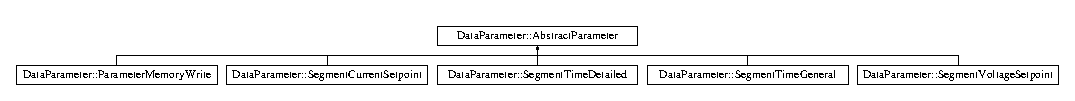
\includegraphics[height=0.910569cm]{da/dfc/class_data_parameter_1_1_abstract_parameter}
\end{center}
\end{figure}
\subsection*{Public Member Functions}
\begin{DoxyCompactItemize}
\item 
\textbf{ Abstract\+Parameter} ()
\begin{DoxyCompactList}\small\item\em \doxyref{Abstract\+Parameter}{p.}{da/dfc/class_data_parameter_1_1_abstract_parameter}. \end{DoxyCompactList}\item 
\textbf{ Abstract\+Parameter} (const int \&code)
\begin{DoxyCompactList}\small\item\em \doxyref{Abstract\+Parameter}{p.}{da/dfc/class_data_parameter_1_1_abstract_parameter}. \end{DoxyCompactList}\item 
virtual \textbf{ Data\+Parameter\+::\+Parameter\+Type} \textbf{ get\+Parameter\+Type} () const =0
\begin{DoxyCompactList}\small\item\em get\+Parameter\+Type \end{DoxyCompactList}\item 
virtual Q\+Byte\+Array \textbf{ get\+Byte\+Array} () const =0
\begin{DoxyCompactList}\small\item\em get\+Byte\+Array \end{DoxyCompactList}\item 
virtual std\+::string \textbf{ get\+Description} () const =0
\begin{DoxyCompactList}\small\item\em get\+Description \end{DoxyCompactList}\item 
void \textbf{ set\+Slave\+Address} (const uint8\+\_\+t \&address)
\begin{DoxyCompactList}\small\item\em set\+Slave\+Address \end{DoxyCompactList}\item 
void \textbf{ set\+Reador\+Write} (const \textbf{ Data\+::\+Read\+Write\+Type} \&type)
\begin{DoxyCompactList}\small\item\em set\+Reador\+Write \end{DoxyCompactList}\item 
Q\+Byte\+Array \textbf{ get\+Full\+Message} ()
\begin{DoxyCompactList}\small\item\em get\+Full\+Message \end{DoxyCompactList}\item 
void \textbf{ operator=} (const \textbf{ Abstract\+Parameter} \&rhs)
\begin{DoxyCompactList}\small\item\em operator = \end{DoxyCompactList}\item 
bool \textbf{ operator==} (const \textbf{ Abstract\+Parameter} \&rhs)
\begin{DoxyCompactList}\small\item\em operator == \end{DoxyCompactList}\item 
bool \textbf{ operator!=} (const \textbf{ Abstract\+Parameter} \&rhs)
\begin{DoxyCompactList}\small\item\em operator != \end{DoxyCompactList}\end{DoxyCompactItemize}
\subsection*{Protected Attributes}
\begin{DoxyCompactItemize}
\item 
int \textbf{ parameter\+Code}
\begin{DoxyCompactList}\small\item\em parameter\+Code \end{DoxyCompactList}\item 
int \textbf{ slave\+Address}
\begin{DoxyCompactList}\small\item\em slave\+Address \end{DoxyCompactList}\item 
\textbf{ Data\+::\+Read\+Write\+Type} \textbf{ read\+Orwrite}
\begin{DoxyCompactList}\small\item\em read\+Orwrite \end{DoxyCompactList}\item 
uint8\+\_\+t \textbf{ high\+Checksum}
\begin{DoxyCompactList}\small\item\em high\+Checksum \end{DoxyCompactList}\item 
uint8\+\_\+t \textbf{ low\+Checksum}
\begin{DoxyCompactList}\small\item\em low\+Checksum \end{DoxyCompactList}\end{DoxyCompactItemize}
\subsection*{Private Member Functions}
\begin{DoxyCompactItemize}
\item 
Q\+Byte\+Array \textbf{ get\+Prefix\+Byte\+Array} ()
\begin{DoxyCompactList}\small\item\em get\+Prefix\+Byte\+Array \end{DoxyCompactList}\item 
unsigned int \textbf{ C\+R\+C16} (const Q\+Byte\+Array \&array)
\begin{DoxyCompactList}\small\item\em C\+R\+C16. \end{DoxyCompactList}\end{DoxyCompactItemize}


\subsection{Detailed Description}
The \doxyref{Abstract\+Parameter}{p.}{da/dfc/class_data_parameter_1_1_abstract_parameter} class. 

Definition at line 20 of file abstract\+\_\+parameter.\+h.



\subsection{Constructor \& Destructor Documentation}
\mbox{\label{class_data_parameter_1_1_abstract_parameter_aabd1ba2f8bf8f174458d5c30b138858b}} 
\index{Data\+Parameter\+::\+Abstract\+Parameter@{Data\+Parameter\+::\+Abstract\+Parameter}!Abstract\+Parameter@{Abstract\+Parameter}}
\index{Abstract\+Parameter@{Abstract\+Parameter}!Data\+Parameter\+::\+Abstract\+Parameter@{Data\+Parameter\+::\+Abstract\+Parameter}}
\subsubsection{Abstract\+Parameter()\hspace{0.1cm}{\footnotesize\ttfamily [1/2]}}
{\footnotesize\ttfamily Data\+Parameter\+::\+Abstract\+Parameter\+::\+Abstract\+Parameter (\begin{DoxyParamCaption}{ }\end{DoxyParamCaption})}



\doxyref{Abstract\+Parameter}{p.}{da/dfc/class_data_parameter_1_1_abstract_parameter}. 



Definition at line 5 of file abstract\+\_\+parameter.\+cpp.

\mbox{\label{class_data_parameter_1_1_abstract_parameter_a15b070524c02d58cb4aeb480790403b3}} 
\index{Data\+Parameter\+::\+Abstract\+Parameter@{Data\+Parameter\+::\+Abstract\+Parameter}!Abstract\+Parameter@{Abstract\+Parameter}}
\index{Abstract\+Parameter@{Abstract\+Parameter}!Data\+Parameter\+::\+Abstract\+Parameter@{Data\+Parameter\+::\+Abstract\+Parameter}}
\subsubsection{Abstract\+Parameter()\hspace{0.1cm}{\footnotesize\ttfamily [2/2]}}
{\footnotesize\ttfamily Data\+Parameter\+::\+Abstract\+Parameter\+::\+Abstract\+Parameter (\begin{DoxyParamCaption}\item[{const int \&}]{code }\end{DoxyParamCaption})}



\doxyref{Abstract\+Parameter}{p.}{da/dfc/class_data_parameter_1_1_abstract_parameter}. 


\begin{DoxyParams}{Parameters}
{\em code} & \\
\hline
\end{DoxyParams}


Definition at line 11 of file abstract\+\_\+parameter.\+cpp.



\subsection{Member Function Documentation}
\mbox{\label{class_data_parameter_1_1_abstract_parameter_a4d7c757c431d45232bf6598b384a68c1}} 
\index{Data\+Parameter\+::\+Abstract\+Parameter@{Data\+Parameter\+::\+Abstract\+Parameter}!C\+R\+C16@{C\+R\+C16}}
\index{C\+R\+C16@{C\+R\+C16}!Data\+Parameter\+::\+Abstract\+Parameter@{Data\+Parameter\+::\+Abstract\+Parameter}}
\subsubsection{C\+R\+C16()}
{\footnotesize\ttfamily unsigned int Data\+Parameter\+::\+Abstract\+Parameter\+::\+C\+R\+C16 (\begin{DoxyParamCaption}\item[{const Q\+Byte\+Array \&}]{array }\end{DoxyParamCaption})\hspace{0.3cm}{\ttfamily [private]}}



C\+R\+C16. 


\begin{DoxyParams}{Parameters}
{\em array} & \\
\hline
\end{DoxyParams}
\begin{DoxyReturn}{Returns}

\end{DoxyReturn}


Definition at line 54 of file abstract\+\_\+parameter.\+cpp.

\mbox{\label{class_data_parameter_1_1_abstract_parameter_aa170d4993cbcf85110dac80813050284}} 
\index{Data\+Parameter\+::\+Abstract\+Parameter@{Data\+Parameter\+::\+Abstract\+Parameter}!get\+Byte\+Array@{get\+Byte\+Array}}
\index{get\+Byte\+Array@{get\+Byte\+Array}!Data\+Parameter\+::\+Abstract\+Parameter@{Data\+Parameter\+::\+Abstract\+Parameter}}
\subsubsection{get\+Byte\+Array()}
{\footnotesize\ttfamily virtual Q\+Byte\+Array Data\+Parameter\+::\+Abstract\+Parameter\+::get\+Byte\+Array (\begin{DoxyParamCaption}{ }\end{DoxyParamCaption}) const\hspace{0.3cm}{\ttfamily [pure virtual]}}



get\+Byte\+Array 

\begin{DoxyReturn}{Returns}

\end{DoxyReturn}


Implemented in \textbf{ Data\+Parameter\+::\+Segment\+Time\+General} \doxyref{}{p.}{df/dd9/class_data_parameter_1_1_segment_time_general_a3a1ac47912c0dafd79e1ababdc856462}, \textbf{ Data\+Parameter\+::\+Segment\+Voltage\+Setpoint} \doxyref{}{p.}{d0/dd0/class_data_parameter_1_1_segment_voltage_setpoint_ad235d797a7a6f02096ad8dd432ee57f7}, \textbf{ Data\+Parameter\+::\+Segment\+Time\+Detailed} \doxyref{}{p.}{de/d8e/class_data_parameter_1_1_segment_time_detailed_a2f55e06ca21950d3624b5d510abbec7d}, \textbf{ Data\+Parameter\+::\+Segment\+Current\+Setpoint} \doxyref{}{p.}{d0/de7/class_data_parameter_1_1_segment_current_setpoint_a960510acca9f82347ee21701e9aabd26}, and \textbf{ Data\+Parameter\+::\+Parameter\+Memory\+Write} \doxyref{}{p.}{d7/d4a/class_data_parameter_1_1_parameter_memory_write_a73a307fad1a09ec2d30e79689c7bf4c5}.

\mbox{\label{class_data_parameter_1_1_abstract_parameter_a48ad1857ea1ad5fb9ca9aceeabf82ba9}} 
\index{Data\+Parameter\+::\+Abstract\+Parameter@{Data\+Parameter\+::\+Abstract\+Parameter}!get\+Description@{get\+Description}}
\index{get\+Description@{get\+Description}!Data\+Parameter\+::\+Abstract\+Parameter@{Data\+Parameter\+::\+Abstract\+Parameter}}
\subsubsection{get\+Description()}
{\footnotesize\ttfamily virtual std\+::string Data\+Parameter\+::\+Abstract\+Parameter\+::get\+Description (\begin{DoxyParamCaption}{ }\end{DoxyParamCaption}) const\hspace{0.3cm}{\ttfamily [pure virtual]}}



get\+Description 

\begin{DoxyReturn}{Returns}

\end{DoxyReturn}


Implemented in \textbf{ Data\+Parameter\+::\+Segment\+Time\+General} \doxyref{}{p.}{df/dd9/class_data_parameter_1_1_segment_time_general_a27d5b594669fdff0d6638c8d3c7d6707}, \textbf{ Data\+Parameter\+::\+Segment\+Time\+Detailed} \doxyref{}{p.}{de/d8e/class_data_parameter_1_1_segment_time_detailed_a20e9b38ddc4452e2f63246aaa1c02f86}, \textbf{ Data\+Parameter\+::\+Segment\+Current\+Setpoint} \doxyref{}{p.}{d0/de7/class_data_parameter_1_1_segment_current_setpoint_a03ce6d68d5c9d3fd6792f2f55d1f875c}, \textbf{ Data\+Parameter\+::\+Segment\+Voltage\+Setpoint} \doxyref{}{p.}{d0/dd0/class_data_parameter_1_1_segment_voltage_setpoint_acabde393bbee6dd5abe4c3d682fc2ee5}, and \textbf{ Data\+Parameter\+::\+Parameter\+Memory\+Write} \doxyref{}{p.}{d7/d4a/class_data_parameter_1_1_parameter_memory_write_a428e813f7c1e2b8d155ffb15a69a405e}.

\mbox{\label{class_data_parameter_1_1_abstract_parameter_a872b9c3f9bca772414de6ee77ea09a28}} 
\index{Data\+Parameter\+::\+Abstract\+Parameter@{Data\+Parameter\+::\+Abstract\+Parameter}!get\+Full\+Message@{get\+Full\+Message}}
\index{get\+Full\+Message@{get\+Full\+Message}!Data\+Parameter\+::\+Abstract\+Parameter@{Data\+Parameter\+::\+Abstract\+Parameter}}
\subsubsection{get\+Full\+Message()}
{\footnotesize\ttfamily Q\+Byte\+Array Data\+Parameter\+::\+Abstract\+Parameter\+::get\+Full\+Message (\begin{DoxyParamCaption}{ }\end{DoxyParamCaption})}



get\+Full\+Message 

\begin{DoxyReturn}{Returns}

\end{DoxyReturn}


Definition at line 40 of file abstract\+\_\+parameter.\+cpp.

\mbox{\label{class_data_parameter_1_1_abstract_parameter_a5566a8d4357cc077dddd856569fe9bbb}} 
\index{Data\+Parameter\+::\+Abstract\+Parameter@{Data\+Parameter\+::\+Abstract\+Parameter}!get\+Parameter\+Type@{get\+Parameter\+Type}}
\index{get\+Parameter\+Type@{get\+Parameter\+Type}!Data\+Parameter\+::\+Abstract\+Parameter@{Data\+Parameter\+::\+Abstract\+Parameter}}
\subsubsection{get\+Parameter\+Type()}
{\footnotesize\ttfamily virtual \textbf{ Data\+Parameter\+::\+Parameter\+Type} Data\+Parameter\+::\+Abstract\+Parameter\+::get\+Parameter\+Type (\begin{DoxyParamCaption}{ }\end{DoxyParamCaption}) const\hspace{0.3cm}{\ttfamily [pure virtual]}}



get\+Parameter\+Type 

\begin{DoxyReturn}{Returns}

\end{DoxyReturn}


Implemented in \textbf{ Data\+Parameter\+::\+Segment\+Time\+General} \doxyref{}{p.}{df/dd9/class_data_parameter_1_1_segment_time_general_aff90789e3919a83f017c6d34c7721447}, \textbf{ Data\+Parameter\+::\+Segment\+Time\+Detailed} \doxyref{}{p.}{de/d8e/class_data_parameter_1_1_segment_time_detailed_ab50e5ee5b8328d6d5b436beb6ae5a262}, \textbf{ Data\+Parameter\+::\+Segment\+Current\+Setpoint} \doxyref{}{p.}{d0/de7/class_data_parameter_1_1_segment_current_setpoint_ae4775df0c99e1b5fd21afbb612d8c02e}, \textbf{ Data\+Parameter\+::\+Segment\+Voltage\+Setpoint} \doxyref{}{p.}{d0/dd0/class_data_parameter_1_1_segment_voltage_setpoint_aa94a5c65dade8f499b3781d8401f2ddd}, and \textbf{ Data\+Parameter\+::\+Parameter\+Memory\+Write} \doxyref{}{p.}{d7/d4a/class_data_parameter_1_1_parameter_memory_write_ae7903da3c10697fac4fb5517bf53e98d}.

\mbox{\label{class_data_parameter_1_1_abstract_parameter_a5e6ec11edb90b7c45fe59ec8376a03ac}} 
\index{Data\+Parameter\+::\+Abstract\+Parameter@{Data\+Parameter\+::\+Abstract\+Parameter}!get\+Prefix\+Byte\+Array@{get\+Prefix\+Byte\+Array}}
\index{get\+Prefix\+Byte\+Array@{get\+Prefix\+Byte\+Array}!Data\+Parameter\+::\+Abstract\+Parameter@{Data\+Parameter\+::\+Abstract\+Parameter}}
\subsubsection{get\+Prefix\+Byte\+Array()}
{\footnotesize\ttfamily Q\+Byte\+Array Data\+Parameter\+::\+Abstract\+Parameter\+::get\+Prefix\+Byte\+Array (\begin{DoxyParamCaption}{ }\end{DoxyParamCaption})\hspace{0.3cm}{\ttfamily [private]}}



get\+Prefix\+Byte\+Array 

\begin{DoxyReturn}{Returns}

\end{DoxyReturn}


Definition at line 27 of file abstract\+\_\+parameter.\+cpp.

\mbox{\label{class_data_parameter_1_1_abstract_parameter_aeecfa3fc5c8452bce00ee8e9f8482769}} 
\index{Data\+Parameter\+::\+Abstract\+Parameter@{Data\+Parameter\+::\+Abstract\+Parameter}!operator"!=@{operator"!=}}
\index{operator"!=@{operator"!=}!Data\+Parameter\+::\+Abstract\+Parameter@{Data\+Parameter\+::\+Abstract\+Parameter}}
\subsubsection{operator"!=()}
{\footnotesize\ttfamily bool Data\+Parameter\+::\+Abstract\+Parameter\+::operator!= (\begin{DoxyParamCaption}\item[{const \textbf{ Abstract\+Parameter} \&}]{rhs }\end{DoxyParamCaption})\hspace{0.3cm}{\ttfamily [inline]}}



operator != 


\begin{DoxyParams}{Parameters}
{\em rhs} & \\
\hline
\end{DoxyParams}
\begin{DoxyReturn}{Returns}

\end{DoxyReturn}


Definition at line 123 of file abstract\+\_\+parameter.\+h.

\mbox{\label{class_data_parameter_1_1_abstract_parameter_a9a39c529f3c5824ca78c37347d18bfe5}} 
\index{Data\+Parameter\+::\+Abstract\+Parameter@{Data\+Parameter\+::\+Abstract\+Parameter}!operator=@{operator=}}
\index{operator=@{operator=}!Data\+Parameter\+::\+Abstract\+Parameter@{Data\+Parameter\+::\+Abstract\+Parameter}}
\subsubsection{operator=()}
{\footnotesize\ttfamily void Data\+Parameter\+::\+Abstract\+Parameter\+::operator= (\begin{DoxyParamCaption}\item[{const \textbf{ Abstract\+Parameter} \&}]{rhs }\end{DoxyParamCaption})\hspace{0.3cm}{\ttfamily [inline]}}



operator = 


\begin{DoxyParams}{Parameters}
{\em rhs} & \\
\hline
\end{DoxyParams}


Definition at line 84 of file abstract\+\_\+parameter.\+h.

\mbox{\label{class_data_parameter_1_1_abstract_parameter_a5aceb144d9b4406c6b0811279681203e}} 
\index{Data\+Parameter\+::\+Abstract\+Parameter@{Data\+Parameter\+::\+Abstract\+Parameter}!operator==@{operator==}}
\index{operator==@{operator==}!Data\+Parameter\+::\+Abstract\+Parameter@{Data\+Parameter\+::\+Abstract\+Parameter}}
\subsubsection{operator==()}
{\footnotesize\ttfamily bool Data\+Parameter\+::\+Abstract\+Parameter\+::operator== (\begin{DoxyParamCaption}\item[{const \textbf{ Abstract\+Parameter} \&}]{rhs }\end{DoxyParamCaption})\hspace{0.3cm}{\ttfamily [inline]}}



operator == 


\begin{DoxyParams}{Parameters}
{\em rhs} & \\
\hline
\end{DoxyParams}
\begin{DoxyReturn}{Returns}

\end{DoxyReturn}


Definition at line 98 of file abstract\+\_\+parameter.\+h.

\mbox{\label{class_data_parameter_1_1_abstract_parameter_a2b6e3c1e1b32da3a92f9ca5218bd8704}} 
\index{Data\+Parameter\+::\+Abstract\+Parameter@{Data\+Parameter\+::\+Abstract\+Parameter}!set\+Reador\+Write@{set\+Reador\+Write}}
\index{set\+Reador\+Write@{set\+Reador\+Write}!Data\+Parameter\+::\+Abstract\+Parameter@{Data\+Parameter\+::\+Abstract\+Parameter}}
\subsubsection{set\+Reador\+Write()}
{\footnotesize\ttfamily void Data\+Parameter\+::\+Abstract\+Parameter\+::set\+Reador\+Write (\begin{DoxyParamCaption}\item[{const \textbf{ Data\+::\+Read\+Write\+Type} \&}]{type }\end{DoxyParamCaption})}



set\+Reador\+Write 


\begin{DoxyParams}{Parameters}
{\em type} & \\
\hline
\end{DoxyParams}


Definition at line 22 of file abstract\+\_\+parameter.\+cpp.

\mbox{\label{class_data_parameter_1_1_abstract_parameter_a3ff19d5948c23dbdb11605250dbd9a71}} 
\index{Data\+Parameter\+::\+Abstract\+Parameter@{Data\+Parameter\+::\+Abstract\+Parameter}!set\+Slave\+Address@{set\+Slave\+Address}}
\index{set\+Slave\+Address@{set\+Slave\+Address}!Data\+Parameter\+::\+Abstract\+Parameter@{Data\+Parameter\+::\+Abstract\+Parameter}}
\subsubsection{set\+Slave\+Address()}
{\footnotesize\ttfamily void Data\+Parameter\+::\+Abstract\+Parameter\+::set\+Slave\+Address (\begin{DoxyParamCaption}\item[{const uint8\+\_\+t \&}]{address }\end{DoxyParamCaption})}



set\+Slave\+Address 


\begin{DoxyParams}{Parameters}
{\em address} & \\
\hline
\end{DoxyParams}


Definition at line 17 of file abstract\+\_\+parameter.\+cpp.



\subsection{Member Data Documentation}
\mbox{\label{class_data_parameter_1_1_abstract_parameter_a0eff8d171e8801fd912b981e779fe54a}} 
\index{Data\+Parameter\+::\+Abstract\+Parameter@{Data\+Parameter\+::\+Abstract\+Parameter}!high\+Checksum@{high\+Checksum}}
\index{high\+Checksum@{high\+Checksum}!Data\+Parameter\+::\+Abstract\+Parameter@{Data\+Parameter\+::\+Abstract\+Parameter}}
\subsubsection{high\+Checksum}
{\footnotesize\ttfamily uint8\+\_\+t Data\+Parameter\+::\+Abstract\+Parameter\+::high\+Checksum\hspace{0.3cm}{\ttfamily [protected]}}



high\+Checksum 



Definition at line 154 of file abstract\+\_\+parameter.\+h.

\mbox{\label{class_data_parameter_1_1_abstract_parameter_a1c8874ec3aa2c359c8b2e4368112701d}} 
\index{Data\+Parameter\+::\+Abstract\+Parameter@{Data\+Parameter\+::\+Abstract\+Parameter}!low\+Checksum@{low\+Checksum}}
\index{low\+Checksum@{low\+Checksum}!Data\+Parameter\+::\+Abstract\+Parameter@{Data\+Parameter\+::\+Abstract\+Parameter}}
\subsubsection{low\+Checksum}
{\footnotesize\ttfamily uint8\+\_\+t Data\+Parameter\+::\+Abstract\+Parameter\+::low\+Checksum\hspace{0.3cm}{\ttfamily [protected]}}



low\+Checksum 



Definition at line 159 of file abstract\+\_\+parameter.\+h.

\mbox{\label{class_data_parameter_1_1_abstract_parameter_aa1e08311a9936590082ac915c7780bb9}} 
\index{Data\+Parameter\+::\+Abstract\+Parameter@{Data\+Parameter\+::\+Abstract\+Parameter}!parameter\+Code@{parameter\+Code}}
\index{parameter\+Code@{parameter\+Code}!Data\+Parameter\+::\+Abstract\+Parameter@{Data\+Parameter\+::\+Abstract\+Parameter}}
\subsubsection{parameter\+Code}
{\footnotesize\ttfamily int Data\+Parameter\+::\+Abstract\+Parameter\+::parameter\+Code\hspace{0.3cm}{\ttfamily [protected]}}



parameter\+Code 



Definition at line 139 of file abstract\+\_\+parameter.\+h.

\mbox{\label{class_data_parameter_1_1_abstract_parameter_a5f73b273bcde383d3fed19690e2e1c53}} 
\index{Data\+Parameter\+::\+Abstract\+Parameter@{Data\+Parameter\+::\+Abstract\+Parameter}!read\+Orwrite@{read\+Orwrite}}
\index{read\+Orwrite@{read\+Orwrite}!Data\+Parameter\+::\+Abstract\+Parameter@{Data\+Parameter\+::\+Abstract\+Parameter}}
\subsubsection{read\+Orwrite}
{\footnotesize\ttfamily \textbf{ Data\+::\+Read\+Write\+Type} Data\+Parameter\+::\+Abstract\+Parameter\+::read\+Orwrite\hspace{0.3cm}{\ttfamily [protected]}}



read\+Orwrite 



Definition at line 149 of file abstract\+\_\+parameter.\+h.

\mbox{\label{class_data_parameter_1_1_abstract_parameter_ae8d47faafbbce3bf4a693af58d1db7b3}} 
\index{Data\+Parameter\+::\+Abstract\+Parameter@{Data\+Parameter\+::\+Abstract\+Parameter}!slave\+Address@{slave\+Address}}
\index{slave\+Address@{slave\+Address}!Data\+Parameter\+::\+Abstract\+Parameter@{Data\+Parameter\+::\+Abstract\+Parameter}}
\subsubsection{slave\+Address}
{\footnotesize\ttfamily int Data\+Parameter\+::\+Abstract\+Parameter\+::slave\+Address\hspace{0.3cm}{\ttfamily [protected]}}



slave\+Address 



Definition at line 144 of file abstract\+\_\+parameter.\+h.



The documentation for this class was generated from the following files\+:\begin{DoxyCompactItemize}
\item 
src/library\+\_\+munk\+\_\+power\+\_\+supply/data\+\_\+registers/\textbf{ abstract\+\_\+parameter.\+h}\item 
src/library\+\_\+munk\+\_\+power\+\_\+supply/data\+\_\+registers/\textbf{ abstract\+\_\+parameter.\+cpp}\end{DoxyCompactItemize}

\section{Common Class Reference}
\label{class_common}\index{Common@{Common}}


{\ttfamily \#include $<$common.\+h$>$}

\subsection*{Public Member Functions}
\begin{DoxyCompactItemize}
\item 
\textbf{ Common} ()
\end{DoxyCompactItemize}


\subsection{Detailed Description}


Definition at line 9 of file common.\+h.



\subsection{Constructor \& Destructor Documentation}
\mbox{\label{class_common_ab0898f6608707a3e07c22d88ecdae661}} 
\index{Common@{Common}!Common@{Common}}
\index{Common@{Common}!Common@{Common}}
\subsubsection{Common()}
{\footnotesize\ttfamily Common\+::\+Common (\begin{DoxyParamCaption}{ }\end{DoxyParamCaption})}



Definition at line 4 of file common.\+cpp.



The documentation for this class was generated from the following files\+:\begin{DoxyCompactItemize}
\item 
src/common/\textbf{ common.\+h}\item 
src/common/\textbf{ common.\+cpp}\end{DoxyCompactItemize}

\section{Exception\+Response Class Reference}
\label{class_exception_response}\index{Exception\+Response@{Exception\+Response}}


{\ttfamily \#include $<$exception\+\_\+response.\+h$>$}

\subsection*{Public Member Functions}
\begin{DoxyCompactItemize}
\item 
\textbf{ Exception\+Response} ()
\end{DoxyCompactItemize}


\subsection{Detailed Description}


Definition at line 5 of file exception\+\_\+response.\+h.



\subsection{Constructor \& Destructor Documentation}
\mbox{\label{class_exception_response_af487015ab89a8e3a4cdc3d5fcf220186}} 
\index{Exception\+Response@{Exception\+Response}!Exception\+Response@{Exception\+Response}}
\index{Exception\+Response@{Exception\+Response}!Exception\+Response@{Exception\+Response}}
\subsubsection{Exception\+Response()}
{\footnotesize\ttfamily Exception\+Response\+::\+Exception\+Response (\begin{DoxyParamCaption}{ }\end{DoxyParamCaption})}



Definition at line 3 of file exception\+\_\+response.\+cpp.



The documentation for this class was generated from the following files\+:\begin{DoxyCompactItemize}
\item 
src/library\+\_\+munk\+\_\+power\+\_\+supply/data\+\_\+response/\textbf{ exception\+\_\+response.\+h}\item 
src/library\+\_\+munk\+\_\+power\+\_\+supply/data\+\_\+response/\textbf{ exception\+\_\+response.\+cpp}\end{DoxyCompactItemize}

\section{Fault\+Register\+One Class Reference}
\label{class_fault_register_one}\index{Fault\+Register\+One@{Fault\+Register\+One}}


{\ttfamily \#include $<$fault\+\_\+register\+\_\+one.\+h$>$}

\subsection*{Public Member Functions}
\begin{DoxyCompactItemize}
\item 
\textbf{ Fault\+Register\+One} ()
\end{DoxyCompactItemize}


\subsection{Detailed Description}


Definition at line 5 of file fault\+\_\+register\+\_\+one.\+h.



\subsection{Constructor \& Destructor Documentation}
\mbox{\label{class_fault_register_one_a2b7823f17c65239256861f3c3120c569}} 
\index{Fault\+Register\+One@{Fault\+Register\+One}!Fault\+Register\+One@{Fault\+Register\+One}}
\index{Fault\+Register\+One@{Fault\+Register\+One}!Fault\+Register\+One@{Fault\+Register\+One}}
\subsubsection{Fault\+Register\+One()}
{\footnotesize\ttfamily Fault\+Register\+One\+::\+Fault\+Register\+One (\begin{DoxyParamCaption}{ }\end{DoxyParamCaption})}



Definition at line 3 of file fault\+\_\+register\+\_\+one.\+cpp.



The documentation for this class was generated from the following files\+:\begin{DoxyCompactItemize}
\item 
src/library\+\_\+munk\+\_\+power\+\_\+supply/data\+\_\+response/\textbf{ fault\+\_\+register\+\_\+one.\+h}\item 
src/library\+\_\+munk\+\_\+power\+\_\+supply/data\+\_\+response/\textbf{ fault\+\_\+register\+\_\+one.\+cpp}\end{DoxyCompactItemize}

\section{Fault\+Register\+Three Class Reference}
\label{class_fault_register_three}\index{Fault\+Register\+Three@{Fault\+Register\+Three}}


{\ttfamily \#include $<$fault\+\_\+register\+\_\+three.\+h$>$}

\subsection*{Public Member Functions}
\begin{DoxyCompactItemize}
\item 
\textbf{ Fault\+Register\+Three} ()
\end{DoxyCompactItemize}


\subsection{Detailed Description}


Definition at line 5 of file fault\+\_\+register\+\_\+three.\+h.



\subsection{Constructor \& Destructor Documentation}
\mbox{\label{class_fault_register_three_a145488e5c4106e3d4a7ad997948d642d}} 
\index{Fault\+Register\+Three@{Fault\+Register\+Three}!Fault\+Register\+Three@{Fault\+Register\+Three}}
\index{Fault\+Register\+Three@{Fault\+Register\+Three}!Fault\+Register\+Three@{Fault\+Register\+Three}}
\subsubsection{Fault\+Register\+Three()}
{\footnotesize\ttfamily Fault\+Register\+Three\+::\+Fault\+Register\+Three (\begin{DoxyParamCaption}{ }\end{DoxyParamCaption})}



Definition at line 3 of file fault\+\_\+register\+\_\+three.\+cpp.



The documentation for this class was generated from the following files\+:\begin{DoxyCompactItemize}
\item 
src/library\+\_\+munk\+\_\+power\+\_\+supply/data\+\_\+response/\textbf{ fault\+\_\+register\+\_\+three.\+h}\item 
src/library\+\_\+munk\+\_\+power\+\_\+supply/data\+\_\+response/\textbf{ fault\+\_\+register\+\_\+three.\+cpp}\end{DoxyCompactItemize}

\section{Fault\+Register\+Two Class Reference}
\label{class_fault_register_two}\index{Fault\+Register\+Two@{Fault\+Register\+Two}}


{\ttfamily \#include $<$fault\+\_\+register\+\_\+two.\+h$>$}

\subsection*{Public Member Functions}
\begin{DoxyCompactItemize}
\item 
\textbf{ Fault\+Register\+Two} ()
\end{DoxyCompactItemize}


\subsection{Detailed Description}


Definition at line 5 of file fault\+\_\+register\+\_\+two.\+h.



\subsection{Constructor \& Destructor Documentation}
\mbox{\label{class_fault_register_two_a0af9cc7c92a39c89034e74bd480e06bb}} 
\index{Fault\+Register\+Two@{Fault\+Register\+Two}!Fault\+Register\+Two@{Fault\+Register\+Two}}
\index{Fault\+Register\+Two@{Fault\+Register\+Two}!Fault\+Register\+Two@{Fault\+Register\+Two}}
\subsubsection{Fault\+Register\+Two()}
{\footnotesize\ttfamily Fault\+Register\+Two\+::\+Fault\+Register\+Two (\begin{DoxyParamCaption}{ }\end{DoxyParamCaption})}



Definition at line 3 of file fault\+\_\+register\+\_\+two.\+cpp.



The documentation for this class was generated from the following files\+:\begin{DoxyCompactItemize}
\item 
src/library\+\_\+munk\+\_\+power\+\_\+supply/data\+\_\+response/\textbf{ fault\+\_\+register\+\_\+two.\+h}\item 
src/library\+\_\+munk\+\_\+power\+\_\+supply/data\+\_\+response/\textbf{ fault\+\_\+register\+\_\+two.\+cpp}\end{DoxyCompactItemize}

\section{Ui\+:\+:Main\+Window Class Reference}
\label{class_ui_1_1_main_window}\index{Ui\+::\+Main\+Window@{Ui\+::\+Main\+Window}}


{\ttfamily \#include $<$ui\+\_\+mainwindow.\+h$>$}

Inheritance diagram for Ui\+:\+:Main\+Window\+:\begin{figure}[H]
\begin{center}
\leavevmode
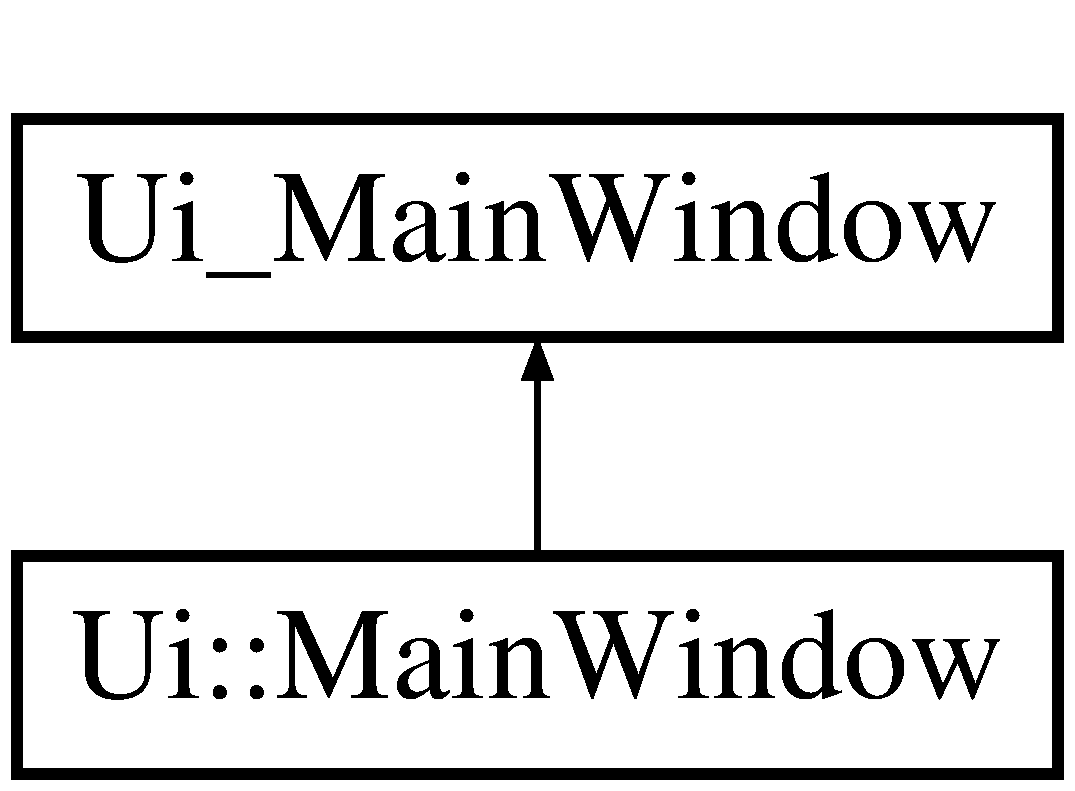
\includegraphics[height=2.000000cm]{d4/d4a/class_ui_1_1_main_window}
\end{center}
\end{figure}
\subsection*{Additional Inherited Members}


\subsection{Detailed Description}


Definition at line 64 of file ui\+\_\+mainwindow.\+h.



The documentation for this class was generated from the following file\+:\begin{DoxyCompactItemize}
\item 
src/\+E\+C\+M\+\_\+\+Main\+Window/\textbf{ ui\+\_\+mainwindow.\+h}\end{DoxyCompactItemize}

\section{Main\+Window Class Reference}
\label{class_main_window}\index{Main\+Window@{Main\+Window}}


{\ttfamily \#include $<$mainwindow.\+h$>$}

Inheritance diagram for Main\+Window\+:\begin{figure}[H]
\begin{center}
\leavevmode
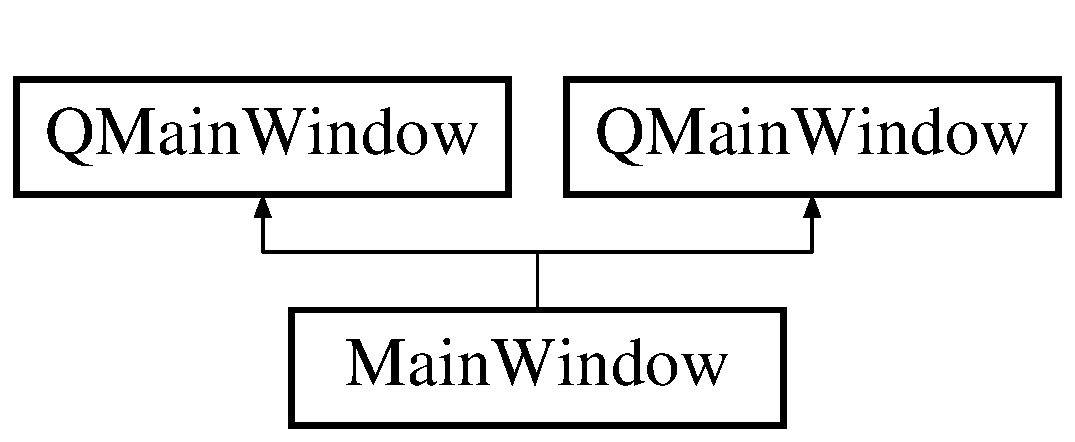
\includegraphics[height=2.000000cm]{d9/dc6/class_main_window}
\end{center}
\end{figure}
\subsection*{Public Slots}
\begin{DoxyCompactItemize}
\item 
void \textbf{ generate\+Message} ()
\end{DoxyCompactItemize}
\subsection*{Public Member Functions}
\begin{DoxyCompactItemize}
\item 
\textbf{ Main\+Window} (Q\+Widget $\ast$parent=0)
\item 
\textbf{ $\sim$\+Main\+Window} ()
\item 
\textbf{ Main\+Window} (Q\+Widget $\ast$parent=0)
\item 
\textbf{ $\sim$\+Main\+Window} ()
\item 
void \textbf{ setup\+Ui\+Elements} ()
\end{DoxyCompactItemize}
\subsection*{Private Slots}
\begin{DoxyCompactItemize}
\item 
void \textbf{ on\+\_\+push\+Button\+\_\+generatemsg\+\_\+clicked} ()
\end{DoxyCompactItemize}
\subsection*{Private Attributes}
\begin{DoxyCompactItemize}
\item 
\textbf{ Ui\+::\+Main\+Window} $\ast$ \textbf{ ui}
\end{DoxyCompactItemize}


\subsection{Detailed Description}


Definition at line 19 of file mainwindow.\+h.



\subsection{Constructor \& Destructor Documentation}
\mbox{\label{class_main_window_a8b244be8b7b7db1b08de2a2acb9409db}} 
\index{Main\+Window@{Main\+Window}!Main\+Window@{Main\+Window}}
\index{Main\+Window@{Main\+Window}!Main\+Window@{Main\+Window}}
\subsubsection{Main\+Window()\hspace{0.1cm}{\footnotesize\ttfamily [1/2]}}
{\footnotesize\ttfamily Main\+Window\+::\+Main\+Window (\begin{DoxyParamCaption}\item[{Q\+Widget $\ast$}]{parent = {\ttfamily 0} }\end{DoxyParamCaption})\hspace{0.3cm}{\ttfamily [explicit]}}



Definition at line 4 of file mainwindow.\+cpp.

\mbox{\label{class_main_window_ae98d00a93bc118200eeef9f9bba1dba7}} 
\index{Main\+Window@{Main\+Window}!````~Main\+Window@{$\sim$\+Main\+Window}}
\index{````~Main\+Window@{$\sim$\+Main\+Window}!Main\+Window@{Main\+Window}}
\subsubsection{$\sim$\+Main\+Window()\hspace{0.1cm}{\footnotesize\ttfamily [1/2]}}
{\footnotesize\ttfamily Main\+Window\+::$\sim$\+Main\+Window (\begin{DoxyParamCaption}{ }\end{DoxyParamCaption})}



Definition at line 12 of file mainwindow.\+cpp.

\mbox{\label{class_main_window_a8b244be8b7b7db1b08de2a2acb9409db}} 
\index{Main\+Window@{Main\+Window}!Main\+Window@{Main\+Window}}
\index{Main\+Window@{Main\+Window}!Main\+Window@{Main\+Window}}
\subsubsection{Main\+Window()\hspace{0.1cm}{\footnotesize\ttfamily [2/2]}}
{\footnotesize\ttfamily Main\+Window\+::\+Main\+Window (\begin{DoxyParamCaption}\item[{Q\+Widget $\ast$}]{parent = {\ttfamily 0} }\end{DoxyParamCaption})\hspace{0.3cm}{\ttfamily [explicit]}}

\mbox{\label{class_main_window_ae98d00a93bc118200eeef9f9bba1dba7}} 
\index{Main\+Window@{Main\+Window}!````~Main\+Window@{$\sim$\+Main\+Window}}
\index{````~Main\+Window@{$\sim$\+Main\+Window}!Main\+Window@{Main\+Window}}
\subsubsection{$\sim$\+Main\+Window()\hspace{0.1cm}{\footnotesize\ttfamily [2/2]}}
{\footnotesize\ttfamily Main\+Window\+::$\sim$\+Main\+Window (\begin{DoxyParamCaption}{ }\end{DoxyParamCaption})}



\subsection{Member Function Documentation}
\mbox{\label{class_main_window_a0cc6d93e4c5ce3e9c4af7f9ba485c34c}} 
\index{Main\+Window@{Main\+Window}!generate\+Message@{generate\+Message}}
\index{generate\+Message@{generate\+Message}!Main\+Window@{Main\+Window}}
\subsubsection{generate\+Message}
{\footnotesize\ttfamily void Main\+Window\+::generate\+Message (\begin{DoxyParamCaption}{ }\end{DoxyParamCaption})\hspace{0.3cm}{\ttfamily [slot]}}



Definition at line 54 of file mainwindow.\+cpp.

\mbox{\label{class_main_window_a83864235c4e3def3355d438ffa6f93bd}} 
\index{Main\+Window@{Main\+Window}!on\+\_\+push\+Button\+\_\+generatemsg\+\_\+clicked@{on\+\_\+push\+Button\+\_\+generatemsg\+\_\+clicked}}
\index{on\+\_\+push\+Button\+\_\+generatemsg\+\_\+clicked@{on\+\_\+push\+Button\+\_\+generatemsg\+\_\+clicked}!Main\+Window@{Main\+Window}}
\subsubsection{on\+\_\+push\+Button\+\_\+generatemsg\+\_\+clicked}
{\footnotesize\ttfamily void Main\+Window\+::on\+\_\+push\+Button\+\_\+generatemsg\+\_\+clicked (\begin{DoxyParamCaption}{ }\end{DoxyParamCaption})\hspace{0.3cm}{\ttfamily [private]}, {\ttfamily [slot]}}



Definition at line 78 of file mainwindow.\+cpp.

\mbox{\label{class_main_window_ac30b6e05110f500244ecd15456a652b0}} 
\index{Main\+Window@{Main\+Window}!setup\+Ui\+Elements@{setup\+Ui\+Elements}}
\index{setup\+Ui\+Elements@{setup\+Ui\+Elements}!Main\+Window@{Main\+Window}}
\subsubsection{setup\+Ui\+Elements()}
{\footnotesize\ttfamily void Main\+Window\+::setup\+Ui\+Elements (\begin{DoxyParamCaption}{ }\end{DoxyParamCaption})}



Definition at line 23 of file mainwindow.\+cpp.



\subsection{Member Data Documentation}
\mbox{\label{class_main_window_a43606649aeaf9e561328935fca0cd1bf}} 
\index{Main\+Window@{Main\+Window}!ui@{ui}}
\index{ui@{ui}!Main\+Window@{Main\+Window}}
\subsubsection{ui}
{\footnotesize\ttfamily \textbf{ Ui\+::\+Main\+Window} $\ast$ Main\+Window\+::ui\hspace{0.3cm}{\ttfamily [private]}}



Definition at line 28 of file mainwindow.\+h.



The documentation for this class was generated from the following files\+:\begin{DoxyCompactItemize}
\item 
src/\+E\+C\+M\+\_\+\+Main\+Window/\textbf{ mainwindow.\+h}\item 
src/\+E\+C\+M\+\_\+\+Main\+Window/\textbf{ mainwindow.\+cpp}\end{DoxyCompactItemize}

\section{Munk\+Power\+Supply Class Reference}
\label{class_munk_power_supply}\index{Munk\+Power\+Supply@{Munk\+Power\+Supply}}


{\ttfamily \#include $<$munk\+\_\+power\+\_\+supply.\+h$>$}

\subsection*{Public Member Functions}
\begin{DoxyCompactItemize}
\item 
\textbf{ Munk\+Power\+Supply} ()
\item 
void \textbf{ generate\+Messages} (const \textbf{ Data\+Parameter\+::\+Segment\+Time\+Detailed} \&detailed\+Segment\+Data)
\end{DoxyCompactItemize}
\subsection*{Private Member Functions}
\begin{DoxyCompactItemize}
\item 
void \textbf{ generate\+Setpoint\+Messages} (const std\+::map$<$ \textbf{ Data\+::\+Register\+Data\+Object}, \textbf{ Data\+::\+Segment\+Level} $>$ \&map, const \textbf{ Data\+::\+Segment\+Mode} \&mode, std\+::vector$<$ \textbf{ Data\+Parameter\+::\+Segment\+Voltage\+Setpoint} $>$ \&V\+Msgs, std\+::vector$<$ \textbf{ Data\+Parameter\+::\+Segment\+Current\+Setpoint} $>$ \&I\+Msgs)
\end{DoxyCompactItemize}


\subsection{Detailed Description}


Definition at line 15 of file munk\+\_\+power\+\_\+supply.\+h.



\subsection{Constructor \& Destructor Documentation}
\mbox{\label{class_munk_power_supply_a4dbb8e589a1a7d7ecdd9c1e20be5c0b8}} 
\index{Munk\+Power\+Supply@{Munk\+Power\+Supply}!Munk\+Power\+Supply@{Munk\+Power\+Supply}}
\index{Munk\+Power\+Supply@{Munk\+Power\+Supply}!Munk\+Power\+Supply@{Munk\+Power\+Supply}}
\subsubsection{Munk\+Power\+Supply()}
{\footnotesize\ttfamily Munk\+Power\+Supply\+::\+Munk\+Power\+Supply (\begin{DoxyParamCaption}{ }\end{DoxyParamCaption})}



Definition at line 3 of file munk\+\_\+power\+\_\+supply.\+cpp.



\subsection{Member Function Documentation}
\mbox{\label{class_munk_power_supply_a93fa50a726abc272287a88f4bec1cc64}} 
\index{Munk\+Power\+Supply@{Munk\+Power\+Supply}!generate\+Messages@{generate\+Messages}}
\index{generate\+Messages@{generate\+Messages}!Munk\+Power\+Supply@{Munk\+Power\+Supply}}
\subsubsection{generate\+Messages()}
{\footnotesize\ttfamily void Munk\+Power\+Supply\+::generate\+Messages (\begin{DoxyParamCaption}\item[{const \textbf{ Data\+Parameter\+::\+Segment\+Time\+Detailed} \&}]{detailed\+Segment\+Data }\end{DoxyParamCaption})}



Definition at line 47 of file munk\+\_\+power\+\_\+supply.\+cpp.

\mbox{\label{class_munk_power_supply_ae24804f05e23d9c3549fe1e2fe149429}} 
\index{Munk\+Power\+Supply@{Munk\+Power\+Supply}!generate\+Setpoint\+Messages@{generate\+Setpoint\+Messages}}
\index{generate\+Setpoint\+Messages@{generate\+Setpoint\+Messages}!Munk\+Power\+Supply@{Munk\+Power\+Supply}}
\subsubsection{generate\+Setpoint\+Messages()}
{\footnotesize\ttfamily void Munk\+Power\+Supply\+::generate\+Setpoint\+Messages (\begin{DoxyParamCaption}\item[{const std\+::map$<$ \textbf{ Data\+::\+Register\+Data\+Object}, \textbf{ Data\+::\+Segment\+Level} $>$ \&}]{map,  }\item[{const \textbf{ Data\+::\+Segment\+Mode} \&}]{mode,  }\item[{std\+::vector$<$ \textbf{ Data\+Parameter\+::\+Segment\+Voltage\+Setpoint} $>$ \&}]{V\+Msgs,  }\item[{std\+::vector$<$ \textbf{ Data\+Parameter\+::\+Segment\+Current\+Setpoint} $>$ \&}]{I\+Msgs }\end{DoxyParamCaption})\hspace{0.3cm}{\ttfamily [private]}}



Definition at line 31 of file munk\+\_\+power\+\_\+supply.\+cpp.



The documentation for this class was generated from the following files\+:\begin{DoxyCompactItemize}
\item 
src/library\+\_\+munk\+\_\+power\+\_\+supply/\textbf{ munk\+\_\+power\+\_\+supply.\+h}\item 
src/library\+\_\+munk\+\_\+power\+\_\+supply/\textbf{ munk\+\_\+power\+\_\+supply.\+cpp}\end{DoxyCompactItemize}

\section{Data\+Parameter\+:\+:Parameter\+Memory\+Write Class Reference}
\label{class_data_parameter_1_1_parameter_memory_write}\index{Data\+Parameter\+::\+Parameter\+Memory\+Write@{Data\+Parameter\+::\+Parameter\+Memory\+Write}}


The \doxyref{Parameter\+Memory\+Write}{p.}{d7/d4a/class_data_parameter_1_1_parameter_memory_write} class.  




{\ttfamily \#include $<$parameter\+\_\+memory\+\_\+write.\+h$>$}

Inheritance diagram for Data\+Parameter\+:\+:Parameter\+Memory\+Write\+:\begin{figure}[H]
\begin{center}
\leavevmode
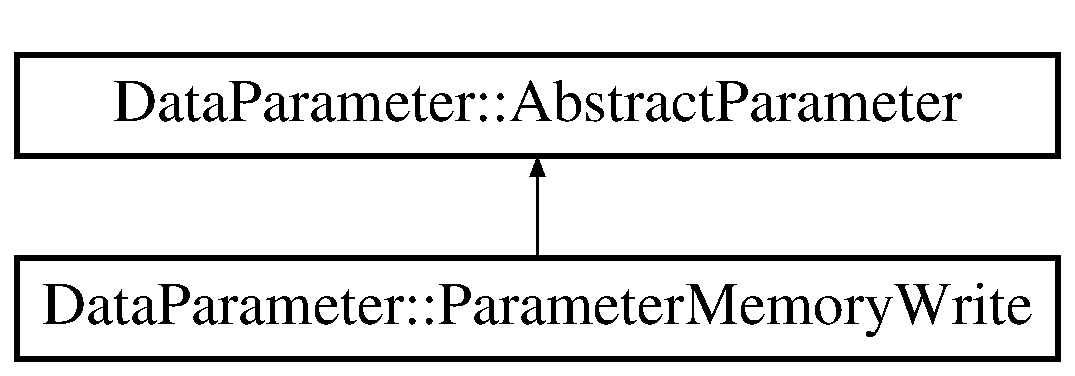
\includegraphics[height=2.000000cm]{d7/d4a/class_data_parameter_1_1_parameter_memory_write}
\end{center}
\end{figure}
\subsection*{Public Member Functions}
\begin{DoxyCompactItemize}
\item 
\textbf{ Parameter\+Memory\+Write} ()
\begin{DoxyCompactList}\small\item\em \doxyref{Parameter\+Memory\+Write}{p.}{d7/d4a/class_data_parameter_1_1_parameter_memory_write}. \end{DoxyCompactList}\item 
virtual \textbf{ Data\+Parameter\+::\+Parameter\+Type} \textbf{ get\+Parameter\+Type} () const
\begin{DoxyCompactList}\small\item\em get\+Parameter\+Type \end{DoxyCompactList}\item 
virtual Q\+Byte\+Array \textbf{ get\+Byte\+Array} () const
\begin{DoxyCompactList}\small\item\em get\+Byte\+Array \end{DoxyCompactList}\item 
virtual std\+::string \textbf{ get\+Description} () const
\begin{DoxyCompactList}\small\item\em get\+Description \end{DoxyCompactList}\end{DoxyCompactItemize}
\subsection*{Additional Inherited Members}


\subsection{Detailed Description}
The \doxyref{Parameter\+Memory\+Write}{p.}{d7/d4a/class_data_parameter_1_1_parameter_memory_write} class. 

Definition at line 15 of file parameter\+\_\+memory\+\_\+write.\+h.



\subsection{Constructor \& Destructor Documentation}
\mbox{\label{class_data_parameter_1_1_parameter_memory_write_a0950f8743a8e5cb2caaa6749133f36e5}} 
\index{Data\+Parameter\+::\+Parameter\+Memory\+Write@{Data\+Parameter\+::\+Parameter\+Memory\+Write}!Parameter\+Memory\+Write@{Parameter\+Memory\+Write}}
\index{Parameter\+Memory\+Write@{Parameter\+Memory\+Write}!Data\+Parameter\+::\+Parameter\+Memory\+Write@{Data\+Parameter\+::\+Parameter\+Memory\+Write}}
\subsubsection{Parameter\+Memory\+Write()}
{\footnotesize\ttfamily Data\+Parameter\+::\+Parameter\+Memory\+Write\+::\+Parameter\+Memory\+Write (\begin{DoxyParamCaption}{ }\end{DoxyParamCaption})}



\doxyref{Parameter\+Memory\+Write}{p.}{d7/d4a/class_data_parameter_1_1_parameter_memory_write}. 



Definition at line 6 of file parameter\+\_\+memory\+\_\+write.\+cpp.



\subsection{Member Function Documentation}
\mbox{\label{class_data_parameter_1_1_parameter_memory_write_a73a307fad1a09ec2d30e79689c7bf4c5}} 
\index{Data\+Parameter\+::\+Parameter\+Memory\+Write@{Data\+Parameter\+::\+Parameter\+Memory\+Write}!get\+Byte\+Array@{get\+Byte\+Array}}
\index{get\+Byte\+Array@{get\+Byte\+Array}!Data\+Parameter\+::\+Parameter\+Memory\+Write@{Data\+Parameter\+::\+Parameter\+Memory\+Write}}
\subsubsection{get\+Byte\+Array()}
{\footnotesize\ttfamily Q\+Byte\+Array Data\+Parameter\+::\+Parameter\+Memory\+Write\+::get\+Byte\+Array (\begin{DoxyParamCaption}{ }\end{DoxyParamCaption}) const\hspace{0.3cm}{\ttfamily [virtual]}}



get\+Byte\+Array 

\begin{DoxyReturn}{Returns}

\end{DoxyReturn}


Implements \textbf{ Data\+Parameter\+::\+Abstract\+Parameter} \doxyref{}{p.}{da/dfc/class_data_parameter_1_1_abstract_parameter_aa170d4993cbcf85110dac80813050284}.



Definition at line 22 of file parameter\+\_\+memory\+\_\+write.\+cpp.

\mbox{\label{class_data_parameter_1_1_parameter_memory_write_a428e813f7c1e2b8d155ffb15a69a405e}} 
\index{Data\+Parameter\+::\+Parameter\+Memory\+Write@{Data\+Parameter\+::\+Parameter\+Memory\+Write}!get\+Description@{get\+Description}}
\index{get\+Description@{get\+Description}!Data\+Parameter\+::\+Parameter\+Memory\+Write@{Data\+Parameter\+::\+Parameter\+Memory\+Write}}
\subsubsection{get\+Description()}
{\footnotesize\ttfamily std\+::string Data\+Parameter\+::\+Parameter\+Memory\+Write\+::get\+Description (\begin{DoxyParamCaption}{ }\end{DoxyParamCaption}) const\hspace{0.3cm}{\ttfamily [virtual]}}



get\+Description 

\begin{DoxyReturn}{Returns}

\end{DoxyReturn}


Implements \textbf{ Data\+Parameter\+::\+Abstract\+Parameter} \doxyref{}{p.}{da/dfc/class_data_parameter_1_1_abstract_parameter_a48ad1857ea1ad5fb9ca9aceeabf82ba9}.



Definition at line 16 of file parameter\+\_\+memory\+\_\+write.\+cpp.

\mbox{\label{class_data_parameter_1_1_parameter_memory_write_ae7903da3c10697fac4fb5517bf53e98d}} 
\index{Data\+Parameter\+::\+Parameter\+Memory\+Write@{Data\+Parameter\+::\+Parameter\+Memory\+Write}!get\+Parameter\+Type@{get\+Parameter\+Type}}
\index{get\+Parameter\+Type@{get\+Parameter\+Type}!Data\+Parameter\+::\+Parameter\+Memory\+Write@{Data\+Parameter\+::\+Parameter\+Memory\+Write}}
\subsubsection{get\+Parameter\+Type()}
{\footnotesize\ttfamily \textbf{ Parameter\+Type} Data\+Parameter\+::\+Parameter\+Memory\+Write\+::get\+Parameter\+Type (\begin{DoxyParamCaption}{ }\end{DoxyParamCaption}) const\hspace{0.3cm}{\ttfamily [virtual]}}



get\+Parameter\+Type 

\begin{DoxyReturn}{Returns}

\end{DoxyReturn}


Implements \textbf{ Data\+Parameter\+::\+Abstract\+Parameter} \doxyref{}{p.}{da/dfc/class_data_parameter_1_1_abstract_parameter_a5566a8d4357cc077dddd856569fe9bbb}.



Definition at line 11 of file parameter\+\_\+memory\+\_\+write.\+cpp.



The documentation for this class was generated from the following files\+:\begin{DoxyCompactItemize}
\item 
src/library\+\_\+munk\+\_\+power\+\_\+supply/data\+\_\+registers/\textbf{ parameter\+\_\+memory\+\_\+write.\+h}\item 
src/library\+\_\+munk\+\_\+power\+\_\+supply/data\+\_\+registers/\textbf{ parameter\+\_\+memory\+\_\+write.\+cpp}\end{DoxyCompactItemize}

\section{Data\+:\+:Register\+Data\+Object Class Reference}
\label{class_data_1_1_register_data_object}\index{Data\+::\+Register\+Data\+Object@{Data\+::\+Register\+Data\+Object}}


The \doxyref{Register\+Data\+Object}{p.}{df/d53/class_data_1_1_register_data_object} class.  




{\ttfamily \#include $<$register\+\_\+data\+\_\+object.\+h$>$}

\subsection*{Public Member Functions}
\begin{DoxyCompactItemize}
\item 
\textbf{ Register\+Data\+Object} ()
\begin{DoxyCompactList}\small\item\em \doxyref{Register\+Data\+Object}{p.}{df/d53/class_data_1_1_register_data_object}. \end{DoxyCompactList}\item 
\textbf{ Register\+Data\+Object} (const int \&\textbf{ voltage}, const int \&\textbf{ current})
\begin{DoxyCompactList}\small\item\em \doxyref{Register\+Data\+Object}{p.}{df/d53/class_data_1_1_register_data_object}. \end{DoxyCompactList}\item 
\textbf{ Register\+Data\+Object} (const \textbf{ Register\+Data\+Object} \&obj)
\begin{DoxyCompactList}\small\item\em \doxyref{Register\+Data\+Object}{p.}{df/d53/class_data_1_1_register_data_object}. \end{DoxyCompactList}\item 
void \textbf{ operator=} (const \textbf{ Register\+Data\+Object} \&rhs)
\begin{DoxyCompactList}\small\item\em operator = \end{DoxyCompactList}\item 
bool \textbf{ operator$<$} (const \textbf{ Register\+Data\+Object} \&rhs) const
\begin{DoxyCompactList}\small\item\em operator $<$ \end{DoxyCompactList}\item 
bool \textbf{ operator==} (const \textbf{ Register\+Data\+Object} \&rhs) const
\begin{DoxyCompactList}\small\item\em operator == \end{DoxyCompactList}\item 
bool \textbf{ operator!=} (const \textbf{ Register\+Data\+Object} \&rhs) const
\begin{DoxyCompactList}\small\item\em operator != \end{DoxyCompactList}\end{DoxyCompactItemize}
\subsection*{Public Attributes}
\begin{DoxyCompactItemize}
\item 
int \textbf{ voltage}
\begin{DoxyCompactList}\small\item\em voltage \end{DoxyCompactList}\item 
int \textbf{ current}
\begin{DoxyCompactList}\small\item\em current \end{DoxyCompactList}\end{DoxyCompactItemize}


\subsection{Detailed Description}
The \doxyref{Register\+Data\+Object}{p.}{df/d53/class_data_1_1_register_data_object} class. 

Definition at line 15 of file register\+\_\+data\+\_\+object.\+h.



\subsection{Constructor \& Destructor Documentation}
\mbox{\label{class_data_1_1_register_data_object_ab7774d694983f85ee9e1626a35c9b391}} 
\index{Data\+::\+Register\+Data\+Object@{Data\+::\+Register\+Data\+Object}!Register\+Data\+Object@{Register\+Data\+Object}}
\index{Register\+Data\+Object@{Register\+Data\+Object}!Data\+::\+Register\+Data\+Object@{Data\+::\+Register\+Data\+Object}}
\subsubsection{Register\+Data\+Object()\hspace{0.1cm}{\footnotesize\ttfamily [1/3]}}
{\footnotesize\ttfamily Data\+::\+Register\+Data\+Object\+::\+Register\+Data\+Object (\begin{DoxyParamCaption}{ }\end{DoxyParamCaption})}



\doxyref{Register\+Data\+Object}{p.}{df/d53/class_data_1_1_register_data_object}. 



Definition at line 5 of file register\+\_\+data\+\_\+object.\+cpp.

\mbox{\label{class_data_1_1_register_data_object_a37f0946ad82917850cf33db16ce4b9b6}} 
\index{Data\+::\+Register\+Data\+Object@{Data\+::\+Register\+Data\+Object}!Register\+Data\+Object@{Register\+Data\+Object}}
\index{Register\+Data\+Object@{Register\+Data\+Object}!Data\+::\+Register\+Data\+Object@{Data\+::\+Register\+Data\+Object}}
\subsubsection{Register\+Data\+Object()\hspace{0.1cm}{\footnotesize\ttfamily [2/3]}}
{\footnotesize\ttfamily Data\+::\+Register\+Data\+Object\+::\+Register\+Data\+Object (\begin{DoxyParamCaption}\item[{const int \&}]{voltage,  }\item[{const int \&}]{current }\end{DoxyParamCaption})}



\doxyref{Register\+Data\+Object}{p.}{df/d53/class_data_1_1_register_data_object}. 


\begin{DoxyParams}{Parameters}
{\em voltage} & \\
\hline
{\em current} & \\
\hline
\end{DoxyParams}


Definition at line 11 of file register\+\_\+data\+\_\+object.\+cpp.

\mbox{\label{class_data_1_1_register_data_object_a4e3aaa00dedd1eba9d4d4921e7e154d2}} 
\index{Data\+::\+Register\+Data\+Object@{Data\+::\+Register\+Data\+Object}!Register\+Data\+Object@{Register\+Data\+Object}}
\index{Register\+Data\+Object@{Register\+Data\+Object}!Data\+::\+Register\+Data\+Object@{Data\+::\+Register\+Data\+Object}}
\subsubsection{Register\+Data\+Object()\hspace{0.1cm}{\footnotesize\ttfamily [3/3]}}
{\footnotesize\ttfamily Data\+::\+Register\+Data\+Object\+::\+Register\+Data\+Object (\begin{DoxyParamCaption}\item[{const \textbf{ Register\+Data\+Object} \&}]{obj }\end{DoxyParamCaption})}



\doxyref{Register\+Data\+Object}{p.}{df/d53/class_data_1_1_register_data_object}. 


\begin{DoxyParams}{Parameters}
{\em obj} & \\
\hline
\end{DoxyParams}


Definition at line 17 of file register\+\_\+data\+\_\+object.\+cpp.



\subsection{Member Function Documentation}
\mbox{\label{class_data_1_1_register_data_object_a6839088034594b4e921e82d6ecbccef9}} 
\index{Data\+::\+Register\+Data\+Object@{Data\+::\+Register\+Data\+Object}!operator"!=@{operator"!=}}
\index{operator"!=@{operator"!=}!Data\+::\+Register\+Data\+Object@{Data\+::\+Register\+Data\+Object}}
\subsubsection{operator"!=()}
{\footnotesize\ttfamily bool Data\+::\+Register\+Data\+Object\+::operator!= (\begin{DoxyParamCaption}\item[{const \textbf{ Register\+Data\+Object} \&}]{rhs }\end{DoxyParamCaption}) const}



operator != 


\begin{DoxyParams}{Parameters}
{\em rhs} & \\
\hline
\end{DoxyParams}
\begin{DoxyReturn}{Returns}

\end{DoxyReturn}


Definition at line 58 of file register\+\_\+data\+\_\+object.\+cpp.

\mbox{\label{class_data_1_1_register_data_object_a13c8205dd0c58e317e67a9872350fed2}} 
\index{Data\+::\+Register\+Data\+Object@{Data\+::\+Register\+Data\+Object}!operator$<$@{operator$<$}}
\index{operator$<$@{operator$<$}!Data\+::\+Register\+Data\+Object@{Data\+::\+Register\+Data\+Object}}
\subsubsection{operator$<$()}
{\footnotesize\ttfamily bool Data\+::\+Register\+Data\+Object\+::operator$<$ (\begin{DoxyParamCaption}\item[{const \textbf{ Register\+Data\+Object} \&}]{rhs }\end{DoxyParamCaption}) const}



operator $<$ 


\begin{DoxyParams}{Parameters}
{\em rhs} & \\
\hline
\end{DoxyParams}
\begin{DoxyReturn}{Returns}

\end{DoxyReturn}


Definition at line 29 of file register\+\_\+data\+\_\+object.\+cpp.

\mbox{\label{class_data_1_1_register_data_object_a8479b834a499d573df2247091a4b12cc}} 
\index{Data\+::\+Register\+Data\+Object@{Data\+::\+Register\+Data\+Object}!operator=@{operator=}}
\index{operator=@{operator=}!Data\+::\+Register\+Data\+Object@{Data\+::\+Register\+Data\+Object}}
\subsubsection{operator=()}
{\footnotesize\ttfamily void Data\+::\+Register\+Data\+Object\+::operator= (\begin{DoxyParamCaption}\item[{const \textbf{ Register\+Data\+Object} \&}]{rhs }\end{DoxyParamCaption})}



operator = 


\begin{DoxyParams}{Parameters}
{\em rhs} & \\
\hline
\end{DoxyParams}


Definition at line 23 of file register\+\_\+data\+\_\+object.\+cpp.

\mbox{\label{class_data_1_1_register_data_object_a49126058b448bd00f5d7d9ec59b28167}} 
\index{Data\+::\+Register\+Data\+Object@{Data\+::\+Register\+Data\+Object}!operator==@{operator==}}
\index{operator==@{operator==}!Data\+::\+Register\+Data\+Object@{Data\+::\+Register\+Data\+Object}}
\subsubsection{operator==()}
{\footnotesize\ttfamily bool Data\+::\+Register\+Data\+Object\+::operator== (\begin{DoxyParamCaption}\item[{const \textbf{ Register\+Data\+Object} \&}]{rhs }\end{DoxyParamCaption}) const}



operator == 


\begin{DoxyParams}{Parameters}
{\em rhs} & \\
\hline
\end{DoxyParams}
\begin{DoxyReturn}{Returns}

\end{DoxyReturn}


Definition at line 49 of file register\+\_\+data\+\_\+object.\+cpp.



\subsection{Member Data Documentation}
\mbox{\label{class_data_1_1_register_data_object_a6dddad550b98fdf7cd1fcfcfff20ffce}} 
\index{Data\+::\+Register\+Data\+Object@{Data\+::\+Register\+Data\+Object}!current@{current}}
\index{current@{current}!Data\+::\+Register\+Data\+Object@{Data\+::\+Register\+Data\+Object}}
\subsubsection{current}
{\footnotesize\ttfamily int Data\+::\+Register\+Data\+Object\+::current}



current 



Definition at line 73 of file register\+\_\+data\+\_\+object.\+h.

\mbox{\label{class_data_1_1_register_data_object_a67abdf7e33ab899281ac4bdbcc33c263}} 
\index{Data\+::\+Register\+Data\+Object@{Data\+::\+Register\+Data\+Object}!voltage@{voltage}}
\index{voltage@{voltage}!Data\+::\+Register\+Data\+Object@{Data\+::\+Register\+Data\+Object}}
\subsubsection{voltage}
{\footnotesize\ttfamily int Data\+::\+Register\+Data\+Object\+::voltage}



voltage 



Definition at line 68 of file register\+\_\+data\+\_\+object.\+h.



The documentation for this class was generated from the following files\+:\begin{DoxyCompactItemize}
\item 
src/library\+\_\+munk\+\_\+power\+\_\+supply/data/\textbf{ register\+\_\+data\+\_\+object.\+h}\item 
src/library\+\_\+munk\+\_\+power\+\_\+supply/data/\textbf{ register\+\_\+data\+\_\+object.\+cpp}\end{DoxyCompactItemize}

\section{Data\+Parameter\+:\+:Segment\+Current\+Setpoint Class Reference}
\label{class_data_parameter_1_1_segment_current_setpoint}\index{Data\+Parameter\+::\+Segment\+Current\+Setpoint@{Data\+Parameter\+::\+Segment\+Current\+Setpoint}}


The \doxyref{Segment\+Current\+Setpoint}{p.}{d0/de7/class_data_parameter_1_1_segment_current_setpoint} class.  




{\ttfamily \#include $<$segment\+\_\+current\+\_\+setpoint.\+h$>$}

Inheritance diagram for Data\+Parameter\+:\+:Segment\+Current\+Setpoint\+:\begin{figure}[H]
\begin{center}
\leavevmode
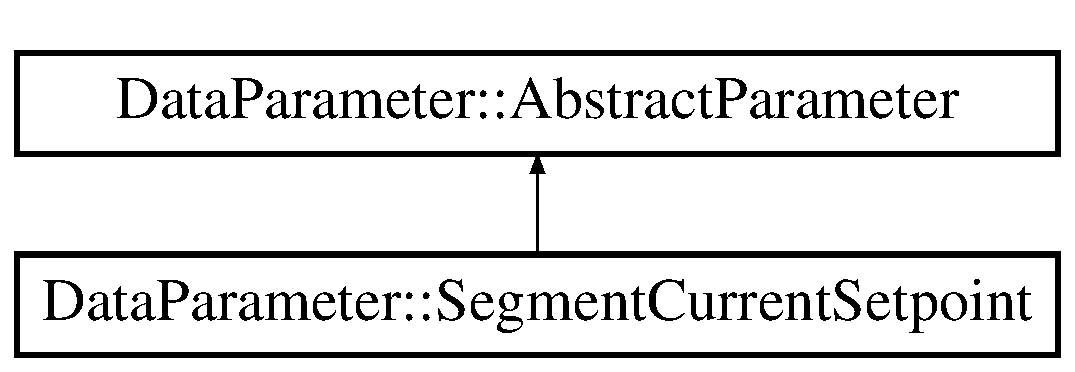
\includegraphics[height=2.000000cm]{d0/de7/class_data_parameter_1_1_segment_current_setpoint}
\end{center}
\end{figure}
\subsection*{Public Member Functions}
\begin{DoxyCompactItemize}
\item 
\textbf{ Segment\+Current\+Setpoint} (const \textbf{ Data\+::\+Segment\+Level} \&level\+Value, const \textbf{ Data\+::\+Segment\+Mode} \&level\+Mode)
\begin{DoxyCompactList}\small\item\em \doxyref{Segment\+Current\+Setpoint}{p.}{d0/de7/class_data_parameter_1_1_segment_current_setpoint}. \end{DoxyCompactList}\item 
virtual \textbf{ Data\+Parameter\+::\+Parameter\+Type} \textbf{ get\+Parameter\+Type} () const
\begin{DoxyCompactList}\small\item\em get\+Parameter\+Type \end{DoxyCompactList}\item 
virtual Q\+Byte\+Array \textbf{ get\+Byte\+Array} () const
\begin{DoxyCompactList}\small\item\em get\+Byte\+Array \end{DoxyCompactList}\item 
virtual std\+::string \textbf{ get\+Description} () const
\begin{DoxyCompactList}\small\item\em get\+Description \end{DoxyCompactList}\item 
void \textbf{ update\+Current\+Factor} (const \textbf{ Data\+::\+Current\+Factor\+Type} \&value)
\begin{DoxyCompactList}\small\item\em update\+Current\+Factor \end{DoxyCompactList}\item 
void \textbf{ update\+Prescale\+Power} (const \textbf{ Data\+::\+Segment\+V\+I\+Power} \&value)
\begin{DoxyCompactList}\small\item\em update\+Prescale\+Power \end{DoxyCompactList}\item 
void \textbf{ update\+Current\+Setpoint} (const int \&value)
\begin{DoxyCompactList}\small\item\em update\+Current\+Setpoint \end{DoxyCompactList}\end{DoxyCompactItemize}
\subsection*{Private Member Functions}
\begin{DoxyCompactItemize}
\item 
uint32\+\_\+t \textbf{ update\+Amps\+Bit\+Array} (const uint32\+\_\+t \&bit\+Array) const
\begin{DoxyCompactList}\small\item\em update\+Amps\+Bit\+Array \end{DoxyCompactList}\item 
uint32\+\_\+t \textbf{ update\+Prescale\+Bit\+Array} (const uint32\+\_\+t \&bit\+Array) const
\begin{DoxyCompactList}\small\item\em update\+Prescale\+Bit\+Array \end{DoxyCompactList}\item 
uint32\+\_\+t \textbf{ update\+Set\+Point\+Bit\+Array} (const uint32\+\_\+t \&bit\+Array) const
\begin{DoxyCompactList}\small\item\em update\+Set\+Point\+Bit\+Array \end{DoxyCompactList}\end{DoxyCompactItemize}
\subsection*{Private Attributes}
\begin{DoxyCompactItemize}
\item 
\textbf{ Data\+::\+Segment\+Level} \textbf{ level}
\begin{DoxyCompactList}\small\item\em level \end{DoxyCompactList}\item 
\textbf{ Data\+::\+Segment\+Mode} \textbf{ mode}
\begin{DoxyCompactList}\small\item\em mode \end{DoxyCompactList}\item 
\textbf{ Data\+::\+Current\+Factor\+Type} \textbf{ current\+Factor}
\begin{DoxyCompactList}\small\item\em current\+Factor \end{DoxyCompactList}\item 
\textbf{ Data\+::\+Segment\+V\+I\+Power} \textbf{ prescale}
\begin{DoxyCompactList}\small\item\em prescale \end{DoxyCompactList}\item 
int \textbf{ current}
\begin{DoxyCompactList}\small\item\em current \end{DoxyCompactList}\end{DoxyCompactItemize}
\subsection*{Additional Inherited Members}


\subsection{Detailed Description}
The \doxyref{Segment\+Current\+Setpoint}{p.}{d0/de7/class_data_parameter_1_1_segment_current_setpoint} class. 

Definition at line 22 of file segment\+\_\+current\+\_\+setpoint.\+h.



\subsection{Constructor \& Destructor Documentation}
\mbox{\label{class_data_parameter_1_1_segment_current_setpoint_accd683727753a632eacd3bb42a1f735e}} 
\index{Data\+Parameter\+::\+Segment\+Current\+Setpoint@{Data\+Parameter\+::\+Segment\+Current\+Setpoint}!Segment\+Current\+Setpoint@{Segment\+Current\+Setpoint}}
\index{Segment\+Current\+Setpoint@{Segment\+Current\+Setpoint}!Data\+Parameter\+::\+Segment\+Current\+Setpoint@{Data\+Parameter\+::\+Segment\+Current\+Setpoint}}
\subsubsection{Segment\+Current\+Setpoint()}
{\footnotesize\ttfamily Data\+Parameter\+::\+Segment\+Current\+Setpoint\+::\+Segment\+Current\+Setpoint (\begin{DoxyParamCaption}\item[{const \textbf{ Data\+::\+Segment\+Level} \&}]{level\+Value,  }\item[{const \textbf{ Data\+::\+Segment\+Mode} \&}]{level\+Mode }\end{DoxyParamCaption})}



\doxyref{Segment\+Current\+Setpoint}{p.}{d0/de7/class_data_parameter_1_1_segment_current_setpoint}. 


\begin{DoxyParams}{Parameters}
{\em level\+Value} & \\
\hline
{\em level\+Mode} & \\
\hline
\end{DoxyParams}


Definition at line 6 of file segment\+\_\+current\+\_\+setpoint.\+cpp.



\subsection{Member Function Documentation}
\mbox{\label{class_data_parameter_1_1_segment_current_setpoint_a960510acca9f82347ee21701e9aabd26}} 
\index{Data\+Parameter\+::\+Segment\+Current\+Setpoint@{Data\+Parameter\+::\+Segment\+Current\+Setpoint}!get\+Byte\+Array@{get\+Byte\+Array}}
\index{get\+Byte\+Array@{get\+Byte\+Array}!Data\+Parameter\+::\+Segment\+Current\+Setpoint@{Data\+Parameter\+::\+Segment\+Current\+Setpoint}}
\subsubsection{get\+Byte\+Array()}
{\footnotesize\ttfamily Q\+Byte\+Array Data\+Parameter\+::\+Segment\+Current\+Setpoint\+::get\+Byte\+Array (\begin{DoxyParamCaption}{ }\end{DoxyParamCaption}) const\hspace{0.3cm}{\ttfamily [virtual]}}



get\+Byte\+Array 

\begin{DoxyReturn}{Returns}

\end{DoxyReturn}


Implements \textbf{ Data\+Parameter\+::\+Abstract\+Parameter} \doxyref{}{p.}{da/dfc/class_data_parameter_1_1_abstract_parameter_aa170d4993cbcf85110dac80813050284}.



Definition at line 46 of file segment\+\_\+current\+\_\+setpoint.\+cpp.

\mbox{\label{class_data_parameter_1_1_segment_current_setpoint_a03ce6d68d5c9d3fd6792f2f55d1f875c}} 
\index{Data\+Parameter\+::\+Segment\+Current\+Setpoint@{Data\+Parameter\+::\+Segment\+Current\+Setpoint}!get\+Description@{get\+Description}}
\index{get\+Description@{get\+Description}!Data\+Parameter\+::\+Segment\+Current\+Setpoint@{Data\+Parameter\+::\+Segment\+Current\+Setpoint}}
\subsubsection{get\+Description()}
{\footnotesize\ttfamily std\+::string Data\+Parameter\+::\+Segment\+Current\+Setpoint\+::get\+Description (\begin{DoxyParamCaption}{ }\end{DoxyParamCaption}) const\hspace{0.3cm}{\ttfamily [virtual]}}



get\+Description 

\begin{DoxyReturn}{Returns}

\end{DoxyReturn}


Implements \textbf{ Data\+Parameter\+::\+Abstract\+Parameter} \doxyref{}{p.}{da/dfc/class_data_parameter_1_1_abstract_parameter_a48ad1857ea1ad5fb9ca9aceeabf82ba9}.



Definition at line 40 of file segment\+\_\+current\+\_\+setpoint.\+cpp.

\mbox{\label{class_data_parameter_1_1_segment_current_setpoint_ae4775df0c99e1b5fd21afbb612d8c02e}} 
\index{Data\+Parameter\+::\+Segment\+Current\+Setpoint@{Data\+Parameter\+::\+Segment\+Current\+Setpoint}!get\+Parameter\+Type@{get\+Parameter\+Type}}
\index{get\+Parameter\+Type@{get\+Parameter\+Type}!Data\+Parameter\+::\+Segment\+Current\+Setpoint@{Data\+Parameter\+::\+Segment\+Current\+Setpoint}}
\subsubsection{get\+Parameter\+Type()}
{\footnotesize\ttfamily \textbf{ Parameter\+Type} Data\+Parameter\+::\+Segment\+Current\+Setpoint\+::get\+Parameter\+Type (\begin{DoxyParamCaption}{ }\end{DoxyParamCaption}) const\hspace{0.3cm}{\ttfamily [virtual]}}



get\+Parameter\+Type 

\begin{DoxyReturn}{Returns}

\end{DoxyReturn}


Implements \textbf{ Data\+Parameter\+::\+Abstract\+Parameter} \doxyref{}{p.}{da/dfc/class_data_parameter_1_1_abstract_parameter_a5566a8d4357cc077dddd856569fe9bbb}.



Definition at line 35 of file segment\+\_\+current\+\_\+setpoint.\+cpp.

\mbox{\label{class_data_parameter_1_1_segment_current_setpoint_a1e05e3475a1473a86b1ae32b8ecb1979}} 
\index{Data\+Parameter\+::\+Segment\+Current\+Setpoint@{Data\+Parameter\+::\+Segment\+Current\+Setpoint}!update\+Amps\+Bit\+Array@{update\+Amps\+Bit\+Array}}
\index{update\+Amps\+Bit\+Array@{update\+Amps\+Bit\+Array}!Data\+Parameter\+::\+Segment\+Current\+Setpoint@{Data\+Parameter\+::\+Segment\+Current\+Setpoint}}
\subsubsection{update\+Amps\+Bit\+Array()}
{\footnotesize\ttfamily uint32\+\_\+t Data\+Parameter\+::\+Segment\+Current\+Setpoint\+::update\+Amps\+Bit\+Array (\begin{DoxyParamCaption}\item[{const uint32\+\_\+t \&}]{bit\+Array }\end{DoxyParamCaption}) const\hspace{0.3cm}{\ttfamily [private]}}



update\+Amps\+Bit\+Array 


\begin{DoxyParams}{Parameters}
{\em bit\+Array} & \\
\hline
\end{DoxyParams}
\begin{DoxyReturn}{Returns}

\end{DoxyReturn}


Definition at line 84 of file segment\+\_\+current\+\_\+setpoint.\+cpp.

\mbox{\label{class_data_parameter_1_1_segment_current_setpoint_a87f3dc129117151cd80862f903a61182}} 
\index{Data\+Parameter\+::\+Segment\+Current\+Setpoint@{Data\+Parameter\+::\+Segment\+Current\+Setpoint}!update\+Current\+Factor@{update\+Current\+Factor}}
\index{update\+Current\+Factor@{update\+Current\+Factor}!Data\+Parameter\+::\+Segment\+Current\+Setpoint@{Data\+Parameter\+::\+Segment\+Current\+Setpoint}}
\subsubsection{update\+Current\+Factor()}
{\footnotesize\ttfamily void Data\+Parameter\+::\+Segment\+Current\+Setpoint\+::update\+Current\+Factor (\begin{DoxyParamCaption}\item[{const \textbf{ Data\+::\+Current\+Factor\+Type} \&}]{value }\end{DoxyParamCaption})}



update\+Current\+Factor 


\begin{DoxyParams}{Parameters}
{\em value} & \\
\hline
\end{DoxyParams}


Definition at line 57 of file segment\+\_\+current\+\_\+setpoint.\+cpp.

\mbox{\label{class_data_parameter_1_1_segment_current_setpoint_a542298e27fe960fc5eeb98cb3d519686}} 
\index{Data\+Parameter\+::\+Segment\+Current\+Setpoint@{Data\+Parameter\+::\+Segment\+Current\+Setpoint}!update\+Current\+Setpoint@{update\+Current\+Setpoint}}
\index{update\+Current\+Setpoint@{update\+Current\+Setpoint}!Data\+Parameter\+::\+Segment\+Current\+Setpoint@{Data\+Parameter\+::\+Segment\+Current\+Setpoint}}
\subsubsection{update\+Current\+Setpoint()}
{\footnotesize\ttfamily void Data\+Parameter\+::\+Segment\+Current\+Setpoint\+::update\+Current\+Setpoint (\begin{DoxyParamCaption}\item[{const int \&}]{value }\end{DoxyParamCaption})}



update\+Current\+Setpoint 


\begin{DoxyParams}{Parameters}
{\em value} & \\
\hline
\end{DoxyParams}


Definition at line 67 of file segment\+\_\+current\+\_\+setpoint.\+cpp.

\mbox{\label{class_data_parameter_1_1_segment_current_setpoint_ab51310c5e47224a1209d22872c212f15}} 
\index{Data\+Parameter\+::\+Segment\+Current\+Setpoint@{Data\+Parameter\+::\+Segment\+Current\+Setpoint}!update\+Prescale\+Bit\+Array@{update\+Prescale\+Bit\+Array}}
\index{update\+Prescale\+Bit\+Array@{update\+Prescale\+Bit\+Array}!Data\+Parameter\+::\+Segment\+Current\+Setpoint@{Data\+Parameter\+::\+Segment\+Current\+Setpoint}}
\subsubsection{update\+Prescale\+Bit\+Array()}
{\footnotesize\ttfamily uint32\+\_\+t Data\+Parameter\+::\+Segment\+Current\+Setpoint\+::update\+Prescale\+Bit\+Array (\begin{DoxyParamCaption}\item[{const uint32\+\_\+t \&}]{bit\+Array }\end{DoxyParamCaption}) const\hspace{0.3cm}{\ttfamily [private]}}



update\+Prescale\+Bit\+Array 


\begin{DoxyParams}{Parameters}
{\em bit\+Array} & \\
\hline
\end{DoxyParams}
\begin{DoxyReturn}{Returns}

\end{DoxyReturn}


Definition at line 94 of file segment\+\_\+current\+\_\+setpoint.\+cpp.

\mbox{\label{class_data_parameter_1_1_segment_current_setpoint_aef9677a3298c3d56892ccaf510cb7dbf}} 
\index{Data\+Parameter\+::\+Segment\+Current\+Setpoint@{Data\+Parameter\+::\+Segment\+Current\+Setpoint}!update\+Prescale\+Power@{update\+Prescale\+Power}}
\index{update\+Prescale\+Power@{update\+Prescale\+Power}!Data\+Parameter\+::\+Segment\+Current\+Setpoint@{Data\+Parameter\+::\+Segment\+Current\+Setpoint}}
\subsubsection{update\+Prescale\+Power()}
{\footnotesize\ttfamily void Data\+Parameter\+::\+Segment\+Current\+Setpoint\+::update\+Prescale\+Power (\begin{DoxyParamCaption}\item[{const \textbf{ Data\+::\+Segment\+V\+I\+Power} \&}]{value }\end{DoxyParamCaption})}



update\+Prescale\+Power 


\begin{DoxyParams}{Parameters}
{\em value} & \\
\hline
\end{DoxyParams}


Definition at line 62 of file segment\+\_\+current\+\_\+setpoint.\+cpp.

\mbox{\label{class_data_parameter_1_1_segment_current_setpoint_a5781080dffd938d046ffa287d1153a2b}} 
\index{Data\+Parameter\+::\+Segment\+Current\+Setpoint@{Data\+Parameter\+::\+Segment\+Current\+Setpoint}!update\+Set\+Point\+Bit\+Array@{update\+Set\+Point\+Bit\+Array}}
\index{update\+Set\+Point\+Bit\+Array@{update\+Set\+Point\+Bit\+Array}!Data\+Parameter\+::\+Segment\+Current\+Setpoint@{Data\+Parameter\+::\+Segment\+Current\+Setpoint}}
\subsubsection{update\+Set\+Point\+Bit\+Array()}
{\footnotesize\ttfamily uint32\+\_\+t Data\+Parameter\+::\+Segment\+Current\+Setpoint\+::update\+Set\+Point\+Bit\+Array (\begin{DoxyParamCaption}\item[{const uint32\+\_\+t \&}]{bit\+Array }\end{DoxyParamCaption}) const\hspace{0.3cm}{\ttfamily [private]}}



update\+Set\+Point\+Bit\+Array 


\begin{DoxyParams}{Parameters}
{\em bit\+Array} & \\
\hline
\end{DoxyParams}
\begin{DoxyReturn}{Returns}

\end{DoxyReturn}


Definition at line 104 of file segment\+\_\+current\+\_\+setpoint.\+cpp.



\subsection{Member Data Documentation}
\mbox{\label{class_data_parameter_1_1_segment_current_setpoint_a0d6963358773bfd748694ee564e2b007}} 
\index{Data\+Parameter\+::\+Segment\+Current\+Setpoint@{Data\+Parameter\+::\+Segment\+Current\+Setpoint}!current@{current}}
\index{current@{current}!Data\+Parameter\+::\+Segment\+Current\+Setpoint@{Data\+Parameter\+::\+Segment\+Current\+Setpoint}}
\subsubsection{current}
{\footnotesize\ttfamily int Data\+Parameter\+::\+Segment\+Current\+Setpoint\+::current\hspace{0.3cm}{\ttfamily [private]}}



current 



Definition at line 116 of file segment\+\_\+current\+\_\+setpoint.\+h.

\mbox{\label{class_data_parameter_1_1_segment_current_setpoint_a0b2f831467b05a6331cbeb7f2294355e}} 
\index{Data\+Parameter\+::\+Segment\+Current\+Setpoint@{Data\+Parameter\+::\+Segment\+Current\+Setpoint}!current\+Factor@{current\+Factor}}
\index{current\+Factor@{current\+Factor}!Data\+Parameter\+::\+Segment\+Current\+Setpoint@{Data\+Parameter\+::\+Segment\+Current\+Setpoint}}
\subsubsection{current\+Factor}
{\footnotesize\ttfamily \textbf{ Data\+::\+Current\+Factor\+Type} Data\+Parameter\+::\+Segment\+Current\+Setpoint\+::current\+Factor\hspace{0.3cm}{\ttfamily [private]}}



current\+Factor 



Definition at line 106 of file segment\+\_\+current\+\_\+setpoint.\+h.

\mbox{\label{class_data_parameter_1_1_segment_current_setpoint_a5b8916d8c32e2e9b9f79b21788ba7219}} 
\index{Data\+Parameter\+::\+Segment\+Current\+Setpoint@{Data\+Parameter\+::\+Segment\+Current\+Setpoint}!level@{level}}
\index{level@{level}!Data\+Parameter\+::\+Segment\+Current\+Setpoint@{Data\+Parameter\+::\+Segment\+Current\+Setpoint}}
\subsubsection{level}
{\footnotesize\ttfamily \textbf{ Data\+::\+Segment\+Level} Data\+Parameter\+::\+Segment\+Current\+Setpoint\+::level\hspace{0.3cm}{\ttfamily [private]}}



level 



Definition at line 96 of file segment\+\_\+current\+\_\+setpoint.\+h.

\mbox{\label{class_data_parameter_1_1_segment_current_setpoint_a11fa94ec69645e30c94005536dc232d1}} 
\index{Data\+Parameter\+::\+Segment\+Current\+Setpoint@{Data\+Parameter\+::\+Segment\+Current\+Setpoint}!mode@{mode}}
\index{mode@{mode}!Data\+Parameter\+::\+Segment\+Current\+Setpoint@{Data\+Parameter\+::\+Segment\+Current\+Setpoint}}
\subsubsection{mode}
{\footnotesize\ttfamily \textbf{ Data\+::\+Segment\+Mode} Data\+Parameter\+::\+Segment\+Current\+Setpoint\+::mode\hspace{0.3cm}{\ttfamily [private]}}



mode 



Definition at line 101 of file segment\+\_\+current\+\_\+setpoint.\+h.

\mbox{\label{class_data_parameter_1_1_segment_current_setpoint_a0d159f49c5e3fa76874e06a881b97289}} 
\index{Data\+Parameter\+::\+Segment\+Current\+Setpoint@{Data\+Parameter\+::\+Segment\+Current\+Setpoint}!prescale@{prescale}}
\index{prescale@{prescale}!Data\+Parameter\+::\+Segment\+Current\+Setpoint@{Data\+Parameter\+::\+Segment\+Current\+Setpoint}}
\subsubsection{prescale}
{\footnotesize\ttfamily \textbf{ Data\+::\+Segment\+V\+I\+Power} Data\+Parameter\+::\+Segment\+Current\+Setpoint\+::prescale\hspace{0.3cm}{\ttfamily [private]}}



prescale 



Definition at line 111 of file segment\+\_\+current\+\_\+setpoint.\+h.



The documentation for this class was generated from the following files\+:\begin{DoxyCompactItemize}
\item 
src/library\+\_\+munk\+\_\+power\+\_\+supply/data\+\_\+registers/\textbf{ segment\+\_\+current\+\_\+setpoint.\+h}\item 
src/library\+\_\+munk\+\_\+power\+\_\+supply/data\+\_\+registers/\textbf{ segment\+\_\+current\+\_\+setpoint.\+cpp}\end{DoxyCompactItemize}

\section{Data\+Parameter\+:\+:Segment\+Time\+Data\+Detailed Class Reference}
\label{class_data_parameter_1_1_segment_time_data_detailed}\index{Data\+Parameter\+::\+Segment\+Time\+Data\+Detailed@{Data\+Parameter\+::\+Segment\+Time\+Data\+Detailed}}


The \doxyref{Segment\+Time\+Data\+Detailed}{p.}{d8/dfb/class_data_parameter_1_1_segment_time_data_detailed} class is the class that the user should implement when establishing a segments data. The data contained in here shall be mapped later on to the correct levels and establish the necessary current/voltage messages for interacting with the munk power supply.  




{\ttfamily \#include $<$segment\+\_\+time\+\_\+data\+\_\+detailed.\+h$>$}

\subsection*{Public Member Functions}
\begin{DoxyCompactItemize}
\item 
\textbf{ Segment\+Time\+Data\+Detailed} ()
\begin{DoxyCompactList}\small\item\em \doxyref{Segment\+Time\+Data\+Detailed}{p.}{d8/dfb/class_data_parameter_1_1_segment_time_data_detailed}. \end{DoxyCompactList}\item 
\textbf{ Segment\+Time\+Data\+Detailed} (const int \&voltage, const int \&current, const \textbf{ Data\+::\+Segment\+Mode} \&mode, const \textbf{ Data\+::\+Segment\+Power} \&power, const uint8\+\_\+t \&time)
\begin{DoxyCompactList}\small\item\em \doxyref{Segment\+Time\+Data\+Detailed}{p.}{d8/dfb/class_data_parameter_1_1_segment_time_data_detailed}. \end{DoxyCompactList}\item 
void \textbf{ set\+Segment\+Voltage} (const int \&voltage)
\begin{DoxyCompactList}\small\item\em set\+Segment\+Voltage \end{DoxyCompactList}\item 
void \textbf{ set\+Segment\+Current} (const int \&current)
\begin{DoxyCompactList}\small\item\em set\+Segment\+Current \end{DoxyCompactList}\item 
void \textbf{ set\+Segment\+Mode} (const \textbf{ Data\+::\+Segment\+Mode} \&mode)
\begin{DoxyCompactList}\small\item\em set\+Segment\+Mode \end{DoxyCompactList}\item 
void \textbf{ set\+Segment\+Power} (const \textbf{ Data\+::\+Segment\+Power} \&power)
\begin{DoxyCompactList}\small\item\em set\+Segment\+Power \end{DoxyCompactList}\item 
void \textbf{ set\+Time\+Value} (const uint8\+\_\+t \&time)
\begin{DoxyCompactList}\small\item\em set\+Time\+Value \end{DoxyCompactList}\item 
void \textbf{ reset\+Data} ()
\begin{DoxyCompactList}\small\item\em reset\+Data \end{DoxyCompactList}\item 
void \textbf{ update\+Data} (const \textbf{ Segment\+Time\+Data\+Detailed} \&data)
\begin{DoxyCompactList}\small\item\em update\+Data \end{DoxyCompactList}\item 
\textbf{ Data\+::\+Register\+Data\+Object} \textbf{ get\+Register\+Data\+Object} () const
\begin{DoxyCompactList}\small\item\em get\+Register\+Data\+Object \end{DoxyCompactList}\item 
\textbf{ Data\+::\+Segment\+Mode} \textbf{ get\+Segment\+Mode} () const
\begin{DoxyCompactList}\small\item\em get\+Segment\+Mode \end{DoxyCompactList}\item 
\textbf{ Data\+::\+Segment\+Power} \textbf{ get\+Segment\+Power} () const
\begin{DoxyCompactList}\small\item\em get\+Segment\+Power \end{DoxyCompactList}\item 
uint8\+\_\+t \textbf{ get\+Time\+Value} () const
\begin{DoxyCompactList}\small\item\em get\+Time\+Value \end{DoxyCompactList}\item 
void \textbf{ operator=} (const \textbf{ Segment\+Time\+Data\+Detailed} \&rhs)
\begin{DoxyCompactList}\small\item\em operator = \end{DoxyCompactList}\item 
bool \textbf{ operator==} (const \textbf{ Segment\+Time\+Data\+Detailed} \&rhs) const
\begin{DoxyCompactList}\small\item\em operator == \end{DoxyCompactList}\item 
bool \textbf{ operator!=} (const \textbf{ Segment\+Time\+Data\+Detailed} \&rhs) const
\begin{DoxyCompactList}\small\item\em operator != \end{DoxyCompactList}\end{DoxyCompactItemize}
\subsection*{Private Attributes}
\begin{DoxyCompactItemize}
\item 
\textbf{ Data\+::\+Register\+Data\+Object} \textbf{ data\+Object}
\begin{DoxyCompactList}\small\item\em data\+Object \end{DoxyCompactList}\item 
\textbf{ Data\+::\+Segment\+Mode} \textbf{ segment\+Mode}
\begin{DoxyCompactList}\small\item\em segment\+Mode \end{DoxyCompactList}\item 
\textbf{ Data\+::\+Segment\+Power} \textbf{ segment\+Power}
\begin{DoxyCompactList}\small\item\em segment\+Power \end{DoxyCompactList}\item 
uint8\+\_\+t \textbf{ time\+Value}
\begin{DoxyCompactList}\small\item\em time\+Value \end{DoxyCompactList}\end{DoxyCompactItemize}


\subsection{Detailed Description}
The \doxyref{Segment\+Time\+Data\+Detailed}{p.}{d8/dfb/class_data_parameter_1_1_segment_time_data_detailed} class is the class that the user should implement when establishing a segments data. The data contained in here shall be mapped later on to the correct levels and establish the necessary current/voltage messages for interacting with the munk power supply. 

Definition at line 17 of file segment\+\_\+time\+\_\+data\+\_\+detailed.\+h.



\subsection{Constructor \& Destructor Documentation}
\mbox{\label{class_data_parameter_1_1_segment_time_data_detailed_a32a6bf991cc7457bbb18f4b9e1aaae9e}} 
\index{Data\+Parameter\+::\+Segment\+Time\+Data\+Detailed@{Data\+Parameter\+::\+Segment\+Time\+Data\+Detailed}!Segment\+Time\+Data\+Detailed@{Segment\+Time\+Data\+Detailed}}
\index{Segment\+Time\+Data\+Detailed@{Segment\+Time\+Data\+Detailed}!Data\+Parameter\+::\+Segment\+Time\+Data\+Detailed@{Data\+Parameter\+::\+Segment\+Time\+Data\+Detailed}}
\subsubsection{Segment\+Time\+Data\+Detailed()\hspace{0.1cm}{\footnotesize\ttfamily [1/2]}}
{\footnotesize\ttfamily Data\+Parameter\+::\+Segment\+Time\+Data\+Detailed\+::\+Segment\+Time\+Data\+Detailed (\begin{DoxyParamCaption}{ }\end{DoxyParamCaption})}



\doxyref{Segment\+Time\+Data\+Detailed}{p.}{d8/dfb/class_data_parameter_1_1_segment_time_data_detailed}. 



Definition at line 5 of file segment\+\_\+time\+\_\+data\+\_\+detailed.\+cpp.

\mbox{\label{class_data_parameter_1_1_segment_time_data_detailed_a947e0ee44ce7c998be21768988aabfc6}} 
\index{Data\+Parameter\+::\+Segment\+Time\+Data\+Detailed@{Data\+Parameter\+::\+Segment\+Time\+Data\+Detailed}!Segment\+Time\+Data\+Detailed@{Segment\+Time\+Data\+Detailed}}
\index{Segment\+Time\+Data\+Detailed@{Segment\+Time\+Data\+Detailed}!Data\+Parameter\+::\+Segment\+Time\+Data\+Detailed@{Data\+Parameter\+::\+Segment\+Time\+Data\+Detailed}}
\subsubsection{Segment\+Time\+Data\+Detailed()\hspace{0.1cm}{\footnotesize\ttfamily [2/2]}}
{\footnotesize\ttfamily Data\+Parameter\+::\+Segment\+Time\+Data\+Detailed\+::\+Segment\+Time\+Data\+Detailed (\begin{DoxyParamCaption}\item[{const int \&}]{voltage,  }\item[{const int \&}]{current,  }\item[{const \textbf{ Data\+::\+Segment\+Mode} \&}]{mode,  }\item[{const \textbf{ Data\+::\+Segment\+Power} \&}]{power,  }\item[{const uint8\+\_\+t \&}]{time }\end{DoxyParamCaption})}



\doxyref{Segment\+Time\+Data\+Detailed}{p.}{d8/dfb/class_data_parameter_1_1_segment_time_data_detailed}. 


\begin{DoxyParams}{Parameters}
{\em voltage} & \\
\hline
{\em current} & \\
\hline
{\em mode} & \\
\hline
{\em power} & \\
\hline
{\em time} & \\
\hline
\end{DoxyParams}


Definition at line 11 of file segment\+\_\+time\+\_\+data\+\_\+detailed.\+cpp.



\subsection{Member Function Documentation}
\mbox{\label{class_data_parameter_1_1_segment_time_data_detailed_afce4471ec22a55f1068128240476f526}} 
\index{Data\+Parameter\+::\+Segment\+Time\+Data\+Detailed@{Data\+Parameter\+::\+Segment\+Time\+Data\+Detailed}!get\+Register\+Data\+Object@{get\+Register\+Data\+Object}}
\index{get\+Register\+Data\+Object@{get\+Register\+Data\+Object}!Data\+Parameter\+::\+Segment\+Time\+Data\+Detailed@{Data\+Parameter\+::\+Segment\+Time\+Data\+Detailed}}
\subsubsection{get\+Register\+Data\+Object()}
{\footnotesize\ttfamily \textbf{ Data\+::\+Register\+Data\+Object} Data\+Parameter\+::\+Segment\+Time\+Data\+Detailed\+::get\+Register\+Data\+Object (\begin{DoxyParamCaption}{ }\end{DoxyParamCaption}) const}



get\+Register\+Data\+Object 

\begin{DoxyReturn}{Returns}

\end{DoxyReturn}


Definition at line 66 of file segment\+\_\+time\+\_\+data\+\_\+detailed.\+cpp.

\mbox{\label{class_data_parameter_1_1_segment_time_data_detailed_a7e96479dde2a32218dad8145a0319b1c}} 
\index{Data\+Parameter\+::\+Segment\+Time\+Data\+Detailed@{Data\+Parameter\+::\+Segment\+Time\+Data\+Detailed}!get\+Segment\+Mode@{get\+Segment\+Mode}}
\index{get\+Segment\+Mode@{get\+Segment\+Mode}!Data\+Parameter\+::\+Segment\+Time\+Data\+Detailed@{Data\+Parameter\+::\+Segment\+Time\+Data\+Detailed}}
\subsubsection{get\+Segment\+Mode()}
{\footnotesize\ttfamily \textbf{ Data\+::\+Segment\+Mode} Data\+Parameter\+::\+Segment\+Time\+Data\+Detailed\+::get\+Segment\+Mode (\begin{DoxyParamCaption}{ }\end{DoxyParamCaption}) const}



get\+Segment\+Mode 

\begin{DoxyReturn}{Returns}

\end{DoxyReturn}


Definition at line 71 of file segment\+\_\+time\+\_\+data\+\_\+detailed.\+cpp.

\mbox{\label{class_data_parameter_1_1_segment_time_data_detailed_a4a76e5716ef61f6f65840306e19f5ad9}} 
\index{Data\+Parameter\+::\+Segment\+Time\+Data\+Detailed@{Data\+Parameter\+::\+Segment\+Time\+Data\+Detailed}!get\+Segment\+Power@{get\+Segment\+Power}}
\index{get\+Segment\+Power@{get\+Segment\+Power}!Data\+Parameter\+::\+Segment\+Time\+Data\+Detailed@{Data\+Parameter\+::\+Segment\+Time\+Data\+Detailed}}
\subsubsection{get\+Segment\+Power()}
{\footnotesize\ttfamily \textbf{ Data\+::\+Segment\+Power} Data\+Parameter\+::\+Segment\+Time\+Data\+Detailed\+::get\+Segment\+Power (\begin{DoxyParamCaption}{ }\end{DoxyParamCaption}) const}



get\+Segment\+Power 

\begin{DoxyReturn}{Returns}

\end{DoxyReturn}


Definition at line 76 of file segment\+\_\+time\+\_\+data\+\_\+detailed.\+cpp.

\mbox{\label{class_data_parameter_1_1_segment_time_data_detailed_a1e43fc460f6ed97389bd094b03df7f9f}} 
\index{Data\+Parameter\+::\+Segment\+Time\+Data\+Detailed@{Data\+Parameter\+::\+Segment\+Time\+Data\+Detailed}!get\+Time\+Value@{get\+Time\+Value}}
\index{get\+Time\+Value@{get\+Time\+Value}!Data\+Parameter\+::\+Segment\+Time\+Data\+Detailed@{Data\+Parameter\+::\+Segment\+Time\+Data\+Detailed}}
\subsubsection{get\+Time\+Value()}
{\footnotesize\ttfamily uint8\+\_\+t Data\+Parameter\+::\+Segment\+Time\+Data\+Detailed\+::get\+Time\+Value (\begin{DoxyParamCaption}{ }\end{DoxyParamCaption}) const}



get\+Time\+Value 

\begin{DoxyReturn}{Returns}

\end{DoxyReturn}


Definition at line 81 of file segment\+\_\+time\+\_\+data\+\_\+detailed.\+cpp.

\mbox{\label{class_data_parameter_1_1_segment_time_data_detailed_a58114f2509b2f65874b5b292703772d8}} 
\index{Data\+Parameter\+::\+Segment\+Time\+Data\+Detailed@{Data\+Parameter\+::\+Segment\+Time\+Data\+Detailed}!operator"!=@{operator"!=}}
\index{operator"!=@{operator"!=}!Data\+Parameter\+::\+Segment\+Time\+Data\+Detailed@{Data\+Parameter\+::\+Segment\+Time\+Data\+Detailed}}
\subsubsection{operator"!=()}
{\footnotesize\ttfamily bool Data\+Parameter\+::\+Segment\+Time\+Data\+Detailed\+::operator!= (\begin{DoxyParamCaption}\item[{const \textbf{ Segment\+Time\+Data\+Detailed} \&}]{rhs }\end{DoxyParamCaption}) const\hspace{0.3cm}{\ttfamily [inline]}}



operator != 


\begin{DoxyParams}{Parameters}
{\em rhs} & \\
\hline
\end{DoxyParams}
\begin{DoxyReturn}{Returns}

\end{DoxyReturn}


Definition at line 142 of file segment\+\_\+time\+\_\+data\+\_\+detailed.\+h.

\mbox{\label{class_data_parameter_1_1_segment_time_data_detailed_a0016c87158f9286ba184b7ba754358cd}} 
\index{Data\+Parameter\+::\+Segment\+Time\+Data\+Detailed@{Data\+Parameter\+::\+Segment\+Time\+Data\+Detailed}!operator=@{operator=}}
\index{operator=@{operator=}!Data\+Parameter\+::\+Segment\+Time\+Data\+Detailed@{Data\+Parameter\+::\+Segment\+Time\+Data\+Detailed}}
\subsubsection{operator=()}
{\footnotesize\ttfamily void Data\+Parameter\+::\+Segment\+Time\+Data\+Detailed\+::operator= (\begin{DoxyParamCaption}\item[{const \textbf{ Segment\+Time\+Data\+Detailed} \&}]{rhs }\end{DoxyParamCaption})\hspace{0.3cm}{\ttfamily [inline]}}



operator = 


\begin{DoxyParams}{Parameters}
{\em rhs} & \\
\hline
\end{DoxyParams}


Definition at line 107 of file segment\+\_\+time\+\_\+data\+\_\+detailed.\+h.

\mbox{\label{class_data_parameter_1_1_segment_time_data_detailed_aa0812cf3650faad79e9482d4fd8e2308}} 
\index{Data\+Parameter\+::\+Segment\+Time\+Data\+Detailed@{Data\+Parameter\+::\+Segment\+Time\+Data\+Detailed}!operator==@{operator==}}
\index{operator==@{operator==}!Data\+Parameter\+::\+Segment\+Time\+Data\+Detailed@{Data\+Parameter\+::\+Segment\+Time\+Data\+Detailed}}
\subsubsection{operator==()}
{\footnotesize\ttfamily bool Data\+Parameter\+::\+Segment\+Time\+Data\+Detailed\+::operator== (\begin{DoxyParamCaption}\item[{const \textbf{ Segment\+Time\+Data\+Detailed} \&}]{rhs }\end{DoxyParamCaption}) const\hspace{0.3cm}{\ttfamily [inline]}}



operator == 


\begin{DoxyParams}{Parameters}
{\em rhs} & \\
\hline
\end{DoxyParams}
\begin{DoxyReturn}{Returns}

\end{DoxyReturn}


Definition at line 120 of file segment\+\_\+time\+\_\+data\+\_\+detailed.\+h.

\mbox{\label{class_data_parameter_1_1_segment_time_data_detailed_a14f2c32fd145c6d24ff10b9cd9549595}} 
\index{Data\+Parameter\+::\+Segment\+Time\+Data\+Detailed@{Data\+Parameter\+::\+Segment\+Time\+Data\+Detailed}!reset\+Data@{reset\+Data}}
\index{reset\+Data@{reset\+Data}!Data\+Parameter\+::\+Segment\+Time\+Data\+Detailed@{Data\+Parameter\+::\+Segment\+Time\+Data\+Detailed}}
\subsubsection{reset\+Data()}
{\footnotesize\ttfamily void Data\+Parameter\+::\+Segment\+Time\+Data\+Detailed\+::reset\+Data (\begin{DoxyParamCaption}{ }\end{DoxyParamCaption})}



reset\+Data 



Definition at line 51 of file segment\+\_\+time\+\_\+data\+\_\+detailed.\+cpp.

\mbox{\label{class_data_parameter_1_1_segment_time_data_detailed_a472cc0978b58674b9218027c9b60414d}} 
\index{Data\+Parameter\+::\+Segment\+Time\+Data\+Detailed@{Data\+Parameter\+::\+Segment\+Time\+Data\+Detailed}!set\+Segment\+Current@{set\+Segment\+Current}}
\index{set\+Segment\+Current@{set\+Segment\+Current}!Data\+Parameter\+::\+Segment\+Time\+Data\+Detailed@{Data\+Parameter\+::\+Segment\+Time\+Data\+Detailed}}
\subsubsection{set\+Segment\+Current()}
{\footnotesize\ttfamily void Data\+Parameter\+::\+Segment\+Time\+Data\+Detailed\+::set\+Segment\+Current (\begin{DoxyParamCaption}\item[{const int \&}]{current }\end{DoxyParamCaption})}



set\+Segment\+Current 


\begin{DoxyParams}{Parameters}
{\em current} & \\
\hline
\end{DoxyParams}


Definition at line 25 of file segment\+\_\+time\+\_\+data\+\_\+detailed.\+cpp.

\mbox{\label{class_data_parameter_1_1_segment_time_data_detailed_a3390f8ec7cf989643fbe98466470c5a9}} 
\index{Data\+Parameter\+::\+Segment\+Time\+Data\+Detailed@{Data\+Parameter\+::\+Segment\+Time\+Data\+Detailed}!set\+Segment\+Mode@{set\+Segment\+Mode}}
\index{set\+Segment\+Mode@{set\+Segment\+Mode}!Data\+Parameter\+::\+Segment\+Time\+Data\+Detailed@{Data\+Parameter\+::\+Segment\+Time\+Data\+Detailed}}
\subsubsection{set\+Segment\+Mode()}
{\footnotesize\ttfamily void Data\+Parameter\+::\+Segment\+Time\+Data\+Detailed\+::set\+Segment\+Mode (\begin{DoxyParamCaption}\item[{const \textbf{ Data\+::\+Segment\+Mode} \&}]{mode }\end{DoxyParamCaption})}



set\+Segment\+Mode 


\begin{DoxyParams}{Parameters}
{\em mode} & \\
\hline
\end{DoxyParams}


Definition at line 30 of file segment\+\_\+time\+\_\+data\+\_\+detailed.\+cpp.

\mbox{\label{class_data_parameter_1_1_segment_time_data_detailed_ac17bd13a092978631b3113e88fcfe888}} 
\index{Data\+Parameter\+::\+Segment\+Time\+Data\+Detailed@{Data\+Parameter\+::\+Segment\+Time\+Data\+Detailed}!set\+Segment\+Power@{set\+Segment\+Power}}
\index{set\+Segment\+Power@{set\+Segment\+Power}!Data\+Parameter\+::\+Segment\+Time\+Data\+Detailed@{Data\+Parameter\+::\+Segment\+Time\+Data\+Detailed}}
\subsubsection{set\+Segment\+Power()}
{\footnotesize\ttfamily void Data\+Parameter\+::\+Segment\+Time\+Data\+Detailed\+::set\+Segment\+Power (\begin{DoxyParamCaption}\item[{const \textbf{ Data\+::\+Segment\+Power} \&}]{power }\end{DoxyParamCaption})}



set\+Segment\+Power 


\begin{DoxyParams}{Parameters}
{\em power} & \\
\hline
\end{DoxyParams}


Definition at line 35 of file segment\+\_\+time\+\_\+data\+\_\+detailed.\+cpp.

\mbox{\label{class_data_parameter_1_1_segment_time_data_detailed_a5cc9f392069ced2d2d415b56fbc968a4}} 
\index{Data\+Parameter\+::\+Segment\+Time\+Data\+Detailed@{Data\+Parameter\+::\+Segment\+Time\+Data\+Detailed}!set\+Segment\+Voltage@{set\+Segment\+Voltage}}
\index{set\+Segment\+Voltage@{set\+Segment\+Voltage}!Data\+Parameter\+::\+Segment\+Time\+Data\+Detailed@{Data\+Parameter\+::\+Segment\+Time\+Data\+Detailed}}
\subsubsection{set\+Segment\+Voltage()}
{\footnotesize\ttfamily void Data\+Parameter\+::\+Segment\+Time\+Data\+Detailed\+::set\+Segment\+Voltage (\begin{DoxyParamCaption}\item[{const int \&}]{voltage }\end{DoxyParamCaption})}



set\+Segment\+Voltage 


\begin{DoxyParams}{Parameters}
{\em voltage} & \\
\hline
\end{DoxyParams}


Definition at line 20 of file segment\+\_\+time\+\_\+data\+\_\+detailed.\+cpp.

\mbox{\label{class_data_parameter_1_1_segment_time_data_detailed_ac36f20ca9585272409df94fa847dce82}} 
\index{Data\+Parameter\+::\+Segment\+Time\+Data\+Detailed@{Data\+Parameter\+::\+Segment\+Time\+Data\+Detailed}!set\+Time\+Value@{set\+Time\+Value}}
\index{set\+Time\+Value@{set\+Time\+Value}!Data\+Parameter\+::\+Segment\+Time\+Data\+Detailed@{Data\+Parameter\+::\+Segment\+Time\+Data\+Detailed}}
\subsubsection{set\+Time\+Value()}
{\footnotesize\ttfamily void Data\+Parameter\+::\+Segment\+Time\+Data\+Detailed\+::set\+Time\+Value (\begin{DoxyParamCaption}\item[{const uint8\+\_\+t \&}]{time }\end{DoxyParamCaption})}



set\+Time\+Value 


\begin{DoxyParams}{Parameters}
{\em time} & \\
\hline
\end{DoxyParams}


Definition at line 40 of file segment\+\_\+time\+\_\+data\+\_\+detailed.\+cpp.

\mbox{\label{class_data_parameter_1_1_segment_time_data_detailed_afc5f514417f6cccc475a728efb27b7d3}} 
\index{Data\+Parameter\+::\+Segment\+Time\+Data\+Detailed@{Data\+Parameter\+::\+Segment\+Time\+Data\+Detailed}!update\+Data@{update\+Data}}
\index{update\+Data@{update\+Data}!Data\+Parameter\+::\+Segment\+Time\+Data\+Detailed@{Data\+Parameter\+::\+Segment\+Time\+Data\+Detailed}}
\subsubsection{update\+Data()}
{\footnotesize\ttfamily void Data\+Parameter\+::\+Segment\+Time\+Data\+Detailed\+::update\+Data (\begin{DoxyParamCaption}\item[{const \textbf{ Segment\+Time\+Data\+Detailed} \&}]{data }\end{DoxyParamCaption})}



update\+Data 


\begin{DoxyParams}{Parameters}
{\em data} & \\
\hline
\end{DoxyParams}


Definition at line 60 of file segment\+\_\+time\+\_\+data\+\_\+detailed.\+cpp.



\subsection{Member Data Documentation}
\mbox{\label{class_data_parameter_1_1_segment_time_data_detailed_ad1fb27ad23a981c1a445d8f39e2ade60}} 
\index{Data\+Parameter\+::\+Segment\+Time\+Data\+Detailed@{Data\+Parameter\+::\+Segment\+Time\+Data\+Detailed}!data\+Object@{data\+Object}}
\index{data\+Object@{data\+Object}!Data\+Parameter\+::\+Segment\+Time\+Data\+Detailed@{Data\+Parameter\+::\+Segment\+Time\+Data\+Detailed}}
\subsubsection{data\+Object}
{\footnotesize\ttfamily \textbf{ Data\+::\+Register\+Data\+Object} Data\+Parameter\+::\+Segment\+Time\+Data\+Detailed\+::data\+Object\hspace{0.3cm}{\ttfamily [private]}}



data\+Object 



Definition at line 151 of file segment\+\_\+time\+\_\+data\+\_\+detailed.\+h.

\mbox{\label{class_data_parameter_1_1_segment_time_data_detailed_a5a21366af07b902688a09610c7e3e624}} 
\index{Data\+Parameter\+::\+Segment\+Time\+Data\+Detailed@{Data\+Parameter\+::\+Segment\+Time\+Data\+Detailed}!segment\+Mode@{segment\+Mode}}
\index{segment\+Mode@{segment\+Mode}!Data\+Parameter\+::\+Segment\+Time\+Data\+Detailed@{Data\+Parameter\+::\+Segment\+Time\+Data\+Detailed}}
\subsubsection{segment\+Mode}
{\footnotesize\ttfamily \textbf{ Data\+::\+Segment\+Mode} Data\+Parameter\+::\+Segment\+Time\+Data\+Detailed\+::segment\+Mode\hspace{0.3cm}{\ttfamily [private]}}



segment\+Mode 



Definition at line 156 of file segment\+\_\+time\+\_\+data\+\_\+detailed.\+h.

\mbox{\label{class_data_parameter_1_1_segment_time_data_detailed_a33269395300e3e586a64588115c193d2}} 
\index{Data\+Parameter\+::\+Segment\+Time\+Data\+Detailed@{Data\+Parameter\+::\+Segment\+Time\+Data\+Detailed}!segment\+Power@{segment\+Power}}
\index{segment\+Power@{segment\+Power}!Data\+Parameter\+::\+Segment\+Time\+Data\+Detailed@{Data\+Parameter\+::\+Segment\+Time\+Data\+Detailed}}
\subsubsection{segment\+Power}
{\footnotesize\ttfamily \textbf{ Data\+::\+Segment\+Power} Data\+Parameter\+::\+Segment\+Time\+Data\+Detailed\+::segment\+Power\hspace{0.3cm}{\ttfamily [private]}}



segment\+Power 



Definition at line 161 of file segment\+\_\+time\+\_\+data\+\_\+detailed.\+h.

\mbox{\label{class_data_parameter_1_1_segment_time_data_detailed_aac252c69aa1798376f63b6e21f539031}} 
\index{Data\+Parameter\+::\+Segment\+Time\+Data\+Detailed@{Data\+Parameter\+::\+Segment\+Time\+Data\+Detailed}!time\+Value@{time\+Value}}
\index{time\+Value@{time\+Value}!Data\+Parameter\+::\+Segment\+Time\+Data\+Detailed@{Data\+Parameter\+::\+Segment\+Time\+Data\+Detailed}}
\subsubsection{time\+Value}
{\footnotesize\ttfamily uint8\+\_\+t Data\+Parameter\+::\+Segment\+Time\+Data\+Detailed\+::time\+Value\hspace{0.3cm}{\ttfamily [private]}}



time\+Value 



Definition at line 166 of file segment\+\_\+time\+\_\+data\+\_\+detailed.\+h.



The documentation for this class was generated from the following files\+:\begin{DoxyCompactItemize}
\item 
src/library\+\_\+munk\+\_\+power\+\_\+supply/data\+\_\+registers/\textbf{ segment\+\_\+time\+\_\+data\+\_\+detailed.\+h}\item 
src/library\+\_\+munk\+\_\+power\+\_\+supply/data\+\_\+registers/\textbf{ segment\+\_\+time\+\_\+data\+\_\+detailed.\+cpp}\end{DoxyCompactItemize}

\section{Data\+Parameter\+:\+:Segment\+Time\+Data\+General Class Reference}
\label{class_data_parameter_1_1_segment_time_data_general}\index{Data\+Parameter\+::\+Segment\+Time\+Data\+General@{Data\+Parameter\+::\+Segment\+Time\+Data\+General}}


The \doxyref{Segment\+Time\+Data\+General}{p.}{d5/dbc/class_data_parameter_1_1_segment_time_data_general} class.  




{\ttfamily \#include $<$segment\+\_\+time\+\_\+data\+\_\+general.\+h$>$}

\subsection*{Public Member Functions}
\begin{DoxyCompactItemize}
\item 
\textbf{ Segment\+Time\+Data\+General} ()
\begin{DoxyCompactList}\small\item\em \doxyref{Segment\+Time\+Data\+General}{p.}{d5/dbc/class_data_parameter_1_1_segment_time_data_general}. \end{DoxyCompactList}\item 
\textbf{ Segment\+Time\+Data\+General} (const \textbf{ Data\+::\+Segment\+Level} \&level, const \textbf{ Data\+::\+Segment\+Mode} \&mode, const \textbf{ Data\+::\+Segment\+Power} \&power, const uint8\+\_\+t \&time)
\begin{DoxyCompactList}\small\item\em \doxyref{Segment\+Time\+Data\+General}{p.}{d5/dbc/class_data_parameter_1_1_segment_time_data_general}. \end{DoxyCompactList}\item 
void \textbf{ set\+Segment\+Level} (const \textbf{ Data\+::\+Segment\+Level} \&level)
\begin{DoxyCompactList}\small\item\em set\+Segment\+Level \end{DoxyCompactList}\item 
void \textbf{ set\+Segment\+Mode} (const \textbf{ Data\+::\+Segment\+Mode} \&mode)
\begin{DoxyCompactList}\small\item\em set\+Segment\+Mode \end{DoxyCompactList}\item 
void \textbf{ set\+Segment\+Power} (const \textbf{ Data\+::\+Segment\+Power} \&power)
\begin{DoxyCompactList}\small\item\em set\+Segment\+Power \end{DoxyCompactList}\item 
void \textbf{ set\+Time\+Value} (const uint8\+\_\+t \&time)
\begin{DoxyCompactList}\small\item\em set\+Time\+Value \end{DoxyCompactList}\item 
void \textbf{ reset\+Data} ()
\begin{DoxyCompactList}\small\item\em reset\+Data \end{DoxyCompactList}\item 
void \textbf{ update\+Data} (const \textbf{ Segment\+Time\+Data\+General} \&data)
\begin{DoxyCompactList}\small\item\em update\+Data \end{DoxyCompactList}\item 
uint32\+\_\+t \textbf{ get\+Constructed\+Bit\+Array} () const
\begin{DoxyCompactList}\small\item\em get\+Constructed\+Bit\+Array \end{DoxyCompactList}\item 
void \textbf{ operator=} (const \textbf{ Segment\+Time\+Data\+General} \&rhs)
\begin{DoxyCompactList}\small\item\em operator = \end{DoxyCompactList}\item 
bool \textbf{ operator==} (const \textbf{ Segment\+Time\+Data\+General} \&rhs) const
\begin{DoxyCompactList}\small\item\em operator == \end{DoxyCompactList}\item 
bool \textbf{ operator!=} (const \textbf{ Segment\+Time\+Data\+General} \&rhs) const
\begin{DoxyCompactList}\small\item\em operator != \end{DoxyCompactList}\end{DoxyCompactItemize}
\subsection*{Private Attributes}
\begin{DoxyCompactItemize}
\item 
\textbf{ Data\+::\+Segment\+Level} \textbf{ segment\+Level}
\begin{DoxyCompactList}\small\item\em segment\+Level \end{DoxyCompactList}\item 
\textbf{ Data\+::\+Segment\+Mode} \textbf{ segment\+Mode}
\begin{DoxyCompactList}\small\item\em segment\+Mode \end{DoxyCompactList}\item 
\textbf{ Data\+::\+Segment\+Power} \textbf{ segment\+Power}
\begin{DoxyCompactList}\small\item\em segment\+Power \end{DoxyCompactList}\item 
uint8\+\_\+t \textbf{ time\+Value}
\begin{DoxyCompactList}\small\item\em time\+Value \end{DoxyCompactList}\end{DoxyCompactItemize}


\subsection{Detailed Description}
The \doxyref{Segment\+Time\+Data\+General}{p.}{d5/dbc/class_data_parameter_1_1_segment_time_data_general} class. 

Definition at line 14 of file segment\+\_\+time\+\_\+data\+\_\+general.\+h.



\subsection{Constructor \& Destructor Documentation}
\mbox{\label{class_data_parameter_1_1_segment_time_data_general_a104092e36a0af8e336836840908377dd}} 
\index{Data\+Parameter\+::\+Segment\+Time\+Data\+General@{Data\+Parameter\+::\+Segment\+Time\+Data\+General}!Segment\+Time\+Data\+General@{Segment\+Time\+Data\+General}}
\index{Segment\+Time\+Data\+General@{Segment\+Time\+Data\+General}!Data\+Parameter\+::\+Segment\+Time\+Data\+General@{Data\+Parameter\+::\+Segment\+Time\+Data\+General}}
\subsubsection{Segment\+Time\+Data\+General()\hspace{0.1cm}{\footnotesize\ttfamily [1/2]}}
{\footnotesize\ttfamily Data\+Parameter\+::\+Segment\+Time\+Data\+General\+::\+Segment\+Time\+Data\+General (\begin{DoxyParamCaption}{ }\end{DoxyParamCaption})}



\doxyref{Segment\+Time\+Data\+General}{p.}{d5/dbc/class_data_parameter_1_1_segment_time_data_general}. 



Definition at line 5 of file segment\+\_\+time\+\_\+data\+\_\+general.\+cpp.

\mbox{\label{class_data_parameter_1_1_segment_time_data_general_a0dc3e919cfc30d42959857b42eb0cd3c}} 
\index{Data\+Parameter\+::\+Segment\+Time\+Data\+General@{Data\+Parameter\+::\+Segment\+Time\+Data\+General}!Segment\+Time\+Data\+General@{Segment\+Time\+Data\+General}}
\index{Segment\+Time\+Data\+General@{Segment\+Time\+Data\+General}!Data\+Parameter\+::\+Segment\+Time\+Data\+General@{Data\+Parameter\+::\+Segment\+Time\+Data\+General}}
\subsubsection{Segment\+Time\+Data\+General()\hspace{0.1cm}{\footnotesize\ttfamily [2/2]}}
{\footnotesize\ttfamily Data\+Parameter\+::\+Segment\+Time\+Data\+General\+::\+Segment\+Time\+Data\+General (\begin{DoxyParamCaption}\item[{const \textbf{ Data\+::\+Segment\+Level} \&}]{level,  }\item[{const \textbf{ Data\+::\+Segment\+Mode} \&}]{mode,  }\item[{const \textbf{ Data\+::\+Segment\+Power} \&}]{power,  }\item[{const uint8\+\_\+t \&}]{time }\end{DoxyParamCaption})}



\doxyref{Segment\+Time\+Data\+General}{p.}{d5/dbc/class_data_parameter_1_1_segment_time_data_general}. 


\begin{DoxyParams}{Parameters}
{\em level} & \\
\hline
{\em mode} & \\
\hline
{\em power} & \\
\hline
{\em time} & \\
\hline
\end{DoxyParams}


Definition at line 11 of file segment\+\_\+time\+\_\+data\+\_\+general.\+cpp.



\subsection{Member Function Documentation}
\mbox{\label{class_data_parameter_1_1_segment_time_data_general_a70fc74f96b1f5796bee0fd4b5d085aca}} 
\index{Data\+Parameter\+::\+Segment\+Time\+Data\+General@{Data\+Parameter\+::\+Segment\+Time\+Data\+General}!get\+Constructed\+Bit\+Array@{get\+Constructed\+Bit\+Array}}
\index{get\+Constructed\+Bit\+Array@{get\+Constructed\+Bit\+Array}!Data\+Parameter\+::\+Segment\+Time\+Data\+General@{Data\+Parameter\+::\+Segment\+Time\+Data\+General}}
\subsubsection{get\+Constructed\+Bit\+Array()}
{\footnotesize\ttfamily uint32\+\_\+t Data\+Parameter\+::\+Segment\+Time\+Data\+General\+::get\+Constructed\+Bit\+Array (\begin{DoxyParamCaption}{ }\end{DoxyParamCaption}) const}



get\+Constructed\+Bit\+Array 

\begin{DoxyReturn}{Returns}

\end{DoxyReturn}


Definition at line 64 of file segment\+\_\+time\+\_\+data\+\_\+general.\+cpp.

\mbox{\label{class_data_parameter_1_1_segment_time_data_general_ad33e6d2bfcee090f0a4ab021f41e6324}} 
\index{Data\+Parameter\+::\+Segment\+Time\+Data\+General@{Data\+Parameter\+::\+Segment\+Time\+Data\+General}!operator"!=@{operator"!=}}
\index{operator"!=@{operator"!=}!Data\+Parameter\+::\+Segment\+Time\+Data\+General@{Data\+Parameter\+::\+Segment\+Time\+Data\+General}}
\subsubsection{operator"!=()}
{\footnotesize\ttfamily bool Data\+Parameter\+::\+Segment\+Time\+Data\+General\+::operator!= (\begin{DoxyParamCaption}\item[{const \textbf{ Segment\+Time\+Data\+General} \&}]{rhs }\end{DoxyParamCaption}) const\hspace{0.3cm}{\ttfamily [inline]}}



operator != 


\begin{DoxyParams}{Parameters}
{\em rhs} & \\
\hline
\end{DoxyParams}
\begin{DoxyReturn}{Returns}

\end{DoxyReturn}


Definition at line 114 of file segment\+\_\+time\+\_\+data\+\_\+general.\+h.

\mbox{\label{class_data_parameter_1_1_segment_time_data_general_a1ef02462565143e731c9178dcb4353b7}} 
\index{Data\+Parameter\+::\+Segment\+Time\+Data\+General@{Data\+Parameter\+::\+Segment\+Time\+Data\+General}!operator=@{operator=}}
\index{operator=@{operator=}!Data\+Parameter\+::\+Segment\+Time\+Data\+General@{Data\+Parameter\+::\+Segment\+Time\+Data\+General}}
\subsubsection{operator=()}
{\footnotesize\ttfamily void Data\+Parameter\+::\+Segment\+Time\+Data\+General\+::operator= (\begin{DoxyParamCaption}\item[{const \textbf{ Segment\+Time\+Data\+General} \&}]{rhs }\end{DoxyParamCaption})\hspace{0.3cm}{\ttfamily [inline]}}



operator = 


\begin{DoxyParams}{Parameters}
{\em rhs} & \\
\hline
\end{DoxyParams}


Definition at line 79 of file segment\+\_\+time\+\_\+data\+\_\+general.\+h.

\mbox{\label{class_data_parameter_1_1_segment_time_data_general_ab8f0611bd4b825930e670c9d9bcc0930}} 
\index{Data\+Parameter\+::\+Segment\+Time\+Data\+General@{Data\+Parameter\+::\+Segment\+Time\+Data\+General}!operator==@{operator==}}
\index{operator==@{operator==}!Data\+Parameter\+::\+Segment\+Time\+Data\+General@{Data\+Parameter\+::\+Segment\+Time\+Data\+General}}
\subsubsection{operator==()}
{\footnotesize\ttfamily bool Data\+Parameter\+::\+Segment\+Time\+Data\+General\+::operator== (\begin{DoxyParamCaption}\item[{const \textbf{ Segment\+Time\+Data\+General} \&}]{rhs }\end{DoxyParamCaption}) const\hspace{0.3cm}{\ttfamily [inline]}}



operator == 


\begin{DoxyParams}{Parameters}
{\em rhs} & \\
\hline
\end{DoxyParams}
\begin{DoxyReturn}{Returns}

\end{DoxyReturn}


Definition at line 92 of file segment\+\_\+time\+\_\+data\+\_\+general.\+h.

\mbox{\label{class_data_parameter_1_1_segment_time_data_general_a78b3aab1b9abd37481e5df8e959a86bb}} 
\index{Data\+Parameter\+::\+Segment\+Time\+Data\+General@{Data\+Parameter\+::\+Segment\+Time\+Data\+General}!reset\+Data@{reset\+Data}}
\index{reset\+Data@{reset\+Data}!Data\+Parameter\+::\+Segment\+Time\+Data\+General@{Data\+Parameter\+::\+Segment\+Time\+Data\+General}}
\subsubsection{reset\+Data()}
{\footnotesize\ttfamily void Data\+Parameter\+::\+Segment\+Time\+Data\+General\+::reset\+Data (\begin{DoxyParamCaption}{ }\end{DoxyParamCaption})}



reset\+Data 



Definition at line 77 of file segment\+\_\+time\+\_\+data\+\_\+general.\+cpp.

\mbox{\label{class_data_parameter_1_1_segment_time_data_general_ae9d12036dc883c17b1e707a2c610ddf9}} 
\index{Data\+Parameter\+::\+Segment\+Time\+Data\+General@{Data\+Parameter\+::\+Segment\+Time\+Data\+General}!set\+Segment\+Level@{set\+Segment\+Level}}
\index{set\+Segment\+Level@{set\+Segment\+Level}!Data\+Parameter\+::\+Segment\+Time\+Data\+General@{Data\+Parameter\+::\+Segment\+Time\+Data\+General}}
\subsubsection{set\+Segment\+Level()}
{\footnotesize\ttfamily void Data\+Parameter\+::\+Segment\+Time\+Data\+General\+::set\+Segment\+Level (\begin{DoxyParamCaption}\item[{const \textbf{ Data\+::\+Segment\+Level} \&}]{level }\end{DoxyParamCaption})}



set\+Segment\+Level 


\begin{DoxyParams}{Parameters}
{\em level} & \\
\hline
\end{DoxyParams}


Definition at line 20 of file segment\+\_\+time\+\_\+data\+\_\+general.\+cpp.

\mbox{\label{class_data_parameter_1_1_segment_time_data_general_aa0592fe8711156de9324c1959694e3b7}} 
\index{Data\+Parameter\+::\+Segment\+Time\+Data\+General@{Data\+Parameter\+::\+Segment\+Time\+Data\+General}!set\+Segment\+Mode@{set\+Segment\+Mode}}
\index{set\+Segment\+Mode@{set\+Segment\+Mode}!Data\+Parameter\+::\+Segment\+Time\+Data\+General@{Data\+Parameter\+::\+Segment\+Time\+Data\+General}}
\subsubsection{set\+Segment\+Mode()}
{\footnotesize\ttfamily void Data\+Parameter\+::\+Segment\+Time\+Data\+General\+::set\+Segment\+Mode (\begin{DoxyParamCaption}\item[{const \textbf{ Data\+::\+Segment\+Mode} \&}]{mode }\end{DoxyParamCaption})}



set\+Segment\+Mode 


\begin{DoxyParams}{Parameters}
{\em mode} & \\
\hline
\end{DoxyParams}


Definition at line 37 of file segment\+\_\+time\+\_\+data\+\_\+general.\+cpp.

\mbox{\label{class_data_parameter_1_1_segment_time_data_general_ad5f4e0355f12b00e8d50edc444c83747}} 
\index{Data\+Parameter\+::\+Segment\+Time\+Data\+General@{Data\+Parameter\+::\+Segment\+Time\+Data\+General}!set\+Segment\+Power@{set\+Segment\+Power}}
\index{set\+Segment\+Power@{set\+Segment\+Power}!Data\+Parameter\+::\+Segment\+Time\+Data\+General@{Data\+Parameter\+::\+Segment\+Time\+Data\+General}}
\subsubsection{set\+Segment\+Power()}
{\footnotesize\ttfamily void Data\+Parameter\+::\+Segment\+Time\+Data\+General\+::set\+Segment\+Power (\begin{DoxyParamCaption}\item[{const \textbf{ Data\+::\+Segment\+Power} \&}]{power }\end{DoxyParamCaption})}



set\+Segment\+Power 


\begin{DoxyParams}{Parameters}
{\em power} & \\
\hline
\end{DoxyParams}


Definition at line 48 of file segment\+\_\+time\+\_\+data\+\_\+general.\+cpp.

\mbox{\label{class_data_parameter_1_1_segment_time_data_general_a3800ca2ad3cf16cc166ee9cf0eb205ef}} 
\index{Data\+Parameter\+::\+Segment\+Time\+Data\+General@{Data\+Parameter\+::\+Segment\+Time\+Data\+General}!set\+Time\+Value@{set\+Time\+Value}}
\index{set\+Time\+Value@{set\+Time\+Value}!Data\+Parameter\+::\+Segment\+Time\+Data\+General@{Data\+Parameter\+::\+Segment\+Time\+Data\+General}}
\subsubsection{set\+Time\+Value()}
{\footnotesize\ttfamily void Data\+Parameter\+::\+Segment\+Time\+Data\+General\+::set\+Time\+Value (\begin{DoxyParamCaption}\item[{const uint8\+\_\+t \&}]{time }\end{DoxyParamCaption})}



set\+Time\+Value 


\begin{DoxyParams}{Parameters}
{\em time} & \\
\hline
\end{DoxyParams}


Definition at line 53 of file segment\+\_\+time\+\_\+data\+\_\+general.\+cpp.

\mbox{\label{class_data_parameter_1_1_segment_time_data_general_a6287e3cf3943988680f636086f945459}} 
\index{Data\+Parameter\+::\+Segment\+Time\+Data\+General@{Data\+Parameter\+::\+Segment\+Time\+Data\+General}!update\+Data@{update\+Data}}
\index{update\+Data@{update\+Data}!Data\+Parameter\+::\+Segment\+Time\+Data\+General@{Data\+Parameter\+::\+Segment\+Time\+Data\+General}}
\subsubsection{update\+Data()}
{\footnotesize\ttfamily void Data\+Parameter\+::\+Segment\+Time\+Data\+General\+::update\+Data (\begin{DoxyParamCaption}\item[{const \textbf{ Segment\+Time\+Data\+General} \&}]{data }\end{DoxyParamCaption})}



update\+Data 


\begin{DoxyParams}{Parameters}
{\em data} & \\
\hline
\end{DoxyParams}


Definition at line 85 of file segment\+\_\+time\+\_\+data\+\_\+general.\+cpp.



\subsection{Member Data Documentation}
\mbox{\label{class_data_parameter_1_1_segment_time_data_general_aeba7668ae0944910cbeae7eb1b644816}} 
\index{Data\+Parameter\+::\+Segment\+Time\+Data\+General@{Data\+Parameter\+::\+Segment\+Time\+Data\+General}!segment\+Level@{segment\+Level}}
\index{segment\+Level@{segment\+Level}!Data\+Parameter\+::\+Segment\+Time\+Data\+General@{Data\+Parameter\+::\+Segment\+Time\+Data\+General}}
\subsubsection{segment\+Level}
{\footnotesize\ttfamily \textbf{ Data\+::\+Segment\+Level} Data\+Parameter\+::\+Segment\+Time\+Data\+General\+::segment\+Level\hspace{0.3cm}{\ttfamily [private]}}



segment\+Level 



Definition at line 122 of file segment\+\_\+time\+\_\+data\+\_\+general.\+h.

\mbox{\label{class_data_parameter_1_1_segment_time_data_general_a58079e3cfb1a0e308321c37a955ab834}} 
\index{Data\+Parameter\+::\+Segment\+Time\+Data\+General@{Data\+Parameter\+::\+Segment\+Time\+Data\+General}!segment\+Mode@{segment\+Mode}}
\index{segment\+Mode@{segment\+Mode}!Data\+Parameter\+::\+Segment\+Time\+Data\+General@{Data\+Parameter\+::\+Segment\+Time\+Data\+General}}
\subsubsection{segment\+Mode}
{\footnotesize\ttfamily \textbf{ Data\+::\+Segment\+Mode} Data\+Parameter\+::\+Segment\+Time\+Data\+General\+::segment\+Mode\hspace{0.3cm}{\ttfamily [private]}}



segment\+Mode 



Definition at line 127 of file segment\+\_\+time\+\_\+data\+\_\+general.\+h.

\mbox{\label{class_data_parameter_1_1_segment_time_data_general_a43f19f66e769e5542dbd8cc447355178}} 
\index{Data\+Parameter\+::\+Segment\+Time\+Data\+General@{Data\+Parameter\+::\+Segment\+Time\+Data\+General}!segment\+Power@{segment\+Power}}
\index{segment\+Power@{segment\+Power}!Data\+Parameter\+::\+Segment\+Time\+Data\+General@{Data\+Parameter\+::\+Segment\+Time\+Data\+General}}
\subsubsection{segment\+Power}
{\footnotesize\ttfamily \textbf{ Data\+::\+Segment\+Power} Data\+Parameter\+::\+Segment\+Time\+Data\+General\+::segment\+Power\hspace{0.3cm}{\ttfamily [private]}}



segment\+Power 



Definition at line 132 of file segment\+\_\+time\+\_\+data\+\_\+general.\+h.

\mbox{\label{class_data_parameter_1_1_segment_time_data_general_a68cd8005705dfa7d542bb03e6140557b}} 
\index{Data\+Parameter\+::\+Segment\+Time\+Data\+General@{Data\+Parameter\+::\+Segment\+Time\+Data\+General}!time\+Value@{time\+Value}}
\index{time\+Value@{time\+Value}!Data\+Parameter\+::\+Segment\+Time\+Data\+General@{Data\+Parameter\+::\+Segment\+Time\+Data\+General}}
\subsubsection{time\+Value}
{\footnotesize\ttfamily uint8\+\_\+t Data\+Parameter\+::\+Segment\+Time\+Data\+General\+::time\+Value\hspace{0.3cm}{\ttfamily [private]}}



time\+Value 



Definition at line 137 of file segment\+\_\+time\+\_\+data\+\_\+general.\+h.



The documentation for this class was generated from the following files\+:\begin{DoxyCompactItemize}
\item 
src/library\+\_\+munk\+\_\+power\+\_\+supply/data\+\_\+registers/\textbf{ segment\+\_\+time\+\_\+data\+\_\+general.\+h}\item 
src/library\+\_\+munk\+\_\+power\+\_\+supply/data\+\_\+registers/\textbf{ segment\+\_\+time\+\_\+data\+\_\+general.\+cpp}\end{DoxyCompactItemize}

\section{Data\+Parameter\+:\+:Segment\+Time\+Detailed Class Reference}
\label{class_data_parameter_1_1_segment_time_detailed}\index{Data\+Parameter\+::\+Segment\+Time\+Detailed@{Data\+Parameter\+::\+Segment\+Time\+Detailed}}


The \doxyref{Segment\+Time\+Detailed}{p.}{de/d8e/class_data_parameter_1_1_segment_time_detailed} class.  




{\ttfamily \#include $<$segment\+\_\+time\+\_\+detailed.\+h$>$}

Inheritance diagram for Data\+Parameter\+:\+:Segment\+Time\+Detailed\+:\begin{figure}[H]
\begin{center}
\leavevmode
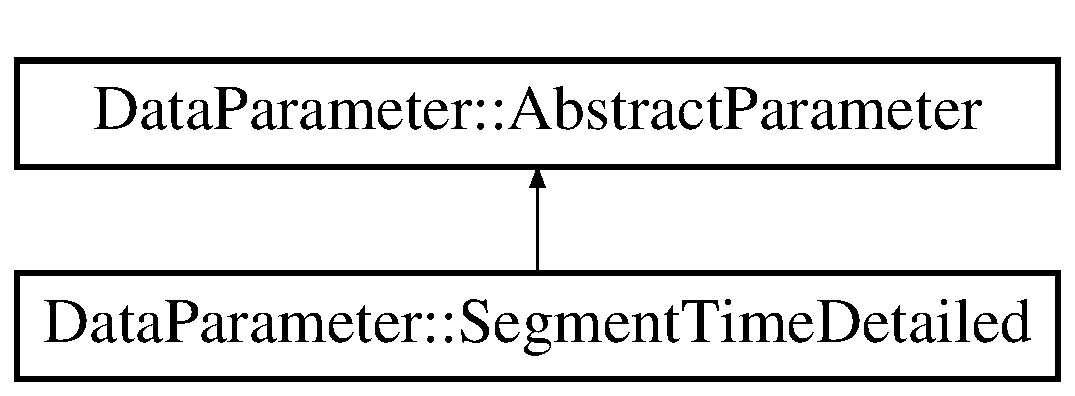
\includegraphics[height=2.000000cm]{de/d8e/class_data_parameter_1_1_segment_time_detailed}
\end{center}
\end{figure}
\subsection*{Public Member Functions}
\begin{DoxyCompactItemize}
\item 
\textbf{ Segment\+Time\+Detailed} ()
\begin{DoxyCompactList}\small\item\em \doxyref{Segment\+Time\+Detailed}{p.}{de/d8e/class_data_parameter_1_1_segment_time_detailed}. \end{DoxyCompactList}\item 
\textbf{ Segment\+Time\+Detailed} (const int \&num\+Segments)
\begin{DoxyCompactList}\small\item\em \doxyref{Segment\+Time\+Detailed}{p.}{de/d8e/class_data_parameter_1_1_segment_time_detailed}. \end{DoxyCompactList}\item 
\textbf{ Segment\+Time\+Detailed} (const \textbf{ Segment\+Time\+Detailed} \&obj)
\begin{DoxyCompactList}\small\item\em \doxyref{Segment\+Time\+Detailed}{p.}{de/d8e/class_data_parameter_1_1_segment_time_detailed}. \end{DoxyCompactList}\item 
virtual \textbf{ Data\+Parameter\+::\+Parameter\+Type} \textbf{ get\+Parameter\+Type} () const
\begin{DoxyCompactList}\small\item\em get\+Parameter\+Type \end{DoxyCompactList}\item 
virtual Q\+Byte\+Array \textbf{ get\+Byte\+Array} () const
\begin{DoxyCompactList}\small\item\em get\+Byte\+Array \end{DoxyCompactList}\item 
virtual std\+::string \textbf{ get\+Description} () const
\begin{DoxyCompactList}\small\item\em get\+Description \end{DoxyCompactList}\item 
void \textbf{ set\+Starting\+Register} (const uint8\+\_\+t \&start\+Segment)
\begin{DoxyCompactList}\small\item\em set\+Starting\+Register \end{DoxyCompactList}\item 
void \textbf{ set\+Numberof\+Sequential\+Registers} (const uint8\+\_\+t \&seq\+Segment)
\begin{DoxyCompactList}\small\item\em set\+Numberof\+Sequential\+Registers \end{DoxyCompactList}\item 
void \textbf{ append\+Register\+Data} (const \textbf{ Segment\+Time\+Data\+Detailed} \&data)
\begin{DoxyCompactList}\small\item\em append\+Register\+Data \end{DoxyCompactList}\item 
void \textbf{ update\+Register\+Data} (const int \&register\+Index, const \textbf{ Segment\+Time\+Data\+Detailed} \&data)
\begin{DoxyCompactList}\small\item\em update\+Register\+Data \end{DoxyCompactList}\item 
std\+::vector$<$ \textbf{ Data\+Parameter\+::\+Segment\+Time\+Data\+Detailed} $>$ \textbf{ get\+Register\+Data} () const
\begin{DoxyCompactList}\small\item\em get\+Register\+Data \end{DoxyCompactList}\item 
void \textbf{ initialize\+Data} ()
\begin{DoxyCompactList}\small\item\em initialize\+Data \end{DoxyCompactList}\item 
void \textbf{ operator=} (const \textbf{ Segment\+Time\+Detailed} \&rhs)
\begin{DoxyCompactList}\small\item\em operator = \end{DoxyCompactList}\item 
bool \textbf{ operator==} (const \textbf{ Segment\+Time\+Detailed} \&rhs)
\begin{DoxyCompactList}\small\item\em operator == \end{DoxyCompactList}\item 
bool \textbf{ operator!=} (const \textbf{ Segment\+Time\+Detailed} \&rhs)
\begin{DoxyCompactList}\small\item\em operator != \end{DoxyCompactList}\end{DoxyCompactItemize}
\subsection*{Private Attributes}
\begin{DoxyCompactItemize}
\item 
uint8\+\_\+t \textbf{ num\+Seq\+Segments}
\begin{DoxyCompactList}\small\item\em num\+Seq\+Segments \end{DoxyCompactList}\item 
std\+::vector$<$ \textbf{ Data\+Parameter\+::\+Segment\+Time\+Data\+Detailed} $>$ \textbf{ detailed\+Register\+Data}
\begin{DoxyCompactList}\small\item\em detailed\+Register\+Data \end{DoxyCompactList}\end{DoxyCompactItemize}
\subsection*{Additional Inherited Members}


\subsection{Detailed Description}
The \doxyref{Segment\+Time\+Detailed}{p.}{de/d8e/class_data_parameter_1_1_segment_time_detailed} class. 

Definition at line 16 of file segment\+\_\+time\+\_\+detailed.\+h.



\subsection{Constructor \& Destructor Documentation}
\mbox{\label{class_data_parameter_1_1_segment_time_detailed_a703b27f7ad99cd965018c245d5345f9a}} 
\index{Data\+Parameter\+::\+Segment\+Time\+Detailed@{Data\+Parameter\+::\+Segment\+Time\+Detailed}!Segment\+Time\+Detailed@{Segment\+Time\+Detailed}}
\index{Segment\+Time\+Detailed@{Segment\+Time\+Detailed}!Data\+Parameter\+::\+Segment\+Time\+Detailed@{Data\+Parameter\+::\+Segment\+Time\+Detailed}}
\subsubsection{Segment\+Time\+Detailed()\hspace{0.1cm}{\footnotesize\ttfamily [1/3]}}
{\footnotesize\ttfamily Data\+Parameter\+::\+Segment\+Time\+Detailed\+::\+Segment\+Time\+Detailed (\begin{DoxyParamCaption}{ }\end{DoxyParamCaption})}



\doxyref{Segment\+Time\+Detailed}{p.}{de/d8e/class_data_parameter_1_1_segment_time_detailed}. 



Definition at line 5 of file segment\+\_\+time\+\_\+detailed.\+cpp.

\mbox{\label{class_data_parameter_1_1_segment_time_detailed_a417c5ac97133098e1f77f9a1375fceb4}} 
\index{Data\+Parameter\+::\+Segment\+Time\+Detailed@{Data\+Parameter\+::\+Segment\+Time\+Detailed}!Segment\+Time\+Detailed@{Segment\+Time\+Detailed}}
\index{Segment\+Time\+Detailed@{Segment\+Time\+Detailed}!Data\+Parameter\+::\+Segment\+Time\+Detailed@{Data\+Parameter\+::\+Segment\+Time\+Detailed}}
\subsubsection{Segment\+Time\+Detailed()\hspace{0.1cm}{\footnotesize\ttfamily [2/3]}}
{\footnotesize\ttfamily Data\+Parameter\+::\+Segment\+Time\+Detailed\+::\+Segment\+Time\+Detailed (\begin{DoxyParamCaption}\item[{const int \&}]{num\+Segments }\end{DoxyParamCaption})}



\doxyref{Segment\+Time\+Detailed}{p.}{de/d8e/class_data_parameter_1_1_segment_time_detailed}. 


\begin{DoxyParams}{Parameters}
{\em num\+Segments} & \\
\hline
\end{DoxyParams}


Definition at line 11 of file segment\+\_\+time\+\_\+detailed.\+cpp.

\mbox{\label{class_data_parameter_1_1_segment_time_detailed_af172a0ead06703a93b1bff3d1875e85d}} 
\index{Data\+Parameter\+::\+Segment\+Time\+Detailed@{Data\+Parameter\+::\+Segment\+Time\+Detailed}!Segment\+Time\+Detailed@{Segment\+Time\+Detailed}}
\index{Segment\+Time\+Detailed@{Segment\+Time\+Detailed}!Data\+Parameter\+::\+Segment\+Time\+Detailed@{Data\+Parameter\+::\+Segment\+Time\+Detailed}}
\subsubsection{Segment\+Time\+Detailed()\hspace{0.1cm}{\footnotesize\ttfamily [3/3]}}
{\footnotesize\ttfamily Data\+Parameter\+::\+Segment\+Time\+Detailed\+::\+Segment\+Time\+Detailed (\begin{DoxyParamCaption}\item[{const \textbf{ Segment\+Time\+Detailed} \&}]{obj }\end{DoxyParamCaption})}



\doxyref{Segment\+Time\+Detailed}{p.}{de/d8e/class_data_parameter_1_1_segment_time_detailed}. 


\begin{DoxyParams}{Parameters}
{\em obj} & \\
\hline
\end{DoxyParams}


Definition at line 18 of file segment\+\_\+time\+\_\+detailed.\+cpp.



\subsection{Member Function Documentation}
\mbox{\label{class_data_parameter_1_1_segment_time_detailed_a9d3d73d136941f9f2564fa2505e48ffb}} 
\index{Data\+Parameter\+::\+Segment\+Time\+Detailed@{Data\+Parameter\+::\+Segment\+Time\+Detailed}!append\+Register\+Data@{append\+Register\+Data}}
\index{append\+Register\+Data@{append\+Register\+Data}!Data\+Parameter\+::\+Segment\+Time\+Detailed@{Data\+Parameter\+::\+Segment\+Time\+Detailed}}
\subsubsection{append\+Register\+Data()}
{\footnotesize\ttfamily void Data\+Parameter\+::\+Segment\+Time\+Detailed\+::append\+Register\+Data (\begin{DoxyParamCaption}\item[{const \textbf{ Segment\+Time\+Data\+Detailed} \&}]{data }\end{DoxyParamCaption})}



append\+Register\+Data 


\begin{DoxyParams}{Parameters}
{\em data} & \\
\hline
\end{DoxyParams}


Definition at line 62 of file segment\+\_\+time\+\_\+detailed.\+cpp.

\mbox{\label{class_data_parameter_1_1_segment_time_detailed_a2f55e06ca21950d3624b5d510abbec7d}} 
\index{Data\+Parameter\+::\+Segment\+Time\+Detailed@{Data\+Parameter\+::\+Segment\+Time\+Detailed}!get\+Byte\+Array@{get\+Byte\+Array}}
\index{get\+Byte\+Array@{get\+Byte\+Array}!Data\+Parameter\+::\+Segment\+Time\+Detailed@{Data\+Parameter\+::\+Segment\+Time\+Detailed}}
\subsubsection{get\+Byte\+Array()}
{\footnotesize\ttfamily Q\+Byte\+Array Data\+Parameter\+::\+Segment\+Time\+Detailed\+::get\+Byte\+Array (\begin{DoxyParamCaption}{ }\end{DoxyParamCaption}) const\hspace{0.3cm}{\ttfamily [virtual]}}



get\+Byte\+Array 

\begin{DoxyReturn}{Returns}

\end{DoxyReturn}


Implements \textbf{ Data\+Parameter\+::\+Abstract\+Parameter} \doxyref{}{p.}{da/dfc/class_data_parameter_1_1_abstract_parameter_aa170d4993cbcf85110dac80813050284}.



Definition at line 35 of file segment\+\_\+time\+\_\+detailed.\+cpp.

\mbox{\label{class_data_parameter_1_1_segment_time_detailed_a20e9b38ddc4452e2f63246aaa1c02f86}} 
\index{Data\+Parameter\+::\+Segment\+Time\+Detailed@{Data\+Parameter\+::\+Segment\+Time\+Detailed}!get\+Description@{get\+Description}}
\index{get\+Description@{get\+Description}!Data\+Parameter\+::\+Segment\+Time\+Detailed@{Data\+Parameter\+::\+Segment\+Time\+Detailed}}
\subsubsection{get\+Description()}
{\footnotesize\ttfamily std\+::string Data\+Parameter\+::\+Segment\+Time\+Detailed\+::get\+Description (\begin{DoxyParamCaption}{ }\end{DoxyParamCaption}) const\hspace{0.3cm}{\ttfamily [virtual]}}



get\+Description 

\begin{DoxyReturn}{Returns}

\end{DoxyReturn}


Implements \textbf{ Data\+Parameter\+::\+Abstract\+Parameter} \doxyref{}{p.}{da/dfc/class_data_parameter_1_1_abstract_parameter_a48ad1857ea1ad5fb9ca9aceeabf82ba9}.



Definition at line 24 of file segment\+\_\+time\+\_\+detailed.\+cpp.

\mbox{\label{class_data_parameter_1_1_segment_time_detailed_ab50e5ee5b8328d6d5b436beb6ae5a262}} 
\index{Data\+Parameter\+::\+Segment\+Time\+Detailed@{Data\+Parameter\+::\+Segment\+Time\+Detailed}!get\+Parameter\+Type@{get\+Parameter\+Type}}
\index{get\+Parameter\+Type@{get\+Parameter\+Type}!Data\+Parameter\+::\+Segment\+Time\+Detailed@{Data\+Parameter\+::\+Segment\+Time\+Detailed}}
\subsubsection{get\+Parameter\+Type()}
{\footnotesize\ttfamily \textbf{ Parameter\+Type} Data\+Parameter\+::\+Segment\+Time\+Detailed\+::get\+Parameter\+Type (\begin{DoxyParamCaption}{ }\end{DoxyParamCaption}) const\hspace{0.3cm}{\ttfamily [virtual]}}



get\+Parameter\+Type 

\begin{DoxyReturn}{Returns}

\end{DoxyReturn}


Implements \textbf{ Data\+Parameter\+::\+Abstract\+Parameter} \doxyref{}{p.}{da/dfc/class_data_parameter_1_1_abstract_parameter_a5566a8d4357cc077dddd856569fe9bbb}.



Definition at line 30 of file segment\+\_\+time\+\_\+detailed.\+cpp.

\mbox{\label{class_data_parameter_1_1_segment_time_detailed_a5ec46b19d12bf2c3b694ac18b25cfc3f}} 
\index{Data\+Parameter\+::\+Segment\+Time\+Detailed@{Data\+Parameter\+::\+Segment\+Time\+Detailed}!get\+Register\+Data@{get\+Register\+Data}}
\index{get\+Register\+Data@{get\+Register\+Data}!Data\+Parameter\+::\+Segment\+Time\+Detailed@{Data\+Parameter\+::\+Segment\+Time\+Detailed}}
\subsubsection{get\+Register\+Data()}
{\footnotesize\ttfamily std\+::vector$<$ \textbf{ Data\+Parameter\+::\+Segment\+Time\+Data\+Detailed} $>$ Data\+Parameter\+::\+Segment\+Time\+Detailed\+::get\+Register\+Data (\begin{DoxyParamCaption}{ }\end{DoxyParamCaption}) const}



get\+Register\+Data 

\begin{DoxyReturn}{Returns}

\end{DoxyReturn}


Definition at line 72 of file segment\+\_\+time\+\_\+detailed.\+cpp.

\mbox{\label{class_data_parameter_1_1_segment_time_detailed_a2cf89498541f6ee0b27db9e1a3b5374b}} 
\index{Data\+Parameter\+::\+Segment\+Time\+Detailed@{Data\+Parameter\+::\+Segment\+Time\+Detailed}!initialize\+Data@{initialize\+Data}}
\index{initialize\+Data@{initialize\+Data}!Data\+Parameter\+::\+Segment\+Time\+Detailed@{Data\+Parameter\+::\+Segment\+Time\+Detailed}}
\subsubsection{initialize\+Data()}
{\footnotesize\ttfamily void Data\+Parameter\+::\+Segment\+Time\+Detailed\+::initialize\+Data (\begin{DoxyParamCaption}{ }\end{DoxyParamCaption})}



initialize\+Data 



Definition at line 77 of file segment\+\_\+time\+\_\+detailed.\+cpp.

\mbox{\label{class_data_parameter_1_1_segment_time_detailed_a72996d214187a6f0defb0a1720e6e30e}} 
\index{Data\+Parameter\+::\+Segment\+Time\+Detailed@{Data\+Parameter\+::\+Segment\+Time\+Detailed}!operator"!=@{operator"!=}}
\index{operator"!=@{operator"!=}!Data\+Parameter\+::\+Segment\+Time\+Detailed@{Data\+Parameter\+::\+Segment\+Time\+Detailed}}
\subsubsection{operator"!=()}
{\footnotesize\ttfamily bool Data\+Parameter\+::\+Segment\+Time\+Detailed\+::operator!= (\begin{DoxyParamCaption}\item[{const \textbf{ Segment\+Time\+Detailed} \&}]{rhs }\end{DoxyParamCaption})\hspace{0.3cm}{\ttfamily [inline]}}



operator != 


\begin{DoxyParams}{Parameters}
{\em rhs} & \\
\hline
\end{DoxyParams}
\begin{DoxyReturn}{Returns}

\end{DoxyReturn}


Definition at line 130 of file segment\+\_\+time\+\_\+detailed.\+h.

\mbox{\label{class_data_parameter_1_1_segment_time_detailed_a80f096e834d2426751dc7f6f953edf1f}} 
\index{Data\+Parameter\+::\+Segment\+Time\+Detailed@{Data\+Parameter\+::\+Segment\+Time\+Detailed}!operator=@{operator=}}
\index{operator=@{operator=}!Data\+Parameter\+::\+Segment\+Time\+Detailed@{Data\+Parameter\+::\+Segment\+Time\+Detailed}}
\subsubsection{operator=()}
{\footnotesize\ttfamily void Data\+Parameter\+::\+Segment\+Time\+Detailed\+::operator= (\begin{DoxyParamCaption}\item[{const \textbf{ Segment\+Time\+Detailed} \&}]{rhs }\end{DoxyParamCaption})\hspace{0.3cm}{\ttfamily [inline]}}



operator = 


\begin{DoxyParams}{Parameters}
{\em rhs} & \\
\hline
\end{DoxyParams}


Definition at line 99 of file segment\+\_\+time\+\_\+detailed.\+h.

\mbox{\label{class_data_parameter_1_1_segment_time_detailed_aea986e83d0a4af787955d44151f2c04a}} 
\index{Data\+Parameter\+::\+Segment\+Time\+Detailed@{Data\+Parameter\+::\+Segment\+Time\+Detailed}!operator==@{operator==}}
\index{operator==@{operator==}!Data\+Parameter\+::\+Segment\+Time\+Detailed@{Data\+Parameter\+::\+Segment\+Time\+Detailed}}
\subsubsection{operator==()}
{\footnotesize\ttfamily bool Data\+Parameter\+::\+Segment\+Time\+Detailed\+::operator== (\begin{DoxyParamCaption}\item[{const \textbf{ Segment\+Time\+Detailed} \&}]{rhs }\end{DoxyParamCaption})\hspace{0.3cm}{\ttfamily [inline]}}



operator == 


\begin{DoxyParams}{Parameters}
{\em rhs} & \\
\hline
\end{DoxyParams}
\begin{DoxyReturn}{Returns}

\end{DoxyReturn}


Definition at line 111 of file segment\+\_\+time\+\_\+detailed.\+h.

\mbox{\label{class_data_parameter_1_1_segment_time_detailed_af1c750fb52e3f1e6e84dd43d61fb7c95}} 
\index{Data\+Parameter\+::\+Segment\+Time\+Detailed@{Data\+Parameter\+::\+Segment\+Time\+Detailed}!set\+Numberof\+Sequential\+Registers@{set\+Numberof\+Sequential\+Registers}}
\index{set\+Numberof\+Sequential\+Registers@{set\+Numberof\+Sequential\+Registers}!Data\+Parameter\+::\+Segment\+Time\+Detailed@{Data\+Parameter\+::\+Segment\+Time\+Detailed}}
\subsubsection{set\+Numberof\+Sequential\+Registers()}
{\footnotesize\ttfamily void Data\+Parameter\+::\+Segment\+Time\+Detailed\+::set\+Numberof\+Sequential\+Registers (\begin{DoxyParamCaption}\item[{const uint8\+\_\+t \&}]{seq\+Segment }\end{DoxyParamCaption})}



set\+Numberof\+Sequential\+Registers 


\begin{DoxyParams}{Parameters}
{\em seq\+Segment} & \\
\hline
\end{DoxyParams}


Definition at line 50 of file segment\+\_\+time\+\_\+detailed.\+cpp.

\mbox{\label{class_data_parameter_1_1_segment_time_detailed_a1d5c5fd4ee8fbc436543266378765736}} 
\index{Data\+Parameter\+::\+Segment\+Time\+Detailed@{Data\+Parameter\+::\+Segment\+Time\+Detailed}!set\+Starting\+Register@{set\+Starting\+Register}}
\index{set\+Starting\+Register@{set\+Starting\+Register}!Data\+Parameter\+::\+Segment\+Time\+Detailed@{Data\+Parameter\+::\+Segment\+Time\+Detailed}}
\subsubsection{set\+Starting\+Register()}
{\footnotesize\ttfamily void Data\+Parameter\+::\+Segment\+Time\+Detailed\+::set\+Starting\+Register (\begin{DoxyParamCaption}\item[{const uint8\+\_\+t \&}]{start\+Segment }\end{DoxyParamCaption})}



set\+Starting\+Register 


\begin{DoxyParams}{Parameters}
{\em start\+Segment} & \\
\hline
\end{DoxyParams}


Definition at line 41 of file segment\+\_\+time\+\_\+detailed.\+cpp.

\mbox{\label{class_data_parameter_1_1_segment_time_detailed_ad146332f303300e2e299e34a8fb3e010}} 
\index{Data\+Parameter\+::\+Segment\+Time\+Detailed@{Data\+Parameter\+::\+Segment\+Time\+Detailed}!update\+Register\+Data@{update\+Register\+Data}}
\index{update\+Register\+Data@{update\+Register\+Data}!Data\+Parameter\+::\+Segment\+Time\+Detailed@{Data\+Parameter\+::\+Segment\+Time\+Detailed}}
\subsubsection{update\+Register\+Data()}
{\footnotesize\ttfamily void Data\+Parameter\+::\+Segment\+Time\+Detailed\+::update\+Register\+Data (\begin{DoxyParamCaption}\item[{const int \&}]{register\+Index,  }\item[{const \textbf{ Segment\+Time\+Data\+Detailed} \&}]{data }\end{DoxyParamCaption})}



update\+Register\+Data 


\begin{DoxyParams}{Parameters}
{\em register\+Index} & \\
\hline
{\em data} & \\
\hline
\end{DoxyParams}


Definition at line 67 of file segment\+\_\+time\+\_\+detailed.\+cpp.



\subsection{Member Data Documentation}
\mbox{\label{class_data_parameter_1_1_segment_time_detailed_ab1b28d08d64344b6244763e9bcb7a091}} 
\index{Data\+Parameter\+::\+Segment\+Time\+Detailed@{Data\+Parameter\+::\+Segment\+Time\+Detailed}!detailed\+Register\+Data@{detailed\+Register\+Data}}
\index{detailed\+Register\+Data@{detailed\+Register\+Data}!Data\+Parameter\+::\+Segment\+Time\+Detailed@{Data\+Parameter\+::\+Segment\+Time\+Detailed}}
\subsubsection{detailed\+Register\+Data}
{\footnotesize\ttfamily std\+::vector$<$\textbf{ Data\+Parameter\+::\+Segment\+Time\+Data\+Detailed}$>$ Data\+Parameter\+::\+Segment\+Time\+Detailed\+::detailed\+Register\+Data\hspace{0.3cm}{\ttfamily [private]}}



detailed\+Register\+Data 



Definition at line 143 of file segment\+\_\+time\+\_\+detailed.\+h.

\mbox{\label{class_data_parameter_1_1_segment_time_detailed_adef30075c60f1b391bce88cb77aef8dd}} 
\index{Data\+Parameter\+::\+Segment\+Time\+Detailed@{Data\+Parameter\+::\+Segment\+Time\+Detailed}!num\+Seq\+Segments@{num\+Seq\+Segments}}
\index{num\+Seq\+Segments@{num\+Seq\+Segments}!Data\+Parameter\+::\+Segment\+Time\+Detailed@{Data\+Parameter\+::\+Segment\+Time\+Detailed}}
\subsubsection{num\+Seq\+Segments}
{\footnotesize\ttfamily uint8\+\_\+t Data\+Parameter\+::\+Segment\+Time\+Detailed\+::num\+Seq\+Segments\hspace{0.3cm}{\ttfamily [private]}}



num\+Seq\+Segments 



Definition at line 138 of file segment\+\_\+time\+\_\+detailed.\+h.



The documentation for this class was generated from the following files\+:\begin{DoxyCompactItemize}
\item 
src/library\+\_\+munk\+\_\+power\+\_\+supply/data\+\_\+registers/\textbf{ segment\+\_\+time\+\_\+detailed.\+h}\item 
src/library\+\_\+munk\+\_\+power\+\_\+supply/data\+\_\+registers/\textbf{ segment\+\_\+time\+\_\+detailed.\+cpp}\end{DoxyCompactItemize}

\section{Data\+Parameter\+:\+:Segment\+Time\+General Class Reference}
\label{class_data_parameter_1_1_segment_time_general}\index{Data\+Parameter\+::\+Segment\+Time\+General@{Data\+Parameter\+::\+Segment\+Time\+General}}


The \doxyref{Segment\+Time\+General}{p.}{df/dd9/class_data_parameter_1_1_segment_time_general} class.  




{\ttfamily \#include $<$segment\+\_\+time\+\_\+general.\+h$>$}

Inheritance diagram for Data\+Parameter\+:\+:Segment\+Time\+General\+:\begin{figure}[H]
\begin{center}
\leavevmode
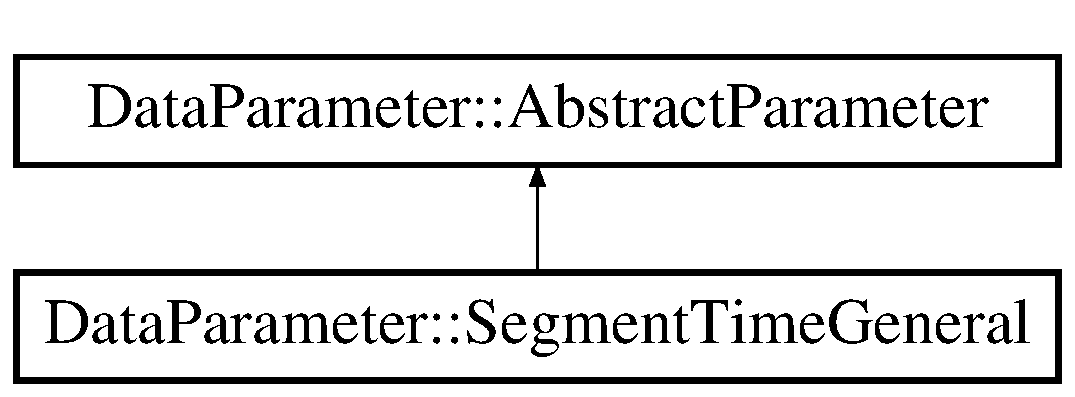
\includegraphics[height=2.000000cm]{df/dd9/class_data_parameter_1_1_segment_time_general}
\end{center}
\end{figure}
\subsection*{Public Member Functions}
\begin{DoxyCompactItemize}
\item 
\textbf{ Segment\+Time\+General} ()
\begin{DoxyCompactList}\small\item\em \doxyref{Segment\+Time\+General}{p.}{df/dd9/class_data_parameter_1_1_segment_time_general}. \end{DoxyCompactList}\item 
\textbf{ Segment\+Time\+General} (const int \&num\+Segments)
\begin{DoxyCompactList}\small\item\em \doxyref{Segment\+Time\+General}{p.}{df/dd9/class_data_parameter_1_1_segment_time_general}. \end{DoxyCompactList}\item 
\textbf{ Segment\+Time\+General} (const \textbf{ Segment\+Time\+General} \&obj)
\begin{DoxyCompactList}\small\item\em \doxyref{Segment\+Time\+General}{p.}{df/dd9/class_data_parameter_1_1_segment_time_general}. \end{DoxyCompactList}\item 
virtual \textbf{ Data\+Parameter\+::\+Parameter\+Type} \textbf{ get\+Parameter\+Type} () const
\begin{DoxyCompactList}\small\item\em get\+Parameter\+Type \end{DoxyCompactList}\item 
virtual Q\+Byte\+Array \textbf{ get\+Byte\+Array} () const
\begin{DoxyCompactList}\small\item\em get\+Byte\+Array \end{DoxyCompactList}\item 
virtual std\+::string \textbf{ get\+Description} () const
\begin{DoxyCompactList}\small\item\em get\+Description \end{DoxyCompactList}\item 
void \textbf{ set\+Starting\+Register} (const uint8\+\_\+t \&start\+Segment)
\begin{DoxyCompactList}\small\item\em set\+Starting\+Register \end{DoxyCompactList}\item 
void \textbf{ set\+Numberof\+Sequential\+Registers} (const uint8\+\_\+t \&seq\+Segment)
\begin{DoxyCompactList}\small\item\em set\+Numberof\+Sequential\+Registers \end{DoxyCompactList}\item 
void \textbf{ append\+Register\+Data} (const \textbf{ Segment\+Time\+Data\+General} \&data)
\begin{DoxyCompactList}\small\item\em append\+Register\+Data \end{DoxyCompactList}\item 
void \textbf{ update\+Register\+Data} (const int \&register\+Index, const \textbf{ Segment\+Time\+Data\+General} \&data)
\begin{DoxyCompactList}\small\item\em update\+Register\+Data \end{DoxyCompactList}\item 
void \textbf{ initialize\+Data} ()
\begin{DoxyCompactList}\small\item\em initialize\+Data \end{DoxyCompactList}\item 
void \textbf{ operator=} (const \textbf{ Segment\+Time\+General} \&rhs)
\begin{DoxyCompactList}\small\item\em operator = \end{DoxyCompactList}\item 
bool \textbf{ operator==} (const \textbf{ Segment\+Time\+General} \&rhs)
\begin{DoxyCompactList}\small\item\em operator == \end{DoxyCompactList}\item 
bool \textbf{ operator!=} (const \textbf{ Segment\+Time\+General} \&rhs)
\begin{DoxyCompactList}\small\item\em operator != \end{DoxyCompactList}\end{DoxyCompactItemize}
\subsection*{Private Attributes}
\begin{DoxyCompactItemize}
\item 
uint8\+\_\+t \textbf{ num\+Seq\+Segments}
\begin{DoxyCompactList}\small\item\em num\+Seq\+Segments \end{DoxyCompactList}\item 
std\+::vector$<$ \textbf{ Data\+Parameter\+::\+Segment\+Time\+Data\+General} $>$ \textbf{ register\+Data}
\begin{DoxyCompactList}\small\item\em register\+Data \end{DoxyCompactList}\end{DoxyCompactItemize}
\subsection*{Additional Inherited Members}


\subsection{Detailed Description}
The \doxyref{Segment\+Time\+General}{p.}{df/dd9/class_data_parameter_1_1_segment_time_general} class. 

Definition at line 19 of file segment\+\_\+time\+\_\+general.\+h.



\subsection{Constructor \& Destructor Documentation}
\mbox{\label{class_data_parameter_1_1_segment_time_general_a02685ab49eb734ffb78c030d607bfa2e}} 
\index{Data\+Parameter\+::\+Segment\+Time\+General@{Data\+Parameter\+::\+Segment\+Time\+General}!Segment\+Time\+General@{Segment\+Time\+General}}
\index{Segment\+Time\+General@{Segment\+Time\+General}!Data\+Parameter\+::\+Segment\+Time\+General@{Data\+Parameter\+::\+Segment\+Time\+General}}
\subsubsection{Segment\+Time\+General()\hspace{0.1cm}{\footnotesize\ttfamily [1/3]}}
{\footnotesize\ttfamily Data\+Parameter\+::\+Segment\+Time\+General\+::\+Segment\+Time\+General (\begin{DoxyParamCaption}{ }\end{DoxyParamCaption})}



\doxyref{Segment\+Time\+General}{p.}{df/dd9/class_data_parameter_1_1_segment_time_general}. 



Definition at line 5 of file segment\+\_\+time\+\_\+general.\+cpp.

\mbox{\label{class_data_parameter_1_1_segment_time_general_a06451651c32cfd63423145c7dc42c060}} 
\index{Data\+Parameter\+::\+Segment\+Time\+General@{Data\+Parameter\+::\+Segment\+Time\+General}!Segment\+Time\+General@{Segment\+Time\+General}}
\index{Segment\+Time\+General@{Segment\+Time\+General}!Data\+Parameter\+::\+Segment\+Time\+General@{Data\+Parameter\+::\+Segment\+Time\+General}}
\subsubsection{Segment\+Time\+General()\hspace{0.1cm}{\footnotesize\ttfamily [2/3]}}
{\footnotesize\ttfamily Data\+Parameter\+::\+Segment\+Time\+General\+::\+Segment\+Time\+General (\begin{DoxyParamCaption}\item[{const int \&}]{num\+Segments }\end{DoxyParamCaption})}



\doxyref{Segment\+Time\+General}{p.}{df/dd9/class_data_parameter_1_1_segment_time_general}. 


\begin{DoxyParams}{Parameters}
{\em num\+Segments} & \\
\hline
\end{DoxyParams}


Definition at line 11 of file segment\+\_\+time\+\_\+general.\+cpp.

\mbox{\label{class_data_parameter_1_1_segment_time_general_aa962052613165d54fef7be454f130689}} 
\index{Data\+Parameter\+::\+Segment\+Time\+General@{Data\+Parameter\+::\+Segment\+Time\+General}!Segment\+Time\+General@{Segment\+Time\+General}}
\index{Segment\+Time\+General@{Segment\+Time\+General}!Data\+Parameter\+::\+Segment\+Time\+General@{Data\+Parameter\+::\+Segment\+Time\+General}}
\subsubsection{Segment\+Time\+General()\hspace{0.1cm}{\footnotesize\ttfamily [3/3]}}
{\footnotesize\ttfamily Data\+Parameter\+::\+Segment\+Time\+General\+::\+Segment\+Time\+General (\begin{DoxyParamCaption}\item[{const \textbf{ Segment\+Time\+General} \&}]{obj }\end{DoxyParamCaption})}



\doxyref{Segment\+Time\+General}{p.}{df/dd9/class_data_parameter_1_1_segment_time_general}. 


\begin{DoxyParams}{Parameters}
{\em obj} & \\
\hline
\end{DoxyParams}


Definition at line 18 of file segment\+\_\+time\+\_\+general.\+cpp.



\subsection{Member Function Documentation}
\mbox{\label{class_data_parameter_1_1_segment_time_general_aa66ce345e7830cc559c717d43c60b1b9}} 
\index{Data\+Parameter\+::\+Segment\+Time\+General@{Data\+Parameter\+::\+Segment\+Time\+General}!append\+Register\+Data@{append\+Register\+Data}}
\index{append\+Register\+Data@{append\+Register\+Data}!Data\+Parameter\+::\+Segment\+Time\+General@{Data\+Parameter\+::\+Segment\+Time\+General}}
\subsubsection{append\+Register\+Data()}
{\footnotesize\ttfamily void Data\+Parameter\+::\+Segment\+Time\+General\+::append\+Register\+Data (\begin{DoxyParamCaption}\item[{const \textbf{ Segment\+Time\+Data\+General} \&}]{data }\end{DoxyParamCaption})}



append\+Register\+Data 


\begin{DoxyParams}{Parameters}
{\em data} & \\
\hline
\end{DoxyParams}


Definition at line 95 of file segment\+\_\+time\+\_\+general.\+cpp.

\mbox{\label{class_data_parameter_1_1_segment_time_general_a3a1ac47912c0dafd79e1ababdc856462}} 
\index{Data\+Parameter\+::\+Segment\+Time\+General@{Data\+Parameter\+::\+Segment\+Time\+General}!get\+Byte\+Array@{get\+Byte\+Array}}
\index{get\+Byte\+Array@{get\+Byte\+Array}!Data\+Parameter\+::\+Segment\+Time\+General@{Data\+Parameter\+::\+Segment\+Time\+General}}
\subsubsection{get\+Byte\+Array()}
{\footnotesize\ttfamily Q\+Byte\+Array Data\+Parameter\+::\+Segment\+Time\+General\+::get\+Byte\+Array (\begin{DoxyParamCaption}{ }\end{DoxyParamCaption}) const\hspace{0.3cm}{\ttfamily [virtual]}}



get\+Byte\+Array 

\begin{DoxyReturn}{Returns}

\end{DoxyReturn}


Implements \textbf{ Data\+Parameter\+::\+Abstract\+Parameter} \doxyref{}{p.}{da/dfc/class_data_parameter_1_1_abstract_parameter_aa170d4993cbcf85110dac80813050284}.



Definition at line 24 of file segment\+\_\+time\+\_\+general.\+cpp.

\mbox{\label{class_data_parameter_1_1_segment_time_general_a27d5b594669fdff0d6638c8d3c7d6707}} 
\index{Data\+Parameter\+::\+Segment\+Time\+General@{Data\+Parameter\+::\+Segment\+Time\+General}!get\+Description@{get\+Description}}
\index{get\+Description@{get\+Description}!Data\+Parameter\+::\+Segment\+Time\+General@{Data\+Parameter\+::\+Segment\+Time\+General}}
\subsubsection{get\+Description()}
{\footnotesize\ttfamily std\+::string Data\+Parameter\+::\+Segment\+Time\+General\+::get\+Description (\begin{DoxyParamCaption}{ }\end{DoxyParamCaption}) const\hspace{0.3cm}{\ttfamily [virtual]}}



get\+Description 

\begin{DoxyReturn}{Returns}

\end{DoxyReturn}


Implements \textbf{ Data\+Parameter\+::\+Abstract\+Parameter} \doxyref{}{p.}{da/dfc/class_data_parameter_1_1_abstract_parameter_a48ad1857ea1ad5fb9ca9aceeabf82ba9}.



Definition at line 47 of file segment\+\_\+time\+\_\+general.\+cpp.

\mbox{\label{class_data_parameter_1_1_segment_time_general_aff90789e3919a83f017c6d34c7721447}} 
\index{Data\+Parameter\+::\+Segment\+Time\+General@{Data\+Parameter\+::\+Segment\+Time\+General}!get\+Parameter\+Type@{get\+Parameter\+Type}}
\index{get\+Parameter\+Type@{get\+Parameter\+Type}!Data\+Parameter\+::\+Segment\+Time\+General@{Data\+Parameter\+::\+Segment\+Time\+General}}
\subsubsection{get\+Parameter\+Type()}
{\footnotesize\ttfamily \textbf{ Parameter\+Type} Data\+Parameter\+::\+Segment\+Time\+General\+::get\+Parameter\+Type (\begin{DoxyParamCaption}{ }\end{DoxyParamCaption}) const\hspace{0.3cm}{\ttfamily [virtual]}}



get\+Parameter\+Type 

\begin{DoxyReturn}{Returns}

\end{DoxyReturn}


Implements \textbf{ Data\+Parameter\+::\+Abstract\+Parameter} \doxyref{}{p.}{da/dfc/class_data_parameter_1_1_abstract_parameter_a5566a8d4357cc077dddd856569fe9bbb}.



Definition at line 53 of file segment\+\_\+time\+\_\+general.\+cpp.

\mbox{\label{class_data_parameter_1_1_segment_time_general_ac0ed78dea9054e315e7943b4cb176b90}} 
\index{Data\+Parameter\+::\+Segment\+Time\+General@{Data\+Parameter\+::\+Segment\+Time\+General}!initialize\+Data@{initialize\+Data}}
\index{initialize\+Data@{initialize\+Data}!Data\+Parameter\+::\+Segment\+Time\+General@{Data\+Parameter\+::\+Segment\+Time\+General}}
\subsubsection{initialize\+Data()}
{\footnotesize\ttfamily void Data\+Parameter\+::\+Segment\+Time\+General\+::initialize\+Data (\begin{DoxyParamCaption}{ }\end{DoxyParamCaption})}



initialize\+Data 



Definition at line 84 of file segment\+\_\+time\+\_\+general.\+cpp.

\mbox{\label{class_data_parameter_1_1_segment_time_general_a742bacec3f4947da76861d317fba471d}} 
\index{Data\+Parameter\+::\+Segment\+Time\+General@{Data\+Parameter\+::\+Segment\+Time\+General}!operator"!=@{operator"!=}}
\index{operator"!=@{operator"!=}!Data\+Parameter\+::\+Segment\+Time\+General@{Data\+Parameter\+::\+Segment\+Time\+General}}
\subsubsection{operator"!=()}
{\footnotesize\ttfamily bool Data\+Parameter\+::\+Segment\+Time\+General\+::operator!= (\begin{DoxyParamCaption}\item[{const \textbf{ Segment\+Time\+General} \&}]{rhs }\end{DoxyParamCaption})\hspace{0.3cm}{\ttfamily [inline]}}



operator != 


\begin{DoxyParams}{Parameters}
{\em rhs} & \\
\hline
\end{DoxyParams}
\begin{DoxyReturn}{Returns}

\end{DoxyReturn}


Definition at line 127 of file segment\+\_\+time\+\_\+general.\+h.

\mbox{\label{class_data_parameter_1_1_segment_time_general_ae188007a4d5fb045c7467454789ff408}} 
\index{Data\+Parameter\+::\+Segment\+Time\+General@{Data\+Parameter\+::\+Segment\+Time\+General}!operator=@{operator=}}
\index{operator=@{operator=}!Data\+Parameter\+::\+Segment\+Time\+General@{Data\+Parameter\+::\+Segment\+Time\+General}}
\subsubsection{operator=()}
{\footnotesize\ttfamily void Data\+Parameter\+::\+Segment\+Time\+General\+::operator= (\begin{DoxyParamCaption}\item[{const \textbf{ Segment\+Time\+General} \&}]{rhs }\end{DoxyParamCaption})\hspace{0.3cm}{\ttfamily [inline]}}



operator = 


\begin{DoxyParams}{Parameters}
{\em rhs} & \\
\hline
\end{DoxyParams}


Definition at line 96 of file segment\+\_\+time\+\_\+general.\+h.

\mbox{\label{class_data_parameter_1_1_segment_time_general_a3bc0b2f37061fd62911e4865dd2622c6}} 
\index{Data\+Parameter\+::\+Segment\+Time\+General@{Data\+Parameter\+::\+Segment\+Time\+General}!operator==@{operator==}}
\index{operator==@{operator==}!Data\+Parameter\+::\+Segment\+Time\+General@{Data\+Parameter\+::\+Segment\+Time\+General}}
\subsubsection{operator==()}
{\footnotesize\ttfamily bool Data\+Parameter\+::\+Segment\+Time\+General\+::operator== (\begin{DoxyParamCaption}\item[{const \textbf{ Segment\+Time\+General} \&}]{rhs }\end{DoxyParamCaption})\hspace{0.3cm}{\ttfamily [inline]}}



operator == 


\begin{DoxyParams}{Parameters}
{\em rhs} & \\
\hline
\end{DoxyParams}
\begin{DoxyReturn}{Returns}

\end{DoxyReturn}


Definition at line 108 of file segment\+\_\+time\+\_\+general.\+h.

\mbox{\label{class_data_parameter_1_1_segment_time_general_abba70712d662d2fd9be1a3704e274365}} 
\index{Data\+Parameter\+::\+Segment\+Time\+General@{Data\+Parameter\+::\+Segment\+Time\+General}!set\+Numberof\+Sequential\+Registers@{set\+Numberof\+Sequential\+Registers}}
\index{set\+Numberof\+Sequential\+Registers@{set\+Numberof\+Sequential\+Registers}!Data\+Parameter\+::\+Segment\+Time\+General@{Data\+Parameter\+::\+Segment\+Time\+General}}
\subsubsection{set\+Numberof\+Sequential\+Registers()}
{\footnotesize\ttfamily void Data\+Parameter\+::\+Segment\+Time\+General\+::set\+Numberof\+Sequential\+Registers (\begin{DoxyParamCaption}\item[{const uint8\+\_\+t \&}]{seq\+Segment }\end{DoxyParamCaption})}



set\+Numberof\+Sequential\+Registers 


\begin{DoxyParams}{Parameters}
{\em seq\+Segment} & \\
\hline
\end{DoxyParams}


Definition at line 67 of file segment\+\_\+time\+\_\+general.\+cpp.

\mbox{\label{class_data_parameter_1_1_segment_time_general_ab8ded1441f7019b74e9dcd3992237e6f}} 
\index{Data\+Parameter\+::\+Segment\+Time\+General@{Data\+Parameter\+::\+Segment\+Time\+General}!set\+Starting\+Register@{set\+Starting\+Register}}
\index{set\+Starting\+Register@{set\+Starting\+Register}!Data\+Parameter\+::\+Segment\+Time\+General@{Data\+Parameter\+::\+Segment\+Time\+General}}
\subsubsection{set\+Starting\+Register()}
{\footnotesize\ttfamily void Data\+Parameter\+::\+Segment\+Time\+General\+::set\+Starting\+Register (\begin{DoxyParamCaption}\item[{const uint8\+\_\+t \&}]{start\+Segment }\end{DoxyParamCaption})}



set\+Starting\+Register 


\begin{DoxyParams}{Parameters}
{\em start\+Segment} & \\
\hline
\end{DoxyParams}


Definition at line 58 of file segment\+\_\+time\+\_\+general.\+cpp.

\mbox{\label{class_data_parameter_1_1_segment_time_general_a1e55b632d5b65d6518a138f93ffc009a}} 
\index{Data\+Parameter\+::\+Segment\+Time\+General@{Data\+Parameter\+::\+Segment\+Time\+General}!update\+Register\+Data@{update\+Register\+Data}}
\index{update\+Register\+Data@{update\+Register\+Data}!Data\+Parameter\+::\+Segment\+Time\+General@{Data\+Parameter\+::\+Segment\+Time\+General}}
\subsubsection{update\+Register\+Data()}
{\footnotesize\ttfamily void Data\+Parameter\+::\+Segment\+Time\+General\+::update\+Register\+Data (\begin{DoxyParamCaption}\item[{const int \&}]{register\+Index,  }\item[{const \textbf{ Segment\+Time\+Data\+General} \&}]{data }\end{DoxyParamCaption})}



update\+Register\+Data 


\begin{DoxyParams}{Parameters}
{\em register\+Index} & \\
\hline
{\em data} & \\
\hline
\end{DoxyParams}


Definition at line 79 of file segment\+\_\+time\+\_\+general.\+cpp.



\subsection{Member Data Documentation}
\mbox{\label{class_data_parameter_1_1_segment_time_general_a06500620747b91782b201950a8ddb841}} 
\index{Data\+Parameter\+::\+Segment\+Time\+General@{Data\+Parameter\+::\+Segment\+Time\+General}!num\+Seq\+Segments@{num\+Seq\+Segments}}
\index{num\+Seq\+Segments@{num\+Seq\+Segments}!Data\+Parameter\+::\+Segment\+Time\+General@{Data\+Parameter\+::\+Segment\+Time\+General}}
\subsubsection{num\+Seq\+Segments}
{\footnotesize\ttfamily uint8\+\_\+t Data\+Parameter\+::\+Segment\+Time\+General\+::num\+Seq\+Segments\hspace{0.3cm}{\ttfamily [private]}}



num\+Seq\+Segments 



Definition at line 135 of file segment\+\_\+time\+\_\+general.\+h.

\mbox{\label{class_data_parameter_1_1_segment_time_general_a4382dc111482e11774470981813f8d2e}} 
\index{Data\+Parameter\+::\+Segment\+Time\+General@{Data\+Parameter\+::\+Segment\+Time\+General}!register\+Data@{register\+Data}}
\index{register\+Data@{register\+Data}!Data\+Parameter\+::\+Segment\+Time\+General@{Data\+Parameter\+::\+Segment\+Time\+General}}
\subsubsection{register\+Data}
{\footnotesize\ttfamily std\+::vector$<$\textbf{ Data\+Parameter\+::\+Segment\+Time\+Data\+General}$>$ Data\+Parameter\+::\+Segment\+Time\+General\+::register\+Data\hspace{0.3cm}{\ttfamily [private]}}



register\+Data 



Definition at line 140 of file segment\+\_\+time\+\_\+general.\+h.



The documentation for this class was generated from the following files\+:\begin{DoxyCompactItemize}
\item 
src/library\+\_\+munk\+\_\+power\+\_\+supply/data\+\_\+registers/\textbf{ segment\+\_\+time\+\_\+general.\+h}\item 
src/library\+\_\+munk\+\_\+power\+\_\+supply/data\+\_\+registers/\textbf{ segment\+\_\+time\+\_\+general.\+cpp}\end{DoxyCompactItemize}

\section{Data\+Parameter\+:\+:Segment\+Voltage\+Setpoint Class Reference}
\label{class_data_parameter_1_1_segment_voltage_setpoint}\index{Data\+Parameter\+::\+Segment\+Voltage\+Setpoint@{Data\+Parameter\+::\+Segment\+Voltage\+Setpoint}}


The \doxyref{Segment\+Voltage\+Setpoint}{p.}{d0/dd0/class_data_parameter_1_1_segment_voltage_setpoint} class.  




{\ttfamily \#include $<$segment\+\_\+voltage\+\_\+setpoint.\+h$>$}

Inheritance diagram for Data\+Parameter\+:\+:Segment\+Voltage\+Setpoint\+:\begin{figure}[H]
\begin{center}
\leavevmode
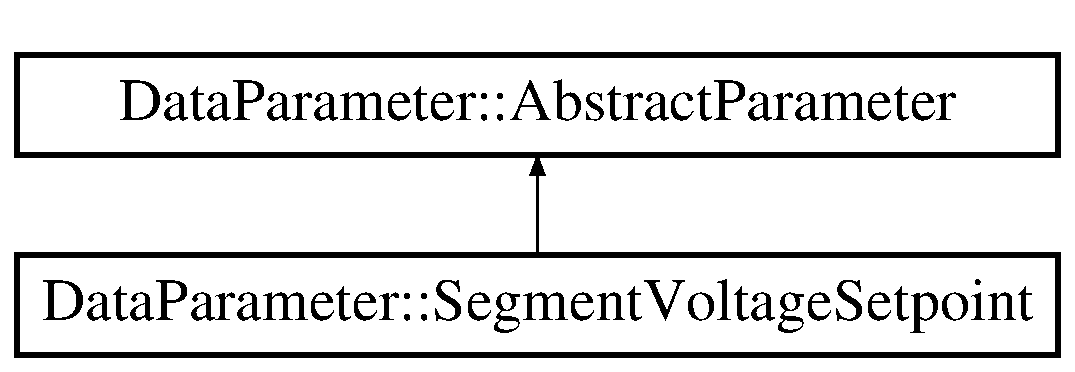
\includegraphics[height=2.000000cm]{d0/dd0/class_data_parameter_1_1_segment_voltage_setpoint}
\end{center}
\end{figure}
\subsection*{Public Member Functions}
\begin{DoxyCompactItemize}
\item 
\textbf{ Segment\+Voltage\+Setpoint} (const \textbf{ Data\+::\+Segment\+Level} \&level\+Value, const \textbf{ Data\+::\+Segment\+Mode} \&level\+Mode)
\begin{DoxyCompactList}\small\item\em \doxyref{Segment\+Voltage\+Setpoint}{p.}{d0/dd0/class_data_parameter_1_1_segment_voltage_setpoint}. \end{DoxyCompactList}\item 
virtual \textbf{ Data\+Parameter\+::\+Parameter\+Type} \textbf{ get\+Parameter\+Type} () const
\begin{DoxyCompactList}\small\item\em get\+Parameter\+Type \end{DoxyCompactList}\item 
virtual std\+::string \textbf{ get\+Description} () const
\begin{DoxyCompactList}\small\item\em get\+Description \end{DoxyCompactList}\item 
virtual Q\+Byte\+Array \textbf{ get\+Byte\+Array} () const
\begin{DoxyCompactList}\small\item\em get\+Byte\+Array \end{DoxyCompactList}\item 
void \textbf{ update\+Prescale\+Power} (const \textbf{ Data\+::\+Segment\+V\+I\+Power} \&value)
\begin{DoxyCompactList}\small\item\em update\+Prescale\+Power \end{DoxyCompactList}\item 
void \textbf{ update\+Voltage\+Setpoint} (const int \&value)
\begin{DoxyCompactList}\small\item\em update\+Voltage\+Setpoint \end{DoxyCompactList}\end{DoxyCompactItemize}
\subsection*{Private Member Functions}
\begin{DoxyCompactItemize}
\item 
uint32\+\_\+t \textbf{ update\+Prescale\+Bit\+Array} (const uint32\+\_\+t \&bit\+Array) const
\begin{DoxyCompactList}\small\item\em update\+Prescale\+Bit\+Array \end{DoxyCompactList}\item 
uint32\+\_\+t \textbf{ update\+Set\+Point\+Bit\+Array} (const uint32\+\_\+t \&bit\+Array) const
\begin{DoxyCompactList}\small\item\em update\+Set\+Point\+Bit\+Array \end{DoxyCompactList}\end{DoxyCompactItemize}
\subsection*{Private Attributes}
\begin{DoxyCompactItemize}
\item 
\textbf{ Data\+::\+Segment\+Level} \textbf{ level}
\begin{DoxyCompactList}\small\item\em level \end{DoxyCompactList}\item 
\textbf{ Data\+::\+Segment\+Mode} \textbf{ mode}
\begin{DoxyCompactList}\small\item\em mode \end{DoxyCompactList}\item 
\textbf{ Data\+::\+Segment\+V\+I\+Power} \textbf{ prescale}
\begin{DoxyCompactList}\small\item\em prescale \end{DoxyCompactList}\item 
int \textbf{ voltage}
\begin{DoxyCompactList}\small\item\em voltage \end{DoxyCompactList}\end{DoxyCompactItemize}
\subsection*{Additional Inherited Members}


\subsection{Detailed Description}
The \doxyref{Segment\+Voltage\+Setpoint}{p.}{d0/dd0/class_data_parameter_1_1_segment_voltage_setpoint} class. 

Definition at line 21 of file segment\+\_\+voltage\+\_\+setpoint.\+h.



\subsection{Constructor \& Destructor Documentation}
\mbox{\label{class_data_parameter_1_1_segment_voltage_setpoint_a9eb705f603ae3b784bc2ad46d766fa21}} 
\index{Data\+Parameter\+::\+Segment\+Voltage\+Setpoint@{Data\+Parameter\+::\+Segment\+Voltage\+Setpoint}!Segment\+Voltage\+Setpoint@{Segment\+Voltage\+Setpoint}}
\index{Segment\+Voltage\+Setpoint@{Segment\+Voltage\+Setpoint}!Data\+Parameter\+::\+Segment\+Voltage\+Setpoint@{Data\+Parameter\+::\+Segment\+Voltage\+Setpoint}}
\subsubsection{Segment\+Voltage\+Setpoint()}
{\footnotesize\ttfamily Data\+Parameter\+::\+Segment\+Voltage\+Setpoint\+::\+Segment\+Voltage\+Setpoint (\begin{DoxyParamCaption}\item[{const \textbf{ Data\+::\+Segment\+Level} \&}]{level\+Value,  }\item[{const \textbf{ Data\+::\+Segment\+Mode} \&}]{level\+Mode }\end{DoxyParamCaption})}



\doxyref{Segment\+Voltage\+Setpoint}{p.}{d0/dd0/class_data_parameter_1_1_segment_voltage_setpoint}. 

\doxyref{Segment\+Voltage\+Setpoint\+::\+Segment\+Voltage\+Setpoint}{p.}{d0/dd0/class_data_parameter_1_1_segment_voltage_setpoint_a9eb705f603ae3b784bc2ad46d766fa21}.


\begin{DoxyParams}{Parameters}
{\em level\+Value} & \\
\hline
{\em level\+Mode} & \\
\hline
\end{DoxyParams}


Definition at line 11 of file segment\+\_\+voltage\+\_\+setpoint.\+cpp.



\subsection{Member Function Documentation}
\mbox{\label{class_data_parameter_1_1_segment_voltage_setpoint_ad235d797a7a6f02096ad8dd432ee57f7}} 
\index{Data\+Parameter\+::\+Segment\+Voltage\+Setpoint@{Data\+Parameter\+::\+Segment\+Voltage\+Setpoint}!get\+Byte\+Array@{get\+Byte\+Array}}
\index{get\+Byte\+Array@{get\+Byte\+Array}!Data\+Parameter\+::\+Segment\+Voltage\+Setpoint@{Data\+Parameter\+::\+Segment\+Voltage\+Setpoint}}
\subsubsection{get\+Byte\+Array()}
{\footnotesize\ttfamily Q\+Byte\+Array Data\+Parameter\+::\+Segment\+Voltage\+Setpoint\+::get\+Byte\+Array (\begin{DoxyParamCaption}{ }\end{DoxyParamCaption}) const\hspace{0.3cm}{\ttfamily [virtual]}}



get\+Byte\+Array 

\begin{DoxyReturn}{Returns}

\end{DoxyReturn}


Implements \textbf{ Data\+Parameter\+::\+Abstract\+Parameter} \doxyref{}{p.}{da/dfc/class_data_parameter_1_1_abstract_parameter_aa170d4993cbcf85110dac80813050284}.



Definition at line 50 of file segment\+\_\+voltage\+\_\+setpoint.\+cpp.

\mbox{\label{class_data_parameter_1_1_segment_voltage_setpoint_acabde393bbee6dd5abe4c3d682fc2ee5}} 
\index{Data\+Parameter\+::\+Segment\+Voltage\+Setpoint@{Data\+Parameter\+::\+Segment\+Voltage\+Setpoint}!get\+Description@{get\+Description}}
\index{get\+Description@{get\+Description}!Data\+Parameter\+::\+Segment\+Voltage\+Setpoint@{Data\+Parameter\+::\+Segment\+Voltage\+Setpoint}}
\subsubsection{get\+Description()}
{\footnotesize\ttfamily std\+::string Data\+Parameter\+::\+Segment\+Voltage\+Setpoint\+::get\+Description (\begin{DoxyParamCaption}{ }\end{DoxyParamCaption}) const\hspace{0.3cm}{\ttfamily [virtual]}}



get\+Description 

\begin{DoxyReturn}{Returns}

\end{DoxyReturn}


Implements \textbf{ Data\+Parameter\+::\+Abstract\+Parameter} \doxyref{}{p.}{da/dfc/class_data_parameter_1_1_abstract_parameter_a48ad1857ea1ad5fb9ca9aceeabf82ba9}.



Definition at line 44 of file segment\+\_\+voltage\+\_\+setpoint.\+cpp.

\mbox{\label{class_data_parameter_1_1_segment_voltage_setpoint_aa94a5c65dade8f499b3781d8401f2ddd}} 
\index{Data\+Parameter\+::\+Segment\+Voltage\+Setpoint@{Data\+Parameter\+::\+Segment\+Voltage\+Setpoint}!get\+Parameter\+Type@{get\+Parameter\+Type}}
\index{get\+Parameter\+Type@{get\+Parameter\+Type}!Data\+Parameter\+::\+Segment\+Voltage\+Setpoint@{Data\+Parameter\+::\+Segment\+Voltage\+Setpoint}}
\subsubsection{get\+Parameter\+Type()}
{\footnotesize\ttfamily \textbf{ Parameter\+Type} Data\+Parameter\+::\+Segment\+Voltage\+Setpoint\+::get\+Parameter\+Type (\begin{DoxyParamCaption}{ }\end{DoxyParamCaption}) const\hspace{0.3cm}{\ttfamily [virtual]}}



get\+Parameter\+Type 

\begin{DoxyReturn}{Returns}

\end{DoxyReturn}


Implements \textbf{ Data\+Parameter\+::\+Abstract\+Parameter} \doxyref{}{p.}{da/dfc/class_data_parameter_1_1_abstract_parameter_a5566a8d4357cc077dddd856569fe9bbb}.



Definition at line 39 of file segment\+\_\+voltage\+\_\+setpoint.\+cpp.

\mbox{\label{class_data_parameter_1_1_segment_voltage_setpoint_a9fd1c813a1f0cf4fa36bf4c0018b0b3f}} 
\index{Data\+Parameter\+::\+Segment\+Voltage\+Setpoint@{Data\+Parameter\+::\+Segment\+Voltage\+Setpoint}!update\+Prescale\+Bit\+Array@{update\+Prescale\+Bit\+Array}}
\index{update\+Prescale\+Bit\+Array@{update\+Prescale\+Bit\+Array}!Data\+Parameter\+::\+Segment\+Voltage\+Setpoint@{Data\+Parameter\+::\+Segment\+Voltage\+Setpoint}}
\subsubsection{update\+Prescale\+Bit\+Array()}
{\footnotesize\ttfamily uint32\+\_\+t Data\+Parameter\+::\+Segment\+Voltage\+Setpoint\+::update\+Prescale\+Bit\+Array (\begin{DoxyParamCaption}\item[{const uint32\+\_\+t \&}]{bit\+Array }\end{DoxyParamCaption}) const\hspace{0.3cm}{\ttfamily [private]}}



update\+Prescale\+Bit\+Array 


\begin{DoxyParams}{Parameters}
{\em bit\+Array} & \\
\hline
\end{DoxyParams}
\begin{DoxyReturn}{Returns}

\end{DoxyReturn}


Definition at line 82 of file segment\+\_\+voltage\+\_\+setpoint.\+cpp.

\mbox{\label{class_data_parameter_1_1_segment_voltage_setpoint_ae2dfa3d0086eafa9496508cc32577302}} 
\index{Data\+Parameter\+::\+Segment\+Voltage\+Setpoint@{Data\+Parameter\+::\+Segment\+Voltage\+Setpoint}!update\+Prescale\+Power@{update\+Prescale\+Power}}
\index{update\+Prescale\+Power@{update\+Prescale\+Power}!Data\+Parameter\+::\+Segment\+Voltage\+Setpoint@{Data\+Parameter\+::\+Segment\+Voltage\+Setpoint}}
\subsubsection{update\+Prescale\+Power()}
{\footnotesize\ttfamily void Data\+Parameter\+::\+Segment\+Voltage\+Setpoint\+::update\+Prescale\+Power (\begin{DoxyParamCaption}\item[{const \textbf{ Data\+::\+Segment\+V\+I\+Power} \&}]{value }\end{DoxyParamCaption})}



update\+Prescale\+Power 


\begin{DoxyParams}{Parameters}
{\em value} & \\
\hline
\end{DoxyParams}


Definition at line 60 of file segment\+\_\+voltage\+\_\+setpoint.\+cpp.

\mbox{\label{class_data_parameter_1_1_segment_voltage_setpoint_aa1aea2b0296423784180c33bca5b8645}} 
\index{Data\+Parameter\+::\+Segment\+Voltage\+Setpoint@{Data\+Parameter\+::\+Segment\+Voltage\+Setpoint}!update\+Set\+Point\+Bit\+Array@{update\+Set\+Point\+Bit\+Array}}
\index{update\+Set\+Point\+Bit\+Array@{update\+Set\+Point\+Bit\+Array}!Data\+Parameter\+::\+Segment\+Voltage\+Setpoint@{Data\+Parameter\+::\+Segment\+Voltage\+Setpoint}}
\subsubsection{update\+Set\+Point\+Bit\+Array()}
{\footnotesize\ttfamily uint32\+\_\+t Data\+Parameter\+::\+Segment\+Voltage\+Setpoint\+::update\+Set\+Point\+Bit\+Array (\begin{DoxyParamCaption}\item[{const uint32\+\_\+t \&}]{bit\+Array }\end{DoxyParamCaption}) const\hspace{0.3cm}{\ttfamily [private]}}



update\+Set\+Point\+Bit\+Array 


\begin{DoxyParams}{Parameters}
{\em bit\+Array} & \\
\hline
\end{DoxyParams}
\begin{DoxyReturn}{Returns}

\end{DoxyReturn}


Definition at line 92 of file segment\+\_\+voltage\+\_\+setpoint.\+cpp.

\mbox{\label{class_data_parameter_1_1_segment_voltage_setpoint_ad20a85ce851ef59e016ff5c0b2f63aee}} 
\index{Data\+Parameter\+::\+Segment\+Voltage\+Setpoint@{Data\+Parameter\+::\+Segment\+Voltage\+Setpoint}!update\+Voltage\+Setpoint@{update\+Voltage\+Setpoint}}
\index{update\+Voltage\+Setpoint@{update\+Voltage\+Setpoint}!Data\+Parameter\+::\+Segment\+Voltage\+Setpoint@{Data\+Parameter\+::\+Segment\+Voltage\+Setpoint}}
\subsubsection{update\+Voltage\+Setpoint()}
{\footnotesize\ttfamily void Data\+Parameter\+::\+Segment\+Voltage\+Setpoint\+::update\+Voltage\+Setpoint (\begin{DoxyParamCaption}\item[{const int \&}]{value }\end{DoxyParamCaption})}



update\+Voltage\+Setpoint 


\begin{DoxyParams}{Parameters}
{\em value} & \\
\hline
\end{DoxyParams}


Definition at line 65 of file segment\+\_\+voltage\+\_\+setpoint.\+cpp.



\subsection{Member Data Documentation}
\mbox{\label{class_data_parameter_1_1_segment_voltage_setpoint_a8082cfb574dc3959bedfcce8e6d2dd63}} 
\index{Data\+Parameter\+::\+Segment\+Voltage\+Setpoint@{Data\+Parameter\+::\+Segment\+Voltage\+Setpoint}!level@{level}}
\index{level@{level}!Data\+Parameter\+::\+Segment\+Voltage\+Setpoint@{Data\+Parameter\+::\+Segment\+Voltage\+Setpoint}}
\subsubsection{level}
{\footnotesize\ttfamily \textbf{ Data\+::\+Segment\+Level} Data\+Parameter\+::\+Segment\+Voltage\+Setpoint\+::level\hspace{0.3cm}{\ttfamily [private]}}



level 



Definition at line 84 of file segment\+\_\+voltage\+\_\+setpoint.\+h.

\mbox{\label{class_data_parameter_1_1_segment_voltage_setpoint_a0a14845c3e651c63aa4a22dc3ca5d863}} 
\index{Data\+Parameter\+::\+Segment\+Voltage\+Setpoint@{Data\+Parameter\+::\+Segment\+Voltage\+Setpoint}!mode@{mode}}
\index{mode@{mode}!Data\+Parameter\+::\+Segment\+Voltage\+Setpoint@{Data\+Parameter\+::\+Segment\+Voltage\+Setpoint}}
\subsubsection{mode}
{\footnotesize\ttfamily \textbf{ Data\+::\+Segment\+Mode} Data\+Parameter\+::\+Segment\+Voltage\+Setpoint\+::mode\hspace{0.3cm}{\ttfamily [private]}}



mode 



Definition at line 89 of file segment\+\_\+voltage\+\_\+setpoint.\+h.

\mbox{\label{class_data_parameter_1_1_segment_voltage_setpoint_a24cbc6343b200251b608f7edd1d45136}} 
\index{Data\+Parameter\+::\+Segment\+Voltage\+Setpoint@{Data\+Parameter\+::\+Segment\+Voltage\+Setpoint}!prescale@{prescale}}
\index{prescale@{prescale}!Data\+Parameter\+::\+Segment\+Voltage\+Setpoint@{Data\+Parameter\+::\+Segment\+Voltage\+Setpoint}}
\subsubsection{prescale}
{\footnotesize\ttfamily \textbf{ Data\+::\+Segment\+V\+I\+Power} Data\+Parameter\+::\+Segment\+Voltage\+Setpoint\+::prescale\hspace{0.3cm}{\ttfamily [private]}}



prescale 



Definition at line 94 of file segment\+\_\+voltage\+\_\+setpoint.\+h.

\mbox{\label{class_data_parameter_1_1_segment_voltage_setpoint_a34ff944292110924f295349c3f14a414}} 
\index{Data\+Parameter\+::\+Segment\+Voltage\+Setpoint@{Data\+Parameter\+::\+Segment\+Voltage\+Setpoint}!voltage@{voltage}}
\index{voltage@{voltage}!Data\+Parameter\+::\+Segment\+Voltage\+Setpoint@{Data\+Parameter\+::\+Segment\+Voltage\+Setpoint}}
\subsubsection{voltage}
{\footnotesize\ttfamily int Data\+Parameter\+::\+Segment\+Voltage\+Setpoint\+::voltage\hspace{0.3cm}{\ttfamily [private]}}



voltage 



Definition at line 99 of file segment\+\_\+voltage\+\_\+setpoint.\+h.



The documentation for this class was generated from the following files\+:\begin{DoxyCompactItemize}
\item 
src/library\+\_\+munk\+\_\+power\+\_\+supply/data\+\_\+registers/\textbf{ segment\+\_\+voltage\+\_\+setpoint.\+h}\item 
src/library\+\_\+munk\+\_\+power\+\_\+supply/data\+\_\+registers/\textbf{ segment\+\_\+voltage\+\_\+setpoint.\+cpp}\end{DoxyCompactItemize}

\section{Ui\+\_\+\+Main\+Window Class Reference}
\label{class_ui___main_window}\index{Ui\+\_\+\+Main\+Window@{Ui\+\_\+\+Main\+Window}}


{\ttfamily \#include $<$ui\+\_\+mainwindow.\+h$>$}

Inheritance diagram for Ui\+\_\+\+Main\+Window\+:\begin{figure}[H]
\begin{center}
\leavevmode
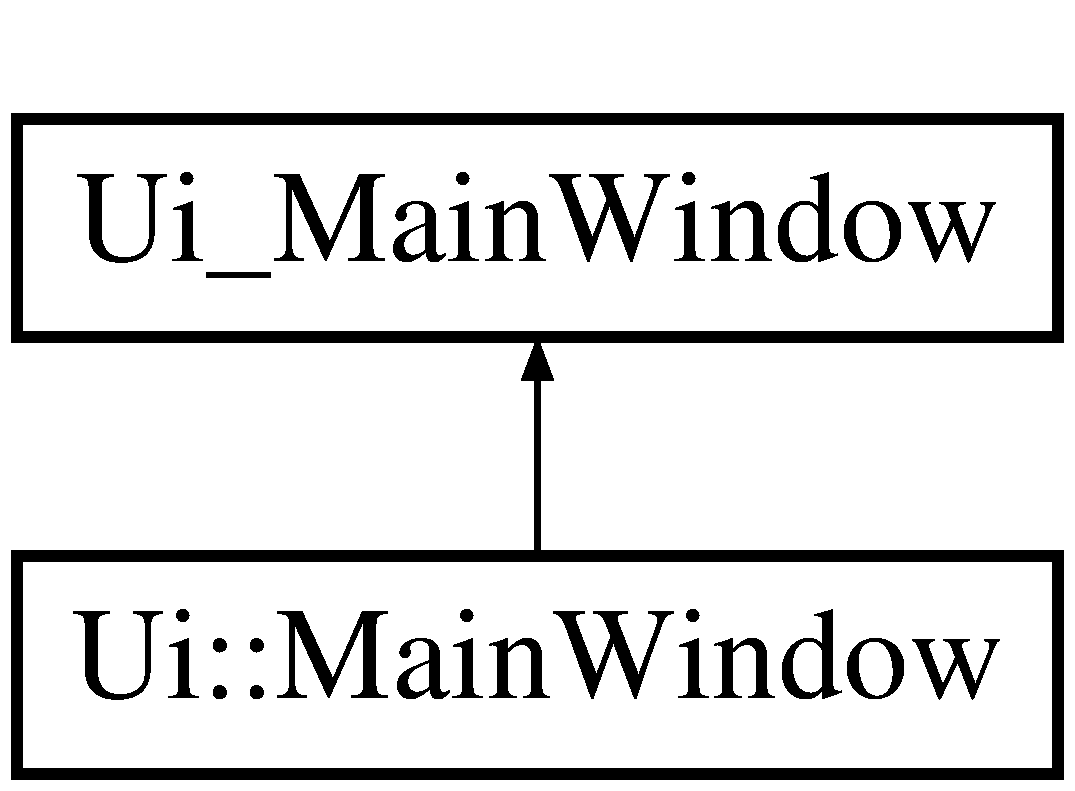
\includegraphics[height=2.000000cm]{df/dd7/class_ui___main_window}
\end{center}
\end{figure}
\subsection*{Public Member Functions}
\begin{DoxyCompactItemize}
\item 
void \textbf{ setup\+Ui} (Q\+Main\+Window $\ast$\textbf{ Main\+Window})
\item 
void \textbf{ retranslate\+Ui} (Q\+Main\+Window $\ast$\textbf{ Main\+Window})
\end{DoxyCompactItemize}
\subsection*{Public Attributes}
\begin{DoxyCompactItemize}
\item 
Q\+Menu\+Bar $\ast$ \textbf{ menu\+Bar}
\item 
Q\+Tool\+Bar $\ast$ \textbf{ main\+Tool\+Bar}
\item 
Q\+Widget $\ast$ \textbf{ central\+Widget}
\item 
Q\+Status\+Bar $\ast$ \textbf{ status\+Bar}
\end{DoxyCompactItemize}


\subsection{Detailed Description}


Definition at line 25 of file ui\+\_\+mainwindow.\+h.



\subsection{Member Function Documentation}
\mbox{\label{class_ui___main_window_a097dd160c3534a204904cb374412c618}} 
\index{Ui\+\_\+\+Main\+Window@{Ui\+\_\+\+Main\+Window}!retranslate\+Ui@{retranslate\+Ui}}
\index{retranslate\+Ui@{retranslate\+Ui}!Ui\+\_\+\+Main\+Window@{Ui\+\_\+\+Main\+Window}}
\subsubsection{retranslate\+Ui()}
{\footnotesize\ttfamily void Ui\+\_\+\+Main\+Window\+::retranslate\+Ui (\begin{DoxyParamCaption}\item[{Q\+Main\+Window $\ast$}]{Main\+Window }\end{DoxyParamCaption})\hspace{0.3cm}{\ttfamily [inline]}}



Definition at line 56 of file ui\+\_\+mainwindow.\+h.

\mbox{\label{class_ui___main_window_acf4a0872c4c77d8f43a2ec66ed849b58}} 
\index{Ui\+\_\+\+Main\+Window@{Ui\+\_\+\+Main\+Window}!setup\+Ui@{setup\+Ui}}
\index{setup\+Ui@{setup\+Ui}!Ui\+\_\+\+Main\+Window@{Ui\+\_\+\+Main\+Window}}
\subsubsection{setup\+Ui()}
{\footnotesize\ttfamily void Ui\+\_\+\+Main\+Window\+::setup\+Ui (\begin{DoxyParamCaption}\item[{Q\+Main\+Window $\ast$}]{Main\+Window }\end{DoxyParamCaption})\hspace{0.3cm}{\ttfamily [inline]}}



Definition at line 33 of file ui\+\_\+mainwindow.\+h.



\subsection{Member Data Documentation}
\mbox{\label{class_ui___main_window_a30075506c2116c3ed4ff25e07ae75f81}} 
\index{Ui\+\_\+\+Main\+Window@{Ui\+\_\+\+Main\+Window}!central\+Widget@{central\+Widget}}
\index{central\+Widget@{central\+Widget}!Ui\+\_\+\+Main\+Window@{Ui\+\_\+\+Main\+Window}}
\subsubsection{central\+Widget}
{\footnotesize\ttfamily Q\+Widget$\ast$ Ui\+\_\+\+Main\+Window\+::central\+Widget}



Definition at line 30 of file ui\+\_\+mainwindow.\+h.

\mbox{\label{class_ui___main_window_a5172877001c8c7b4e0f6de50421867d1}} 
\index{Ui\+\_\+\+Main\+Window@{Ui\+\_\+\+Main\+Window}!main\+Tool\+Bar@{main\+Tool\+Bar}}
\index{main\+Tool\+Bar@{main\+Tool\+Bar}!Ui\+\_\+\+Main\+Window@{Ui\+\_\+\+Main\+Window}}
\subsubsection{main\+Tool\+Bar}
{\footnotesize\ttfamily Q\+Tool\+Bar$\ast$ Ui\+\_\+\+Main\+Window\+::main\+Tool\+Bar}



Definition at line 29 of file ui\+\_\+mainwindow.\+h.

\mbox{\label{class_ui___main_window_a2be1c24ec9adfca18e1dcc951931457f}} 
\index{Ui\+\_\+\+Main\+Window@{Ui\+\_\+\+Main\+Window}!menu\+Bar@{menu\+Bar}}
\index{menu\+Bar@{menu\+Bar}!Ui\+\_\+\+Main\+Window@{Ui\+\_\+\+Main\+Window}}
\subsubsection{menu\+Bar}
{\footnotesize\ttfamily Q\+Menu\+Bar$\ast$ Ui\+\_\+\+Main\+Window\+::menu\+Bar}



Definition at line 28 of file ui\+\_\+mainwindow.\+h.

\mbox{\label{class_ui___main_window_a50fa481337604bcc8bf68de18ab16ecd}} 
\index{Ui\+\_\+\+Main\+Window@{Ui\+\_\+\+Main\+Window}!status\+Bar@{status\+Bar}}
\index{status\+Bar@{status\+Bar}!Ui\+\_\+\+Main\+Window@{Ui\+\_\+\+Main\+Window}}
\subsubsection{status\+Bar}
{\footnotesize\ttfamily Q\+Status\+Bar$\ast$ Ui\+\_\+\+Main\+Window\+::status\+Bar}



Definition at line 31 of file ui\+\_\+mainwindow.\+h.



The documentation for this class was generated from the following file\+:\begin{DoxyCompactItemize}
\item 
src/\+E\+C\+M\+\_\+\+Main\+Window/\textbf{ ui\+\_\+mainwindow.\+h}\end{DoxyCompactItemize}

\section{Valid\+Response Class Reference}
\label{class_valid_response}\index{Valid\+Response@{Valid\+Response}}


{\ttfamily \#include $<$valid\+\_\+response.\+h$>$}

\subsection*{Public Member Functions}
\begin{DoxyCompactItemize}
\item 
\textbf{ Valid\+Response} ()
\end{DoxyCompactItemize}


\subsection{Detailed Description}


Definition at line 5 of file valid\+\_\+response.\+h.



\subsection{Constructor \& Destructor Documentation}
\mbox{\label{class_valid_response_add95811cd0e150f056ee0945d7c9ccc1}} 
\index{Valid\+Response@{Valid\+Response}!Valid\+Response@{Valid\+Response}}
\index{Valid\+Response@{Valid\+Response}!Valid\+Response@{Valid\+Response}}
\subsubsection{Valid\+Response()}
{\footnotesize\ttfamily Valid\+Response\+::\+Valid\+Response (\begin{DoxyParamCaption}{ }\end{DoxyParamCaption})}



Definition at line 3 of file valid\+\_\+response.\+cpp.



The documentation for this class was generated from the following files\+:\begin{DoxyCompactItemize}
\item 
src/library\+\_\+munk\+\_\+power\+\_\+supply/data\+\_\+response/\textbf{ valid\+\_\+response.\+h}\item 
src/library\+\_\+munk\+\_\+power\+\_\+supply/data\+\_\+response/\textbf{ valid\+\_\+response.\+cpp}\end{DoxyCompactItemize}

\chapter{File Documentation}
\section{src/common/common.cpp File Reference}
\label{common_8cpp}\index{src/common/common.\+cpp@{src/common/common.\+cpp}}
{\ttfamily \#include \char`\"{}common.\+h\char`\"{}}\newline

\section{src/common/common.h File Reference}
\label{common_8h}\index{src/common/common.\+h@{src/common/common.\+h}}
{\ttfamily \#include \char`\"{}common\+\_\+global.\+h\char`\"{}}\newline
\subsection*{Classes}
\begin{DoxyCompactItemize}
\item 
class \textbf{ Common}
\end{DoxyCompactItemize}
\subsection*{Macros}
\begin{DoxyCompactItemize}
\item 
\#define \textbf{ U\+N\+U\+S\+ED}(x)~(void)(x)
\end{DoxyCompactItemize}


\subsection{Macro Definition Documentation}
\mbox{\label{common_8h_a86d500a34c624c2cae56bc25a31b12f3}} 
\index{common.\+h@{common.\+h}!U\+N\+U\+S\+ED@{U\+N\+U\+S\+ED}}
\index{U\+N\+U\+S\+ED@{U\+N\+U\+S\+ED}!common.\+h@{common.\+h}}
\subsubsection{U\+N\+U\+S\+ED}
{\footnotesize\ttfamily \#define U\+N\+U\+S\+ED(\begin{DoxyParamCaption}\item[{}]{x }\end{DoxyParamCaption})~(void)(x)}



Definition at line 6 of file common.\+h.


\section{src/common/common\+\_\+global.h File Reference}
\label{common__global_8h}\index{src/common/common\+\_\+global.\+h@{src/common/common\+\_\+global.\+h}}
\subsection*{Macros}
\begin{DoxyCompactItemize}
\item 
\#define \textbf{ C\+O\+M\+M\+O\+N\+S\+H\+A\+R\+E\+D\+\_\+\+E\+X\+P\+O\+RT}
\end{DoxyCompactItemize}


\subsection{Macro Definition Documentation}
\mbox{\label{common__global_8h_a84fbd581e036ee185e23f61bcf89a44e}} 
\index{common\+\_\+global.\+h@{common\+\_\+global.\+h}!C\+O\+M\+M\+O\+N\+S\+H\+A\+R\+E\+D\+\_\+\+E\+X\+P\+O\+RT@{C\+O\+M\+M\+O\+N\+S\+H\+A\+R\+E\+D\+\_\+\+E\+X\+P\+O\+RT}}
\index{C\+O\+M\+M\+O\+N\+S\+H\+A\+R\+E\+D\+\_\+\+E\+X\+P\+O\+RT@{C\+O\+M\+M\+O\+N\+S\+H\+A\+R\+E\+D\+\_\+\+E\+X\+P\+O\+RT}!common\+\_\+global.\+h@{common\+\_\+global.\+h}}
\subsubsection{C\+O\+M\+M\+O\+N\+S\+H\+A\+R\+E\+D\+\_\+\+E\+X\+P\+O\+RT}
{\footnotesize\ttfamily \#define C\+O\+M\+M\+O\+N\+S\+H\+A\+R\+E\+D\+\_\+\+E\+X\+P\+O\+RT}



Definition at line 11 of file common\+\_\+global.\+h.


\section{src/\+E\+C\+M\+\_\+\+Main\+Window/main.cpp File Reference}
\label{_e_c_m___main_window_2main_8cpp}\index{src/\+E\+C\+M\+\_\+\+Main\+Window/main.\+cpp@{src/\+E\+C\+M\+\_\+\+Main\+Window/main.\+cpp}}
{\ttfamily \#include \char`\"{}mainwindow.\+h\char`\"{}}\newline
{\ttfamily \#include $<$Q\+Application$>$}\newline
\subsection*{Functions}
\begin{DoxyCompactItemize}
\item 
int \textbf{ main} (int argc, char $\ast$argv[$\,$])
\end{DoxyCompactItemize}


\subsection{Function Documentation}
\mbox{\label{_e_c_m___main_window_2main_8cpp_a0ddf1224851353fc92bfbff6f499fa97}} 
\index{E\+C\+M\+\_\+\+Main\+Window/main.\+cpp@{E\+C\+M\+\_\+\+Main\+Window/main.\+cpp}!main@{main}}
\index{main@{main}!E\+C\+M\+\_\+\+Main\+Window/main.\+cpp@{E\+C\+M\+\_\+\+Main\+Window/main.\+cpp}}
\subsubsection{main()}
{\footnotesize\ttfamily int main (\begin{DoxyParamCaption}\item[{int}]{argc,  }\item[{char $\ast$}]{argv[$\,$] }\end{DoxyParamCaption})}



Definition at line 4 of file main.\+cpp.


\section{src/\+Window\+\_\+\+Munk\+Power\+Supply/main.cpp File Reference}
\label{_window___munk_power_supply_2main_8cpp}\index{src/\+Window\+\_\+\+Munk\+Power\+Supply/main.\+cpp@{src/\+Window\+\_\+\+Munk\+Power\+Supply/main.\+cpp}}
{\ttfamily \#include \char`\"{}mainwindow.\+h\char`\"{}}\newline
{\ttfamily \#include $<$Q\+Application$>$}\newline
\subsection*{Functions}
\begin{DoxyCompactItemize}
\item 
int \textbf{ main} (int argc, char $\ast$argv[$\,$])
\end{DoxyCompactItemize}


\subsection{Function Documentation}
\mbox{\label{_window___munk_power_supply_2main_8cpp_a0ddf1224851353fc92bfbff6f499fa97}} 
\index{Window\+\_\+\+Munk\+Power\+Supply/main.\+cpp@{Window\+\_\+\+Munk\+Power\+Supply/main.\+cpp}!main@{main}}
\index{main@{main}!Window\+\_\+\+Munk\+Power\+Supply/main.\+cpp@{Window\+\_\+\+Munk\+Power\+Supply/main.\+cpp}}
\subsubsection{main()}
{\footnotesize\ttfamily int main (\begin{DoxyParamCaption}\item[{int}]{argc,  }\item[{char $\ast$}]{argv[$\,$] }\end{DoxyParamCaption})}



Definition at line 4 of file main.\+cpp.


\section{src/\+E\+C\+M\+\_\+\+Main\+Window/mainwindow.cpp File Reference}
\label{_e_c_m___main_window_2mainwindow_8cpp}\index{src/\+E\+C\+M\+\_\+\+Main\+Window/mainwindow.\+cpp@{src/\+E\+C\+M\+\_\+\+Main\+Window/mainwindow.\+cpp}}
{\ttfamily \#include \char`\"{}mainwindow.\+h\char`\"{}}\newline
{\ttfamily \#include \char`\"{}ui\+\_\+mainwindow.\+h\char`\"{}}\newline

\section{src/\+Window\+\_\+\+Munk\+Power\+Supply/mainwindow.cpp File Reference}
\label{_window___munk_power_supply_2mainwindow_8cpp}\index{src/\+Window\+\_\+\+Munk\+Power\+Supply/mainwindow.\+cpp@{src/\+Window\+\_\+\+Munk\+Power\+Supply/mainwindow.\+cpp}}
{\ttfamily \#include \char`\"{}mainwindow.\+h\char`\"{}}\newline
{\ttfamily \#include \char`\"{}ui\+\_\+mainwindow.\+h\char`\"{}}\newline
{\ttfamily \#include \char`\"{}library\+\_\+munk\+\_\+power\+\_\+supply/data/type\+\_\+segment\+\_\+level.\+h\char`\"{}}\newline
{\ttfamily \#include \char`\"{}library\+\_\+munk\+\_\+power\+\_\+supply/data/type\+\_\+segment\+\_\+mode.\+h\char`\"{}}\newline
{\ttfamily \#include \char`\"{}library\+\_\+munk\+\_\+power\+\_\+supply/data/type\+\_\+read\+\_\+write.\+h\char`\"{}}\newline
{\ttfamily \#include \char`\"{}library\+\_\+munk\+\_\+power\+\_\+supply/data/type\+\_\+prescalar\+\_\+power.\+h\char`\"{}}\newline
{\ttfamily \#include \char`\"{}library\+\_\+munk\+\_\+power\+\_\+supply/data\+\_\+registers/segment\+\_\+time\+\_\+general.\+h\char`\"{}}\newline
{\ttfamily \#include \char`\"{}data\+\_\+registers/segment\+\_\+time\+\_\+detailed.\+h\char`\"{}}\newline

\section{src/\+E\+C\+M\+\_\+\+Main\+Window/mainwindow.h File Reference}
\label{_e_c_m___main_window_2mainwindow_8h}\index{src/\+E\+C\+M\+\_\+\+Main\+Window/mainwindow.\+h@{src/\+E\+C\+M\+\_\+\+Main\+Window/mainwindow.\+h}}
{\ttfamily \#include $<$Q\+Byte\+Array$>$}\newline
{\ttfamily \#include $<$Q\+String$>$}\newline
{\ttfamily \#include $<$Qt\+Debug$>$}\newline
{\ttfamily \#include $<$iostream$>$}\newline
{\ttfamily \#include $<$Q\+Main\+Window$>$}\newline
{\ttfamily \#include $<$vector$>$}\newline
{\ttfamily \#include $<$limits.\+h$>$}\newline
{\ttfamily \#include \char`\"{}library\+\_\+munk\+\_\+power\+\_\+supply/munk\+\_\+power\+\_\+supply.\+h\char`\"{}}\newline
{\ttfamily \#include \char`\"{}library\+\_\+munk\+\_\+power\+\_\+supply/data\+\_\+registers/segment\+\_\+time\+\_\+general.\+h\char`\"{}}\newline
\subsection*{Classes}
\begin{DoxyCompactItemize}
\item 
class \textbf{ Main\+Window}
\end{DoxyCompactItemize}
\subsection*{Namespaces}
\begin{DoxyCompactItemize}
\item 
 \textbf{ Ui}
\end{DoxyCompactItemize}

\section{src/\+Window\+\_\+\+Munk\+Power\+Supply/mainwindow.h File Reference}
\label{_window___munk_power_supply_2mainwindow_8h}\index{src/\+Window\+\_\+\+Munk\+Power\+Supply/mainwindow.\+h@{src/\+Window\+\_\+\+Munk\+Power\+Supply/mainwindow.\+h}}
{\ttfamily \#include $<$iostream$>$}\newline
{\ttfamily \#include $<$Q\+Debug$>$}\newline
{\ttfamily \#include \char`\"{}library\+\_\+munk\+\_\+power\+\_\+supply\+\_\+global.\+h\char`\"{}}\newline
{\ttfamily \#include $<$Q\+Main\+Window$>$}\newline
{\ttfamily \#include $<$Q\+Byte\+Array$>$}\newline
\subsection*{Classes}
\begin{DoxyCompactItemize}
\item 
class \textbf{ Main\+Window}
\end{DoxyCompactItemize}
\subsection*{Namespaces}
\begin{DoxyCompactItemize}
\item 
 \textbf{ Ui}
\end{DoxyCompactItemize}

\section{src/\+E\+C\+M\+\_\+\+Main\+Window/ui\+\_\+mainwindow.h File Reference}
\label{ui__mainwindow_8h}\index{src/\+E\+C\+M\+\_\+\+Main\+Window/ui\+\_\+mainwindow.\+h@{src/\+E\+C\+M\+\_\+\+Main\+Window/ui\+\_\+mainwindow.\+h}}
{\ttfamily \#include $<$Qt\+Core/\+Q\+Variant$>$}\newline
{\ttfamily \#include $<$Qt\+Widgets/\+Q\+Action$>$}\newline
{\ttfamily \#include $<$Qt\+Widgets/\+Q\+Application$>$}\newline
{\ttfamily \#include $<$Qt\+Widgets/\+Q\+Button\+Group$>$}\newline
{\ttfamily \#include $<$Qt\+Widgets/\+Q\+Header\+View$>$}\newline
{\ttfamily \#include $<$Qt\+Widgets/\+Q\+Main\+Window$>$}\newline
{\ttfamily \#include $<$Qt\+Widgets/\+Q\+Menu\+Bar$>$}\newline
{\ttfamily \#include $<$Qt\+Widgets/\+Q\+Status\+Bar$>$}\newline
{\ttfamily \#include $<$Qt\+Widgets/\+Q\+Tool\+Bar$>$}\newline
{\ttfamily \#include $<$Qt\+Widgets/\+Q\+Widget$>$}\newline
\subsection*{Classes}
\begin{DoxyCompactItemize}
\item 
class \textbf{ Ui\+\_\+\+Main\+Window}
\item 
class \textbf{ Ui\+::\+Main\+Window}
\end{DoxyCompactItemize}
\subsection*{Namespaces}
\begin{DoxyCompactItemize}
\item 
 \textbf{ Ui}
\end{DoxyCompactItemize}

\section{src/library\+\_\+munk\+\_\+power\+\_\+supply/data/fault\+\_\+codes\+\_\+register\+\_\+one.h File Reference}
\label{fault__codes__register__one_8h}\index{src/library\+\_\+munk\+\_\+power\+\_\+supply/data/fault\+\_\+codes\+\_\+register\+\_\+one.\+h@{src/library\+\_\+munk\+\_\+power\+\_\+supply/data/fault\+\_\+codes\+\_\+register\+\_\+one.\+h}}
{\ttfamily \#include $<$string$>$}\newline
{\ttfamily \#include $<$stdexcept$>$}\newline
{\ttfamily \#include $<$vector$>$}\newline
\subsection*{Namespaces}
\begin{DoxyCompactItemize}
\item 
 \textbf{ Data}
\end{DoxyCompactItemize}
\subsection*{Enumerations}
\begin{DoxyCompactItemize}
\item 
enum \textbf{ Data\+::\+Fault\+Codes\+Register1} \{ \newline
\textbf{ Data\+::\+Fault\+Codes\+Register1\+::\+E\+R\+R\+\_\+\+F\+R1\+\_\+\+D\+C\+L\+I\+N\+K\+\_\+\+O\+FF} = 1, 
\textbf{ Data\+::\+Fault\+Codes\+Register1\+::\+E\+R\+R\+\_\+\+F\+R1\+\_\+\+D\+S\+P\+\_\+\+P\+W\+M1\+\_\+\+G\+E\+N\+E\+R\+A\+T\+OR} = 2, 
\textbf{ Data\+::\+Fault\+Codes\+Register1\+::\+E\+R\+R\+\_\+\+F\+R1\+\_\+\+D\+S\+P\+\_\+\+P\+W\+M2\+\_\+\+G\+E\+N\+E\+R\+A\+T\+OR} = 4, 
\textbf{ Data\+::\+Fault\+Codes\+Register1\+::\+E\+R\+R\+\_\+\+F\+R1\+\_\+\+D\+S\+P\+\_\+\+E\+R\+R\+OR} = 8, 
\newline
\textbf{ Data\+::\+Fault\+Codes\+Register1\+::\+E\+R\+R\+\_\+\+F\+R1\+\_\+\+D\+S\+P\+\_\+\+P\+I\+C\+\_\+\+D\+E\+AD} = 16, 
\textbf{ Data\+::\+Fault\+Codes\+Register1\+::\+E\+R\+R\+\_\+\+F\+R1\+\_\+\+D\+S\+P\+\_\+\+T\+I\+C\+K\+C\+O\+U\+N\+T\+\_\+\+E\+R\+R\+OR} = 32, 
\textbf{ Data\+::\+Fault\+Codes\+Register1\+::\+E\+R\+R\+\_\+\+F\+R1\+\_\+\+I\+N\+T\+E\+R\+N\+A\+L\+\_\+\+E\+R\+R\+OR} = 64, 
\textbf{ Data\+::\+Fault\+Codes\+Register1\+::\+E\+R\+R\+\_\+\+F\+R1\+\_\+\+E\+X\+T\+C\+O\+M\+M2} = 128, 
\newline
\textbf{ Data\+::\+Fault\+Codes\+Register1\+::\+E\+R\+R\+\_\+\+F\+R1\+\_\+\+C\+H\+A\+R\+G\+I\+NG} = 256, 
\textbf{ Data\+::\+Fault\+Codes\+Register1\+::\+E\+R\+R\+\_\+\+F\+R1\+\_\+\+T\+E\+M\+P\+\_\+\+P\+O\+W\+E\+R\+B\+O\+A\+RD} = 512, 
\textbf{ Data\+::\+Fault\+Codes\+Register1\+::\+E\+R\+R\+\_\+\+F\+R1\+\_\+\+E\+X\+T\+C\+O\+M\+M1} = 1024, 
\textbf{ Data\+::\+Fault\+Codes\+Register1\+::\+E\+R\+R\+\_\+\+F\+R1\+\_\+\+S\+Y\+N\+C\+H\+RO} = 2048, 
\newline
\textbf{ Data\+::\+Fault\+Codes\+Register1\+::\+E\+R\+R\+\_\+\+F\+R1\+\_\+\+T\+E\+M\+P\+\_\+\+M\+A\+I\+N\+S\+C\+O\+N\+T\+R\+O\+L\+L\+ER} = 4096, 
\textbf{ Data\+::\+Fault\+Codes\+Register1\+::\+E\+R\+R\+\_\+\+F\+R1\+\_\+\+Z\+E\+R\+O\+B\+A\+T\+CH} = 8192, 
\textbf{ Data\+::\+Fault\+Codes\+Register1\+::\+E\+R\+R\+\_\+\+F\+R1\+\_\+\+G\+E\+N\+E\+R\+A\+L\+\_\+\+O\+V\+E\+R\+C\+U\+R\+R\+E\+NT} = 16384, 
\textbf{ Data\+::\+Fault\+Codes\+Register1\+::\+E\+R\+R\+\_\+\+F\+R1\+\_\+\+G\+E\+N\+E\+R\+A\+L\+\_\+\+O\+V\+E\+R\+V\+O\+L\+T\+A\+GE} = 32768
 \}\begin{DoxyCompactList}\small\item\em The Current\+Factor\+Type enum. \end{DoxyCompactList}
\end{DoxyCompactItemize}

\section{src/library\+\_\+munk\+\_\+power\+\_\+supply/data/fault\+\_\+codes\+\_\+register\+\_\+three.h File Reference}
\label{fault__codes__register__three_8h}\index{src/library\+\_\+munk\+\_\+power\+\_\+supply/data/fault\+\_\+codes\+\_\+register\+\_\+three.\+h@{src/library\+\_\+munk\+\_\+power\+\_\+supply/data/fault\+\_\+codes\+\_\+register\+\_\+three.\+h}}
{\ttfamily \#include $<$string$>$}\newline
{\ttfamily \#include $<$stdexcept$>$}\newline
{\ttfamily \#include $<$vector$>$}\newline
\subsection*{Namespaces}
\begin{DoxyCompactItemize}
\item 
 \textbf{ Data}
\end{DoxyCompactItemize}
\subsection*{Enumerations}
\begin{DoxyCompactItemize}
\item 
enum \textbf{ Data\+::\+Fault\+Codes\+Register3} \{ \newline
\textbf{ Data\+::\+Fault\+Codes\+Register3\+::\+E\+R\+R\+\_\+\+F\+R3\+\_\+\+E\+X\+T\+E\+R\+N\+A\+L\+\_\+\+T\+R\+I\+P1} = 1, 
\textbf{ Data\+::\+Fault\+Codes\+Register3\+::\+E\+R\+R\+\_\+\+F\+R3\+\_\+\+E\+X\+T\+E\+R\+N\+A\+L\+\_\+\+T\+R\+I\+P2} = 2, 
\textbf{ Data\+::\+Fault\+Codes\+Register3\+::\+E\+R\+R\+\_\+\+F\+R3\+\_\+\+P\+L\+D\+\_\+\+P\+W\+M\+\_\+\+G\+E\+N\+E\+R\+A\+T\+O\+R1} = 4, 
\textbf{ Data\+::\+Fault\+Codes\+Register3\+::\+E\+R\+R\+\_\+\+F\+R3\+\_\+\+P\+L\+D\+\_\+\+P\+W\+M\+\_\+\+G\+E\+N\+E\+R\+A\+T\+O\+R2} = 8, 
\newline
\textbf{ Data\+::\+Fault\+Codes\+Register3\+::\+E\+R\+R\+\_\+\+F\+R3\+\_\+\+L\+O\+S\+T\+\_\+\+F\+I\+E\+L\+D\+B\+US} = 16, 
\textbf{ Data\+::\+Fault\+Codes\+Register3\+::\+E\+R\+R\+\_\+\+F\+R3\+\_\+\+D\+Y\+N\+A\+M\+I\+C\+\_\+\+O\+V\+E\+R\+C\+U\+R\+R\+E\+NT} = 32, 
\textbf{ Data\+::\+Fault\+Codes\+Register3\+::\+E\+R\+R\+\_\+\+F\+R3\+\_\+\+R\+E\+S\+E\+R\+V\+E\+D\+\_\+7} = 64, 
\textbf{ Data\+::\+Fault\+Codes\+Register3\+::\+E\+R\+R\+\_\+\+F\+R3\+\_\+\+R\+E\+S\+E\+R\+V\+E\+D\+\_\+8} = 128, 
\newline
\textbf{ Data\+::\+Fault\+Codes\+Register3\+::\+E\+R\+R\+\_\+\+F\+R3\+\_\+\+R\+E\+S\+E\+R\+V\+E\+D\+\_\+9} = 256, 
\textbf{ Data\+::\+Fault\+Codes\+Register3\+::\+E\+R\+R\+\_\+\+F\+R3\+\_\+\+R\+E\+S\+E\+R\+V\+E\+D\+\_\+10} = 512, 
\textbf{ Data\+::\+Fault\+Codes\+Register3\+::\+E\+R\+R\+\_\+\+F\+R3\+\_\+\+R\+E\+S\+E\+R\+V\+E\+D\+\_\+11} = 1024, 
\textbf{ Data\+::\+Fault\+Codes\+Register3\+::\+E\+R\+R\+\_\+\+F\+R3\+\_\+\+R\+E\+S\+E\+R\+V\+E\+D\+\_\+12} = 2048, 
\newline
\textbf{ Data\+::\+Fault\+Codes\+Register3\+::\+E\+R\+R\+\_\+\+F\+R3\+\_\+\+R\+E\+S\+E\+R\+V\+E\+D\+\_\+13} = 4096, 
\textbf{ Data\+::\+Fault\+Codes\+Register3\+::\+E\+R\+R\+\_\+\+F\+R3\+\_\+\+R\+E\+S\+E\+R\+V\+E\+D\+\_\+14} = 8192, 
\textbf{ Data\+::\+Fault\+Codes\+Register3\+::\+E\+R\+R\+\_\+\+F\+R3\+\_\+\+R\+E\+S\+E\+R\+V\+E\+D\+\_\+15} = 16384, 
\textbf{ Data\+::\+Fault\+Codes\+Register3\+::\+E\+R\+R\+\_\+\+F\+R3\+\_\+\+R\+E\+S\+E\+R\+V\+E\+D\+\_\+16} = 32768
 \}\begin{DoxyCompactList}\small\item\em The Current\+Factor\+Type enum. \end{DoxyCompactList}
\end{DoxyCompactItemize}

\section{src/library\+\_\+munk\+\_\+power\+\_\+supply/data/fault\+\_\+codes\+\_\+register\+\_\+two.h File Reference}
\label{fault__codes__register__two_8h}\index{src/library\+\_\+munk\+\_\+power\+\_\+supply/data/fault\+\_\+codes\+\_\+register\+\_\+two.\+h@{src/library\+\_\+munk\+\_\+power\+\_\+supply/data/fault\+\_\+codes\+\_\+register\+\_\+two.\+h}}
{\ttfamily \#include $<$string$>$}\newline
{\ttfamily \#include $<$stdexcept$>$}\newline
{\ttfamily \#include $<$vector$>$}\newline
\subsection*{Namespaces}
\begin{DoxyCompactItemize}
\item 
 \textbf{ Data}
\end{DoxyCompactItemize}
\subsection*{Enumerations}
\begin{DoxyCompactItemize}
\item 
enum \textbf{ Data\+::\+Fault\+Codes\+Register2} \{ \newline
\textbf{ Data\+::\+Fault\+Codes\+Register2\+::\+E\+R\+R\+\_\+\+F\+R2\+\_\+\+A\+M\+P\+H\+O\+U\+R\+C\+H\+E\+C\+K\+S\+UM} = 1, 
\textbf{ Data\+::\+Fault\+Codes\+Register2\+::\+E\+R\+R\+\_\+\+F\+R2\+\_\+\+I\+N\+T\+\_\+\+E\+E\+P\+R\+OM} = 2, 
\textbf{ Data\+::\+Fault\+Codes\+Register2\+::\+E\+R\+R\+\_\+\+F\+R2\+\_\+\+E\+X\+T\+\_\+\+E\+E\+P\+R\+OM} = 4, 
\textbf{ Data\+::\+Fault\+Codes\+Register2\+::\+E\+R\+R\+\_\+\+F\+R2\+\_\+\+E\+E\+P\+R\+O\+M\+\_\+\+F\+O\+R\+M\+AT} = 8, 
\newline
\textbf{ Data\+::\+Fault\+Codes\+Register2\+::\+E\+R\+R\+\_\+\+F\+R2\+\_\+\+B\+A\+T\+C\+H\+\_\+\+R\+E\+AD} = 16, 
\textbf{ Data\+::\+Fault\+Codes\+Register2\+::\+E\+R\+R\+\_\+\+F\+R2\+\_\+\+B\+A\+T\+C\+H\+\_\+\+W\+R\+I\+TE} = 32, 
\textbf{ Data\+::\+Fault\+Codes\+Register2\+::\+E\+R\+R\+\_\+\+F\+R2\+\_\+\+P\+A\+T\+T\+E\+R\+N\+\_\+\+R\+E\+AD} = 64, 
\textbf{ Data\+::\+Fault\+Codes\+Register2\+::\+E\+R\+R\+\_\+\+F\+R2\+\_\+\+P\+A\+T\+T\+E\+R\+N\+\_\+\+W\+R\+I\+TE} = 128, 
\newline
\textbf{ Data\+::\+Fault\+Codes\+Register2\+::\+E\+R\+R\+\_\+\+F\+R2\+\_\+\+I\+D\+C\+L\+I\+N\+K\+\_\+\+I\+X\+T\+\_\+\+T\+R\+I\+P1} = 256, 
\textbf{ Data\+::\+Fault\+Codes\+Register2\+::\+E\+R\+R\+\_\+\+F\+R2\+\_\+\+C\+O\+N\+T\+R\+O\+L\+S\+U\+P\+P\+LY} = 512, 
\textbf{ Data\+::\+Fault\+Codes\+Register2\+::\+E\+R\+R\+\_\+\+F\+R2\+\_\+\+D\+C\+L\+I\+N\+K1} = 1024, 
\textbf{ Data\+::\+Fault\+Codes\+Register2\+::\+E\+R\+R\+\_\+\+F\+R2\+\_\+\+P\+L\+D\+\_\+1\+\_\+5\+\_\+\+S\+U\+P\+P\+LY} = 2048, 
\newline
\textbf{ Data\+::\+Fault\+Codes\+Register2\+::\+E\+R\+R\+\_\+\+F\+R2\+\_\+\+I\+D\+C\+L\+I\+N\+K\+\_\+\+I\+X\+T\+\_\+\+T\+R\+I\+P2} = 4096, 
\textbf{ Data\+::\+Fault\+Codes\+Register2\+::\+E\+R\+R\+\_\+\+F\+R2\+\_\+\+D\+C\+L\+I\+N\+K2} = 8192, 
\textbf{ Data\+::\+Fault\+Codes\+Register2\+::\+E\+R\+R\+\_\+\+F\+R2\+\_\+\+R\+E\+S\+E\+R\+V\+ED} = 16384, 
\textbf{ Data\+::\+Fault\+Codes\+Register2\+::\+E\+R\+R\+\_\+\+F\+R2\+\_\+\+S\+E\+T\+\_\+\+C\+U\+R\+R\+E\+N\+T\+\_\+\+E\+X\+C\+E\+E\+D\+ED} = 32768
 \}\begin{DoxyCompactList}\small\item\em The Current\+Factor\+Type enum. \end{DoxyCompactList}
\end{DoxyCompactItemize}

\section{src/library\+\_\+munk\+\_\+power\+\_\+supply/data/register\+\_\+data\+\_\+object.cpp File Reference}
\label{register__data__object_8cpp}\index{src/library\+\_\+munk\+\_\+power\+\_\+supply/data/register\+\_\+data\+\_\+object.\+cpp@{src/library\+\_\+munk\+\_\+power\+\_\+supply/data/register\+\_\+data\+\_\+object.\+cpp}}
{\ttfamily \#include \char`\"{}register\+\_\+data\+\_\+object.\+h\char`\"{}}\newline
\subsection*{Namespaces}
\begin{DoxyCompactItemize}
\item 
 \textbf{ Data}
\end{DoxyCompactItemize}

\section{src/library\+\_\+munk\+\_\+power\+\_\+supply/data/register\+\_\+data\+\_\+object.h File Reference}
\label{register__data__object_8h}\index{src/library\+\_\+munk\+\_\+power\+\_\+supply/data/register\+\_\+data\+\_\+object.\+h@{src/library\+\_\+munk\+\_\+power\+\_\+supply/data/register\+\_\+data\+\_\+object.\+h}}
{\ttfamily \#include $<$stdint.\+h$>$}\newline
{\ttfamily \#include $<$string$>$}\newline
{\ttfamily \#include $<$stdexcept$>$}\newline
{\ttfamily \#include $<$vector$>$}\newline
\subsection*{Classes}
\begin{DoxyCompactItemize}
\item 
class \textbf{ Data\+::\+Register\+Data\+Object}
\begin{DoxyCompactList}\small\item\em The \doxyref{Register\+Data\+Object}{p.}{df/d53/class_data_1_1_register_data_object} class. \end{DoxyCompactList}\end{DoxyCompactItemize}
\subsection*{Namespaces}
\begin{DoxyCompactItemize}
\item 
 \textbf{ Data}
\end{DoxyCompactItemize}

\section{src/library\+\_\+munk\+\_\+power\+\_\+supply/data/type\+\_\+current\+\_\+factor.h File Reference}
\label{type__current__factor_8h}\index{src/library\+\_\+munk\+\_\+power\+\_\+supply/data/type\+\_\+current\+\_\+factor.\+h@{src/library\+\_\+munk\+\_\+power\+\_\+supply/data/type\+\_\+current\+\_\+factor.\+h}}
{\ttfamily \#include $<$string$>$}\newline
{\ttfamily \#include $<$stdexcept$>$}\newline
{\ttfamily \#include $<$vector$>$}\newline
\subsection*{Namespaces}
\begin{DoxyCompactItemize}
\item 
 \textbf{ Data}
\end{DoxyCompactItemize}
\subsection*{Enumerations}
\begin{DoxyCompactItemize}
\item 
enum \textbf{ Data\+::\+Current\+Factor\+Type} \{ \textbf{ Data\+::\+Current\+Factor\+Type\+::\+A\+M\+PS} = 0, 
\textbf{ Data\+::\+Current\+Factor\+Type\+::\+A\+\_\+\+D\+M2} = 1
 \}\begin{DoxyCompactList}\small\item\em The Current\+Factor\+Type enum. \end{DoxyCompactList}
\end{DoxyCompactItemize}
\subsection*{Functions}
\begin{DoxyCompactItemize}
\item 
std\+::string \textbf{ Data\+::\+Current\+Factor\+To\+String} (const Current\+Factor\+Type \&type)
\begin{DoxyCompactList}\small\item\em Current\+Factor\+To\+String. \end{DoxyCompactList}\item 
Current\+Factor\+Type \textbf{ Data\+::\+Current\+Factor\+From\+String} (const std\+::string \&str)
\begin{DoxyCompactList}\small\item\em Current\+Factor\+From\+String. \end{DoxyCompactList}\item 
std\+::vector$<$ std\+::string $>$ \textbf{ Data\+::get\+List\+Of\+Current\+Factor} ()
\begin{DoxyCompactList}\small\item\em get\+List\+Of\+Current\+Factor \end{DoxyCompactList}\end{DoxyCompactItemize}

\section{src/library\+\_\+munk\+\_\+power\+\_\+supply/data/type\+\_\+current\+\_\+set.h File Reference}
\label{type__current__set_8h}\index{src/library\+\_\+munk\+\_\+power\+\_\+supply/data/type\+\_\+current\+\_\+set.\+h@{src/library\+\_\+munk\+\_\+power\+\_\+supply/data/type\+\_\+current\+\_\+set.\+h}}
{\ttfamily \#include $<$string$>$}\newline
{\ttfamily \#include $<$stdexcept$>$}\newline
{\ttfamily \#include $<$vector$>$}\newline
\subsection*{Namespaces}
\begin{DoxyCompactItemize}
\item 
 \textbf{ Data}
\end{DoxyCompactItemize}
\subsection*{Enumerations}
\begin{DoxyCompactItemize}
\item 
enum \textbf{ Data\+::\+Current\+Set\+F\+W\+D\+Type} \{ \newline
\textbf{ Data\+::\+Current\+Set\+F\+W\+D\+Type\+::\+Current\+F\+W\+D1} = 6000, 
\textbf{ Data\+::\+Current\+Set\+F\+W\+D\+Type\+::\+Current\+F\+W\+D2} = 6040, 
\textbf{ Data\+::\+Current\+Set\+F\+W\+D\+Type\+::\+Current\+F\+W\+D3} = 6080, 
\textbf{ Data\+::\+Current\+Set\+F\+W\+D\+Type\+::\+Current\+F\+W\+D4} = 6120, 
\newline
\textbf{ Data\+::\+Current\+Set\+F\+W\+D\+Type\+::\+Current\+F\+W\+D5} = 6160, 
\textbf{ Data\+::\+Current\+Set\+F\+W\+D\+Type\+::\+Current\+F\+W\+D6} = 6200, 
\textbf{ Data\+::\+Current\+Set\+F\+W\+D\+Type\+::\+Current\+F\+W\+D7} = 6240, 
\textbf{ Data\+::\+Current\+Set\+F\+W\+D\+Type\+::\+Current\+F\+W\+D8} = 6280
 \}\begin{DoxyCompactList}\small\item\em The Current\+Set\+F\+W\+D\+Type enum. \end{DoxyCompactList}
\item 
enum \textbf{ Data\+::\+Current\+Set\+R\+E\+V\+Type} \{ \newline
\textbf{ Data\+::\+Current\+Set\+R\+E\+V\+Type\+::\+Current\+R\+E\+V1} = 6020, 
\textbf{ Data\+::\+Current\+Set\+R\+E\+V\+Type\+::\+Current\+R\+E\+V2} = 6060, 
\textbf{ Data\+::\+Current\+Set\+R\+E\+V\+Type\+::\+Current\+R\+E\+V3} = 6100, 
\textbf{ Data\+::\+Current\+Set\+R\+E\+V\+Type\+::\+Current\+R\+E\+V4} = 6140, 
\newline
\textbf{ Data\+::\+Current\+Set\+R\+E\+V\+Type\+::\+Current\+R\+E\+V5} = 6180, 
\textbf{ Data\+::\+Current\+Set\+R\+E\+V\+Type\+::\+Current\+R\+E\+V6} = 6220, 
\textbf{ Data\+::\+Current\+Set\+R\+E\+V\+Type\+::\+Current\+R\+E\+V7} = 6260, 
\textbf{ Data\+::\+Current\+Set\+R\+E\+V\+Type\+::\+Current\+R\+E\+V8} = 6300
 \}\begin{DoxyCompactList}\small\item\em The Current\+Set\+R\+E\+V\+Type enum. \end{DoxyCompactList}
\end{DoxyCompactItemize}
\subsection*{Functions}
\begin{DoxyCompactItemize}
\item 
std\+::string \textbf{ Data\+::\+Current\+Set\+F\+W\+D\+Type\+To\+String} (const Current\+Set\+F\+W\+D\+Type \&type)
\begin{DoxyCompactList}\small\item\em Current\+Set\+F\+W\+D\+Type\+To\+String. \end{DoxyCompactList}\item 
Current\+Set\+F\+W\+D\+Type \textbf{ Data\+::\+Current\+Set\+F\+W\+D\+Type\+From\+String} (const std\+::string \&str)
\begin{DoxyCompactList}\small\item\em Current\+Set\+F\+W\+D\+Type\+From\+String. \end{DoxyCompactList}\item 
std\+::vector$<$ Current\+Set\+F\+W\+D\+Type $>$ \textbf{ Data\+::get\+List\+Of\+Current\+Set\+F\+W\+D\+Types} ()
\begin{DoxyCompactList}\small\item\em get\+List\+Of\+Current\+Set\+F\+W\+D\+Types \end{DoxyCompactList}\item 
\textbf{ Data\+::\+Current\+Set\+F\+W\+D\+Type} \textbf{ Data\+::get\+R\+E\+V\+Current\+Index} (const int \&index)
\begin{DoxyCompactList}\small\item\em get\+R\+E\+V\+Current\+Index \end{DoxyCompactList}\item 
std\+::string \textbf{ Data\+::\+Current\+Set\+R\+E\+V\+Type\+To\+String} (const Current\+Set\+R\+E\+V\+Type \&type)
\begin{DoxyCompactList}\small\item\em Current\+Set\+R\+E\+V\+Type\+To\+String. \end{DoxyCompactList}\item 
Current\+Set\+R\+E\+V\+Type \textbf{ Data\+::\+Current\+Set\+R\+E\+V\+Type\+From\+String} (const std\+::string \&str)
\begin{DoxyCompactList}\small\item\em Current\+Set\+R\+E\+V\+Type\+From\+String. \end{DoxyCompactList}\item 
std\+::vector$<$ Current\+Set\+R\+E\+V\+Type $>$ \textbf{ Data\+::get\+List\+Of\+Current\+Set\+R\+E\+V\+Types} ()
\begin{DoxyCompactList}\small\item\em get\+List\+Of\+Current\+Set\+R\+E\+V\+Types \end{DoxyCompactList}\end{DoxyCompactItemize}

\section{src/library\+\_\+munk\+\_\+power\+\_\+supply/data/type\+\_\+current\+\_\+voltage\+\_\+prescale.h File Reference}
\label{type__current__voltage__prescale_8h}\index{src/library\+\_\+munk\+\_\+power\+\_\+supply/data/type\+\_\+current\+\_\+voltage\+\_\+prescale.\+h@{src/library\+\_\+munk\+\_\+power\+\_\+supply/data/type\+\_\+current\+\_\+voltage\+\_\+prescale.\+h}}
{\ttfamily \#include $<$string$>$}\newline
{\ttfamily \#include $<$stdexcept$>$}\newline
{\ttfamily \#include $<$vector$>$}\newline
\subsection*{Namespaces}
\begin{DoxyCompactItemize}
\item 
 \textbf{ Data}
\end{DoxyCompactItemize}
\subsection*{Enumerations}
\begin{DoxyCompactItemize}
\item 
enum \textbf{ Data\+::\+Segment\+V\+I\+Power} \{ \newline
\textbf{ Data\+::\+Segment\+V\+I\+Power\+::\+O\+NE} = 0, 
\textbf{ Data\+::\+Segment\+V\+I\+Power\+::\+O\+N\+E\+\_\+\+H\+U\+N\+D\+R\+E\+D\+TH} = 1, 
\textbf{ Data\+::\+Segment\+V\+I\+Power\+::\+O\+N\+E\+\_\+\+T\+E\+N\+TH} = 2, 
\textbf{ Data\+::\+Segment\+V\+I\+Power\+::\+T\+EN} = 3, 
\newline
\textbf{ Data\+::\+Segment\+V\+I\+Power\+::\+O\+N\+E\+\_\+\+H\+U\+N\+D\+R\+ED} = 5
 \}\begin{DoxyCompactList}\small\item\em The Segment\+V\+I\+Power enum. \end{DoxyCompactList}
\end{DoxyCompactItemize}
\subsection*{Functions}
\begin{DoxyCompactItemize}
\item 
std\+::string \textbf{ Data\+::\+Segment\+V\+I\+Power\+To\+String} (const Segment\+V\+I\+Power \&type)
\begin{DoxyCompactList}\small\item\em Segment\+V\+I\+Power\+To\+String. \end{DoxyCompactList}\item 
Segment\+V\+I\+Power \textbf{ Data\+::\+Segment\+V\+I\+Power\+From\+String} (const std\+::string \&str)
\begin{DoxyCompactList}\small\item\em Segment\+V\+I\+Power\+From\+String. \end{DoxyCompactList}\item 
std\+::vector$<$ std\+::string $>$ \textbf{ Data\+::get\+List\+Of\+Segment\+V\+I\+Power} ()
\begin{DoxyCompactList}\small\item\em get\+List\+Of\+Segment\+V\+I\+Power \end{DoxyCompactList}\item 
uint32\+\_\+t \textbf{ Data\+::\+Segmen\+V\+I\+Power\+To\+Bit\+Array} (const Segment\+V\+I\+Power \&type, const uint32\+\_\+t \&bit\+Array)
\begin{DoxyCompactList}\small\item\em Segmen\+V\+I\+Power\+To\+Bit\+Array. \end{DoxyCompactList}\end{DoxyCompactItemize}

\section{src/library\+\_\+munk\+\_\+power\+\_\+supply/data/type\+\_\+prescalar\+\_\+power.h File Reference}
\label{type__prescalar__power_8h}\index{src/library\+\_\+munk\+\_\+power\+\_\+supply/data/type\+\_\+prescalar\+\_\+power.\+h@{src/library\+\_\+munk\+\_\+power\+\_\+supply/data/type\+\_\+prescalar\+\_\+power.\+h}}
{\ttfamily \#include $<$string$>$}\newline
{\ttfamily \#include $<$stdexcept$>$}\newline
{\ttfamily \#include $<$vector$>$}\newline
\subsection*{Namespaces}
\begin{DoxyCompactItemize}
\item 
 \textbf{ Data}
\end{DoxyCompactItemize}
\subsection*{Enumerations}
\begin{DoxyCompactItemize}
\item 
enum \textbf{ Data\+::\+Segment\+Power} \{ \newline
\textbf{ Data\+::\+Segment\+Power\+::\+O\+NE} = 0, 
\textbf{ Data\+::\+Segment\+Power\+::\+T\+EN} = 1, 
\textbf{ Data\+::\+Segment\+Power\+::\+O\+N\+E\+\_\+\+H\+U\+N\+D\+R\+ED} = 2, 
\textbf{ Data\+::\+Segment\+Power\+::\+O\+N\+E\+\_\+\+T\+H\+O\+U\+S\+A\+ND} = 3, 
\newline
\textbf{ Data\+::\+Segment\+Power\+::\+T\+E\+N\+\_\+\+T\+H\+O\+U\+S\+A\+ND} = 4
 \}\begin{DoxyCompactList}\small\item\em The Segment\+Power enum. \end{DoxyCompactList}
\end{DoxyCompactItemize}
\subsection*{Functions}
\begin{DoxyCompactItemize}
\item 
std\+::string \textbf{ Data\+::\+Segment\+Power\+To\+String} (const Segment\+Power \&type)
\begin{DoxyCompactList}\small\item\em Segment\+Power\+To\+String. \end{DoxyCompactList}\item 
Segment\+Power \textbf{ Data\+::\+Segment\+Power\+From\+String} (const std\+::string \&str)
\begin{DoxyCompactList}\small\item\em Segment\+Power\+From\+String. \end{DoxyCompactList}\item 
std\+::vector$<$ std\+::string $>$ \textbf{ Data\+::get\+List\+Of\+Segment\+Power} ()
\begin{DoxyCompactList}\small\item\em get\+List\+Of\+Segment\+Power \end{DoxyCompactList}\item 
uint32\+\_\+t \textbf{ Data\+::\+Segment\+Power\+To\+Bit\+Array} (const Segment\+Power \&type, const uint32\+\_\+t \&bit\+Array)
\begin{DoxyCompactList}\small\item\em Segment\+Power\+To\+Bit\+Array. \end{DoxyCompactList}\end{DoxyCompactItemize}

\section{src/library\+\_\+munk\+\_\+power\+\_\+supply/data/type\+\_\+read\+\_\+write.h File Reference}
\label{type__read__write_8h}\index{src/library\+\_\+munk\+\_\+power\+\_\+supply/data/type\+\_\+read\+\_\+write.\+h@{src/library\+\_\+munk\+\_\+power\+\_\+supply/data/type\+\_\+read\+\_\+write.\+h}}
{\ttfamily \#include $<$string$>$}\newline
{\ttfamily \#include $<$stdexcept$>$}\newline
{\ttfamily \#include $<$vector$>$}\newline
\subsection*{Namespaces}
\begin{DoxyCompactItemize}
\item 
 \textbf{ Data}
\end{DoxyCompactItemize}
\subsection*{Enumerations}
\begin{DoxyCompactItemize}
\item 
enum \textbf{ Data\+::\+Read\+Write\+Type} \{ \textbf{ Data\+::\+Read\+Write\+Type\+::\+R\+E\+AD} = 03, 
\textbf{ Data\+::\+Read\+Write\+Type\+::\+W\+R\+I\+TE} = 16
 \}\begin{DoxyCompactList}\small\item\em The Read\+Write\+Type enum. \end{DoxyCompactList}
\end{DoxyCompactItemize}
\subsection*{Functions}
\begin{DoxyCompactItemize}
\item 
std\+::string \textbf{ Data\+::\+Read\+Write\+Type\+To\+String} (const Read\+Write\+Type \&type)
\begin{DoxyCompactList}\small\item\em Read\+Write\+Type\+To\+String. \end{DoxyCompactList}\item 
Read\+Write\+Type \textbf{ Data\+::\+Read\+Write\+Type\+From\+String} (const std\+::string \&str)
\begin{DoxyCompactList}\small\item\em Read\+Write\+Type\+From\+String. \end{DoxyCompactList}\item 
std\+::vector$<$ std\+::string $>$ \textbf{ Data\+::get\+List\+Of\+Read\+Write\+Type} ()
\begin{DoxyCompactList}\small\item\em get\+List\+Of\+Read\+Write\+Type \end{DoxyCompactList}\end{DoxyCompactItemize}

\section{src/library\+\_\+munk\+\_\+power\+\_\+supply/data/type\+\_\+response\+\_\+exception.h File Reference}
\label{type__response__exception_8h}\index{src/library\+\_\+munk\+\_\+power\+\_\+supply/data/type\+\_\+response\+\_\+exception.\+h@{src/library\+\_\+munk\+\_\+power\+\_\+supply/data/type\+\_\+response\+\_\+exception.\+h}}
{\ttfamily \#include $<$string$>$}\newline
{\ttfamily \#include $<$stdexcept$>$}\newline
{\ttfamily \#include $<$vector$>$}\newline
\subsection*{Namespaces}
\begin{DoxyCompactItemize}
\item 
 \textbf{ Data}
\end{DoxyCompactItemize}
\subsection*{Enumerations}
\begin{DoxyCompactItemize}
\item 
enum \textbf{ Data\+::\+Type\+Response\+Exception} \{ \textbf{ Data\+::\+Type\+Response\+Exception\+::\+I\+L\+L\+E\+G\+A\+L\+\_\+\+F\+U\+N\+C\+T\+I\+ON} = 0, 
\textbf{ Data\+::\+Type\+Response\+Exception\+::\+I\+L\+L\+E\+G\+A\+L\+\_\+\+D\+A\+T\+A\+\_\+\+A\+D\+D\+R\+E\+SS} = 1, 
\textbf{ Data\+::\+Type\+Response\+Exception\+::\+I\+L\+L\+E\+G\+A\+L\+\_\+\+D\+A\+T\+A\+\_\+\+V\+A\+L\+UE} = 2
 \}\begin{DoxyCompactList}\small\item\em The Type\+Response\+Exception enum. \end{DoxyCompactList}
\end{DoxyCompactItemize}
\subsection*{Functions}
\begin{DoxyCompactItemize}
\item 
std\+::string \textbf{ Data\+::\+Type\+Response\+Exception\+To\+String} (const Type\+Response\+Exception \&type)
\begin{DoxyCompactList}\small\item\em Type\+Response\+Exception\+To\+String. \end{DoxyCompactList}\item 
Type\+Response\+Exception \textbf{ Data\+::\+Type\+Response\+Exception\+From\+String} (const std\+::string \&str)
\begin{DoxyCompactList}\small\item\em Type\+Response\+Exception\+From\+String. \end{DoxyCompactList}\item 
std\+::vector$<$ std\+::string $>$ \textbf{ Data\+::get\+List\+Of\+Type\+Response\+Exception} ()
\begin{DoxyCompactList}\small\item\em get\+List\+Of\+Type\+Response\+Exception \end{DoxyCompactList}\end{DoxyCompactItemize}

\section{src/library\+\_\+munk\+\_\+power\+\_\+supply/data/type\+\_\+segment\+\_\+level.h File Reference}
\label{type__segment__level_8h}\index{src/library\+\_\+munk\+\_\+power\+\_\+supply/data/type\+\_\+segment\+\_\+level.\+h@{src/library\+\_\+munk\+\_\+power\+\_\+supply/data/type\+\_\+segment\+\_\+level.\+h}}
{\ttfamily \#include $<$string$>$}\newline
{\ttfamily \#include $<$stdexcept$>$}\newline
{\ttfamily \#include $<$vector$>$}\newline
\subsection*{Namespaces}
\begin{DoxyCompactItemize}
\item 
 \textbf{ Data}
\end{DoxyCompactItemize}
\subsection*{Enumerations}
\begin{DoxyCompactItemize}
\item 
enum \textbf{ Data\+::\+Segment\+Level} \{ \newline
\textbf{ Data\+::\+Segment\+Level\+::\+L\+E\+V\+E\+L1} = 0, 
\textbf{ Data\+::\+Segment\+Level\+::\+L\+E\+V\+E\+L2} = 1, 
\textbf{ Data\+::\+Segment\+Level\+::\+L\+E\+V\+E\+L3} = 2, 
\textbf{ Data\+::\+Segment\+Level\+::\+L\+E\+V\+E\+L4} = 3, 
\newline
\textbf{ Data\+::\+Segment\+Level\+::\+L\+E\+V\+E\+L5} = 4, 
\textbf{ Data\+::\+Segment\+Level\+::\+L\+E\+V\+E\+L6} = 5, 
\textbf{ Data\+::\+Segment\+Level\+::\+L\+E\+V\+E\+L7} = 6, 
\textbf{ Data\+::\+Segment\+Level\+::\+L\+E\+V\+E\+L8} = 7
 \}\begin{DoxyCompactList}\small\item\em The Segment\+Level enum. \end{DoxyCompactList}
\end{DoxyCompactItemize}
\subsection*{Functions}
\begin{DoxyCompactItemize}
\item 
std\+::string \textbf{ Data\+::\+Segment\+Level\+To\+String} (const Segment\+Level \&type)
\begin{DoxyCompactList}\small\item\em Segment\+Level\+To\+String. \end{DoxyCompactList}\item 
Segment\+Level \textbf{ Data\+::\+Segment\+Level\+From\+String} (const std\+::string \&str)
\begin{DoxyCompactList}\small\item\em Segment\+Level\+From\+String. \end{DoxyCompactList}\item 
std\+::vector$<$ std\+::string $>$ \textbf{ Data\+::get\+List\+Of\+Segment\+Level} ()
\begin{DoxyCompactList}\small\item\em get\+List\+Of\+Segment\+Level \end{DoxyCompactList}\item 
uint32\+\_\+t \textbf{ Data\+::\+Segment\+Level\+To\+Bit\+Array} (const Segment\+Level \&type, const uint32\+\_\+t \&bit\+Array)
\begin{DoxyCompactList}\small\item\em Segment\+Level\+To\+Bit\+Array. \end{DoxyCompactList}\end{DoxyCompactItemize}

\section{src/library\+\_\+munk\+\_\+power\+\_\+supply/data/type\+\_\+segment\+\_\+mode.h File Reference}
\label{type__segment__mode_8h}\index{src/library\+\_\+munk\+\_\+power\+\_\+supply/data/type\+\_\+segment\+\_\+mode.\+h@{src/library\+\_\+munk\+\_\+power\+\_\+supply/data/type\+\_\+segment\+\_\+mode.\+h}}
{\ttfamily \#include $<$string$>$}\newline
{\ttfamily \#include $<$stdexcept$>$}\newline
{\ttfamily \#include $<$vector$>$}\newline
\subsection*{Namespaces}
\begin{DoxyCompactItemize}
\item 
 \textbf{ Data}
\end{DoxyCompactItemize}
\subsection*{Enumerations}
\begin{DoxyCompactItemize}
\item 
enum \textbf{ Data\+::\+Segment\+Mode} \{ \newline
\textbf{ Data\+::\+Segment\+Mode\+::\+D\+E\+AD} = 0, 
\textbf{ Data\+::\+Segment\+Mode\+::\+F\+O\+R\+W\+A\+RD} = 1, 
\textbf{ Data\+::\+Segment\+Mode\+::\+R\+E\+V\+E\+R\+SE} = 2, 
\textbf{ Data\+::\+Segment\+Mode\+::\+I\+L\+L\+E\+G\+AL} = 3, 
\newline
\textbf{ Data\+::\+Segment\+Mode\+::\+H\+IZ} = 4
 \}\begin{DoxyCompactList}\small\item\em The Segment\+Mode enum. \end{DoxyCompactList}
\end{DoxyCompactItemize}
\subsection*{Functions}
\begin{DoxyCompactItemize}
\item 
std\+::string \textbf{ Data\+::\+Segment\+Mode\+To\+String} (const Segment\+Mode \&type)
\begin{DoxyCompactList}\small\item\em Segment\+Mode\+To\+String. \end{DoxyCompactList}\item 
Segment\+Mode \textbf{ Data\+::\+Segment\+Mode\+From\+String} (const std\+::string \&str)
\begin{DoxyCompactList}\small\item\em Segment\+Mode\+From\+String. \end{DoxyCompactList}\item 
uint32\+\_\+t \textbf{ Data\+::\+Segment\+Mode\+To\+Bit\+Array} (const Segment\+Mode \&type, const uint32\+\_\+t \&bit\+Array)
\begin{DoxyCompactList}\small\item\em Segment\+Mode\+To\+Bit\+Array. \end{DoxyCompactList}\item 
std\+::vector$<$ std\+::string $>$ \textbf{ Data\+::get\+List\+Of\+Segment\+Mode} ()
\begin{DoxyCompactList}\small\item\em get\+List\+Of\+Segment\+Mode \end{DoxyCompactList}\end{DoxyCompactItemize}

\section{src/library\+\_\+munk\+\_\+power\+\_\+supply/data/type\+\_\+segment\+\_\+parameter.h File Reference}
\label{type__segment__parameter_8h}\index{src/library\+\_\+munk\+\_\+power\+\_\+supply/data/type\+\_\+segment\+\_\+parameter.\+h@{src/library\+\_\+munk\+\_\+power\+\_\+supply/data/type\+\_\+segment\+\_\+parameter.\+h}}
{\ttfamily \#include $<$string$>$}\newline
{\ttfamily \#include $<$stdexcept$>$}\newline
{\ttfamily \#include $<$vector$>$}\newline
\subsection*{Namespaces}
\begin{DoxyCompactItemize}
\item 
 \textbf{ Data}
\end{DoxyCompactItemize}
\subsection*{Enumerations}
\begin{DoxyCompactItemize}
\item 
enum \textbf{ Data\+::\+Segment\+Parameter} \{ \newline
\textbf{ Data\+::\+Segment\+Parameter\+::\+S\+E\+G\+M\+E\+N\+T1} = 4170, 
\textbf{ Data\+::\+Segment\+Parameter\+::\+S\+E\+G\+M\+E\+N\+T2} = 4171, 
\textbf{ Data\+::\+Segment\+Parameter\+::\+S\+E\+G\+M\+E\+N\+T3} = 4172, 
\textbf{ Data\+::\+Segment\+Parameter\+::\+S\+E\+G\+M\+E\+N\+T4} = 4173, 
\newline
\textbf{ Data\+::\+Segment\+Parameter\+::\+S\+E\+G\+M\+E\+N\+T5} = 4174, 
\textbf{ Data\+::\+Segment\+Parameter\+::\+S\+E\+G\+M\+E\+N\+T6} = 4175, 
\textbf{ Data\+::\+Segment\+Parameter\+::\+S\+E\+G\+M\+E\+N\+T7} = 4176, 
\textbf{ Data\+::\+Segment\+Parameter\+::\+S\+E\+G\+M\+E\+N\+T8} = 4178, 
\newline
\textbf{ Data\+::\+Segment\+Parameter\+::\+S\+E\+G\+M\+E\+N\+T9} = 4179, 
\textbf{ Data\+::\+Segment\+Parameter\+::\+S\+E\+G\+M\+E\+N\+T10} = 4180, 
\textbf{ Data\+::\+Segment\+Parameter\+::\+S\+E\+G\+M\+E\+N\+T11} = 4181, 
\textbf{ Data\+::\+Segment\+Parameter\+::\+S\+E\+G\+M\+E\+N\+T12} = 4182, 
\newline
\textbf{ Data\+::\+Segment\+Parameter\+::\+S\+E\+G\+M\+E\+N\+T13} = 4183, 
\textbf{ Data\+::\+Segment\+Parameter\+::\+S\+E\+G\+M\+E\+N\+T14} = 4184, 
\textbf{ Data\+::\+Segment\+Parameter\+::\+S\+E\+G\+M\+E\+N\+T15} = 4185, 
\textbf{ Data\+::\+Segment\+Parameter\+::\+S\+E\+G\+M\+E\+N\+T16} = 4186
 \}\begin{DoxyCompactList}\small\item\em The Segment\+Parameter enum. \end{DoxyCompactList}
\end{DoxyCompactItemize}
\subsection*{Functions}
\begin{DoxyCompactItemize}
\item 
std\+::string \textbf{ Data\+::\+Read\+Write\+Type\+To\+String} (const Read\+Write\+Type \&type)
\begin{DoxyCompactList}\small\item\em Read\+Write\+Type\+To\+String. \end{DoxyCompactList}\item 
Read\+Write\+Type \textbf{ Data\+::\+Read\+Write\+Type\+From\+String} (const std\+::string \&str)
\begin{DoxyCompactList}\small\item\em Read\+Write\+Type\+From\+String. \end{DoxyCompactList}\item 
std\+::vector$<$ std\+::string $>$ \textbf{ Data\+::get\+List\+Of\+Read\+Write\+Type} ()
\begin{DoxyCompactList}\small\item\em get\+List\+Of\+Read\+Write\+Type \end{DoxyCompactList}\end{DoxyCompactItemize}

\section{src/library\+\_\+munk\+\_\+power\+\_\+supply/data/type\+\_\+voltage\+\_\+set.h File Reference}
\label{type__voltage__set_8h}\index{src/library\+\_\+munk\+\_\+power\+\_\+supply/data/type\+\_\+voltage\+\_\+set.\+h@{src/library\+\_\+munk\+\_\+power\+\_\+supply/data/type\+\_\+voltage\+\_\+set.\+h}}
{\ttfamily \#include $<$string$>$}\newline
{\ttfamily \#include $<$stdexcept$>$}\newline
{\ttfamily \#include $<$vector$>$}\newline
\subsection*{Namespaces}
\begin{DoxyCompactItemize}
\item 
 \textbf{ Data}
\end{DoxyCompactItemize}
\subsection*{Enumerations}
\begin{DoxyCompactItemize}
\item 
enum \textbf{ Data\+::\+Voltage\+Set\+F\+W\+D\+Type} \{ \newline
\textbf{ Data\+::\+Voltage\+Set\+F\+W\+D\+Type\+::\+Voltage\+F\+W\+D1} = 6500, 
\textbf{ Data\+::\+Voltage\+Set\+F\+W\+D\+Type\+::\+Voltage\+F\+W\+D2} = 6540, 
\textbf{ Data\+::\+Voltage\+Set\+F\+W\+D\+Type\+::\+Voltage\+F\+W\+D3} = 6580, 
\textbf{ Data\+::\+Voltage\+Set\+F\+W\+D\+Type\+::\+Voltage\+F\+W\+D4} = 6620, 
\newline
\textbf{ Data\+::\+Voltage\+Set\+F\+W\+D\+Type\+::\+Voltage\+F\+W\+D5} = 6660, 
\textbf{ Data\+::\+Voltage\+Set\+F\+W\+D\+Type\+::\+Voltage\+F\+W\+D6} = 6700, 
\textbf{ Data\+::\+Voltage\+Set\+F\+W\+D\+Type\+::\+Voltage\+F\+W\+D7} = 6740, 
\textbf{ Data\+::\+Voltage\+Set\+F\+W\+D\+Type\+::\+Voltage\+F\+W\+D8} = 6780
 \}\begin{DoxyCompactList}\small\item\em The Voltage\+Set\+F\+W\+D\+Type enum. \end{DoxyCompactList}
\item 
enum \textbf{ Data\+::\+Voltage\+Set\+R\+E\+V\+Type} \{ \newline
\textbf{ Data\+::\+Voltage\+Set\+R\+E\+V\+Type\+::\+Voltage\+R\+E\+V1} = 6520, 
\textbf{ Data\+::\+Voltage\+Set\+R\+E\+V\+Type\+::\+Voltage\+R\+E\+V2} = 6560, 
\textbf{ Data\+::\+Voltage\+Set\+R\+E\+V\+Type\+::\+Voltage\+R\+E\+V3} = 6600, 
\textbf{ Data\+::\+Voltage\+Set\+R\+E\+V\+Type\+::\+Voltage\+R\+E\+V4} = 6640, 
\newline
\textbf{ Data\+::\+Voltage\+Set\+R\+E\+V\+Type\+::\+Voltage\+R\+E\+V5} = 6680, 
\textbf{ Data\+::\+Voltage\+Set\+R\+E\+V\+Type\+::\+Voltage\+R\+E\+V6} = 6720, 
\textbf{ Data\+::\+Voltage\+Set\+R\+E\+V\+Type\+::\+Voltage\+R\+E\+V7} = 6760, 
\textbf{ Data\+::\+Voltage\+Set\+R\+E\+V\+Type\+::\+Voltage\+R\+E\+V8} = 6800
 \}\begin{DoxyCompactList}\small\item\em The Voltage\+Set\+R\+E\+V\+Type enum. \end{DoxyCompactList}
\end{DoxyCompactItemize}
\subsection*{Functions}
\begin{DoxyCompactItemize}
\item 
std\+::string \textbf{ Data\+::\+Voltage\+Set\+F\+W\+D\+Type\+To\+String} (const Voltage\+Set\+F\+W\+D\+Type \&type)
\begin{DoxyCompactList}\small\item\em Voltage\+Set\+F\+W\+D\+Type\+To\+String. \end{DoxyCompactList}\item 
Voltage\+Set\+F\+W\+D\+Type \textbf{ Data\+::\+Voltage\+Set\+F\+W\+D\+Type\+From\+String} (const std\+::string \&str)
\begin{DoxyCompactList}\small\item\em Voltage\+Set\+F\+W\+D\+Type\+From\+String. \end{DoxyCompactList}\item 
std\+::vector$<$ Voltage\+Set\+F\+W\+D\+Type $>$ \textbf{ Data\+::get\+List\+Of\+Voltage\+Set\+F\+W\+D\+Types} ()
\begin{DoxyCompactList}\small\item\em get\+List\+Of\+Voltage\+Set\+F\+W\+D\+Types \end{DoxyCompactList}\item 
\textbf{ Data\+::\+Voltage\+Set\+F\+W\+D\+Type} \textbf{ Data\+::get\+F\+W\+D\+Voltage\+Index} (const int \&index)
\begin{DoxyCompactList}\small\item\em get\+F\+W\+D\+Voltage\+Index \end{DoxyCompactList}\item 
std\+::string \textbf{ Data\+::\+Voltage\+Set\+R\+E\+V\+Type\+To\+String} (const Voltage\+Set\+R\+E\+V\+Type \&type)
\begin{DoxyCompactList}\small\item\em Voltage\+Set\+R\+E\+V\+Type\+To\+String. \end{DoxyCompactList}\item 
Voltage\+Set\+R\+E\+V\+Type \textbf{ Data\+::\+Voltage\+Set\+R\+E\+V\+Type\+From\+String} (const std\+::string \&str)
\begin{DoxyCompactList}\small\item\em Voltage\+Set\+R\+E\+V\+Type\+From\+String. \end{DoxyCompactList}\item 
std\+::vector$<$ Voltage\+Set\+R\+E\+V\+Type $>$ \textbf{ Data\+::get\+List\+Of\+Voltage\+Set\+R\+E\+V\+Types} ()
\begin{DoxyCompactList}\small\item\em get\+List\+Of\+Voltage\+Set\+R\+E\+V\+Types \end{DoxyCompactList}\item 
\textbf{ Data\+::\+Voltage\+Set\+R\+E\+V\+Type} \textbf{ Data\+::get\+R\+E\+V\+Voltage\+Index} (const int \&index)
\begin{DoxyCompactList}\small\item\em get\+R\+E\+V\+Voltage\+Index \end{DoxyCompactList}\end{DoxyCompactItemize}

\section{src/library\+\_\+munk\+\_\+power\+\_\+supply/data\+\_\+registers/abstract\+\_\+parameter.cpp File Reference}
\label{abstract__parameter_8cpp}\index{src/library\+\_\+munk\+\_\+power\+\_\+supply/data\+\_\+registers/abstract\+\_\+parameter.\+cpp@{src/library\+\_\+munk\+\_\+power\+\_\+supply/data\+\_\+registers/abstract\+\_\+parameter.\+cpp}}
{\ttfamily \#include \char`\"{}abstract\+\_\+parameter.\+h\char`\"{}}\newline
\subsection*{Namespaces}
\begin{DoxyCompactItemize}
\item 
 \textbf{ Data\+Parameter}
\end{DoxyCompactItemize}

\section{src/library\+\_\+munk\+\_\+power\+\_\+supply/data\+\_\+registers/abstract\+\_\+parameter.h File Reference}
\label{abstract__parameter_8h}\index{src/library\+\_\+munk\+\_\+power\+\_\+supply/data\+\_\+registers/abstract\+\_\+parameter.\+h@{src/library\+\_\+munk\+\_\+power\+\_\+supply/data\+\_\+registers/abstract\+\_\+parameter.\+h}}
{\ttfamily \#include $<$Q\+Byte\+Array$>$}\newline
{\ttfamily \#include $<$Q\+Bit\+Array$>$}\newline
{\ttfamily \#include $<$string$>$}\newline
{\ttfamily \#include \char`\"{}type\+\_\+definition.\+h\char`\"{}}\newline
{\ttfamily \#include \char`\"{}common/common.\+h\char`\"{}}\newline
{\ttfamily \#include $<$data/type\+\_\+read\+\_\+write.\+h$>$}\newline
\subsection*{Classes}
\begin{DoxyCompactItemize}
\item 
class \textbf{ Data\+Parameter\+::\+Abstract\+Parameter}
\begin{DoxyCompactList}\small\item\em The \doxyref{Abstract\+Parameter}{p.}{da/dfc/class_data_parameter_1_1_abstract_parameter} class. \end{DoxyCompactList}\end{DoxyCompactItemize}
\subsection*{Namespaces}
\begin{DoxyCompactItemize}
\item 
 \textbf{ Data\+Parameter}
\end{DoxyCompactItemize}
\subsection*{Typedefs}
\begin{DoxyCompactItemize}
\item 
typedef unsigned int \textbf{ Data\+Parameter\+::\+W\+O\+RD}
\end{DoxyCompactItemize}

\section{src/library\+\_\+munk\+\_\+power\+\_\+supply/data\+\_\+registers/parameter\+\_\+memory\+\_\+write.cpp File Reference}
\label{parameter__memory__write_8cpp}\index{src/library\+\_\+munk\+\_\+power\+\_\+supply/data\+\_\+registers/parameter\+\_\+memory\+\_\+write.\+cpp@{src/library\+\_\+munk\+\_\+power\+\_\+supply/data\+\_\+registers/parameter\+\_\+memory\+\_\+write.\+cpp}}
{\ttfamily \#include \char`\"{}parameter\+\_\+memory\+\_\+write.\+h\char`\"{}}\newline
\subsection*{Namespaces}
\begin{DoxyCompactItemize}
\item 
 \textbf{ Data\+Parameter}
\end{DoxyCompactItemize}

\section{src/library\+\_\+munk\+\_\+power\+\_\+supply/data\+\_\+registers/parameter\+\_\+memory\+\_\+write.h File Reference}
\label{parameter__memory__write_8h}\index{src/library\+\_\+munk\+\_\+power\+\_\+supply/data\+\_\+registers/parameter\+\_\+memory\+\_\+write.\+h@{src/library\+\_\+munk\+\_\+power\+\_\+supply/data\+\_\+registers/parameter\+\_\+memory\+\_\+write.\+h}}
{\ttfamily \#include $<$string$>$}\newline
{\ttfamily \#include $<$vector$>$}\newline
{\ttfamily \#include $<$iostream$>$}\newline
{\ttfamily \#include \char`\"{}abstract\+\_\+parameter.\+h\char`\"{}}\newline
\subsection*{Classes}
\begin{DoxyCompactItemize}
\item 
class \textbf{ Data\+Parameter\+::\+Parameter\+Memory\+Write}
\begin{DoxyCompactList}\small\item\em The \doxyref{Parameter\+Memory\+Write}{p.}{d7/d4a/class_data_parameter_1_1_parameter_memory_write} class. \end{DoxyCompactList}\end{DoxyCompactItemize}
\subsection*{Namespaces}
\begin{DoxyCompactItemize}
\item 
 \textbf{ Data\+Parameter}
\end{DoxyCompactItemize}

\section{src/library\+\_\+munk\+\_\+power\+\_\+supply/data\+\_\+registers/segment\+\_\+current\+\_\+setpoint.cpp File Reference}
\label{segment__current__setpoint_8cpp}\index{src/library\+\_\+munk\+\_\+power\+\_\+supply/data\+\_\+registers/segment\+\_\+current\+\_\+setpoint.\+cpp@{src/library\+\_\+munk\+\_\+power\+\_\+supply/data\+\_\+registers/segment\+\_\+current\+\_\+setpoint.\+cpp}}
{\ttfamily \#include \char`\"{}segment\+\_\+current\+\_\+setpoint.\+h\char`\"{}}\newline
\subsection*{Namespaces}
\begin{DoxyCompactItemize}
\item 
 \textbf{ Data\+Parameter}
\end{DoxyCompactItemize}

\section{src/library\+\_\+munk\+\_\+power\+\_\+supply/data\+\_\+registers/segment\+\_\+current\+\_\+setpoint.h File Reference}
\label{segment__current__setpoint_8h}\index{src/library\+\_\+munk\+\_\+power\+\_\+supply/data\+\_\+registers/segment\+\_\+current\+\_\+setpoint.\+h@{src/library\+\_\+munk\+\_\+power\+\_\+supply/data\+\_\+registers/segment\+\_\+current\+\_\+setpoint.\+h}}
{\ttfamily \#include $<$string$>$}\newline
{\ttfamily \#include $<$vector$>$}\newline
{\ttfamily \#include $<$iostream$>$}\newline
{\ttfamily \#include \char`\"{}abstract\+\_\+parameter.\+h\char`\"{}}\newline
{\ttfamily \#include \char`\"{}data/type\+\_\+segment\+\_\+level.\+h\char`\"{}}\newline
{\ttfamily \#include \char`\"{}data/type\+\_\+segment\+\_\+mode.\+h\char`\"{}}\newline
{\ttfamily \#include \char`\"{}data/type\+\_\+current\+\_\+factor.\+h\char`\"{}}\newline
{\ttfamily \#include \char`\"{}data/type\+\_\+current\+\_\+voltage\+\_\+prescale.\+h\char`\"{}}\newline
{\ttfamily \#include \char`\"{}data/type\+\_\+voltage\+\_\+set.\+h\char`\"{}}\newline
\subsection*{Classes}
\begin{DoxyCompactItemize}
\item 
class \textbf{ Data\+Parameter\+::\+Segment\+Current\+Setpoint}
\begin{DoxyCompactList}\small\item\em The \doxyref{Segment\+Current\+Setpoint}{p.}{d0/de7/class_data_parameter_1_1_segment_current_setpoint} class. \end{DoxyCompactList}\end{DoxyCompactItemize}
\subsection*{Namespaces}
\begin{DoxyCompactItemize}
\item 
 \textbf{ Data\+Parameter}
\end{DoxyCompactItemize}

\section{src/library\+\_\+munk\+\_\+power\+\_\+supply/data\+\_\+registers/segment\+\_\+time\+\_\+data\+\_\+detailed.cpp File Reference}
\label{segment__time__data__detailed_8cpp}\index{src/library\+\_\+munk\+\_\+power\+\_\+supply/data\+\_\+registers/segment\+\_\+time\+\_\+data\+\_\+detailed.\+cpp@{src/library\+\_\+munk\+\_\+power\+\_\+supply/data\+\_\+registers/segment\+\_\+time\+\_\+data\+\_\+detailed.\+cpp}}
{\ttfamily \#include \char`\"{}segment\+\_\+time\+\_\+data\+\_\+detailed.\+h\char`\"{}}\newline
\subsection*{Namespaces}
\begin{DoxyCompactItemize}
\item 
 \textbf{ Data\+Parameter}
\end{DoxyCompactItemize}

\section{src/library\+\_\+munk\+\_\+power\+\_\+supply/data\+\_\+registers/segment\+\_\+time\+\_\+data\+\_\+detailed.h File Reference}
\label{segment__time__data__detailed_8h}\index{src/library\+\_\+munk\+\_\+power\+\_\+supply/data\+\_\+registers/segment\+\_\+time\+\_\+data\+\_\+detailed.\+h@{src/library\+\_\+munk\+\_\+power\+\_\+supply/data\+\_\+registers/segment\+\_\+time\+\_\+data\+\_\+detailed.\+h}}
{\ttfamily \#include $<$data/type\+\_\+prescalar\+\_\+power.\+h$>$}\newline
{\ttfamily \#include $<$data/type\+\_\+segment\+\_\+level.\+h$>$}\newline
{\ttfamily \#include $<$data/type\+\_\+segment\+\_\+mode.\+h$>$}\newline
{\ttfamily \#include $<$data/register\+\_\+data\+\_\+object.\+h$>$}\newline
\subsection*{Classes}
\begin{DoxyCompactItemize}
\item 
class \textbf{ Data\+Parameter\+::\+Segment\+Time\+Data\+Detailed}
\begin{DoxyCompactList}\small\item\em The \doxyref{Segment\+Time\+Data\+Detailed}{p.}{d8/dfb/class_data_parameter_1_1_segment_time_data_detailed} class is the class that the user should implement when establishing a segments data. The data contained in here shall be mapped later on to the correct levels and establish the necessary current/voltage messages for interacting with the munk power supply. \end{DoxyCompactList}\end{DoxyCompactItemize}
\subsection*{Namespaces}
\begin{DoxyCompactItemize}
\item 
 \textbf{ Data\+Parameter}
\end{DoxyCompactItemize}

\section{src/library\+\_\+munk\+\_\+power\+\_\+supply/data\+\_\+registers/segment\+\_\+time\+\_\+data\+\_\+general.cpp File Reference}
\label{segment__time__data__general_8cpp}\index{src/library\+\_\+munk\+\_\+power\+\_\+supply/data\+\_\+registers/segment\+\_\+time\+\_\+data\+\_\+general.\+cpp@{src/library\+\_\+munk\+\_\+power\+\_\+supply/data\+\_\+registers/segment\+\_\+time\+\_\+data\+\_\+general.\+cpp}}
{\ttfamily \#include \char`\"{}segment\+\_\+time\+\_\+data\+\_\+general.\+h\char`\"{}}\newline
\subsection*{Namespaces}
\begin{DoxyCompactItemize}
\item 
 \textbf{ Data\+Parameter}
\end{DoxyCompactItemize}

\section{src/library\+\_\+munk\+\_\+power\+\_\+supply/data\+\_\+registers/segment\+\_\+time\+\_\+data\+\_\+general.h File Reference}
\label{segment__time__data__general_8h}\index{src/library\+\_\+munk\+\_\+power\+\_\+supply/data\+\_\+registers/segment\+\_\+time\+\_\+data\+\_\+general.\+h@{src/library\+\_\+munk\+\_\+power\+\_\+supply/data\+\_\+registers/segment\+\_\+time\+\_\+data\+\_\+general.\+h}}
{\ttfamily \#include $<$data/type\+\_\+prescalar\+\_\+power.\+h$>$}\newline
{\ttfamily \#include $<$data/type\+\_\+segment\+\_\+level.\+h$>$}\newline
{\ttfamily \#include $<$data/type\+\_\+segment\+\_\+mode.\+h$>$}\newline
\subsection*{Classes}
\begin{DoxyCompactItemize}
\item 
class \textbf{ Data\+Parameter\+::\+Segment\+Time\+Data\+General}
\begin{DoxyCompactList}\small\item\em The \doxyref{Segment\+Time\+Data\+General}{p.}{d5/dbc/class_data_parameter_1_1_segment_time_data_general} class. \end{DoxyCompactList}\end{DoxyCompactItemize}
\subsection*{Namespaces}
\begin{DoxyCompactItemize}
\item 
 \textbf{ Data\+Parameter}
\end{DoxyCompactItemize}

\section{src/library\+\_\+munk\+\_\+power\+\_\+supply/data\+\_\+registers/segment\+\_\+time\+\_\+detailed.cpp File Reference}
\label{segment__time__detailed_8cpp}\index{src/library\+\_\+munk\+\_\+power\+\_\+supply/data\+\_\+registers/segment\+\_\+time\+\_\+detailed.\+cpp@{src/library\+\_\+munk\+\_\+power\+\_\+supply/data\+\_\+registers/segment\+\_\+time\+\_\+detailed.\+cpp}}
{\ttfamily \#include \char`\"{}segment\+\_\+time\+\_\+detailed.\+h\char`\"{}}\newline
\subsection*{Namespaces}
\begin{DoxyCompactItemize}
\item 
 \textbf{ Data\+Parameter}
\end{DoxyCompactItemize}

\section{src/library\+\_\+munk\+\_\+power\+\_\+supply/data\+\_\+registers/segment\+\_\+time\+\_\+detailed.h File Reference}
\label{segment__time__detailed_8h}\index{src/library\+\_\+munk\+\_\+power\+\_\+supply/data\+\_\+registers/segment\+\_\+time\+\_\+detailed.\+h@{src/library\+\_\+munk\+\_\+power\+\_\+supply/data\+\_\+registers/segment\+\_\+time\+\_\+detailed.\+h}}
{\ttfamily \#include $<$string$>$}\newline
{\ttfamily \#include $<$vector$>$}\newline
{\ttfamily \#include \char`\"{}abstract\+\_\+parameter.\+h\char`\"{}}\newline
{\ttfamily \#include \char`\"{}segment\+\_\+time\+\_\+data\+\_\+detailed.\+h\char`\"{}}\newline
{\ttfamily \#include \char`\"{}segment\+\_\+time\+\_\+general.\+h\char`\"{}}\newline
\subsection*{Classes}
\begin{DoxyCompactItemize}
\item 
class \textbf{ Data\+Parameter\+::\+Segment\+Time\+Detailed}
\begin{DoxyCompactList}\small\item\em The \doxyref{Segment\+Time\+Detailed}{p.}{de/d8e/class_data_parameter_1_1_segment_time_detailed} class. \end{DoxyCompactList}\end{DoxyCompactItemize}
\subsection*{Namespaces}
\begin{DoxyCompactItemize}
\item 
 \textbf{ Data\+Parameter}
\end{DoxyCompactItemize}

\section{src/library\+\_\+munk\+\_\+power\+\_\+supply/data\+\_\+registers/segment\+\_\+time\+\_\+general.cpp File Reference}
\label{segment__time__general_8cpp}\index{src/library\+\_\+munk\+\_\+power\+\_\+supply/data\+\_\+registers/segment\+\_\+time\+\_\+general.\+cpp@{src/library\+\_\+munk\+\_\+power\+\_\+supply/data\+\_\+registers/segment\+\_\+time\+\_\+general.\+cpp}}
{\ttfamily \#include \char`\"{}segment\+\_\+time\+\_\+general.\+h\char`\"{}}\newline
\subsection*{Namespaces}
\begin{DoxyCompactItemize}
\item 
 \textbf{ Data\+Parameter}
\end{DoxyCompactItemize}

\section{src/library\+\_\+munk\+\_\+power\+\_\+supply/data\+\_\+registers/segment\+\_\+time\+\_\+general.h File Reference}
\label{segment__time__general_8h}\index{src/library\+\_\+munk\+\_\+power\+\_\+supply/data\+\_\+registers/segment\+\_\+time\+\_\+general.\+h@{src/library\+\_\+munk\+\_\+power\+\_\+supply/data\+\_\+registers/segment\+\_\+time\+\_\+general.\+h}}
{\ttfamily \#include $<$string$>$}\newline
{\ttfamily \#include $<$vector$>$}\newline
{\ttfamily \#include \char`\"{}abstract\+\_\+parameter.\+h\char`\"{}}\newline
{\ttfamily \#include \char`\"{}segment\+\_\+time\+\_\+data\+\_\+general.\+h\char`\"{}}\newline
{\ttfamily \#include $<$data/type\+\_\+prescalar\+\_\+power.\+h$>$}\newline
{\ttfamily \#include $<$data/type\+\_\+segment\+\_\+level.\+h$>$}\newline
{\ttfamily \#include $<$data/type\+\_\+segment\+\_\+mode.\+h$>$}\newline
\subsection*{Classes}
\begin{DoxyCompactItemize}
\item 
class \textbf{ Data\+Parameter\+::\+Segment\+Time\+General}
\begin{DoxyCompactList}\small\item\em The \doxyref{Segment\+Time\+General}{p.}{df/dd9/class_data_parameter_1_1_segment_time_general} class. \end{DoxyCompactList}\end{DoxyCompactItemize}
\subsection*{Namespaces}
\begin{DoxyCompactItemize}
\item 
 \textbf{ Data\+Parameter}
\end{DoxyCompactItemize}

\section{src/library\+\_\+munk\+\_\+power\+\_\+supply/data\+\_\+registers/segment\+\_\+voltage\+\_\+setpoint.cpp File Reference}
\label{segment__voltage__setpoint_8cpp}\index{src/library\+\_\+munk\+\_\+power\+\_\+supply/data\+\_\+registers/segment\+\_\+voltage\+\_\+setpoint.\+cpp@{src/library\+\_\+munk\+\_\+power\+\_\+supply/data\+\_\+registers/segment\+\_\+voltage\+\_\+setpoint.\+cpp}}
{\ttfamily \#include \char`\"{}segment\+\_\+voltage\+\_\+setpoint.\+h\char`\"{}}\newline
\subsection*{Namespaces}
\begin{DoxyCompactItemize}
\item 
 \textbf{ Data\+Parameter}
\end{DoxyCompactItemize}

\section{src/library\+\_\+munk\+\_\+power\+\_\+supply/data\+\_\+registers/segment\+\_\+voltage\+\_\+setpoint.h File Reference}
\label{segment__voltage__setpoint_8h}\index{src/library\+\_\+munk\+\_\+power\+\_\+supply/data\+\_\+registers/segment\+\_\+voltage\+\_\+setpoint.\+h@{src/library\+\_\+munk\+\_\+power\+\_\+supply/data\+\_\+registers/segment\+\_\+voltage\+\_\+setpoint.\+h}}
{\ttfamily \#include $<$string$>$}\newline
{\ttfamily \#include $<$vector$>$}\newline
{\ttfamily \#include $<$iostream$>$}\newline
{\ttfamily \#include \char`\"{}abstract\+\_\+parameter.\+h\char`\"{}}\newline
{\ttfamily \#include \char`\"{}data/type\+\_\+segment\+\_\+level.\+h\char`\"{}}\newline
{\ttfamily \#include \char`\"{}data/type\+\_\+segment\+\_\+mode.\+h\char`\"{}}\newline
{\ttfamily \#include \char`\"{}data/type\+\_\+current\+\_\+voltage\+\_\+prescale.\+h\char`\"{}}\newline
{\ttfamily \#include \char`\"{}data/type\+\_\+voltage\+\_\+set.\+h\char`\"{}}\newline
\subsection*{Classes}
\begin{DoxyCompactItemize}
\item 
class \textbf{ Data\+Parameter\+::\+Segment\+Voltage\+Setpoint}
\begin{DoxyCompactList}\small\item\em The \doxyref{Segment\+Voltage\+Setpoint}{p.}{d0/dd0/class_data_parameter_1_1_segment_voltage_setpoint} class. \end{DoxyCompactList}\end{DoxyCompactItemize}
\subsection*{Namespaces}
\begin{DoxyCompactItemize}
\item 
 \textbf{ Data\+Parameter}
\end{DoxyCompactItemize}

\section{src/library\+\_\+munk\+\_\+power\+\_\+supply/data\+\_\+registers/type\+\_\+definition.h File Reference}
\label{type__definition_8h}\index{src/library\+\_\+munk\+\_\+power\+\_\+supply/data\+\_\+registers/type\+\_\+definition.\+h@{src/library\+\_\+munk\+\_\+power\+\_\+supply/data\+\_\+registers/type\+\_\+definition.\+h}}
{\ttfamily \#include $<$string$>$}\newline
{\ttfamily \#include $<$stdexcept$>$}\newline
{\ttfamily \#include $<$vector$>$}\newline
\subsection*{Namespaces}
\begin{DoxyCompactItemize}
\item 
 \textbf{ Data\+Parameter}
\end{DoxyCompactItemize}
\subsection*{Enumerations}
\begin{DoxyCompactItemize}
\item 
enum \textbf{ Data\+Parameter\+::\+Parameter\+Type} \{ \newline
\textbf{ Data\+Parameter\+::\+Parameter\+Type\+::\+S\+E\+G\+M\+E\+N\+T\+T\+I\+M\+ES}, 
\textbf{ Data\+Parameter\+::\+Parameter\+Type\+::\+P\+A\+T\+T\+E\+R\+N\+W\+R\+I\+T\+E\+C\+O\+M\+M\+A\+ND}, 
\textbf{ Data\+Parameter\+::\+Parameter\+Type\+::\+C\+U\+R\+R\+E\+N\+T\+S\+E\+T\+P\+O\+I\+NT}, 
\textbf{ Data\+Parameter\+::\+Parameter\+Type\+::\+M\+E\+M\+O\+R\+Y\+W\+R\+I\+TE}, 
\newline
\textbf{ Data\+Parameter\+::\+Parameter\+Type\+::\+V\+O\+L\+T\+A\+G\+E\+S\+E\+T\+P\+O\+I\+NT}
 \}
\end{DoxyCompactItemize}
\subsection*{Functions}
\begin{DoxyCompactItemize}
\item 
std\+::string \textbf{ Data\+Parameter\+::\+Parameter\+Type\+To\+String} (const Parameter\+Type \&type)
\item 
Parameter\+Type \textbf{ Data\+Parameter\+::\+Parameter\+Type\+From\+String} (const std\+::string \&str)
\item 
int \textbf{ Data\+Parameter\+::\+Parameter\+Type\+To\+Int} (const Parameter\+Type \&type)
\item 
std\+::vector$<$ std\+::string $>$ \textbf{ Data\+Parameter\+::get\+List\+Of\+Parameter\+Types} ()
\item 
Parameter\+Type \textbf{ Data\+Parameter\+::\+Parameter\+Type\+From\+Int} (const int \&param)
\end{DoxyCompactItemize}

\section{src/library\+\_\+munk\+\_\+power\+\_\+supply/data\+\_\+response/exception\+\_\+response.cpp File Reference}
\label{exception__response_8cpp}\index{src/library\+\_\+munk\+\_\+power\+\_\+supply/data\+\_\+response/exception\+\_\+response.\+cpp@{src/library\+\_\+munk\+\_\+power\+\_\+supply/data\+\_\+response/exception\+\_\+response.\+cpp}}
{\ttfamily \#include \char`\"{}exception\+\_\+response.\+h\char`\"{}}\newline

\section{src/library\+\_\+munk\+\_\+power\+\_\+supply/data\+\_\+response/exception\+\_\+response.h File Reference}
\label{exception__response_8h}\index{src/library\+\_\+munk\+\_\+power\+\_\+supply/data\+\_\+response/exception\+\_\+response.\+h@{src/library\+\_\+munk\+\_\+power\+\_\+supply/data\+\_\+response/exception\+\_\+response.\+h}}
\subsection*{Classes}
\begin{DoxyCompactItemize}
\item 
class \textbf{ Exception\+Response}
\end{DoxyCompactItemize}

\section{src/library\+\_\+munk\+\_\+power\+\_\+supply/data\+\_\+response/fault\+\_\+register\+\_\+one.cpp File Reference}
\label{fault__register__one_8cpp}\index{src/library\+\_\+munk\+\_\+power\+\_\+supply/data\+\_\+response/fault\+\_\+register\+\_\+one.\+cpp@{src/library\+\_\+munk\+\_\+power\+\_\+supply/data\+\_\+response/fault\+\_\+register\+\_\+one.\+cpp}}
{\ttfamily \#include \char`\"{}fault\+\_\+register\+\_\+one.\+h\char`\"{}}\newline

\section{src/library\+\_\+munk\+\_\+power\+\_\+supply/data\+\_\+response/fault\+\_\+register\+\_\+one.h File Reference}
\label{fault__register__one_8h}\index{src/library\+\_\+munk\+\_\+power\+\_\+supply/data\+\_\+response/fault\+\_\+register\+\_\+one.\+h@{src/library\+\_\+munk\+\_\+power\+\_\+supply/data\+\_\+response/fault\+\_\+register\+\_\+one.\+h}}
\subsection*{Classes}
\begin{DoxyCompactItemize}
\item 
class \textbf{ Fault\+Register\+One}
\end{DoxyCompactItemize}

\section{src/library\+\_\+munk\+\_\+power\+\_\+supply/data\+\_\+response/fault\+\_\+register\+\_\+three.cpp File Reference}
\label{fault__register__three_8cpp}\index{src/library\+\_\+munk\+\_\+power\+\_\+supply/data\+\_\+response/fault\+\_\+register\+\_\+three.\+cpp@{src/library\+\_\+munk\+\_\+power\+\_\+supply/data\+\_\+response/fault\+\_\+register\+\_\+three.\+cpp}}
{\ttfamily \#include \char`\"{}fault\+\_\+register\+\_\+three.\+h\char`\"{}}\newline

\section{src/library\+\_\+munk\+\_\+power\+\_\+supply/data\+\_\+response/fault\+\_\+register\+\_\+three.h File Reference}
\label{fault__register__three_8h}\index{src/library\+\_\+munk\+\_\+power\+\_\+supply/data\+\_\+response/fault\+\_\+register\+\_\+three.\+h@{src/library\+\_\+munk\+\_\+power\+\_\+supply/data\+\_\+response/fault\+\_\+register\+\_\+three.\+h}}
\subsection*{Classes}
\begin{DoxyCompactItemize}
\item 
class \textbf{ Fault\+Register\+Three}
\end{DoxyCompactItemize}

\section{src/library\+\_\+munk\+\_\+power\+\_\+supply/data\+\_\+response/fault\+\_\+register\+\_\+two.cpp File Reference}
\label{fault__register__two_8cpp}\index{src/library\+\_\+munk\+\_\+power\+\_\+supply/data\+\_\+response/fault\+\_\+register\+\_\+two.\+cpp@{src/library\+\_\+munk\+\_\+power\+\_\+supply/data\+\_\+response/fault\+\_\+register\+\_\+two.\+cpp}}
{\ttfamily \#include \char`\"{}fault\+\_\+register\+\_\+two.\+h\char`\"{}}\newline

\section{src/library\+\_\+munk\+\_\+power\+\_\+supply/data\+\_\+response/fault\+\_\+register\+\_\+two.h File Reference}
\label{fault__register__two_8h}\index{src/library\+\_\+munk\+\_\+power\+\_\+supply/data\+\_\+response/fault\+\_\+register\+\_\+two.\+h@{src/library\+\_\+munk\+\_\+power\+\_\+supply/data\+\_\+response/fault\+\_\+register\+\_\+two.\+h}}
\subsection*{Classes}
\begin{DoxyCompactItemize}
\item 
class \textbf{ Fault\+Register\+Two}
\end{DoxyCompactItemize}

\section{src/library\+\_\+munk\+\_\+power\+\_\+supply/data\+\_\+response/valid\+\_\+response.cpp File Reference}
\label{valid__response_8cpp}\index{src/library\+\_\+munk\+\_\+power\+\_\+supply/data\+\_\+response/valid\+\_\+response.\+cpp@{src/library\+\_\+munk\+\_\+power\+\_\+supply/data\+\_\+response/valid\+\_\+response.\+cpp}}
{\ttfamily \#include \char`\"{}valid\+\_\+response.\+h\char`\"{}}\newline

\section{src/library\+\_\+munk\+\_\+power\+\_\+supply/data\+\_\+response/valid\+\_\+response.h File Reference}
\label{valid__response_8h}\index{src/library\+\_\+munk\+\_\+power\+\_\+supply/data\+\_\+response/valid\+\_\+response.\+h@{src/library\+\_\+munk\+\_\+power\+\_\+supply/data\+\_\+response/valid\+\_\+response.\+h}}
\subsection*{Classes}
\begin{DoxyCompactItemize}
\item 
class \textbf{ Valid\+Response}
\end{DoxyCompactItemize}

\section{src/library\+\_\+munk\+\_\+power\+\_\+supply/library\+\_\+munk\+\_\+power\+\_\+supply\+\_\+global.h File Reference}
\label{library__munk__power__supply__global_8h}\index{src/library\+\_\+munk\+\_\+power\+\_\+supply/library\+\_\+munk\+\_\+power\+\_\+supply\+\_\+global.\+h@{src/library\+\_\+munk\+\_\+power\+\_\+supply/library\+\_\+munk\+\_\+power\+\_\+supply\+\_\+global.\+h}}
\subsection*{Macros}
\begin{DoxyCompactItemize}
\item 
\#define \textbf{ L\+I\+B\+R\+A\+R\+Y\+\_\+\+M\+U\+N\+K\+\_\+\+P\+O\+W\+E\+R\+\_\+\+S\+U\+P\+P\+L\+Y\+S\+H\+A\+R\+E\+D\+\_\+\+E\+X\+P\+O\+RT}
\end{DoxyCompactItemize}


\subsection{Macro Definition Documentation}
\mbox{\label{library__munk__power__supply__global_8h_aaf13632e627515480688d67322d0ff0b}} 
\index{library\+\_\+munk\+\_\+power\+\_\+supply\+\_\+global.\+h@{library\+\_\+munk\+\_\+power\+\_\+supply\+\_\+global.\+h}!L\+I\+B\+R\+A\+R\+Y\+\_\+\+M\+U\+N\+K\+\_\+\+P\+O\+W\+E\+R\+\_\+\+S\+U\+P\+P\+L\+Y\+S\+H\+A\+R\+E\+D\+\_\+\+E\+X\+P\+O\+RT@{L\+I\+B\+R\+A\+R\+Y\+\_\+\+M\+U\+N\+K\+\_\+\+P\+O\+W\+E\+R\+\_\+\+S\+U\+P\+P\+L\+Y\+S\+H\+A\+R\+E\+D\+\_\+\+E\+X\+P\+O\+RT}}
\index{L\+I\+B\+R\+A\+R\+Y\+\_\+\+M\+U\+N\+K\+\_\+\+P\+O\+W\+E\+R\+\_\+\+S\+U\+P\+P\+L\+Y\+S\+H\+A\+R\+E\+D\+\_\+\+E\+X\+P\+O\+RT@{L\+I\+B\+R\+A\+R\+Y\+\_\+\+M\+U\+N\+K\+\_\+\+P\+O\+W\+E\+R\+\_\+\+S\+U\+P\+P\+L\+Y\+S\+H\+A\+R\+E\+D\+\_\+\+E\+X\+P\+O\+RT}!library\+\_\+munk\+\_\+power\+\_\+supply\+\_\+global.\+h@{library\+\_\+munk\+\_\+power\+\_\+supply\+\_\+global.\+h}}
\subsubsection{L\+I\+B\+R\+A\+R\+Y\+\_\+\+M\+U\+N\+K\+\_\+\+P\+O\+W\+E\+R\+\_\+\+S\+U\+P\+P\+L\+Y\+S\+H\+A\+R\+E\+D\+\_\+\+E\+X\+P\+O\+RT}
{\footnotesize\ttfamily \#define L\+I\+B\+R\+A\+R\+Y\+\_\+\+M\+U\+N\+K\+\_\+\+P\+O\+W\+E\+R\+\_\+\+S\+U\+P\+P\+L\+Y\+S\+H\+A\+R\+E\+D\+\_\+\+E\+X\+P\+O\+RT}



Definition at line 11 of file library\+\_\+munk\+\_\+power\+\_\+supply\+\_\+global.\+h.


\section{src/library\+\_\+munk\+\_\+power\+\_\+supply/munk\+\_\+power\+\_\+supply.cpp File Reference}
\label{munk__power__supply_8cpp}\index{src/library\+\_\+munk\+\_\+power\+\_\+supply/munk\+\_\+power\+\_\+supply.\+cpp@{src/library\+\_\+munk\+\_\+power\+\_\+supply/munk\+\_\+power\+\_\+supply.\+cpp}}
{\ttfamily \#include \char`\"{}munk\+\_\+power\+\_\+supply.\+h\char`\"{}}\newline

\section{src/library\+\_\+munk\+\_\+power\+\_\+supply/munk\+\_\+power\+\_\+supply.h File Reference}
\label{munk__power__supply_8h}\index{src/library\+\_\+munk\+\_\+power\+\_\+supply/munk\+\_\+power\+\_\+supply.\+h@{src/library\+\_\+munk\+\_\+power\+\_\+supply/munk\+\_\+power\+\_\+supply.\+h}}
{\ttfamily \#include $<$iostream$>$}\newline
{\ttfamily \#include $<$Q\+Debug$>$}\newline
{\ttfamily \#include \char`\"{}library\+\_\+munk\+\_\+power\+\_\+supply\+\_\+global.\+h\char`\"{}}\newline
{\ttfamily \#include \char`\"{}data\+\_\+registers/segment\+\_\+time\+\_\+general.\+h\char`\"{}}\newline
{\ttfamily \#include \char`\"{}data\+\_\+registers/segment\+\_\+time\+\_\+detailed.\+h\char`\"{}}\newline
{\ttfamily \#include \char`\"{}data\+\_\+registers/segment\+\_\+voltage\+\_\+setpoint.\+h\char`\"{}}\newline
{\ttfamily \#include \char`\"{}data\+\_\+registers/segment\+\_\+current\+\_\+setpoint.\+h\char`\"{}}\newline
{\ttfamily \#include \char`\"{}data/type\+\_\+current\+\_\+voltage\+\_\+prescale.\+h\char`\"{}}\newline
\subsection*{Classes}
\begin{DoxyCompactItemize}
\item 
class \textbf{ Munk\+Power\+Supply}
\end{DoxyCompactItemize}

%--- End generated contents ---

% Index
\backmatter
\newpage
\phantomsection
\clearemptydoublepage
\addcontentsline{toc}{chapter}{Index}
\printindex

\end{document}
